%&preformat-disser
\RequirePackage[l2tabu,orthodox]{nag} % Раскомментировав, можно в логе получать рекомендации относительно правильного использования пакетов и предупреждения об устаревших и нерекомендуемых пакетах
% Формат А4, 14pt (ГОСТ Р 7.0.11-2011, 5.3.6)
\documentclass[a4paper,14pt,oneside,openany]{memoir}

%%%%%%%%%%%%%%%%%%%%%%%%%%%%%%%%%%%%%%%%%%%%%%%%%%%%%%%
%%%% Файл упрощённых настроек шаблона автореферата %%%%
%%%%%%%%%%%%%%%%%%%%%%%%%%%%%%%%%%%%%%%%%%%%%%%%%%%%%%%

%%% Инициализирование переменных, не трогать!  %%%
\newcounter{tabcap}
\newcounter{tablaba}
\newcounter{tabtita}
\newcounter{showperssign}
\newcounter{showsecrsign}
\newcounter{showopplead}
\newcounter{usefootcite}
%%%%%%%%%%%%%%%%%%%%%%%%%%%%%%%%%%%%%%%%%%%%%%%%%%%%%%%

%%% Список публикаций %%%
\makeatletter
\@ifundefined{c@usefootcite}{
  \newcounter{usefootcite}
  \setcounter{usefootcite}{1} % 0 --- два списка литературы;
                              % 1 --- список публикаций автора + цитирование
                              %       других работ в сносках
}{}
\makeatother

\makeatletter
\@ifundefined{c@bibgrouped}{
  \newcounter{bibgrouped}
  \setcounter{bibgrouped}{0}  % 0 --- единый список работ автора;
                              % 1 --- сгруппированные работы автора
}{}
\makeatother

%%% Область упрощённого управления оформлением %%%

%% Управление зазором между подрисуночной подписью и основным текстом %%
\setlength{\belowcaptionskip}{10pt plus 20pt minus 2pt}


%% Подпись таблиц %%
\setcounter{tabcap}{0}  % 0 --- по ГОСТ, номер таблицы и название разделены
                        %       тире, выровнены по левому краю, при
                        %       необходимостина нескольких строках;
                        % 1 --- подпись таблицы не по ГОСТ, на двух и более
                        %       строках, дальнейшие настройки:
%Выравнивание первой строки, с подписью и номером
\setcounter{tablaba}{2} % 0 --- по левому краю;
                        % 1 --- по центру;
                        % 2 --- по правому краю
%Выравнивание строк с самим названием таблицы
\setcounter{tabtita}{1} % 0 --- по левому краю;
                        % 1 --- по центру;
                        % 2 --- по правому краю
%Разделитель записи «Таблица #» и названия таблицы
\newcommand{\tablabelsep}{ }

%% Подпись рисунков %%
%Разделитель записи «Рисунок #» и названия рисунка
\newcommand{\figlabelsep}{~\cyrdash\ }  % (ГОСТ 2.105, 4.3.1)
                                        % "--- здесь не работает

%Демонстрация подписи диссертанта на автореферате
\setcounter{showperssign}{0}  % 0 --- не показывать;
                              % 1 --- показывать
%Демонстрация подписи учёного секретаря на автореферате
\setcounter{showsecrsign}{0}  % 0 --- не показывать;
                              % 1 --- показывать
%Демонстрация информации об оппонентах и ведущей организации на автореферате
\setcounter{showopplead}{1}   % 0 --- не показывать;
                              % 1 --- показывать

%%% Цвета гиперссылок %%%
% Latex color definitions: http://latexcolor.com/
\definecolor{linkcolor}{rgb}{0.9,0,0}
\definecolor{citecolor}{rgb}{0,0.6,0}
\definecolor{urlcolor}{rgb}{0,0,1}
%\definecolor{linkcolor}{rgb}{0,0,0} %black
%\definecolor{citecolor}{rgb}{0,0,0} %black
%\definecolor{urlcolor}{rgb}{0,0,0} %black
            % общие настройки шаблона
%%% Проверка используемого TeX-движка %%%
\RequirePackage{ifxetex, ifluatex}
\newif\ifxetexorluatex   % определяем новый условный оператор (http://tex.stackexchange.com/a/47579)
\ifxetex
    \xetexorluatextrue
\else
    \ifluatex
        \xetexorluatextrue
    \else
        \xetexorluatexfalse
    \fi
\fi

\newif\ifsynopsis           % Условие, проверяющее, что документ --- автореферат

\RequirePackage{etoolbox}[2015/08/02]               % Для продвинутой проверки разных условий
\providebool{presentation}

%%% Поля и разметка страницы %%%
\usepackage{pdflscape}                              % Для включения альбомных страниц
\usepackage{geometry}                               % Для последующего задания полей

%%% Математические пакеты %%%
\usepackage{amsthm,amsmath,amscd}   % Математические дополнения от AMS
\usepackage{amsfonts,amssymb}       % Математические дополнения от AMS
\usepackage{mathtools}              % Добавляет окружение multlined
\usepackage{xfrac}                  % Красивые дроби
\usepackage[
    locale = DE,
    list-separator       = {;\,},
    list-final-separator = {;\,},
    list-pair-separator  = {;\,},
    range-phrase={\text{\ensuremath{-}}},
    % quotient-mode        = fraction, % красивые дроби могут не соответствовать ГОСТ
    fraction-function    = \sfrac,
    separate-uncertainty,
    ]{siunitx}                      % Размерности SI
\sisetup{inter-unit-product = \ensuremath{{}\cdot{}}}

% Кириллица в нумерации subequations
% Для правильной работы требуется выполнение сразу после загрузки пакетов
\patchcmd{\subequations}{\def\theequation{\theparentequation\alph{equation}}}
{\def\theequation{\theparentequation\asbuk{equation}}}
{\typeout{subequations patched}}{\typeout{subequations not patched}}

%%%% Установки для размера шрифта 14 pt %%%%
%% Формирование переменных и констант для сравнения (один раз для всех подключаемых файлов)%%
%% должно располагаться до вызова пакета fontspec или polyglossia, потому что они сбивают его работу
\newlength{\curtextsize}
\newlength{\bigtextsize}
\setlength{\bigtextsize}{13.9pt}

\makeatletter
%\show\f@size                                       % неплохо для отслеживания, но вызывает стопорение процесса, если документ компилируется без команды  -interaction=nonstopmode
\setlength{\curtextsize}{\f@size pt}
\makeatother

%%% Кодировки и шрифты %%%
\ifxetexorluatex
    \usepackage{polyglossia}[2014/05/21]            % Поддержка многоязычности (fontspec подгружается автоматически)
\else
   %%% Решение проблемы копирования текста в буфер кракозябрами
    \ifnumequal{\value{usealtfont}}{0}{}{
        \input glyphtounicode.tex
        \input glyphtounicode-cmr.tex %from pdfx package
        \pdfgentounicode=1
    }
    \usepackage{cmap}                               % Улучшенный поиск русских слов в полученном pdf-файле
    \ifnumequal{\value{usealtfont}}{2}{}{
        \defaulthyphenchar=127                      % Если стоит до fontenc, то переносы не впишутся в выделяемый текст при копировании его в буфер обмена
    }
    \usepackage{textcomp}
    \usepackage[T1,T2A]{fontenc}                    % Поддержка русских букв
    \ifnumequal{\value{usealtfont}}{1}{% Используется pscyr, при наличии
        \IfFileExists{pscyr.sty}{\usepackage{pscyr}}{}  % Подключение pscyr
    }{}
    \usepackage[utf8]{inputenc}[2014/04/30]         % Кодировка utf8
    \usepackage[english, russian]{babel}[2014/03/24]% Языки: русский, английский
    \ifnumequal{\value{usealtfont}}{2}{
        % http://dxdy.ru/post1238763.html#p1238763
        \usepackage[scaled=0.960]{XCharter}[2017/12/19] % Подключение русифицированных шрифтов XCharter
        \usepackage[charter, vvarbb, scaled=1.048]{newtxmath}[2017/12/14]
        \ifpresentation
        \else
            \setDisplayskipStretch{-0.078}
        \fi
    }{}
\fi

%%% Оформление абзацев %%%
\usepackage{indentfirst}                            % Красная строка

%%% Цвета %%%
\ifpresentation
\else
    \usepackage[dvipsnames, table, hyperref]{xcolor} % Совместимо с tikz
\fi

%%% Таблицы %%%
\usepackage{longtable,ltcaption}                    % Длинные таблицы
\usepackage{multirow,makecell}                      % Улучшенное форматирование таблиц

%%% Общее форматирование
\usepackage{soulutf8}                               % Поддержка переносоустойчивых подчёркиваний и зачёркиваний
\usepackage{icomma}                                 % Запятая в десятичных дробях

%%% Оптимизация расстановки переносов и длины последней строки абзаца
\IfFileExists{impnattypo.sty}{% проверка установленности пакета impnattypo
    \ifluatex
        \ifnumequal{\value{draft}}{1}{% Черновик
            \usepackage[hyphenation, lastparline, nosingleletter, homeoarchy,
            rivers, draft]{impnattypo}
        }{% Чистовик
            \usepackage[hyphenation, lastparline, nosingleletter]{impnattypo}
        }
    \else
        \usepackage[hyphenation, lastparline]{impnattypo}
    \fi
}{}

%%% Гиперссылки %%%
\usepackage{hyperref}[2012/11/06]

%%% Изображения %%%
\usepackage{graphicx}[2014/04/25]                   % Подключаем пакет работы с графикой

%%% Счётчики %%%
\usepackage[figure,table]{totalcount}               % Счётчик рисунков и таблиц
\usepackage{totcount}                               % Пакет создания счётчиков на основе последнего номера подсчитываемого элемента (может требовать дважды компилировать документ)
\usepackage{totpages}                               % Счётчик страниц, совместимый с hyperref (ссылается на номер последней страницы). Желательно ставить последним пакетом в преамбуле

%%% Продвинутое управление групповыми ссылками (пока только формулами) %%%
\ifpresentation
\else
    \usepackage[russian]{cleveref} % cleveref имеет сложности со считыванием
    % языка из babel. Такое решение русификации вывода выбрано вместо
    % определения в documentclass из опасности что-то лишнее передать во все
    % остальные пакеты, включая библиографию.
    \creflabelformat{equation}{#2#1#3} % Формат по умолчанию ставил круглые
    % скобки вокруг каждого номера ссылки, теперь просто номера ссылок без
    % какого-либо дополнительного оформления
    \crefrangelabelformat{equation}{#3#1#4\cyrdash#5#2#6} % Интервалы в русском
    % языке принято делать через тире, если иное не оговорено

    % решение проблемы с "и" в \labelcref
    % https://tex.stackexchange.com/a/455124/104425
    \ifxetexorluatex
        \DeclareTextSymbol{\cyri}\UnicodeEncodingName{"0438} % и
    \fi

    % Добавление возможности использования пробелов в \labelcref
    % https://tex.stackexchange.com/a/340502/104425
    \usepackage{kvsetkeys}
    \makeatletter
    \let\org@@cref\@cref
    \renewcommand*{\@cref}[2]{%
        \edef\process@me{%
            \noexpand\org@@cref{#1}{\zap@space#2 \@empty}%
        }\process@me
    }
    \makeatother
\fi

\ifnumequal{\value{draft}}{1}{% Черновик
    \usepackage[firstpage]{draftwatermark}
    \SetWatermarkText{DRAFT}
    \SetWatermarkFontSize{14pt}
    \SetWatermarkScale{15}
    \SetWatermarkAngle{45}
}{}

%%% Исправление положения якорей подписей (под)рисунков %%%
% Без hypcap и патча, при клике по ссылке на подрисунок, просмотрщик pdf прыгает "к подписи" а не "к рисунку".
% Подробнее: https://github.com/AndreyAkinshin/Russian-Phd-LaTeX-Dissertation-Template/issues/238
% (!) Даже с патчем, если мешать в одной фиге разные типы подфиг (subbottom и subcaption) - ссылки всё равно будут работать неправильно  (см. https://www.overleaf.com/read/czmbmmtnqrrg ).
\ifpresentation
\else
    \usepackage[all]{hypcap}

    \makeatletter
    \ltx@ifclasslater{memoir}{2018/12/13}{
        % Предполагается, что в следующей версии класс будет исправлен
        \typeout{Assuming this version of memoir is free from the jumping-to-caption bug.}
    }{
        \RequirePackage{xpatch}

        \newcommand\mem@step@subcounter{\refstepcounter{sub\@captype}\@contkeep}

        \xpatchcmd{\@memsubbody}%
        {\refstepcounter{sub\@captype}\@contkeep}% search pattern
        {}% replacement
        {\typeout{@memsubbody is patched}}%
        {\typeout{@memsubbody is NOT patched}}%

        \xpatchcmd{\@memcontsubbody}%
        {\refstepcounter{sub\@captype}\@contkeep}% pattern
        {}% replacement
        {\typeout{@memcontsubbody is patched}}%
        {\typeout{@memcontsubbody is NOT patched}}%

        \xpatchcmd{\@memsubfloat}%
        {\vbox\bgroup}% search pattern
        {\vbox\bgroup\mem@step@subcounter}% replacement
        {\typeout{@memsubfloat patch is ok}}%
        {\typeout{@memsubfloat patch is NOT ok}}%

        \xpatchcmd{\subcaption}%
        {\refstepcounter{sub\@captype}}% search pattern
        {\H@refstepcounter{sub\@captype}}% replacement
        {\typeout{subcaption second patch is ok}}%
        {\typeout{subcaption second patch is NOT ok}}%
    }
    \makeatother
\fi

%%% Цитата, не приводимая в автореферате:
% возможно, актуальна только для biblatex
%\newcommand{\citeinsynopsis}[1]{\ifsynopsis\else ~\cite{#1} \fi}

%% Векторная графика

\usepackage{tikz}                   % Продвинутый пакет векторной графики
\usetikzlibrary{chains}             % Для примера tikz рисунка
\usetikzlibrary{shapes.geometric}   % Для примера tikz рисунка
\usetikzlibrary{shapes.symbols}     % Для примера tikz рисунка
\usetikzlibrary{arrows}             % Для примера tikz рисунка

% если текущий процесс запущен библиотекой tikz-external, то прекомпиляция должна быть включена
\ifdefined\tikzexternalrealjob
    \setcounter{imgprecompile}{1}
\fi

\ifnumequal{\value{imgprecompile}}{1}{% Только если у нас включена предкомпиляция
    \usetikzlibrary{external}   % подключение возможности предкомпиляции
    \tikzexternalize[prefix=images/cache/] % activate! % здесь можно указать отдельную папку для скомпилированных файлов
    \ifxetex
        \tikzset{external/up to date check={diff}}
    \fi
}{}

%%% Моё %%%
\usepackage{hhline}
\usepackage{morefloats}
\extrafloats{100}
         % Пакеты общие для диссертации и автореферата
\synopsisfalse                      % Этот документ --- не автореферат
%%% Прикладные пакеты %%%
%\usepackage{calc}               % Пакет для расчётов параметров, например длины

%%% Для добавления Стр. над номерами страниц в оглавлении
%%% http://tex.stackexchange.com/a/306950
\usepackage{afterpage}

%%% Списки %%%
\usepackage{enumitem}

\usepackage{tikz}                   % Продвинутый пакет векторной графики
\usetikzlibrary{chains}             % Для примера tikz рисунка
\usetikzlibrary{shapes.geometric}   % Для примера tikz рисунка
\usetikzlibrary{shapes.symbols}     % Для примера tikz рисунка
\usetikzlibrary{arrows}             % Для примера tikz рисунка
\ifnumequal{\value{imgprecompile}}{1}{% Только если у нас включена предкомпиляция
    \usetikzlibrary{external}   % подключение возможности предкомпиляции
    \tikzexternalize[prefix=Dissertation/images/] % activate! % здесь можно указать отдельную папку для скомпилированных файлов
    \ifxetex
        \tikzset{external/up to date check={diff}}
    \fi
}{}
    % Пакеты для диссертации
%%% Микротипографика %%%
%\ifnumequal{\value{draft}}{0}{% Только если у нас режим чистовика
%    \usepackage[final]{microtype}[2016/05/14] % улучшает представление букв и слов в строках, может помочь при наличии отдельно висящих слов
%}{}
\usepackage[normalem]{ulem}   % Пакеты для специфических пользовательских задач

%%%%%%%%%%%%%%%%%%%%%%%%%%%%%%%%%%%%%%%%%%%%%%%%%%%%%%
%%%% Файл упрощённых настроек шаблона диссертации %%%%
%%%%%%%%%%%%%%%%%%%%%%%%%%%%%%%%%%%%%%%%%%%%%%%%%%%%%%

%%% Инициализирование переменных, не трогать!  %%%
\newcounter{intvl}
\newcounter{otstup}
\newcounter{contnumeq}
\newcounter{contnumfig}
\newcounter{contnumtab}
\newcounter{pgnum}
\newcounter{chapstyle}
\newcounter{headingdelim}
\newcounter{headingalign}
\newcounter{headingsize}
\newcounter{tabcap}
\newcounter{tablaba}
\newcounter{tabtita}
\newcounter{usefootcite}
%%%%%%%%%%%%%%%%%%%%%%%%%%%%%%%%%%%%%%%%%%%%%%%%%%%%%%

%%% Область упрощённого управления оформлением %%%

%% Интервал между заголовками и между заголовком и текстом %%
% Заголовки отделяют от текста сверху и снизу
% тремя интервалами (ГОСТ Р 7.0.11-2011, 5.3.5)
\setcounter{intvl}{3}               % Коэффициент кратности к размеру шрифта

%% Отступы у заголовков в тексте %%
\setcounter{otstup}{0}              % 0 --- без отступа; 1 --- абзацный отступ

%% Нумерация формул, таблиц и рисунков %%
% Нумерация формул
\setcounter{contnumeq}{0}   % 0 --- пораздельно (во введении подряд,
                            %       без номера раздела);
                            % 1 --- сквозная нумерация по всей диссертации
% Нумерация рисунков
\setcounter{contnumfig}{0}  % 0 --- пораздельно (во введении подряд,
                            %       без номера раздела);
                            % 1 --- сквозная нумерация по всей диссертации
% Нумерация таблиц
\setcounter{contnumtab}{1}  % 0 --- пораздельно (во введении подряд,
                            %       без номера раздела);
                            % 1 --- сквозная нумерация по всей диссертации

%% Оглавление %%
\setcounter{pgnum}{1}       % 0 --- номера страниц никак не обозначены;
                            % 1 --- Стр. над номерами страниц (дважды
                            %       компилировать после изменения настройки)
\settocdepth{subsection}    % до какого уровня подразделов выносить в оглавление
\setsecnumdepth{subsection} % до какого уровня нумеровать подразделы


%% Текст и форматирование заголовков %%
\setcounter{chapstyle}{1}     % 0 --- разделы только под номером;
                              % 1 --- разделы с названием "Глава" перед номером
\setcounter{headingdelim}{1}  % 0 --- номер отделен пропуском в 1em или \quad;
                              % 1 --- номера разделов и приложений отделены
                              %       точкой с пробелом, подразделы пропуском
                              %       без точки;
                              % 2 --- номера разделов, подразделов и приложений
                              %       отделены точкой с пробелом.

%% Выравнивание заголовков в тексте %%
\setcounter{headingalign}{0}  % 0 --- по центру;
                              % 1 --- по левому краю

%% Размеры заголовков в тексте %%
\setcounter{headingsize}{0}   % 0 --- по ГОСТ, все всегда 14 пт;
                              % 1 --- пропорционально изменяющийся размер
                              %       в зависимости от базового шрифта

%% Подпись таблиц %%
\setcounter{tabcap}{0}  % 0 --- по ГОСТ, номер таблицы и название разделены
                        %       тире, выровнены по левому краю, при
                        %       необходимостина нескольких строках;
                        % 1 --- подпись таблицы не по ГОСТ, на двух и более
                        %       строках, дальнейшие настройки:
%Выравнивание первой строки, с подписью и номером
\setcounter{tablaba}{2} % 0 --- по левому краю;
                        % 1 --- по центру;
                        % 2 --- по правому краю
%Выравнивание строк с самим названием таблицы
\setcounter{tabtita}{1} % 0 --- по левому краю;
                        % 1 --- по центру;
                        % 2 --- по правому краю
%Разделитель записи «Таблица #» и названия таблицы
\newcommand{\tablabelsep}{ }

%% Подпись рисунков %%
%Разделитель записи «Рисунок #» и названия рисунка
\newcommand{\figlabelsep}{~\cyrdash\ }  % (ГОСТ 2.105, 4.3.1)
                                        % "--- здесь не работает

%%% Цвета гиперссылок %%%
% Latex color definitions: http://latexcolor.com/
\definecolor{linkcolor}{rgb}{0.9,0,0}
\definecolor{citecolor}{rgb}{0,0.6,0}
\definecolor{urlcolor}{rgb}{0,0,1}
%\definecolor{linkcolor}{rgb}{0,0,0} %black
%\definecolor{citecolor}{rgb}{0,0,0} %black
%\definecolor{urlcolor}{rgb}{0,0,0} %black
      % Упрощённые настройки шаблона

% Новые переменные, которые могут использоваться во всём проекте
% ГОСТ 7.0.11-2011
% 9.2 Оформление текста автореферата диссертации
% 9.2.1 Общая характеристика работы включает в себя следующие основные структурные
% элементы:
% актуальность темы исследования;
\newcommand{\actualityTXT}{Актуальность темы.}
% степень ее разработанности;
\newcommand{\progressTXT}{Степень разработанности темы.}
% цели и задачи;
\newcommand{\aimTXT}{Целью}
\newcommand{\tasksTXT}{задачи}
% научную новизну;
\newcommand{\noveltyTXT}{Научная новизна.}
% теоретическую и практическую значимость работы;
%\newcommand{\influenceTXT}{Теоретическая и практическая значимость}
% или чаще используют просто
\newcommand{\influenceTXT}{Практическая значимость.}
% методологию и методы исследования;
\newcommand{\methodsTXT}{Методология и методы исследования.}
% положения, выносимые на защиту;
\newcommand{\defpositionsTXT}{Основные положения, выносимые на~защиту:}
% степень достоверности и апробацию результатов.
\newcommand{\reliabilityTXT}{Достоверность результатов}
\newcommand{\probationTXT}{Апробация работы.}

\newcommand{\contributionTXT}{Личный вклад.}
\newcommand{\publicationsTXT}{Публикации.}


%%% Заголовки библиографии:

% для автореферата:
\newcommand{\bibtitleauthor}{}

% для стиля библиографии `\insertbiblioauthorgrouped`
\newcommand{\bibtitleauthorvak}{В изданиях из списка ВАК РФ}
\newcommand{\bibtitleauthorscopus}{В изданиях, входящих в международную базу цитирования Scopus}
\newcommand{\bibtitleauthorwos}{В изданиях, входящих в международную базу цитирования Web of Science}
\newcommand{\bibtitleauthorother}{В прочих изданиях}
\newcommand{\bibtitleauthorconf}{В сборниках трудов конференций}

% для стиля библиографии `\insertbiblioauthorimportant`:
\newcommand{\bibtitleauthorimportant}{Наиболее значимые \protect\MakeLowercase\bibtitleauthor}

% для списка литературы в диссертации и списка чужих работ в автореферате:
\newcommand{\bibtitlefull}{Список литературы} % (ГОСТ Р 7.0.11-2011, 4)
         % Новые переменные, для всего проекта

%%% Основные сведения %%%
\newcommand{\thesisAuthorLastName}{Полиев}
\newcommand{\thesisAuthorOtherNames}{Александр Владимирович}
\newcommand{\thesisAuthorInitials}{А.\,В.}
\newcommand{\thesisAuthor}             % Диссертация, ФИО автора
{%
    \texorpdfstring{% \texorpdfstring takes two arguments and uses the first for (La)TeX and the second for pdf
        \thesisAuthorLastName~\thesisAuthorOtherNames% так будет отображаться на титульном листе или в тексте, где будет использоваться переменная
    }{%
        \thesisAuthorLastName, \thesisAuthorOtherNames% эта запись для свойств pdf-файла. В таком виде, если pdf будет обработан программами для сбора библиографических сведений, будет правильно представлена фамилия.
    }
}
\newcommand{\thesisAuthorShort}        % Диссертация, ФИО автора инициалами
{\thesisAuthorInitials~\thesisAuthorLastName}
\newcommand{\thesisUdk}                % Диссертация, УДК
{004.934:629.7.05}
\newcommand{\thesisTitle}              % Диссертация, название
{Разработка алгоритмов для распознавания команд речевого интерфейса кабины пилота}
\newcommand{\thesisSpecialtyNumber}    % Диссертация, специальность, номер
{05.13.01}
\newcommand{\thesisSpecialtyTitle}     % Диссертация, специальность, название (название взято с сайта ВАК для примера)
{Системный анализ, управление и обработка информации}
%% \newcommand{\thesisSpecialtyTwoNumber} % Диссертация, вторая специальность, номер
%% {\todo{XX.XX.XX}}
%% \newcommand{\thesisSpecialtyTwoTitle}  % Диссертация, вторая специальность, название
%% {\todo{Теория и~методика физического воспитания, спортивной тренировки,
%% оздоровительной и~адаптивной физической культуры}}
\newcommand{\thesisDegree}             % Диссертация, ученая степень
{кандидата технических наук}
\newcommand{\thesisDegreeShort}        % Диссертация, ученая степень, краткая запись
{канд. техн. наук}
\newcommand{\thesisCity}               % Диссертация, город написания диссертации
{Москва}
\newcommand{\thesisYear}               % Диссертация, год написания диссертации
{2019}
\newcommand{\thesisOrganization}       % Диссертация, организация
{Федеральное государственное автономное \\
образовательное учреждение высшего образования \\
<<Московский физико-технический институт \\
(национальный исследовательский университет)>> \\
Кафедра управляющих и информационных систем}
\newcommand{\thesisOrganizationShort}  % Диссертация, краткое название организации для доклада
{МФТИ}

\newcommand{\thesisInOrganization}     % Диссертация, организация в предложном падеже: Работа выполнена в ...
{кафедре управляющих и информационных систем
Московского физико-технического института
(национального исследовательского университета)}

%% \newcommand{\supervisorDead}{}           % Рисовать рамку вокруг фамилии
\newcommand{\supervisorFio}              % Научный руководитель, ФИО
{Корсун Олег Николаевич}
\newcommand{\supervisorRegalia}          % Научный руководитель, регалии
{доктор технических наук, профессор}
\newcommand{\supervisorFioShort}         % Научный руководитель, ФИО
{О.\,Н.~Корсун}
\newcommand{\supervisorRegaliaShort}     % Научный руководитель, регалии
{д-р~техн.~наук,~проф.}

%% \newcommand{\supervisorTwoDead}{}        % Рисовать рамку вокруг фамилии
%% \newcommand{\supervisorTwoFio}           % Второй научный руководитель, ФИО
%% {\todo{Фамилия Имя Отчество}}
%% \newcommand{\supervisorTwoRegalia}       % Второй научный руководитель, регалии
%% {\todo{уч. степень, уч. звание}}
%% \newcommand{\supervisorTwoFioShort}      % Второй научный руководитель, ФИО
%% {\todo{И.\,О.~Фамилия}}
%% \newcommand{\supervisorTwoRegaliaShort}  % Второй научный руководитель, регалии
%% {\todo{уч.~ст.,~уч.~зв.}}

\newcommand{\opponentOneFio}           % Оппонент 1, ФИО
{\todo{Фамилия Имя Отчество}}
\newcommand{\opponentOneRegalia}       % Оппонент 1, регалии
{\todo{доктор физико-математических наук, профессор}}
\newcommand{\opponentOneJobPlace}      % Оппонент 1, место работы
{\todo{Не очень длинное название для места работы}}
\newcommand{\opponentOneJobPost}       % Оппонент 1, должность
{\todo{старший научный сотрудник}}

\newcommand{\opponentTwoFio}           % Оппонент 2, ФИО
{\todo{Фамилия Имя Отчество}}
\newcommand{\opponentTwoRegalia}       % Оппонент 2, регалии
{\todo{кандидат физико-математических наук}}
\newcommand{\opponentTwoJobPlace}      % Оппонент 2, место работы
{\todo{Основное место работы c длинным длинным длинным длинным названием}}
\newcommand{\opponentTwoJobPost}       % Оппонент 2, должность
{\todo{старший научный сотрудник}}

%% \newcommand{\opponentThreeFio}         % Оппонент 3, ФИО
%% {\todo{Фамилия Имя Отчество}}
%% \newcommand{\opponentThreeRegalia}     % Оппонент 3, регалии
%% {\todo{кандидат физико-математических наук}}
%% \newcommand{\opponentThreeJobPlace}    % Оппонент 3, место работы
%% {\todo{Основное место работы c длинным длинным длинным длинным названием}}
%% \newcommand{\opponentThreeJobPost}     % Оппонент 3, должность
%% {\todo{старший научный сотрудник}}

\newcommand{\leadingOrganizationTitle} % Ведущая организация, дополнительные строки. Удалить, чтобы не отображать в автореферате
{\todo{Федеральное государственное бюджетное образовательное учреждение высшего профессионального образования с~длинным длинным длинным длинным названием}}

\newcommand{\defenseDate}              % Защита, дата
{\todo{DD mmmmmmmm YYYY~г.~в~XX часов}}
\newcommand{\defenseCouncilNumber}     % Защита, номер диссертационного совета
{Д\,212.125.12}
\newcommand{\defenseCouncilTitle}      % Защита, учреждение диссертационного совета
{Московском авиационном институте (национальном исследовательском университете)}
\newcommand{\defenseCouncilAddress}    % Защита, адрес учреждение диссертационного совета
{125993, Москва, A-80, ГСП-3, Волоколамское шоссе, д. 4}
\newcommand{\defenseCouncilPhone}      % Телефон для справок
{+7~499~158-43-55}

\newcommand{\defenseSecretaryFio}      % Секретарь диссертационного совета, ФИО
{Старков Александр Владимирович}
\newcommand{\defenseSecretaryRegalia}  % Секретарь диссертационного совета, регалии
{канд.~техн.~наук}            		   % Для сокращений есть ГОСТы, например: ГОСТ Р 7.0.12-2011 + http://base.garant.ru/179724/#block_30000

\newcommand{\synopsisLibrary}          % Автореферат, название библиотеки
{\todo{Название библиотеки}}
\newcommand{\synopsisDate}             % Автореферат, дата рассылки
{\todo{DD mmmmmmmm YYYY года}}

% To avoid conflict with beamer class use \providecommand
\providecommand{\keywords}%            % Ключевые слова для метаданных PDF диссертации и автореферата
{}
             % Основные сведения
\input{common/fonts}            % Определение шрифтов (частичное)
\input{common/styles}           % Стили общие для диссертации и автореферата
%%% Переопределение именований, если иначе не сработает %%%
%\gappto\captionsrussian{
%    \renewcommand{\chaptername}{Глава}
%    \renewcommand{\appendixname}{Приложение} % (ГОСТ Р 7.0.11-2011, 5.7)
%}

%%% Изображения %%%
\graphicspath{{images/}{Dissertation/images/}}         % Пути к изображениям

%%% Интервалы %%%
%% По ГОСТ Р 7.0.11-2011, пункту 5.3.6 требуется полуторный интервал
%% Реализация средствами класса (на основе setspace) ближе к типографской классике.
%% И правит сразу и в таблицах (если со звёздочкой)
%\DoubleSpacing*     % Двойной интервал
\OnehalfSpacing*    % Полуторный интервал
%\setSpacing{1.42}   % Полуторный интервал, подобный Ворду (возможно, стоит включать вместе с предыдущей строкой)

%%% Макет страницы %%%
% Выставляем значения полей (ГОСТ 7.0.11-2011, 5.3.7)
\geometry{a4paper, top=2cm, bottom=2cm, left=2.5cm, right=1cm, nofoot, nomarginpar} %, heightrounded, showframe
\setlength{\topskip}{0pt}   %размер дополнительного верхнего поля
\setlength{\footskip}{12.3pt} % снимет warning, согласно https://tex.stackexchange.com/a/334346

%%% Выравнивание и переносы %%%
%% http://tex.stackexchange.com/questions/241343/what-is-the-meaning-of-fussy-sloppy-emergencystretch-tolerance-hbadness
%% http://www.latex-community.org/forum/viewtopic.php?p=70342#p70342
\tolerance 1414
\hbadness 1414
\emergencystretch 1.5em % В случае проблем регулировать в первую очередь
\hfuzz 0.3pt
\vfuzz \hfuzz
%\raggedbottom
%\sloppy                 % Избавляемся от переполнений
\clubpenalty=10000      % Запрещаем разрыв страницы после первой строки абзаца
\widowpenalty=10000     % Запрещаем разрыв страницы после последней строки абзаца
\brokenpenalty=4991     % Ограничение на разрыв страницы, если строка заканчивается переносом

%%% Блок управления параметрами для выравнивания заголовков в тексте %%%
\newlength{\otstuplen}
\setlength{\otstuplen}{\theotstup\parindent}
\ifnumequal{\value{headingalign}}{0}{% выравнивание заголовков в тексте
    \newcommand{\hdngalign}{\centering}                % по центру
    \newcommand{\hdngaligni}{}% по центру
    \setlength{\otstuplen}{0pt}
}{%
    \newcommand{\hdngalign}{}                 % по левому краю
    \newcommand{\hdngaligni}{\hspace{\otstuplen}}      % по левому краю
} % В обоих случаях вроде бы без переноса, как и надо (ГОСТ Р 7.0.11-2011, 5.3.5)

%%% Оглавление %%%
\renewcommand{\cftchapterdotsep}{\cftdotsep}                % отбивка точками до номера страницы начала главы/раздела

%% Переносить слова в заголовке не допускается (ГОСТ Р 7.0.11-2011, 5.3.5). Заголовки в оглавлении должны точно повторять заголовки в тексте (ГОСТ Р 7.0.11-2011, 5.2.3). Прямого указания на запрет переносов в оглавлении нет, но по той же логике невнесения искажений в смысл, лучше в оглавлении не переносить:
\setrmarg{2.55em plus1fil}                             %To have the (sectional) titles in the ToC, etc., typeset ragged right with no hyphenation
\renewcommand{\cftchapterpagefont}{\normalfont}        % нежирные номера страниц у глав в оглавлении
\renewcommand{\cftchapterleader}{\cftdotfill{\cftchapterdotsep}}% нежирные точки до номеров страниц у глав в оглавлении
%\renewcommand{\cftchapterfont}{}                       % нежирные названия глав в оглавлении

\ifnumgreater{\value{headingdelim}}{0}{%
    \renewcommand\cftchapteraftersnum{.\space}       % добавляет точку с пробелом после номера раздела в оглавлении
}{}
\ifnumgreater{\value{headingdelim}}{1}{%
    \renewcommand\cftsectionaftersnum{.\space}       % добавляет точку с пробелом после номера подраздела в оглавлении
    \renewcommand\cftsubsectionaftersnum{.\space}    % добавляет точку с пробелом после номера подподраздела в оглавлении
    \renewcommand\cftsubsubsectionaftersnum{.\space} % добавляет точку с пробелом после номера подподподраздела в оглавлении
    \AtBeginDocument{% без этого polyglossia сама всё переопределяет
        \setsecnumformat{\csname the#1\endcsname.\space}
    }
}{%
    \AtBeginDocument{% без этого polyglossia сама всё переопределяет
        \setsecnumformat{\csname the#1\endcsname\quad}
    }
}

\renewcommand*{\cftappendixname}{\appendixname\space} % Слово Приложение в оглавлении

%%% Колонтитулы %%%
% Порядковый номер страницы печатают на середине верхнего поля страницы (ГОСТ Р 7.0.11-2011, 5.3.8)
\makeevenhead{plain}{}{\thepage}{}
\makeoddhead{plain}{}{\thepage}{}
\makeevenfoot{plain}{}{}{}
\makeoddfoot{plain}{}{}{}
\pagestyle{plain}

%%% добавить Стр. над номерами страниц в оглавлении
%%% http://tex.stackexchange.com/a/306950
\newif\ifendTOC

\newcommand*{\tocheader}{
\ifnumequal{\value{pgnum}}{1}{%
    \ifendTOC\else\hbox to \linewidth%
      {\noindent{}~\hfill{Стр.}}\par%
      \ifnumless{\value{page}}{3}{}{%
        \vspace{0.5\onelineskip}
      }
      \afterpage{\tocheader}
    \fi%
}{}%
}%

%%% Оформление заголовков глав, разделов, подразделов %%%
%% Работа должна быть выполнена ... размером шрифта 12-14 пунктов (ГОСТ Р 7.0.11-2011, 5.3.8). То есть не должно быть надписей шрифтом более 14. Так и поставим.
%% Эти установки будут давать одинаковый результат независимо от выбора базовым шрифтом 12 пт или 14 пт
\newcommand{\basegostsectionfont}{\fontsize{14pt}{16pt}\selectfont\bfseries}
\addto\captionsrussian{\renewcommand{\chaptername}{}}

\makechapterstyle{thesisgost}{%
    \chapterstyle{default}
    \setlength{\beforechapskip}{0pt}
    \setlength{\midchapskip}{0pt}
    \setlength{\afterchapskip}{\theintvl\curtextsize}
    \renewcommand*{\chapnamefont}{\basegostsectionfont}
    \renewcommand*{\chapnumfont}{\basegostsectionfont}
    \renewcommand*{\chaptitlefont}{\basegostsectionfont}
    \renewcommand*{\chapterheadstart}{}
    \ifnumgreater{\value{headingdelim}}{0}{%
        \renewcommand*{\afterchapternum}{.\space}   % добавляет точку с пробелом после номера раздела
    }{%
        \renewcommand*{\afterchapternum}{\quad}     % добавляет \quad после номера раздела
    }
    \renewcommand*{\printchapternum}{\hdngaligni\hdngalign\chapnumfont \thechapter}
    \renewcommand*{\printchaptername}{}
    \renewcommand*{\printchapternonum}{\hdngaligni\hdngalign}
}

\makeatletter
\makechapterstyle{thesisgostchapname}{%
    \chapterstyle{thesisgost}
    \renewcommand*{\printchapternum}{\chapnumfont \thechapter}
    \renewcommand*{\printchaptername}{\hdngaligni\hdngalign\chapnamefont \@chapapp} %
}
\makeatother

\chapterstyle{thesisgost}

\setsecheadstyle{\basegostsectionfont\hdngalign}
\setsecindent{\otstuplen}

\setsubsecheadstyle{\basegostsectionfont\hdngalign}
\setsubsecindent{\otstuplen}

\setsubsubsecheadstyle{\basegostsectionfont\hdngalign}
\setsubsubsecindent{\otstuplen}

\sethangfrom{\noindent #1} %все заголовки подразделов центрируются с учетом номера, как block

\ifnumequal{\value{chapstyle}}{1}{%
    \chapterstyle{thesisgostchapname}
    \renewcommand*{\cftchaptername}{\chaptername\space} % будет вписано слово Глава перед каждым номером раздела в оглавлении
}{}%

%%% Интервалы между заголовками
\setbeforesecskip{\theintvl\curtextsize}% Заголовки отделяют от текста сверху и снизу тремя интервалами (ГОСТ Р 7.0.11-2011, 5.3.5).
\setaftersecskip{\theintvl\curtextsize}
\setbeforesubsecskip{\theintvl\curtextsize}
\setaftersubsecskip{\theintvl\curtextsize}
\setbeforesubsubsecskip{\theintvl\curtextsize}
\setaftersubsubsecskip{\theintvl\curtextsize}

%%% Вертикальные интервалы глав (\chapter) в оглавлении как и у заголовков
% раскомментировать следующие 2
% \setlength{\cftbeforechapterskip}{0pt plus 0pt}   % ИЛИ эти 2 строки из учебника
% \renewcommand*{\insertchapterspace}{}
% или эту  
% \renewcommand*{\cftbeforechapterskip}{0em}       


%%% Блок дополнительного управления размерами заголовков
\ifnumequal{\value{headingsize}}{1}{% Пропорциональные заголовки и базовый шрифт 14 пт
    \renewcommand{\basegostsectionfont}{\large\bfseries}
    \renewcommand*{\chapnamefont}{\Large\bfseries}
    \renewcommand*{\chapnumfont}{\Large\bfseries}
    \renewcommand*{\chaptitlefont}{\Large\bfseries}
}{}

%%% Счётчики %%%

%% Упрощённые настройки шаблона диссертации: нумерация формул, таблиц, рисунков
\ifnumequal{\value{contnumeq}}{1}{%
    \counterwithout{equation}{chapter} % Убираем связанность номера формулы с номером главы/раздела
}{}
\ifnumequal{\value{contnumfig}}{1}{%
    \counterwithout{figure}{chapter}   % Убираем связанность номера рисунка с номером главы/раздела
}{}
\ifnumequal{\value{contnumtab}}{1}{%
    \counterwithout{table}{chapter}    % Убираем связанность номера таблицы с номером главы/раздела
}{}


%%http://www.linux.org.ru/forum/general/6993203#comment-6994589 (используется totcount)
\makeatletter
\def\formbytotal#1#2#3#4#5{%
    \newcount\@c
    \@c\totvalue{#1}\relax
    \newcount\@last
    \newcount\@pnul
    \@last\@c\relax
    \divide\@last 10
    \@pnul\@last\relax
    \divide\@pnul 10
    \multiply\@pnul-10
    \advance\@pnul\@last
    \multiply\@last-10
    \advance\@last\@c
    \total{#1}~#2%
    \ifnum\@pnul=1#5\else%
    \ifcase\@last#5\or#3\or#4\or#4\or#4\else#5\fi
    \fi
}
\makeatother

\AtBeginDocument{
%% регистрируем счётчики в системе totcounter
    \regtotcounter{totalcount@figure}
    \regtotcounter{totalcount@table}       % Если иным способом поставить в преамбуле то ошибка в числе таблиц
    \regtotcounter{TotPages}               % Если иным способом поставить в преамбуле то ошибка в числе страниц
}
  % Стили для диссертации
% для вертикального центрирования ячеек в tabulary
\def\zz{\ifx\[$\else\aftergroup\zzz\fi}
%$ \] % <-- чиним подсветку синтаксиса в некоторых редакторах
\def\zzz{\setbox0\lastbox
\dimen0\dimexpr\extrarowheight + \ht0-\dp0\relax
\setbox0\hbox{\raise-.5\dimen0\box0}%
\ht0=\dimexpr\ht0+\extrarowheight\relax
\dp0=\dimexpr\dp0+\extrarowheight\relax
\box0
}

\lstdefinelanguage{Renhanced}%
{keywords={abbreviate,abline,abs,acos,acosh,action,add1,add,%
        aggregate,alias,Alias,alist,all,anova,any,aov,aperm,append,apply,%
        approx,approxfun,apropos,Arg,args,array,arrows,as,asin,asinh,%
        atan,atan2,atanh,attach,attr,attributes,autoload,autoloader,ave,%
        axis,backsolve,barplot,basename,besselI,besselJ,besselK,besselY,%
        beta,binomial,body,box,boxplot,break,browser,bug,builtins,bxp,by,%
        c,C,call,Call,case,cat,category,cbind,ceiling,character,char,%
        charmatch,check,chol,chol2inv,choose,chull,class,close,cm,codes,%
        coef,coefficients,co,col,colnames,colors,colours,commandArgs,%
        comment,complete,complex,conflicts,Conj,contents,contour,%
        contrasts,contr,control,helmert,contrib,convolve,cooks,coords,%
        distance,coplot,cor,cos,cosh,count,fields,cov,covratio,wt,CRAN,%
        create,crossprod,cummax,cummin,cumprod,cumsum,curve,cut,cycle,D,%
        data,dataentry,date,dbeta,dbinom,dcauchy,dchisq,de,debug,%
        debugger,Defunct,default,delay,delete,deltat,demo,de,density,%
        deparse,dependencies,Deprecated,deriv,description,detach,%
        dev2bitmap,dev,cur,deviance,off,prev,,dexp,df,dfbetas,dffits,%
        dgamma,dgeom,dget,dhyper,diag,diff,digamma,dim,dimnames,dir,%
        dirname,dlnorm,dlogis,dnbinom,dnchisq,dnorm,do,dotplot,double,%
        download,dpois,dput,drop,drop1,dsignrank,dt,dummy,dump,dunif,%
        duplicated,dweibull,dwilcox,dyn,edit,eff,effects,eigen,else,%
        emacs,end,environment,env,erase,eval,equal,evalq,example,exists,%
        exit,exp,expand,expression,External,extract,extractAIC,factor,%
        fail,family,fft,file,filled,find,fitted,fivenum,fix,floor,for,%
        For,formals,format,formatC,formula,Fortran,forwardsolve,frame,%
        frequency,ftable,ftable2table,function,gamma,Gamma,gammaCody,%
        gaussian,gc,gcinfo,gctorture,get,getenv,geterrmessage,getOption,%
        getwd,gl,glm,globalenv,gnome,GNOME,graphics,gray,grep,grey,grid,%
        gsub,hasTsp,hat,heat,help,hist,home,hsv,httpclient,I,identify,if,%
        ifelse,Im,image,\%in\%,index,influence,measures,inherits,install,%
        installed,integer,interaction,interactive,Internal,intersect,%
        inverse,invisible,IQR,is,jitter,kappa,kronecker,labels,lapply,%
        layout,lbeta,lchoose,lcm,legend,length,levels,lgamma,library,%
        licence,license,lines,list,lm,load,local,locator,log,log10,log1p,%
        log2,logical,loglin,lower,lowess,ls,lsfit,lsf,ls,machine,Machine,%
        mad,mahalanobis,make,link,margin,match,Math,matlines,mat,matplot,%
        matpoints,matrix,max,mean,median,memory,menu,merge,methods,min,%
        missing,Mod,mode,model,response,mosaicplot,mtext,mvfft,na,nan,%
        names,omit,nargs,nchar,ncol,NCOL,new,next,NextMethod,nextn,%
        nlevels,nlm,noquote,NotYetImplemented,NotYetUsed,nrow,NROW,null,%
        numeric,\%o\%,objects,offset,old,on,Ops,optim,optimise,optimize,%
        options,or,order,ordered,outer,package,packages,page,pairlist,%
        pairs,palette,panel,par,parent,parse,paste,path,pbeta,pbinom,%
        pcauchy,pchisq,pentagamma,persp,pexp,pf,pgamma,pgeom,phyper,pico,%
        pictex,piechart,Platform,plnorm,plogis,plot,pmatch,pmax,pmin,%
        pnbinom,pnchisq,pnorm,points,poisson,poly,polygon,polyroot,pos,%
        postscript,power,ppoints,ppois,predict,preplot,pretty,Primitive,%
        print,prmatrix,proc,prod,profile,proj,prompt,prop,provide,%
        psignrank,ps,pt,ptukey,punif,pweibull,pwilcox,q,qbeta,qbinom,%
        qcauchy,qchisq,qexp,qf,qgamma,qgeom,qhyper,qlnorm,qlogis,qnbinom,%
        qnchisq,qnorm,qpois,qqline,qqnorm,qqplot,qr,Q,qty,qy,qsignrank,%
        qt,qtukey,quantile,quasi,quit,qunif,quote,qweibull,qwilcox,%
        rainbow,range,rank,rbeta,rbind,rbinom,rcauchy,rchisq,Re,read,csv,%
        csv2,fwf,readline,socket,real,Recall,rect,reformulate,regexpr,%
        relevel,remove,rep,repeat,replace,replications,report,require,%
        resid,residuals,restart,return,rev,rexp,rf,rgamma,rgb,rgeom,R,%
        rhyper,rle,rlnorm,rlogis,rm,rnbinom,RNGkind,rnorm,round,row,%
        rownames,rowsum,rpois,rsignrank,rstandard,rstudent,rt,rug,runif,%
        rweibull,rwilcox,sample,sapply,save,scale,scan,scan,screen,sd,se,%
        search,searchpaths,segments,seq,sequence,setdiff,setequal,set,%
        setwd,show,sign,signif,sin,single,sinh,sink,solve,sort,source,%
        spline,splinefun,split,sqrt,stars,start,stat,stem,step,stop,%
        storage,strstrheight,stripplot,strsplit,structure,strwidth,sub,%
        subset,substitute,substr,substring,sum,summary,sunflowerplot,svd,%
        sweep,switch,symbol,symbols,symnum,sys,status,system,t,table,%
        tabulate,tan,tanh,tapply,tempfile,terms,terrain,tetragamma,text,%
        time,title,topo,trace,traceback,transform,tri,trigamma,trunc,try,%
        ts,tsp,typeof,unclass,undebug,undoc,union,unique,uniroot,unix,%
        unlink,unlist,unname,untrace,update,upper,url,UseMethod,var,%
        variable,vector,Version,vi,warning,warnings,weighted,weights,%
        which,while,window,write,\%x\%,x11,X11,xedit,xemacs,xinch,xor,%
        xpdrows,xy,xyinch,yinch,zapsmall,zip},%
    otherkeywords={!,!=,~,$,*,\%,\&,\%/\%,\%*\%,\%\%,<-,<<-},%$
    alsoother={._$},%$
    sensitive,%
    morecomment=[l]\#,%
    morestring=[d]",%
    morestring=[d]'% 2001 Robert Denham
}%

%решаем проблему с кириллицей в комментариях (в pdflatex) https://tex.stackexchange.com/a/103712
\lstset{extendedchars=true,keepspaces=true,literate={Ö}{{\"O}}1
    {Ä}{{\"A}}1
    {Ü}{{\"U}}1
    {ß}{{\ss}}1
    {ü}{{\"u}}1
    {ä}{{\"a}}1
    {ö}{{\"o}}1
    {~}{{\textasciitilde}}1
    {а}{{\selectfont\char224}}1
    {б}{{\selectfont\char225}}1
    {в}{{\selectfont\char226}}1
    {г}{{\selectfont\char227}}1
    {д}{{\selectfont\char228}}1
    {е}{{\selectfont\char229}}1
    {ё}{{\"e}}1
    {ж}{{\selectfont\char230}}1
    {з}{{\selectfont\char231}}1
    {и}{{\selectfont\char232}}1
    {й}{{\selectfont\char233}}1
    {к}{{\selectfont\char234}}1
    {л}{{\selectfont\char235}}1
    {м}{{\selectfont\char236}}1
    {н}{{\selectfont\char237}}1
    {о}{{\selectfont\char238}}1
    {п}{{\selectfont\char239}}1
    {р}{{\selectfont\char240}}1
    {с}{{\selectfont\char241}}1
    {т}{{\selectfont\char242}}1
    {у}{{\selectfont\char243}}1
    {ф}{{\selectfont\char244}}1
    {х}{{\selectfont\char245}}1
    {ц}{{\selectfont\char246}}1
    {ч}{{\selectfont\char247}}1
    {ш}{{\selectfont\char248}}1
    {щ}{{\selectfont\char249}}1
    {ъ}{{\selectfont\char250}}1
    {ы}{{\selectfont\char251}}1
    {ь}{{\selectfont\char252}}1
    {э}{{\selectfont\char253}}1
    {ю}{{\selectfont\char254}}1
    {я}{{\selectfont\char255}}1
    {А}{{\selectfont\char192}}1
    {Б}{{\selectfont\char193}}1
    {В}{{\selectfont\char194}}1
    {Г}{{\selectfont\char195}}1
    {Д}{{\selectfont\char196}}1
    {Е}{{\selectfont\char197}}1
    {Ё}{{\"E}}1
    {Ж}{{\selectfont\char198}}1
    {З}{{\selectfont\char199}}1
    {И}{{\selectfont\char200}}1
    {Й}{{\selectfont\char201}}1
    {К}{{\selectfont\char202}}1
    {Л}{{\selectfont\char203}}1
    {М}{{\selectfont\char204}}1
    {Н}{{\selectfont\char205}}1
    {О}{{\selectfont\char206}}1
    {П}{{\selectfont\char207}}1
    {Р}{{\selectfont\char208}}1
    {С}{{\selectfont\char209}}1
    {Т}{{\selectfont\char210}}1
    {У}{{\selectfont\char211}}1
    {Ф}{{\selectfont\char212}}1
    {Х}{{\selectfont\char213}}1
    {Ц}{{\selectfont\char214}}1
    {Ч}{{\selectfont\char215}}1
    {Ш}{{\selectfont\char216}}1
    {Щ}{{\selectfont\char217}}1
    {Ъ}{{\selectfont\char218}}1
    {Ы}{{\selectfont\char219}}1
    {Ь}{{\selectfont\char220}}1
    {Э}{{\selectfont\char221}}1
    {Ю}{{\selectfont\char222}}1
    {Я}{{\selectfont\char223}}1
    {і}{{\selectfont\char105}}1
    {ї}{{\selectfont\char168}}1
    {є}{{\selectfont\char185}}1
    {ґ}{{\selectfont\char160}}1
    {І}{{\selectfont\char73}}1
    {Ї}{{\selectfont\char136}}1
    {Є}{{\selectfont\char153}}1
    {Ґ}{{\selectfont\char128}}1
}

% Ширина текста минус ширина надписи 999
\newlength{\twless}
\newlength{\lmarg}
\setlength{\lmarg}{\widthof{999}}   % ширина надписи 999
\setlength{\twless}{\textwidth-\lmarg}

\lstset{ %
%    language=R,                     %  Язык указать здесь, если во всех листингах преимущественно один язык, в результате часть настроек может пойти только для этого языка
    numbers=left,                   % where to put the line-numbers
    numberstyle=\fontsize{12pt}{14pt}\selectfont\color{Gray},  % the style that is used for the line-numbers
    firstnumber=1,                  % в этой и следующей строках задаётся поведение нумерации 5, 10, 15...
    stepnumber=5,                   % the step between two line-numbers. If it's 1, each line will be numbered
    numbersep=5pt,                  % how far the line-numbers are from the code
    backgroundcolor=\color{white},  % choose the background color. You must add \usepackage{color}
    showspaces=false,               % show spaces adding particular underscores
    showstringspaces=false,         % underline spaces within strings
    showtabs=false,                 % show tabs within strings adding particular underscores
    frame=leftline,                 % adds a frame of different types around the code
    rulecolor=\color{black},        % if not set, the frame-color may be changed on line-breaks within not-black text (e.g. commens (green here))
    tabsize=2,                      % sets default tabsize to 2 spaces
    captionpos=t,                   % sets the caption-position to top
    breaklines=true,                % sets automatic line breaking
    breakatwhitespace=false,        % sets if automatic breaks should only happen at whitespace
%    title=\lstname,                 % show the filename of files included with \lstinputlisting;
    % also try caption instead of title
    basicstyle=\fontsize{12pt}{14pt}\selectfont\ttfamily,% the size of the fonts that are used for the code
%    keywordstyle=\color{blue},      % keyword style
    commentstyle=\color{ForestGreen}\emph,% comment style
    stringstyle=\color{Mahogany},   % string literal style
    escapeinside={\%*}{*)},         % if you want to add a comment within your code
    morekeywords={*,...},           % if you want to add more keywords to the set
    inputencoding=utf8,             % кодировка кода
    xleftmargin={\lmarg},           % Чтобы весь код и полоска с номерами строк была смещена влево, так чтобы цифры не вылезали за пределы текста слева
}

%http://tex.stackexchange.com/questions/26872/smaller-frame-with-listings
% Окружение, чтобы листинг был компактнее обведен рамкой, если она задается, а не на всю ширину текста
\makeatletter
\newenvironment{SmallListing}[1][]
{\lstset{#1}\VerbatimEnvironment\begin{VerbatimOut}{VerbEnv.tmp}}
{\end{VerbatimOut}\settowidth\@tempdima{%
        \lstinputlisting{VerbEnv.tmp}}
    \minipage{\@tempdima}\lstinputlisting{VerbEnv.tmp}\endminipage}
\makeatother

\DefineVerbatimEnvironment% с шрифтом 12 пт
{Verb}{Verbatim}
{fontsize=\fontsize{12pt}{14pt}\selectfont}

\newfloat[chapter]{ListingEnv}{lol}{Листинг}

\renewcommand{\lstlistingname}{Листинг}

%Общие счётчики окружений листингов
%http://tex.stackexchange.com/questions/145546/how-to-make-figure-and-listing-share-their-counter
% Если смешивать плавающие и не плавающие окружения, то могут быть проблемы с нумерацией
\makeatletter
\AtBeginDocument{%
    \let\c@ListingEnv\c@lstlisting
    \let\theListingEnv\thelstlisting
    \let\ftype@lstlisting\ftype@ListingEnv % give the floats the same precedence
}
\makeatother

% значок С++ — используйте команду \cpp
\newcommand{\cpp}{%
    C\nolinebreak\hspace{-.05em}%
    \raisebox{.2ex}{+}\nolinebreak\hspace{-.10em}%
    \raisebox{.2ex}{+}%
}

%%%  Чересстрочное форматирование таблиц
%% http://tex.stackexchange.com/questions/278362/apply-italic-formatting-to-every-other-row
\newcounter{rowcnt}
\newcommand\altshape{\ifnumodd{\value{rowcnt}}{\color{red}}{\vspace*{-1ex}\itshape}}
% \AtBeginEnvironment{tabular}{\setcounter{rowcnt}{1}}
% \AtEndEnvironment{tabular}{\setcounter{rowcnt}{0}}

%%% Ради примера во второй главе
\let\originalepsilon\epsilon
\let\originalphi\phi
\let\originalkappa\kappa
\let\originalle\le
\let\originalleq\leq
\let\originalge\ge
\let\originalgeq\geq
\let\originalemptyset\emptyset
\let\originaltan\tan
\let\originalcot\cot
\let\originalcsc\csc

%%% Русская традиция начертания математических знаков
\renewcommand{\le}{\ensuremath{\leqslant}}
\renewcommand{\leq}{\ensuremath{\leqslant}}
\renewcommand{\ge}{\ensuremath{\geqslant}}
\renewcommand{\geq}{\ensuremath{\geqslant}}
\renewcommand{\emptyset}{\varnothing}

%%% Русская традиция начертания математических функций (на случай копирования из зарубежных источников)
\renewcommand{\tan}{\operatorname{tg}}
\renewcommand{\cot}{\operatorname{ctg}}
\renewcommand{\csc}{\operatorname{cosec}}

%%% Русская традиция начертания греческих букв (греческие буквы вертикальные, через пакет upgreek)
\renewcommand{\epsilon}{\ensuremath{\upvarepsilon}}   %  русская традиция записи
\renewcommand{\phi}{\ensuremath{\upvarphi}}
%\renewcommand{\kappa}{\ensuremath{\varkappa}}
\renewcommand{\alpha}{\upalpha}
\renewcommand{\beta}{\upbeta}
\renewcommand{\gamma}{\upgamma}
\renewcommand{\delta}{\updelta}
\renewcommand{\varepsilon}{\upvarepsilon}
\renewcommand{\zeta}{\upzeta}
\renewcommand{\eta}{\upeta}
\renewcommand{\theta}{\uptheta}
\renewcommand{\vartheta}{\upvartheta}
\renewcommand{\iota}{\upiota}
\renewcommand{\kappa}{\upkappa}
\renewcommand{\lambda}{\uplambda}
\renewcommand{\mu}{\upmu}
\renewcommand{\nu}{\upnu}
\renewcommand{\xi}{\upxi}
\renewcommand{\pi}{\uppi}
\renewcommand{\varpi}{\upvarpi}
\renewcommand{\rho}{\uprho}
%\renewcommand{\varrho}{\upvarrho}
\renewcommand{\sigma}{\upsigma}
%\renewcommand{\varsigma}{\upvarsigma}
\renewcommand{\tau}{\uptau}
\renewcommand{\upsilon}{\upupsilon}
\renewcommand{\varphi}{\upvarphi}
\renewcommand{\chi}{\upchi}
\renewcommand{\psi}{\uppsi}
\renewcommand{\omega}{\upomega}

\def\slantfrac#1#2{ \hspace{3pt}\!^{#1}\!\!\hspace{1pt}/
    \hspace{2pt}\!\!_{#2}\!\hspace{3pt}
} %Макрос для красивых дробей в строчку (например, 1/2)
 % Стили для специфических пользовательских задач

%%% Библиография. Выбор движка для реализации %%%
% Здесь только проверка установленного ключа. Сама настройка выбора движка
% размещена в common/setup.tex
\ifnumequal{\value{bibliosel}}{0}{%
    \input{biblio/predefined}   % Встроенная реализация с загрузкой файла через движок bibtex8
}{
    %%% Реализация библиографии пакетами biblatex и biblatex-gost с использованием движка biber %%%

\usepackage{csquotes} % biblatex рекомендует его подключать. Пакет для оформления сложных блоков цитирования.
%%% Загрузка пакета с основными настройками %%%
\makeatletter
\ifnumequal{\value{draft}}{0}{% Чистовик
\usepackage[%
backend=biber,% движок
bibencoding=utf8,% кодировка bib файла
sorting=none,% настройка сортировки списка литературы
style=gost-numeric,% стиль цитирования и библиографии (по ГОСТ)
language=autobib,% получение языка из babel/polyglossia, default: autobib % если ставить autocite или auto, то цитаты в тексте с указанием страницы, получат указание страницы на языке оригинала
autolang=other,% многоязычная библиография
clearlang=true,% внутренний сброс поля language, если он совпадает с языком из babel/polyglossia
defernumbers=true,% нумерация проставляется после двух компиляций, зато позволяет выцеплять библиографию по ключевым словам и нумеровать не из большего списка
sortcites=true,% сортировать номера затекстовых ссылок при цитировании (если в квадратных скобках несколько ссылок, то отображаться будут отсортированно, а не абы как)
doi=false,% Показывать или нет ссылки на DOI
isbn=false,% Показывать или нет ISBN, ISSN, ISRN
]{biblatex}[2016/09/17]
\ltx@iffilelater{biblatex-gost.def}{2017/05/03}%
{\toggletrue{bbx:gostbibliography}%
\renewcommand*{\revsdnamepunct}{\addcomma}}{}
}{%Черновик
\usepackage[%
backend=biber,% движок
bibencoding=utf8,% кодировка bib файла
sorting=none,% настройка сортировки списка литературы
% defernumbers=true, % откомментируйте, если требуется правильная нумерация ссылок на литературу в режиме черновика. Замедляет сборку
]{biblatex}[2016/09/17]%
}
\makeatother

\ifxetexorluatex
\else
% Исправление случая неподдержки знака номера в pdflatex
    \DefineBibliographyStrings{russian}{number={\textnumero}}
\fi

\ifsynopsis
\ifnumgreater{\value{usefootcite}}{0}{
    \ExecuteBibliographyOptions{autocite=footnote}
    \newbibmacro*{cite:full}{%
        \printtext[bibhypertarget]{%
            \usedriver{%
                \DeclareNameAlias{sortname}{default}%
            }{%
                \thefield{entrytype}%
            }%
        }%
        \usebibmacro{shorthandintro}%
    }
    \DeclareCiteCommand{\smartcite}[\mkbibfootnote]{%
        \usebibmacro{prenote}%
    }{%
        \usebibmacro{citeindex}%
        \usebibmacro{cite:full}%
    }{%
        \multicitedelim%
    }{%
        \usebibmacro{postnote}%
    }
}{}
\fi

%%% Подключение файлов bib %%%
\addbibresource[label=bl-external]{biblio/external.bib}
\addbibresource[label=bl-author]{biblio/author.bib}

%http://tex.stackexchange.com/a/141831/79756
%There is a way to automatically map the language field to the langid field. The following lines in the preamble should be enough to do that.
%This command will copy the language field into the langid field and will then delete the contents of the language field. The language field will only be deleted if it was successfully copied into the langid field.
\DeclareSourcemap{ %модификация bib файла перед тем, как им займётся biblatex
    \maps{
        \map{% перекидываем значения полей language в поля langid, которыми пользуется biblatex
            \step[fieldsource=language, fieldset=langid, origfieldval, final]
            \step[fieldset=language, null]
        }
        \map{% перекидываем значения полей numpages в поля pagetotal, которыми пользуется biblatex
            \step[fieldsource=numpages, fieldset=pagetotal, origfieldval, final]
            \step[fieldset=numpages, null]
        }
        \map{% перекидываем значения полей pagestotal в поля pagetotal, которыми пользуется biblatex
            \step[fieldsource=pagestotal, fieldset=pagetotal, origfieldval, final]
            \step[fieldset=pagestotal, null]
        }
        \map[overwrite]{% перекидываем значения полей shortjournal, если они есть, в поля journal, которыми пользуется biblatex
            \step[fieldsource=shortjournal, final]
            \step[fieldset=journal, origfieldval]
            \step[fieldset=shortjournal, null]
        }
        \map[overwrite]{% перекидываем значения полей shortbooktitle, если они есть, в поля booktitle, которыми пользуется biblatex
            \step[fieldsource=shortbooktitle, final]
            \step[fieldset=booktitle, origfieldval]
            \step[fieldset=shortbooktitle, null]
        }
        \map{% если в поле medium написано "Электронный ресурс", то устанавливаем поле media, которым пользуется biblatex, в значение eresource.
            \step[fieldsource=medium,
            match=\regexp{Электронный\s+ресурс},
            final]
            \step[fieldset=media, fieldvalue=eresource]
        }
        \map[overwrite]{% стираем значения всех полей issn
            \step[fieldset=issn, null]
        }
        \map[overwrite]{% стираем значения всех полей abstract, поскольку ими не пользуемся, а там бывают "неприятные" латеху символы
            \step[fieldsource=abstract]
            \step[fieldset=abstract,null]
        }
        \map[overwrite]{ % переделка формата записи даты
            \step[fieldsource=urldate,
            match=\regexp{([0-9]{2})\.([0-9]{2})\.([0-9]{4})},
            replace={$3-$2-$1$4}, % $4 вставлен исключительно ради нормальной работы программ подсветки синтаксиса, которые некорректно обрабатывают $ в таких конструкциях
            final]
        }
        \map[overwrite]{ % стираем ключевые слова
            \step[fieldsource=keywords]
            \step[fieldset=keywords,null]
        }
        % реализация foreach различается для biblatex v3.12 и v3.13.
        % Для версии v3.13 эта конструкция заменяет последующие 5 структур map
        % \map[overwrite,foreach={authorvak,authorscopus,authorwos,authorconf,authorother}]{ % записываем информацию о типе публикации в ключевые слова
        %     \step[fieldsource=$MAPLOOP,final=true]
        %     \step[fieldset=keywords,fieldvalue={,biblio$MAPLOOP},append=true]
        % }
        \map[overwrite]{ % записываем информацию о типе публикации в ключевые слова
            \step[fieldsource=authorvak,final=true]
            \step[fieldset=keywords,fieldvalue={,biblioauthorvak},append=true]
        }
        \map[overwrite]{ % записываем информацию о типе публикации в ключевые слова
            \step[fieldsource=authorscopus,final=true]
            \step[fieldset=keywords,fieldvalue={,biblioauthorscopus},append=true]
        }
        \map[overwrite]{ % записываем информацию о типе публикации в ключевые слова
            \step[fieldsource=authorwos,final=true]
            \step[fieldset=keywords,fieldvalue={,biblioauthorwos},append=true]
        }
        \map[overwrite]{ % записываем информацию о типе публикации в ключевые слова
            \step[fieldsource=authorconf,final=true]
            \step[fieldset=keywords,fieldvalue={,biblioauthorconf},append=true]
        }
        \map[overwrite]{ % записываем информацию о типе публикации в ключевые слова
            \step[fieldsource=authorother,final=true]
            \step[fieldset=keywords,fieldvalue={,biblioauthorother},append=true]
        }
        \map[overwrite]{ % добавляем ключевые слова, чтобы различать источники
            \perdatasource{biblio/external.bib}
            \step[fieldset=keywords, fieldvalue={,biblioexternal},append=true]
        }
        \map[overwrite]{ % добавляем ключевые слова, чтобы различать источники
            \perdatasource{biblio/author.bib}
            \step[fieldset=keywords, fieldvalue={,biblioauthor},append=true]
        }
        \map[overwrite]{ % добавляем ключевые слова, чтобы различать источники
            \step[fieldset=keywords, fieldvalue={,bibliofull},append=true]
        }
%        \map[overwrite]{% стираем значения всех полей series
%            \step[fieldset=series, null]
%        }
        \map[overwrite]{% перекидываем значения полей howpublished в поля organization для типа online
            \step[typesource=online, typetarget=online, final]
            \step[fieldsource=howpublished, fieldset=organization, origfieldval]
            \step[fieldset=howpublished, null]
        }
        % Так отключаем [Электронный ресурс]
%        \map[overwrite]{% стираем значения всех полей media=eresource
%            \step[fieldsource=media,
%            match={eresource},
%            final]
%            \step[fieldset=media, null]
%        }
        % временный костыль для biber версии 2.13
        \map[overwrite]{ % добавляем ключевые слова, чтобы различать источники
            \perdatasource{external.bib}
            \step[fieldset=keywords, fieldvalue={,biblioexternal},append=true]
        }
        \map[overwrite]{ % добавляем ключевые слова, чтобы различать источники
            \perdatasource{author.bib}
            \step[fieldset=keywords, fieldvalue={,biblioauthor},append=true]
        }
    }
}

\ifsynopsis
\else
\DeclareSourcemap{ %модификация bib файла перед тем, как им займётся biblatex
    \maps{
        \map[overwrite]{% стираем значения всех полей addendum
            \perdatasource{biblio/author.bib}
            \step[fieldset=addendum, null] %чтобы избавиться от информации об объёме авторских статей, в отличие от автореферата
        }
         % временный костыль для biber версии 2.13
        \map[overwrite]{% стираем значения всех полей addendum
            \perdatasource{author.bib}
            \step[fieldset=addendum, null] %чтобы избавиться от информации об объёме авторских статей, в отличие от автореферата
        }
    }
}
\fi

\defbibfilter{vakscopuswos}{%
    keyword=biblioauthorvak or keyword=biblioauthorscopus or keyword=biblioauthorwos
}

\defbibfilter{scopuswos}{%
    keyword=biblioauthorscopus or keyword=biblioauthorwos
}

%%% Убираем неразрывные пробелы перед двоеточием и точкой с запятой %%%
%\makeatletter
%\ifnumequal{\value{draft}}{0}{% Чистовик
%    \renewcommand*{\addcolondelim}{%
%      \begingroup%
%      \def\abx@colon{%
%        \ifdim\lastkern>\z@\unkern\fi%
%        \abx@puncthook{:}\space}%
%      \addcolon%
%      \endgroup}
%
%    \renewcommand*{\addsemicolondelim}{%
%      \begingroup%
%      \def\abx@semicolon{%
%        \ifdim\lastkern>\z@\unkern\fi%
%        \abx@puncthook{;}\space}%
%      \addsemicolon%
%      \endgroup}
%}{}
%\makeatother

%%% Правка записей типа thesis, чтобы дважды не писался автор
%\ifnumequal{\value{draft}}{0}{% Чистовик
%\DeclareBibliographyDriver{thesis}{%
%  \usebibmacro{bibindex}%
%  \usebibmacro{begentry}%
%  \usebibmacro{heading}%
%  \newunit
%  \usebibmacro{author}%
%  \setunit*{\labelnamepunct}%
%  \usebibmacro{thesistitle}%
%  \setunit{\respdelim}%
%  %\printnames[last-first:full]{author}%Вот эту строчку нужно убрать, чтобы автор диссертации не дублировался
%  \newunit\newblock
%  \printlist[semicolondelim]{specdata}%
%  \newunit
%  \usebibmacro{institution+location+date}%
%  \newunit\newblock
%  \usebibmacro{chapter+pages}%
%  \newunit
%  \printfield{pagetotal}%
%  \newunit\newblock
%  \usebibmacro{doi+eprint+url+note}%
%  \newunit\newblock
%  \usebibmacro{addendum+pubstate}%
%  \setunit{\bibpagerefpunct}\newblock
%  \usebibmacro{pageref}%
%  \newunit\newblock
%  \usebibmacro{related:init}%
%  \usebibmacro{related}%
%  \usebibmacro{finentry}}
%}{}

%\newbibmacro{string+doi}[1]{% новая макрокоманда на простановку ссылки на doi
%    \iffieldundef{doi}{#1}{\href{http://dx.doi.org/\thefield{doi}}{#1}}}

%\ifnumequal{\value{draft}}{0}{% Чистовик
%\renewcommand*{\mkgostheading}[1]{\usebibmacro{string+doi}{#1}} % ссылка на doi с авторов. стоящих впереди записи
%\renewcommand*{\mkgostheading}[1]{#1} % только лишь убираем курсив с авторов
%}{}
%\DeclareFieldFormat{title}{\usebibmacro{string+doi}{#1}} % ссылка на doi с названия работы
%\DeclareFieldFormat{journaltitle}{\usebibmacro{string+doi}{#1}} % ссылка на doi с названия журнала
%%% Тире как разделитель в библиографии традиционной руской длины:
\renewcommand*{\newblockpunct}{\addperiod\addnbspace\cyrdash\space\bibsentence}
%%% Убрать тире из разделителей элементов в библиографии:
%\renewcommand*{\newblockpunct}{%
%    \addperiod\space\bibsentence}%block punct.,\bibsentence is for vol,etc.

%%% Возвращаем запись «Режим доступа» %%%
%\DefineBibliographyStrings{english}{%
%    urlfrom = {Mode of access}
%}
%\DeclareFieldFormat{url}{\bibstring{urlfrom}\addcolon\space\url{#1}}

%%% В списке литературы обозначение одной буквой диапазона страниц англоязычного источника %%%
\DefineBibliographyStrings{english}{%
    pages = {p\adddot} %заглавность буквы затем по месту определяется работой самого biblatex
}

%%% В ссылке на источник в основном тексте с указанием конкретной страницы обозначение одной большой буквой %%%
%\DefineBibliographyStrings{russian}{%
%    page = {C\adddot}
%}

%%% Исправление длины тире в диапазонах %%%
% \cyrdash --- тире «русской» длины, \textendash --- en-dash
\DefineBibliographyExtras{russian}{%
  \protected\def\bibrangedash{%
    \cyrdash\penalty\value{abbrvpenalty}}% almost unbreakable dash
  \protected\def\bibdaterangesep{\bibrangedash}%тире для дат
}
\DefineBibliographyExtras{english}{%
  \protected\def\bibrangedash{%
    \cyrdash\penalty\value{abbrvpenalty}}% almost unbreakable dash
  \protected\def\bibdaterangesep{\bibrangedash}%тире для дат
}

%Set higher penalty for breaking in number, dates and pages ranges
\setcounter{abbrvpenalty}{10000} % default is \hyphenpenalty which is 12

%Set higher penalty for breaking in names
\setcounter{highnamepenalty}{10000} % If you prefer the traditional BibTeX behavior (no linebreaks at highnamepenalty breakpoints), set it to ‘infinite’ (10 000 or higher).
\setcounter{lownamepenalty}{10000}

%%% Set low penalties for breaks at uppercase letters and lowercase letters
%\setcounter{biburllcpenalty}{500} %управляет разрывами ссылок после маленьких букв RTFM biburllcpenalty
%\setcounter{biburlucpenalty}{3000} %управляет разрывами ссылок после больших букв, RTFM biburlucpenalty

%%% Список литературы с красной строки (без висячего отступа) %%%
%\defbibenvironment{bibliography} % переопределяем окружение библиографии из gost-numeric.bbx пакета biblatex-gost
%  {\list
%     {\printtext[labelnumberwidth]{%
%       \printfield{prefixnumber}%
%       \printfield{labelnumber}}}
%     {%
%      \setlength{\labelwidth}{\labelnumberwidth}%
%      \setlength{\leftmargin}{0pt}% default is \labelwidth
%      \setlength{\labelsep}{\widthof{\ }}% Управляет длиной отступа после точки % default is \biblabelsep
%      \setlength{\itemsep}{\bibitemsep}% Управление дополнительным вертикальным разрывом между записями. \bibitemsep по умолчанию соответствует \itemsep списков в документе.
%      \setlength{\itemindent}{\bibhang}% Пользуемся тем, что \bibhang по умолчанию принимает значение \parindent (абзацного отступа), который переназначен в styles.tex
%      \addtolength{\itemindent}{\labelwidth}% Сдвигаем правее на величину номера с точкой
%      \addtolength{\itemindent}{\labelsep}% Сдвигаем ещё правее на отступ после точки
%      \setlength{\parsep}{\bibparsep}%
%     }%
%      \renewcommand*{\makelabel}[1]{\hss##1}%
%  }
%  {\endlist}
%  {\item}

%%% Макросы автоматического подсчёта количества авторских публикаций.
% Печатают невидимую (пустую) библиографию, считая количество источников.
% http://tex.stackexchange.com/a/66851/79756
%
\makeatletter
        \newtotcounter{citenum}
        \defbibenvironment{counter}
            {\setcounter{citenum}{0}\renewcommand{\blx@driver}[1]{}} % begin code: убирает весь выводимый текст
            {} % end code
            {\stepcounter{citenum}} % item code: cчитает "печатаемые в библиографию" источники

        \newtotcounter{citeauthorvak}
        \defbibenvironment{countauthorvak}
            {\setcounter{citeauthorvak}{0}\renewcommand{\blx@driver}[1]{}}
            {}
            {\stepcounter{citeauthorvak}}

        \newtotcounter{citeauthorscopus}
        \defbibenvironment{countauthorscopus}
                {\setcounter{citeauthorscopus}{0}\renewcommand{\blx@driver}[1]{}}
                {}
                {\stepcounter{citeauthorscopus}}

        \newtotcounter{citeauthorwos}
        \defbibenvironment{countauthorwos}
                {\setcounter{citeauthorwos}{0}\renewcommand{\blx@driver}[1]{}}
                {}
                {\stepcounter{citeauthorwos}}

        \newtotcounter{citeauthorother}
        \defbibenvironment{countauthorother}
                {\setcounter{citeauthorother}{0}\renewcommand{\blx@driver}[1]{}}
                {}
                {\stepcounter{citeauthorother}}

        \newtotcounter{citeauthorconf}
        \defbibenvironment{countauthorconf}
                {\setcounter{citeauthorconf}{0}\renewcommand{\blx@driver}[1]{}}
                {}
                {\stepcounter{citeauthorconf}}

        \newtotcounter{citeauthor}
        \defbibenvironment{countauthor}
                {\setcounter{citeauthor}{0}\renewcommand{\blx@driver}[1]{}}
                {}
                {\stepcounter{citeauthor}}

        \newtotcounter{citeauthorvakscopuswos}
        \defbibenvironment{countauthorvakscopuswos}
                {\setcounter{citeauthorvakscopuswos}{0}\renewcommand{\blx@driver}[1]{}}
                {}
                {\stepcounter{citeauthorvakscopuswos}}

        \newtotcounter{citeauthorscopuswos}
        \defbibenvironment{countauthorscopuswos}
                {\setcounter{citeauthorscopuswos}{0}\renewcommand{\blx@driver}[1]{}}
                {}
                {\stepcounter{citeauthorscopuswos}}

        \newtotcounter{citeexternal}
        \defbibenvironment{countexternal}
                {\setcounter{citeexternal}{0}\renewcommand{\blx@driver}[1]{}}
                {}
                {\stepcounter{citeexternal}}
\makeatother

\defbibheading{nobibheading}{} % пустой заголовок, для подсчёта публикаций с помощью невидимой библиографии
\defbibheading{pubgroup}{\section*{#1}} % обычный стиль, заголовок-секция
\defbibheading{pubsubgroup}{\noindent\textbf{#1}} % для подразделов "по типу источника"

%%%Сортировка списка литературы Русский-Английский (предварительно удалить dissertation.bbl) (начало)
%%%Источник: https://github.com/odomanov/biblatex-gost/wiki/%D0%9A%D0%B0%D0%BA-%D1%81%D0%B4%D0%B5%D0%BB%D0%B0%D1%82%D1%8C,-%D1%87%D1%82%D0%BE%D0%B1%D1%8B-%D1%80%D1%83%D1%81%D1%81%D0%BA%D0%BE%D1%8F%D0%B7%D1%8B%D1%87%D0%BD%D1%8B%D0%B5-%D0%B8%D1%81%D1%82%D0%BE%D1%87%D0%BD%D0%B8%D0%BA%D0%B8-%D0%BF%D1%80%D0%B5%D0%B4%D1%88%D0%B5%D1%81%D1%82%D0%B2%D0%BE%D0%B2%D0%B0%D0%BB%D0%B8-%D0%BE%D1%81%D1%82%D0%B0%D0%BB%D1%8C%D0%BD%D1%8B%D0%BC
%\DeclareSourcemap{
%	\maps[datatype=bibtex]{
%		\map{
%			\step[fieldset=langid, fieldvalue={tempruorder}]
%		}
%		\map[overwrite]{
%			\step[fieldsource=langid, match=russian, final]
%			\step[fieldsource=presort, 
%			match=\regexp{(.+)}, 
%			replace=\regexp{aa$1}]
%		}
%		\map{
%			\step[fieldsource=langid, match=russian, final]
%			\step[fieldset=presort, fieldvalue={az}]
%		}
%		\map[overwrite]{
%			\step[fieldsource=langid, notmatch=russian, final]
%			\step[fieldsource=presort, 
%			match=\regexp{(.+)}, 
%			replace=\regexp{za$1}]
%		}
%		\map{
%			\step[fieldsource=langid, notmatch=russian, final]
%			\step[fieldset=presort, fieldvalue={zz}]
%		}
%		\map{
%			\step[fieldsource=langid, match={tempruorder}, final]
%			\step[fieldset=langid, null]
%		}
%	}
%}
%Сортировка списка литературы (конец)

%%% Создание команд для вывода списка литературы %%%
\newcommand*{\insertbibliofull}{
    \printbibliography[keyword=bibliofull,section=0,title=\bibtitlefull]
    \ifnumequal{\value{draft}}{0}{
      \printbibliography[heading=nobibheading,env=counter,keyword=bibliofull,section=0]
    }{}
}
\newcommand*{\insertbiblioauthor}{
    \printbibliography[heading=pubgroup, section=0, keyword=biblioauthor, title=\bibtitleauthor]
}
\newcommand*{\insertbiblioauthorimportant}{
    \printbibliography[heading=pubgroup, section=2, keyword=biblioauthor, title=\bibtitleauthorimportant]
}

% Вариант вывода печатных работ автора, с группировкой по типу источника.
% Порядок команд `\printbibliography` должен соответствовать порядку в файле common/characteristic.tex
\newcommand*{\insertbiblioauthorgrouped}{
    \section*{\bibtitleauthor}
    \ifsynopsis
    \printbibliography[heading=pubsubgroup, section=0, keyword=biblioauthorvak,    title=\bibtitleauthorvak,resetnumbers=true]
    \else
    \printbibliography[heading=pubsubgroup, section=0, keyword=biblioauthorvak,    title=\bibtitleauthorvak,resetnumbers=false]
    \fi
    \printbibliography[heading=pubsubgroup, section=0, keyword=biblioauthorwos,    title=\bibtitleauthorwos,resetnumbers=false]%
    \printbibliography[heading=pubsubgroup, section=0, keyword=biblioauthorscopus, title=\bibtitleauthorscopus,resetnumbers=false]%
    \printbibliography[heading=pubsubgroup, section=0, keyword=biblioauthorconf,   title=\bibtitleauthorconf,resetnumbers=false]%
    \printbibliography[heading=pubsubgroup, section=0, keyword=biblioauthorother,  title=\bibtitleauthorother,resetnumbers=false]%
}

\newcommand*{\insertbiblioexternal}{
    \printbibliography[heading=pubgroup,    section=0, keyword=biblioexternal,     title=\bibtitlefull]
}
     % Реализация пакетом biblatex через движок biber
}

% Вывести информацию о выбранных опциях в лог сборки
\typeout{Selected options:}
\typeout{Draft mode: \arabic{draft}}
\typeout{Font: \arabic{fontfamily}}
\typeout{AltFont: \arabic{usealtfont}}
\typeout{Bibliography backend: \arabic{bibliosel}}
\typeout{Precompile images: \arabic{imgprecompile}}
% Вывести информацию о версиях используемых библиотек в лог сборки
\listfiles

%%% Управление компиляцией отдельных частей диссертации %%%
% Необходимо сначала иметь полностью скомпилированный документ, чтобы все
% промежуточные файлы были в наличии
% Затем, для вывода отдельных частей можно воспользоваться командой \includeonly
% Ниже примеры использования команды:
%
%\includeonly{Dissertation/part2}
%\includeonly{Dissertation/contents,Dissertation/appendix,Dissertation/conclusion}
%
% Если все команды закомментированы, то документ будет выведен в PDF файл полностью

\begin{document}

\input{common/renames}                 % Переопределение именований

%%% Структура диссертации (ГОСТ Р 7.0.11-2011, 4)
% Титульный лист (ГОСТ Р 7.0.11-2001, 5.1)
\thispagestyle{empty}
\begin{center}
\thesisOrganization
\end{center}
%
\vspace{0pt plus4fill} %число перед fill = кратность относительно некоторого расстояния fill, кусками которого заполнены пустые места
\IfFileExists{images/logo.pdf}{
  \begin{minipage}[b]{0.5\linewidth}
    \begin{flushleft}
      \includegraphics[height=3.5cm]{logo}
    \end{flushleft}
  \end{minipage}%
  \begin{minipage}[b]{0.5\linewidth}
    \begin{flushright}
      На правах рукописи\\
%      \textsl {УДК \thesisUdk}
    \end{flushright}
  \end{minipage}
}{
\begin{flushright}
На правах рукописи \\
\textsl {УДК \thesisUdk} \\
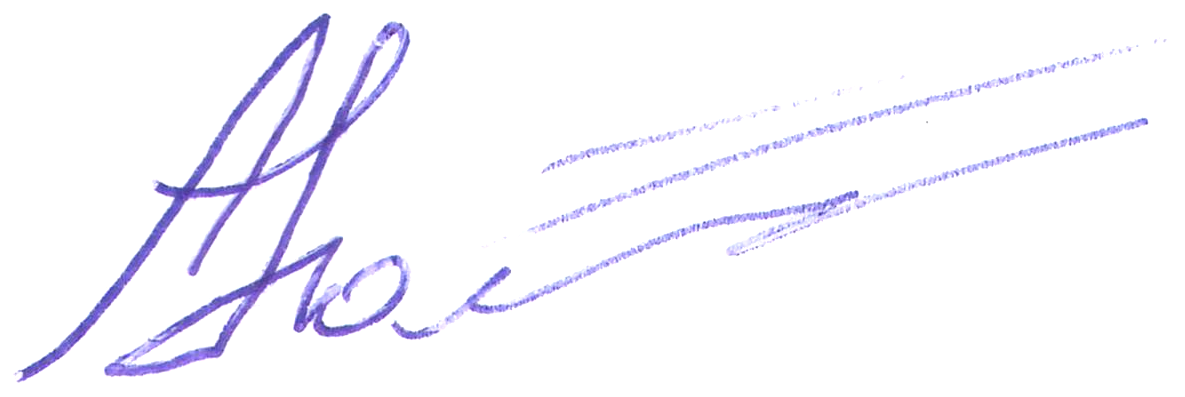
\includegraphics[height=1.7cm]{sign.png}
\end{flushright}
}
%
\vspace{0pt plus6fill} %число перед fill = кратность относительно некоторого расстояния fill, кусками которого заполнены пустые места
\begin{center}
{\large \thesisAuthor}
\end{center}
%
\vspace{0pt plus1fill} %число перед fill = кратность относительно некоторого расстояния fill, кусками которого заполнены пустые места
\begin{center}
\textbf {\large %\MakeUppercase
\thesisTitle}

\vspace{0pt plus2fill} %число перед fill = кратность относительно некоторого расстояния fill, кусками которого заполнены пустые места
{%\small
Специальность \thesisSpecialtyNumber\ "---

<<\thesisSpecialtyTitle>>
}

\ifdefined\thesisSpecialtyTwoNumber
{%\small
Специальность \thesisSpecialtyTwoNumber\ "---

<<\thesisSpecialtyTwoTitle>>
}
\fi

\vspace{0pt plus2fill} %число перед fill = кратность относительно некоторого расстояния fill, кусками которого заполнены пустые места
Диссертация на соискание учёной степени

\thesisDegree
\end{center}
%
\vspace{0pt plus4fill} %число перед fill = кратность относительно некоторого расстояния fill, кусками которого заполнены пустые места
\begin{flushright}
\ifdefined\supervisorTwoFio
Научные руководители:

\supervisorRegalia

\ifdefined\supervisorDead
\framebox{\supervisorFio}
\else
\supervisorFio
\fi

\supervisorTwoRegalia

\ifdefined\supervisorTwoDead
\framebox{\supervisorTwoFio}
\else
\supervisorFio
\fi
\else
Научный руководитель:

\supervisorRegalia

\ifdefined\supervisorDead
\framebox{\supervisorFio}
\else
\supervisorFio
\fi
\fi

\end{flushright}
%
\vspace{0pt plus4fill} %число перед fill = кратность относительно некоторого расстояния fill, кусками которого заполнены пустые места
{\centering\thesisCity\ "--- \thesisYear\par}
           % Титульный лист
% Оглавление (ГОСТ Р 7.0.11-2011, 5.2)
\ \\ \ \\
\ifdefmacro{\microtypesetup}{\microtypesetup{protrusion=false}}{} % не рекомендуется применять пакет микротипографики к автоматически генерируемому оглавлению
\tableofcontents*
\addtocontents{toc}{\protect\tocheader}
\endTOCtrue
\ifdefmacro{\microtypesetup}{\microtypesetup{protrusion=true}}{}        % Оглавление
\ifnumequal{\value{contnumfig}}{1}{}{\counterwithout{figure}{chapter}}
\ifnumequal{\value{contnumtab}}{1}{}{\counterwithout{table}{chapter}}
\chapter*{Введение}                         % Заголовок
\addcontentsline{toc}{chapter}{Введение}    % Добавляем его в оглавление

\newcommand{\actuality}{\textbf{\actualityTXT}}
\newcommand{\progress}{\textbf{\progressTXT}}
\newcommand{\aim}{\textbf{\aimTXT}}
\newcommand{\tasks}{\textbf{\tasksTXT}}
\newcommand{\novelty}{\textbf{\noveltyTXT}}
\newcommand{\influence}{\textbf{\influenceTXT}}
\newcommand{\methods}{\textbf{\methodsTXT}}
\newcommand{\defpositions}{\textbf{\defpositionsTXT}}
\newcommand{\reliability}{\textbf{\reliabilityTXT}}
\newcommand{\probation}{\textbf{\probationTXT}}
\newcommand{\contribution}{\textbf{\contributionTXT}}
\newcommand{\publications}{\textbf{\publicationsTXT}}

\textbf{Актуальность темы.}
На сегодняшний день взаимодействие человека с компьютерными системами через управление речевыми командами является одним из самых удобных и перспективных форматов.

% версия для автореферата
%Первая попытка конструирования системы автоматического распознавания речи была сделана в 1952 году, а уже в 1970-е годы исследования в области распознавания речи достигли значительных успехов.
%До настоящего времени распознавание речи совершенствовалось, а словарь распознаваемых слов вырос до нескольких десятков тысяч.
%Применение быстрых методов декодирования позволило производить распознавание в реальном времени.

% версия для диссертации
Первая попытка конструирования системы автоматического распознавания речи была сделана в 1952 году в Bell Laboratories, США~\cite{davis1952automatic}.
Система с хорошим уровнем точности распознавала цифры от нуля до девяти, произнесённые диктором через телефонный автомат.
Значительные улучшения качества в области распознавания речи были достигнуты в 70-ых годах.
В то время технологии автоматического распознавания отдельных команд основывалась на работах Itakura в США~\cite{itakura1975minimum}, Sakoe и Chiba в Японии~\cite{sakoe1978dynamic} и Величкина и Загоруйка в СССР~\cite{velichko1970automatic}.
Советские учёные производили улучшения методов распознавания с помощью эталона.
Применение подхода динамического программирования было отличительной особенностью японского исследования.
Работа Itakura раскрыла метод кодирования линейного предсказания (Linear Predictive Coding, LPC), который успешно использовался в распознавании сигналов с низким битрейтом (количество битов информации, передаваемых в секунду).
В AT\&T Bell Laboratories были построены распознающие системы, обработка акустического сигнала в которых была основана на LPC анализе, а процесс распознавания проходил с использованием метода динамической трансформации времени (Dynamic Time Warping, DTW).
В 1980-х годах от подходов, основанных на применении эталонов, научные работы в области распознавания речи перешли к моделированию статистическими методами.
Использовались скрытые модели Маркова (Hidden Markov Models, HMM).
Работы Бейкера~\cite{baker1990stochastic} были одними из первых, в которых для решения задачи распознавания речи были применены HMM.
С 1990-х годов распознавание речи несколько усовершенствовалось.
Словарь распознаваемых слов вырос до нескольких десятков тысяч.
Использование быстрых методов декодирования позволило производить распознавание в реальном времени.
В современных дикторозависимых системах, распознающих отдельные слова, количество которых достигает двадцати тысяч слов, ошибки составляют менее 0.1~\%~\cite{das1993influence}.
И около 5~\% ошибок в независимых от диктора системах, которые распознают слитную речь из тысячи слов~\cite{aubert1993continuous}.

В современных системах применяются 3 основные группы методов распознавания речи.
Первая группа --- это скрытые марковские модели.
В них входная речь рассматривается как последовательность фонем с определёнными вероятностями перехода.
Распознавание производится через поиск наиболее вероятной последовательности фонем для данного входного сигнала.
Вторая --- это методы, основанные на сравнении с эталоном.
Для каждого слова из словаря некоторым образом составляется эталон.
При распознавании выбирается то слово, эталон которого наиболее близок к входному сигналу.
Третья группа методов основана на искусственных нейронных сетях.
Суть методов состоит в нахождении такой решающей функции, которая по входному сигналу может определить его принадлежность к определённому классу.
Искусственные нейронные сети построены по принципу организации биологических нейронных сетей и хорошо справляются с широким спектром задач.

В данной работе решается задача повышения вероятности правильных распознаваний и снижения влияния акустических шумов путём разработки и совершенствования алгоритмов распознавания команд речевого интерфейса пилота для управления бортовым оборудованием современных самолётов.
По сравнению с обычной задачей распознания речи к речевому интерфейсу кабины пилота предъявляются следующие требования:

\begin{itemize}
	\item распознавание ограниченного словаря из слов или фраз;
	\item компактность, автономность, высокое быстродействие;
	\item хорошее качество распознавания в условиях сильного шума.
\end{itemize}

% версия для автореферата
%С учётом этих требований широко используемые скрытые марковские модели не подходят из-за низкого качества распознавания в условиях шума.
% версия для диссертации
С учётом этих требований широко используемые скрытые марковские модели не подходят из-за низкого качества распознавания в условиях шума \cite{korsun2013experimental}.

Остальные две группы методов в настоящий момент не обеспечивают необходимой надёжности распознавания.
По этой причине тема настоящей работы, направленной на совершенствование методов распознавания речевых команд с помощью сравнения с эталоном и с использованием нейронных сетей, является актуальной.
Исследования, выполненные в рамках данной работы, направлены на решение таких практически значимых и актуальных задач, как предобработка входящего сигнала путём выделения однородных частей, улучшение качества эталонов с помощью выделения в них главных компонент и использование систем распознавания из нескольких эталонов.
В работе также проведено обширное экспериментальное исследование всех разработанных методов на различных наборах входных данных с несколькими уровнями шума.

\textbf{Объект и предмет исследования.}
В работе в качестве объекта исследования рассматриваются речевые команды, а предметами исследования являются методы и алгоритмы распознавания речевых команд.

\textbf{Целью} работы является повышение вероятности правильных распознаваний и снижение влияния акустических шумов, путём разработки алгоритмического обеспечения для распознавания команд речевого интерфейса кабины пилота в виде отдельных слов и фраз.
За рамками работы остались выбор оптимального состава команд и их интерпретация.

Для достижения поставленной цели решаются следующие научно-технические задачи:
\begin{itemize}
	\item анализ статистических свойств речевых команд и их нормализация;
	\item разработка алгоритмов предварительного разбиения записей на однородные части;
	\item разработка алгоритмов исключения шума и выделения наиболее значимых компонент в эталоне;
	\item исследование статистических закономерностей верного и неверного распознавания речевых команд и их использование для уменьшения количества ошибок;
	\item разработка алгоритмов использования нескольких эталонов одного слова для улучшения качества распознавания;
	\item исследование современных типов и архитектур искусственных нейронных сетей глубокого обучения для применения в задаче распознавания речевых команд.
\end{itemize}

\textbf{Методология и методы исследования.}
Основными методами исследования, используемыми в работе, являются: анализ данных, цифровая обработка сигналов, теория вероятностей, математическая статистика, численная оптимизация, проектирование программных средств.

\textbf{Научная новизна} заключается в разработке совокупности алгоритмов, обеспечивающих повышение вероятности правильных распознаваний команд речевого интерфейса кабины пилота:
\begin{itemize}
	\item алгоритм разбиения речевых команд на фонетически однородные части на основе модифицированного метода динамического программирования;
	\item алгоритм оптимизации эталонов на основе метода главных компонент;
	\item алгоритм оптимизации размерности параметрических портретов с использованием полиномов Чебышёва;
	\item алгоритм распознавания команд по нескольким эталонам с использование байесовского подхода и метода комитетов;
	\item алгоритм распознавания команд нейронными сетями глубокого обучения, способных обучаться на выборках малого размера.
\end{itemize}

\textbf{Практическая значимость.}
Полученная в результате работы совокупность алгоритмов обеспечивает высокую точность распознавания речевых команд при различных уровнях шума, в том числе с учётом случая статически неустойчивого самолёта.
Результаты работы могут быть применены в учебном процессе и в ходе разработки алгоритмического обеспечения речевого интерфейса пилота для таких задач, как отображение информации, выбор частоты радиооборудования, прокладка маршрута, управление системой опознавания и датчиками, запрос запаса топлива.

\textbf{Положения, выносимые на защиту:}
\begin{enumerate}[label={\arabic*)}]
	\item Разработан алгоритм разбиения речевых команд на фонетически однородные части, отличающийся от существующих применением модифицированного метода динамического программирования.
	\item Разработан алгоритм оптимизации эталонов, отличающийся от существующих тем, что искомый эталон формируется как линейная комбинация главных компонент, оптимизирующая заданный критерий качества.
	\item Разработан алгоритм оптимизации размерности параметрических портретов, отличающийся выделением наиболее значимых составляющих с использованием полиномов Чебышёва.
	\item Разработан алгоритм распознавания команд по нескольким эталонам, отличающийся применением последовательного оценивания с расчётом апостериорных байесовских вероятностей.
	\item Разработан алгоритм распознавания команд нейронными сетями глубокого обучения, отличающийся от существующих обучением на выборке малого размера.
\end{enumerate}

\textbf{Достоверность результатов} обеспечивается корректным применением математической статистики, методов идентификации и анализа данных, подтверждением полученных теоретических результатов с помощью экспериментов, а также сравнением с известными результатами, ранее полученными другими авторами.

% версия для автореферата
%\textbf{Апробация работы.}
%Основные результаты исследования докладывались на следующих конференциях:
%\begin{enumerate}[label={\arabic*)}]
%	\item Доклад <<Получение оптимального эталона с помощью метода главных компонент>> на Всероссийской научно-технической конференции <<XII Научные чтения по авиации, посвящённые памяти Н.Е. Жуковского>> (Москва, 2015) \cite{poliyev2015pca}.
%	\item Доклад <<Алгоритм разбиения слов на однородные части в интересах разработки речевого интерфейса бортового оборудования>> на Восьмом Международном Аэрокосмическом Конгрессе IAC'15 (Москва, 2015) \cite{poliyev2015split}.
%	\item Доклад <<Разработка модифицированного алгоритма динамического программирования для разбиения слов на однородные части>> на Всероссийской научно-технической конференции <<XIII Научные чтения по авиации, посвящённые памяти Н.Е. Жуковского>> (Москва, 2016) \cite{poliyev2016dynamic}.
%	\item Доклад <<Определение оптимального разбиения слова на однородные участки на основе матрицы корреляционного портрета>> на Юбилейной Всероссийской научно-технической конференции <<Авиационные системы в XXI веке>> (Москва, 2016) \cite{poliyev2016split, poliyev2017split}.
%	\item Доклад <<Разработка метода анализа фонетически однородных частей слов естественного языка>> на Второй Международной научно-практической конференции <<Эрго-2016: Человеческий фактор в сложных технических системах и средах>> (Санкт-Петербург, 2016) \cite{poliyev2016natural}.
%	\item Доклад <<The algorithm of an optimal word pattern synthesis using principal component analysis>> на международном семинаре Workshop on Contemporary Materials and Technologies in the Aviation Industry --- CMTAI (Москва, 2016) \cite{poliyev2016pca}.
%	\item Доклад <<Применение формулы Байеса для распознавания слов с использованием нескольких эталонов>> на Всероссийской научно-технической конференции <<Навигация, наведение и управление летательными аппаратами>> (Москва, 2017) \cite{poliyev2017bayes}.
%	\item Доклад <<Разработка алгоритма распознавания слов в условиях шума на основе свёрточных нейронных сетей>> на Девятом Международном Аэрокосмическом Конгрессе IAC'18 (Москва, 2018) \cite{poliyev2018cnn}.
%	\item Доклад <<Распознавание речевых команд на основе свёрточных нейронных сетей>> на Всероссийской научно-технической конференции <<Моделирование авиационных систем>> (Москва, 2018) \cite{poliyev2018cnn2}.
%\end{enumerate}
%
%\textbf{Публикации.}
%По теме диссертации автором опубликовано 4 научных работы \cite{korsun2016automatic,poliyev2017pca,korsun2018usage,korsun2018optimal}: 3 из них в изданиях из списка, рекомендованного ВАК РФ \cite{korsun2016automatic,poliyev2017pca,korsun2018usage}, и 2 из них в изданиях, входящих в базу Scopus и базу Web of Science \cite{korsun2016automatic,korsun2018optimal}.

% версия для диссертации
\textbf{Апробация работы.}
Основные результаты исследования докладывались на следующих конференциях:
\begin{enumerate}[label={\arabic*)}]
	\item Доклад на Всероссийской научно-технической конференции <<XII Научные чтения по авиации посвящённые памяти Н.Е. Жуковского>> (Москва, 17 апреля 2015 года).
	Тема доклада: <<Получение оптимального эталона с помощью метода главных компонент>>.
	Текст доклада напечатан в сборнике докладов конференции \cite{poliyev2015pca}.
	\item Доклад на Восьмом Международном Аэрокосмическом Конгрессе IAC'15 (Москва, 28--31 августа 2015 года).
	Тема доклада: <<Алгоритм разбиения слов на однородные части в интересах разработки речевого интерфейса бортового оборудования>>.
	Текст доклада напечатан в сборнике докладов конференции \cite{poliyev2015split}.
	\item Доклад на Всероссийской научно-технической конференции <<XIII Научные чтения по авиации посвящённые памяти Н.Е. Жуковского>> (Москва, 14 апреля 2016 года).
	Тема доклада: <<Разработка модифицированного алгоритма динамического программирования для разбиения слов на однородные части>>.
	Текст доклада напечатан в сборнике докладов конференции \cite{poliyev2016dynamic}.
	\item Доклад на Юбилейной Всероссийской научно-технической конференции <<Авиационные системы в XXI веке>> (Москва, 26 мая 2016 года).
	Тема доклада: <<Определение оптимального разбиения слова на однородные участки на основе матрицы корреляционного портрета>>.
	Текст доклада напечатан в сборнике докладов конференции \cite{poliyev2016split, poliyev2017split}.
	\item Доклад на Второй Международной научно-практической конференции <<Эрго-2016: Человеческий фактор в сложных технических системах и средах>> (Санкт-Петербург, 6--9 июля 2016 года).
	Тема доклада: <<Разработка метода анализа фонетически однородных частей слов естественного языка>>.
	Текст доклада напечатан в сборнике докладов конференции \cite{poliyev2016natural}.
	\item Доклад на международном семинаре Workshop on Contemporary Materials and Technologies in the Aviation Industry --- CMTAI (Москва, 15--16 декабря 2016 года).
	Тема доклада: <<The algorithm of an optimal word pattern synthesis using principal component analysis>>.
	Текст доклада напечатан в сборнике докладов конференции \cite{poliyev2016pca}.
	\item Доклад на Всероссийской научно-технической конференции <<Навигация, наведение и управление летательными аппаратами>> (Москва, 21--22 сентября 2017 года).
	Тема доклада: <<Применение формулы Байеса для распознавания слов с использованием нескольких эталонов>>.
	Текст доклада напечатан в сборнике докладов конференции \cite{poliyev2017bayes}.
	\item Доклад на Девятом Международном Аэрокосмическом Конгрессе IAC'18 (Москва, 28--31 августа 2018 года).
	Тема доклада: <<Разработка алгоритма распознавания слов в условиях шума на основе свёрточных нейронных сетей>>.
	Текст доклада напечатан в сборнике докладов конференции \cite{poliyev2018cnn}.
	\item Доклад на Всероссийской научно-технической конференции <<Моделирование авиационных систем>> (Москва, 21--22 ноября 2018 года).
	Тема доклада: <<Распознавание речевых команд на основе свёрточных нейронных сетей>>.
	Текст доклада напечатан в сборнике докладов конференции \cite{poliyev2018cnn2}.
\end{enumerate}

\textbf{Публикации.}
По теме диссертации автором опубликовано 4 научных работы \cite{korsun2016automatic,poliyev2017pca,korsun2018usage,korsun2018optimal}: 3 из них в изданиях из списка, рекомендованного ВАК РФ \cite{korsun2016automatic,poliyev2017pca,korsun2018usage}, и 2 из них в изданиях, входящих в базу Scopus и базу Web of Science \cite{korsun2016automatic,korsun2018optimal}.
\begin{enumerate}[label={\arabic*)}]
	\item Статья <<Автоматическое выделение фонетически однородных участков в словах естественного языка на основе многопараметрической оптимизации>> в журнале <<Известия Российской академии наук. Теория и системы управления>>, 2016 год, № 4, страницы 145–-154 \cite{korsun2016automatic}.
	\item Статья <<Разработка алгоритма синтеза оптимальных эталонов на основе метода главных компонент>> в журнале <<Cloud of science>>, 2017 год, № 4, страницы 650--661 \cite{poliyev2017pca}.
	\item Статья <<Использование нескольких эталонов при распознавании речи: формула Байеса и метод комитетов>> в журнале <<Вестник компьютерных и информационных технологий>>, 2018 год, № 1, страницы 14--23 \cite{korsun2018usage}.
	\item Статья <<Optimal pattern synthesis for speech recognition based on principal component analysis>> в журнале <<IOP Conference Series: Materials Science and Engineering>>, 2018 год, № 312, страницы 12--14 \cite{korsun2018optimal}.
\end{enumerate}

 % Характеристика работы по структуре во введении и в автореферате не отличается (ГОСТ Р 7.0.11, пункты 5.3.1 и 9.2.1), потому её загружаем из одного и того же внешнего файла, предварительно задав форму выделения некоторым параметрам

\textbf{Объем и структура работы.} Диссертация состоит из введения, четырёх разделов и заключения.
%% на случай ошибок оставляю исходный кусок на месте, закомментированным
%Полный объём диссертации составляет  \ref*{TotPages}~страницу с~\totalfigures{}~рисунками и~\totaltables{}~таблицами. Список литературы содержит \total{citenum}~наименований.
%
Полный объём диссертации составляет
\formbytotal{TotPages}{страниц}{у}{ы}{}, включая
\formbytotal{totalcount@figure}{рисун}{ок}{ка}{ков} и
\formbytotal{totalcount@table}{таблиц}{у}{ы}{}.   Список литературы содержит
\formbytotal{citenum}{наименован}{ие}{ия}{ий}.
    % Введение
\ifnumequal{\value{contnumfig}}{1}{\counterwithout{figure}{chapter}
}{\counterwithin{figure}{chapter}}
\ifnumequal{\value{contnumtab}}{1}{\counterwithout{table}{chapter}
}{\counterwithin{table}{chapter}}
\chapter{Обзор подходов к формированию речевого интерфейса бортового оборудования современных самолётов} \label{chapt1}

\section{Анализ области применения речевых интерфейсов} \label{sect1_1}

Рациональная и надёжная организация человеко-машинного взаимодействия является одной из важных задач современной техники \cite{evdokimenkov2015use, polyak2017principle, kolokolov2006obrabotka, sebryakov2007problems}.
С развитием речевых технологий, главным образом, систем автоматического распознавания речи, связывают будущее голосовых интерфейсов интеллектуальных систем управления различными техническими системами и подвижными объектами.
Для повышения уровня безопасности полёта необходимо нивелировать нагрузку от задач, отвлекающих пилота от выполнения его основных функций.
Поэтому в последнее время активно разрабатывается речевой интерфейс управления бортовым оборудованием летательных аппаратов \cite{bandaros2007sistema, bandaros2009issledovanie, korsun2011synthesis, evdokimenkov2015use}.

За рубежом речевые командные системы голосового управления уже внедряются в бортовые информационные системы летательных аппаратов.
Ведутся интенсивные разработки речевого интерфейса фирмой Eurofighter GmbH в Евросоюзе для самолёта Eurofighter Typhoon, фирмой Lockheed Martin Corporation в США для истребителей F-16 и F-35, а также другими фирмами.

На истребителе Eurofighter Typhoon с 2005 года эксплуатируется дикторозависимая система Direct Voice Input (DVI) \cite{eurofighter2005}, основанная на сравнении с эталонами.
Система имеет словарь размером более 100 команд --- тех, которые не связаны непосредственно с процессом полёта или использованием вооружения.
Direct Voice Input используется для управления вспомогательным бортовым оборудованием: режимами работы радара, индикацией на приборной панели и графических экранах, навигационными средствами, заданием частот настройки радиоаппаратуры, системой радиолокационного опознавания <<свой-чужой>> и так далее \cite{eurofighter2016}.

Также в рамках программы Advanced Fighter Technology Integration для истребителей F-16A и F-35 была разработана система Voice-Controlled Interactive Device, созданная компанией Lear Siegler \cite{f16vcid}.
Данная система имеет словарь до 256 слов, позволяет распознавать команды в виде фраз и показывает вероятность распознавания более 90~\%.
Основное препятствие для улучшения качества распознавания состоит в уровне шума в кабине пилота, который может достигать 120 дБ во время маневров.
Кроме этого, не так много пилотов сохраняют способность говорить при перегрузках больших, чем 5 g.

Аналогичные системы голосового управления используются на французских истребителях Dassault Rafale \cite{dassault} и франко-британском вертолёте Aérospatiale Gazelle \cite{gazelle}.

Для сравнения можно привести результаты распознавания речи, достигаемые в других областях.
Компания Google использует технологии распознавания речи для голосового ввода команд на компьютерах и мобильных устройствах.
В последние годы наблюдается последовательное снижение ошибок распознавания свободной речи с 23~\% в 2013 году и 8~\% в 2015 году до 4.9~\% в 2017 году \cite{google2017speech}.
Заметное снижение процента ошибок распознавания связано, в основном, с началом использования глубоких нейронных сетей \cite{chan2018speech}.
Также следует отметить, что при распознавании речи в условиях шума процент ошибок увеличивается лишь незначительно \cite{chan2016listen}.

В качестве сравнения, важно оценить вероятность распознавания речи человеком.
В этой задаче процент ошибок распознавания сильно зависит от характеристик словаря и условий распознавания \cite{lippmann1997speech}.
Самая маленькая ошибка величиной 0.1~\% достигается при распознавании записей цифр, тогда как записи букв из алфавита распознаются с 1.6~\% ошибок.
Также получается 1~\% ошибок при распознавании записей предложений из делового журнала, 2~\% при распознавании записей предложений не несущих смысла и 4~\% ошибок при распознавании телефонных разговоров.

Как видно из приведённых результатов распознавания различных вариантов речи, свободная речь распознаётся заметно хуже изолированных слов.
Кроме этого, короткие команды обычно имеют чёткую интерпретацию, тогда как свободную речь заметно сложнее преобразовать в команды панели управления самолётом.
Также распознавание отдельных слов, очевидно, требует меньше вычислительной мощности, что важно в условиях её ограниченности и автономности.
Так как высокая вероятность правильного распознавания команд является одним из главных требований речевого интерфейса кабины пилота, имеет смысл распознавать команды в виде слов и иногда в виде коротких фраз.

Другим важнейшим требованием, предъявляемым к интерфейсу управления бортовым оборудованием самолёта, является высокая вероятность правильного распознавания слов в условиях сильных шумов и помех, что стимулирует создание помехоустойчивых алгоритмов \cite{bandaros2008usage, korsun2014algo, korsun2012results, korsun2013experimental, hirsch2000aurora, schmidt2000speech}.
Требования по помехозащищённости подробно описаны в руководствах \cite{aviaizdat2010p4754, aviaizdat2010p4761}.
Существенную роль играют временные затраты используемого алгоритма, которые следует учитывать при разработке комплекса программ для бортового оборудования.

Сложность бортового оборудования постоянно возрастает, поэтому необходимы дополнительные независимые каналы связи пилота и бортовой системы.
В перечень решаемых задач могут входить: управление индикацией в кабине пилота, изменение рабочей частоты связи и радионавигационного оборудования, изменение частоты передачи сигналов приёмоответчика, управление бортовой радиолокационной станцией и многие другие действия.
Необходимо отметить, что целесообразным является управление с помощью речевого интерфейса теми системами, которые не снижают уровень безопасности полёта.
Таким образом, необходимым условием при реализации речевого интерфейса является полное соответствие требованиям по безопасности полёта.

Речевые технологии могут использоваться не только для автоматической интерпретации естественного языка \cite{benesty2007springer, rabiner1979cifrovaya}, но и для тестирования уровня усталости оператора \cite{korsun2012method, bandaros2010opredelenie} или его слуховых качеств \cite{ivanov2014investigation, ivanov2017experimental}.

%Целевые значения для бортового оборудования по точности распознавания команд, не влияющих на безопасность полётов, не должны превышать $p=10^{-3}$ отказов в час \cite{aviaizdat2010p4761}.
%Другими словами, на каждую тысячу произнесённых команд в час можно допустить не более одного неправильного распознавания команды.
%Для рассматриваемой задачи получается, что процент правильных распознаваний не должен быть ниже чем 99.9~\%.
%В реальности, при создании дикторонезависимой системы распознавания команд более реалистичными будут значения порядка 98--99~\% при условии сильного шума и различных особенностей речи пилотов.
%На практике для достижение требуемой точности в 99.9~\% может быть использована функция подтверждения или отклонения произнесённой команды с помощью дополнительной клавиши.
%Это позволит отменить произнесённую команду в случае её неверного распознавания.

Ещё не созданы нормативы, задающие процент ошибок для подобных речевых систем, поэтому в данной работе ставилась цель получить процент ошибок сопоставимый с процентом ошибок при распознавании речи человеком.
На практике для повышения точности распознавания может быть использована функция подтверждения или отклонения произнесённой команды с помощью дополнительной клавиши.
Это позволит отменить произнесённую команду в случае её неверного распознавания.

Также, ошибки распознавания могут привести к последствиям разного типа, но в данной работе принимается гипотеза о том, что ошибки первого и второго рода нежелательны в одинаковой степени.
Поэтому применяется критерий максимума апостериорной вероятности Зигерта-Котельникова, который даёт максимальную вероятность правильных распознаваний.

%\newpage
%============================================================================================================================

\section{Способы параметризации голосовых сигналов} \label{sect1_2}

Входные данные обычно представляют собой звуковой сигнал, как правило хранящийся в формате MP3 (Moving Picture Experts Group-1/2/2.5 Layer 3) или WAV (Waveform Audio File Format).
Формат MP3 использует алгоритм сжатия звукового сигнала с потерями, некритичными для восприятия на слух на непрофессиональной аппаратуре, но существенными при использовании более качественной звуковой системы \cite{mp3}.
При этом главным преимуществом данного формата является заметное снижение размера файла со звуковой записью.

В свою очередь, формат WAV используется для хранения несжатого звука, при этом также является стандартом для оцифрованного аудиопотока и совместим со всеми операционными системами \cite{wav}.

Отсутствие сжатия и сохранение максимально возможного качества записи является критичным условием для задачи распознавания речи, поэтому в работе будут использоваться записи звуковых сигналов только в формате WAV.
Также для дальнейшей работы со звуковыми файлами их нужно преобразовать в более удобное для обработки представление.

%\newpage
%============================================================================================================================

\subsection{Алгоритм частотно-временного квантования} \label{sect1_2_1}

Вариант преобразования входного речевого сигнала, используемый в данной работе, заключается в получении параметрического портрета и состоит в следующем.
В первую очередь сам сигнал речи разделяется на одинаковые по размеру временные интервалы по 10--30 мс, а уже после каждый из них разделяется на 30--40 частотных полос \cite{evdokimenkov2015use, kolokolov2015compare}.
Затем применяется ряд стандартных процедур цифровой переработки данных: увеличение значений высокочастотных компонент, применение окна Ханна для взвешивания интервалов, быстрое преобразование Фурье, частотное осреднение и логарифмирование спектральных плотностей \cite{kolokolov2006obrabotka, oppenheim1999discrete}.
Далее будет подробно рассмотрен каждый из этих этапов.

Речевой сигнал для обработки в системе автоматического распознавания должен быть преобразован в некоторый набор параметров, обычно представляемый матрицей.
В работе рассматривается следующая последовательность преобразований исходного временного сигнала.

Сначала необходимо скорректировать сигнал для увеличения вклада высокочастотных составляющих:
\begin{equation}
x(n) = u(n) - \alpha u(n-1), \qquad \alpha = 0.85 \dots 0.98,
\end{equation}
\begin{itemize}[align=left,leftmargin=1.8em,itemindent=0pt,labelsep=0pt,labelwidth=1.8em]
	\item[где] $u$ --- значение сигнала перед предварительной коррекцией,
	\item[] $n$ --- номер измерения значения сигнала.
\end{itemize}

Затем сигнал разбивается на отдельные частично перекрывающиеся интервалы:
\begin{equation}
s_m(n) = x(m \Delta n + n),\quad
0 \le n \le N_{FFT} - 1,\quad
\Delta n = N_{FFT} - \epsilon N_{FFT},
\end{equation}
\begin{itemize}[align=left,leftmargin=1.8em,itemindent=0pt,labelsep=0pt,labelwidth=1.8em]
	\item[где] $N_{FFT}$ --- длина интервала для быстрого преобразования Фурье,
	\item[] $\epsilon$ --- величина отношения длительности участка перекрытия к длительности интервала, $0 \le \epsilon \le 0.5$,
	\item[] $m$ --- порядковый номер интервала.
\end{itemize}

Для снижения эффекта <<растекания>> спектра, необходимо взвешивать все интервалы окном Хэмминга или Ханна \cite{harris1978usage}.

Окно Хэмминга:
\begin{equation}
w_{H1} = 0.54 - 0.46 \cos \left(\frac{2 \pi n}{N_{FFT} - 1} \right).
\end{equation}

Окно Ханна:
\begin{equation}
w_{H2} = 0.5 \left(1 - \cos \left(\frac{2 \pi n}{N_{FFT} - 1} \right) \right).
\end{equation}

Итоговое значение интервала рассчитывается следующим образом:
\begin{equation}
s_m^{w}(n) = w_{H2}(n) s_m(n).
\end{equation}

Далее вычисляется быстрое преобразование Фурье и его модуль:
\begin{equation}
X_m(k) = FFT\{ s_m(n)^w \} = \sum_{n=0}^{N_{FFT} - 1} s_m^{w}(n) \exp{\left(j\frac{2 \pi k n}{N_{FFT}} \right)},
\end{equation}
\begin{equation}
A_m(k) = |X_m(k)| = \sqrt{Re^2(X_m(k)) + Im^2(X_m(k))}.
\end{equation}

В конце рассчитывается логарифм усреднённого модуля, что соответствует логарифмированию оценок спектральных плотностей:
\begin{equation}
S_m(f_i) = \log\left(\frac{1}{\Delta k} \sum_{k=k_{i,min}}^{k_{i,max}} A_m(k)\right),
\end{equation}
\begin{itemize}[align=left,leftmargin=1.8em,itemindent=0pt,labelsep=0pt,labelwidth=1.8em]
	\item[где] $k_{i,\min}$, $k_{i,\max}$ --- индексы первой и последней частот в спектральной полосе,
	\item[] $\Delta k = k_{i,\max} - k_{i,\min} + 1$,
	\item[] $A_m(k)$ --- модуль преобразования Фурье (или ширина спектральной полосы, не зависит от номера полосы).
\end{itemize}

\begin{equation}
k_{i,min} = \left\lfloor\frac{N_{FFT}}{f_s} \left(f_{min} + \frac{f_{max} - f_{min}}{N_{frb}} (i-1) \right)\right\rfloor + 1, \qquad i = 2 \dots N_{frb},
\end{equation}
\begin{equation}
k_{1,min} = \left\lceil\frac{N_{FFT}}{f_s} f_{min} \right\rceil,
\end{equation}
\begin{equation}
k_{i,max} = \left\lfloor\frac{N_{FFT}}{f_s} \left(f_{min} + \frac{f_{max} - f_{min}}{N_{frb}} i \right)\right\rfloor, \qquad i = 1 \dots N_{frb},
\end{equation}
\begin{equation}
f_i = f_{min} + \frac{f_{max} - f_{min}}{N_{frb}} \left(i + \frac{1}{2} \right), \qquad i = 1 \dots N_{frb},
\end{equation}
\begin{itemize}[align=left,leftmargin=1.8em,itemindent=0pt,labelsep=0pt,labelwidth=1.8em]
	\item[где] $f_i$ --- частота, соответствующая середине $i$-й полосы,
	\item[] $f_s$ --- частота дискретизации.
\end{itemize}

В итоге, последовательность логарифмов спектра функции в дискретных значениях частоты, рассчитанная на скользящем временном промежутке в 10--30 мс, была выбрана для характеристики речевого сигнала.
Параметрическим портретом слова называются описанные параметры, собранные в одну матрицу.
Спектральная характеристика речевого сигнала на всех временных интервалах отображается в столбцах этого параметрического портрета.

%\newpage
%============================================================================================================================

\subsection{Алгоритм получения эталонов} \label{sect1_2_2}

Эталонный параметрический портрет $E$ можно составить из параметрических портретов $X$ имеющихся записей речевых команд.
Наиболее простым методом вычисления эталона является усреднение значений параметрических портретов небольшого набора реализаций одного и того же слова.
Оптимальным является выбор наиболее <<типичных>> реализаций слова, например, они должны иметь длительность максимально близкую к среднему значению.
После этого можно сравнивать параметрический портрет эталона с параметрическим портретом распознаваемого слова.

%\newpage
%============================================================================================================================

\section{Анализ основных подходов к автоматическому распознаванию речи} \label{sect1_3}

Тремя основными методами распознавания речи являются: сравнение с эталоном, скрытые марковские модели и нейронные сети.
Подробное описание данных методов содержится в следующих подразделах.

%\newpage
%============================================================================================================================

\subsection{Сравнение с эталоном} \label{sect1_3_1}

Традиционно применяемый метод автоматического распознавания речевых команд с помощью эталона использует спектрально-временное преобразование записи входного слова, описанное в подразделе \ref{sect1_2_1}.
Преимуществом данного метода является высокое качество распознавания при высоком уровне шумов во входном сигнале.

Обозначим параметрический портрет распознаваемого слова как $X = \{x_1, x_2, \dots, x_{N_x} \}$, где $x_i$ --- спектральный вектор слова в момент времени $i$, а $N_x$ --- общее количество временных интервалов.
Пусть у нас также есть словарь распознаваемых слов размера $V$.
Тогда обозначим параметрический портрет эталона $j$-го слова, $j = \overline{1, V}$, как $E^j = \{e_1^j, e_2^j, \dots, e_{N_e^j}^j \}$, где аналогично определяются $e_i^j$ --- спектральный вектор $j$-го слова в момент времени $i$, а $N_e^j$ --- общее количество временных интервалов в $j$-м слове.

Задача заключается в том, чтобы оценить расстояние между параметрическим портретом слова $X$ и каждым из эталонов $E^j$.
Критерий максимума коэффициента корреляции векторов, значения которых рассчитаны из исходных матриц параметрических портретов представляет собой один из способов оценки расстояния.
Другая мера близости, Z-преобразование Фишера, будет описана в подразделе \ref{sect1_4_1}.
Также применяются такие меры расстояния как евклидово расстояние, расстояние Минковского и расстояние Махаланобиса \cite{mahalanobis1936generalized}.

При выборе эталона необходимо сравнить распознаваемое слово со всем набором эталонов и выбрать тот, у которого получилось наименьшее расстояние с распознаваемой записью.
В качестве результата распознавания рассматриваемого метода признается речевая команда, которая соответствует данному эталону.

%\newpage
%============================================================================================================================

\subsection{Скрытая марковская модель} \label{sect1_3_2}

Рассмотрим систему, которая в каждый момент времени может находиться в одном из состояний $1, 2, \dots, N$.
Пусть $q_t$ --- это состояние системы в момент $t$.
С течением времени состояние системы изменяется согласно переходной матрице вероятностей $\pmb{A}$, также называемой матрицей перехода.
Главное свойство марковских цепей~\cite{nikolenko2012} заключается в том, что следующее состояние не зависит от всей истории прошлых состояний, а зависит только от непосредственно предыдущего состояния.
Математически это выражается следующим образом: $P(q_t = j | q_{t-1} = i, q_{t-2} = k, \dots)= P(q_t = j | q_{t-1} = i)$.
Другое свойство --- это независимость элементов переходной матрицы вероятностей $a_{ij} = P(q_t = j | q_{t-1} = i)$, $1 \le i$, $j \le N$ от времени.
В итоге, матрица перехода выглядит следующим образом: $\pmb{A} = [a_{ij}]_{N \times N}$.
Чтобы окончательно описать систему, нужно задать начальное распределение вероятностей 
\begin{equation}
\pi =
\begin{bmatrix}
\pi_1 = P(q_1 = 1) \\
\pi_2 = P(q_1 = 2) \\
\vdots \\
\pi_N = P(q_1 = N)
\end{bmatrix}
,\qquad
\sum_{i=1}^N \pi_i = 1.
\end{equation}

Полное описание марковской цепи задаётся с помощью параметров модели: $\pmb{A}$ и $\pmb{\pi}$.

Скрытые марковские цепи являются расширением марковских цепей.
Усложнение заключается в том, что каждое состояние уже не является детерминированным, оно становится вероятностным.
Это означает, что каждое состояние генерирует наблюдение $\pmb{o}_t$, согласно некоторой вероятностной функции.
Вероятность получить наблюдение $\pmb{o}_t$ в состоянии $j$ обозначается $b_j (o_t) = P(o_t | q_t = j)$.
Для всех $N$ состояний и можно сформировать матрицу распределения вероятностей $\pmb{B} = {b_j (o_t)}_{j=1}^N$.
Ещё один элемент скрытой марковской модели $M$ --- размер алфавита, из которого формируется наблюдение $V = {v_k}_{k=1}^M$.
Вероятность получить данные $v_k$ в состоянии $j$ определяется как $b_j (o_t) = b_j (k) = P(o_t = v_k | q_t = j)$.
Модель $\lambda=(\pmb{A}, \pmb{B}, \pmb{\pi})$ состоит из матрицы перехода $\pmb{A}$, матрицы наблюдаемых ${\pmb{B}}$ и начального распределения $\pmb{\pi}$.

Для скрытой марковской модели можно сформировать 3 основные задачи:
\begin{itemize}
	\item первая задача: по данной модели $\lambda$ и последовательности наблюдений $\pmb{O} = (o_1, o_2, \dots, o_T)$ найти вероятность появления последовательности наблюдений $P(\pmb{O}|\lambda)$ --- это нужно для того, чтобы оценить, насколько хорошо модель подходит к данным;
	\item вторая задача: по данной последовательности наблюдений $\pmb{O} = (o_1, o_2, \dots, o_T)$ и модели $\lambda$ найти <<оптимальную>> последовательность состояний $\pmb{q} = (q_1, q_2, \dots, q_T)$;
	\item третья задача: оптимизировать параметры модели $\lambda = (\pmb{A}, \pmb{B}, \pmb{\pi})$ так, чтобы максимизировать $P(\pmb{O} | \lambda)$ при данной последовательности наблюдений $\pmb{O}$.
\end{itemize}

Первую задачу можно рассматривать как задачу распознавания.
При некотором заданном множестве моделей, где каждая модель представляет слово, какая модель наиболее вероятна при данном наблюдении, то есть какое слово произнесли?
Суть второй задачи состоит в попытке восстановить скрытую часть модели.
Третья задача --- это задача обучения.
Дана обучающая последовательность, нужно построить модель для каждого слова.
Она является наиболее значимой, т.к. она позволяет оптимальным образом подобрать параметры модели к последовательности наблюдений.

Скрытые марковские модели хорошо подходят для распознавания свободной речи.
Но для их применения необходимо использовать некоторые заранее заданные модели языка.
Другим недостатком являются плохие результаты распознавания в условиях шума.

%\newpage
%============================================================================================================================

\subsection{Искусственные нейронные сети} \label{sect1_3_3}

Искусственная нейронная сеть представляет собой математическую модель и соответствующее программное обеспечение, построенное по принципу организации биологических нейронных сетей.
Последние обычно состоят из головного мозга, спинного мозга и периферической нервной системы.
Нейронная сеть состоит из группы связанных нейронов, при этом общее количество нейронов и связей между ними может быть достаточно большим.
Как правило, искусственный нейрон представляется как нелинейная функция от линейной комбинации входных сигналов.
Структурно он состоит из синапсов, каждому из которых соответствует определённый вес синаптической связи, сумматора и функции активации \cite{haykin2008neuron}.
Введём следующие обозначения: $x_1, \dots, x_N$ --- выходные сигналы, приходящие от других нейронов; $w_1, \dots, w_N$ --- синаптические веса нейрона; $b$ --- пороговое значение (порог); $\phi(\nu)$ --- функция активации; $y$ --- выходной сигнал нейрона.
На рисунке \ref{fig:artificalNeuron} схематически представлена модель искусственного нейрона. 

\begin{figure}[h]
	\centering
	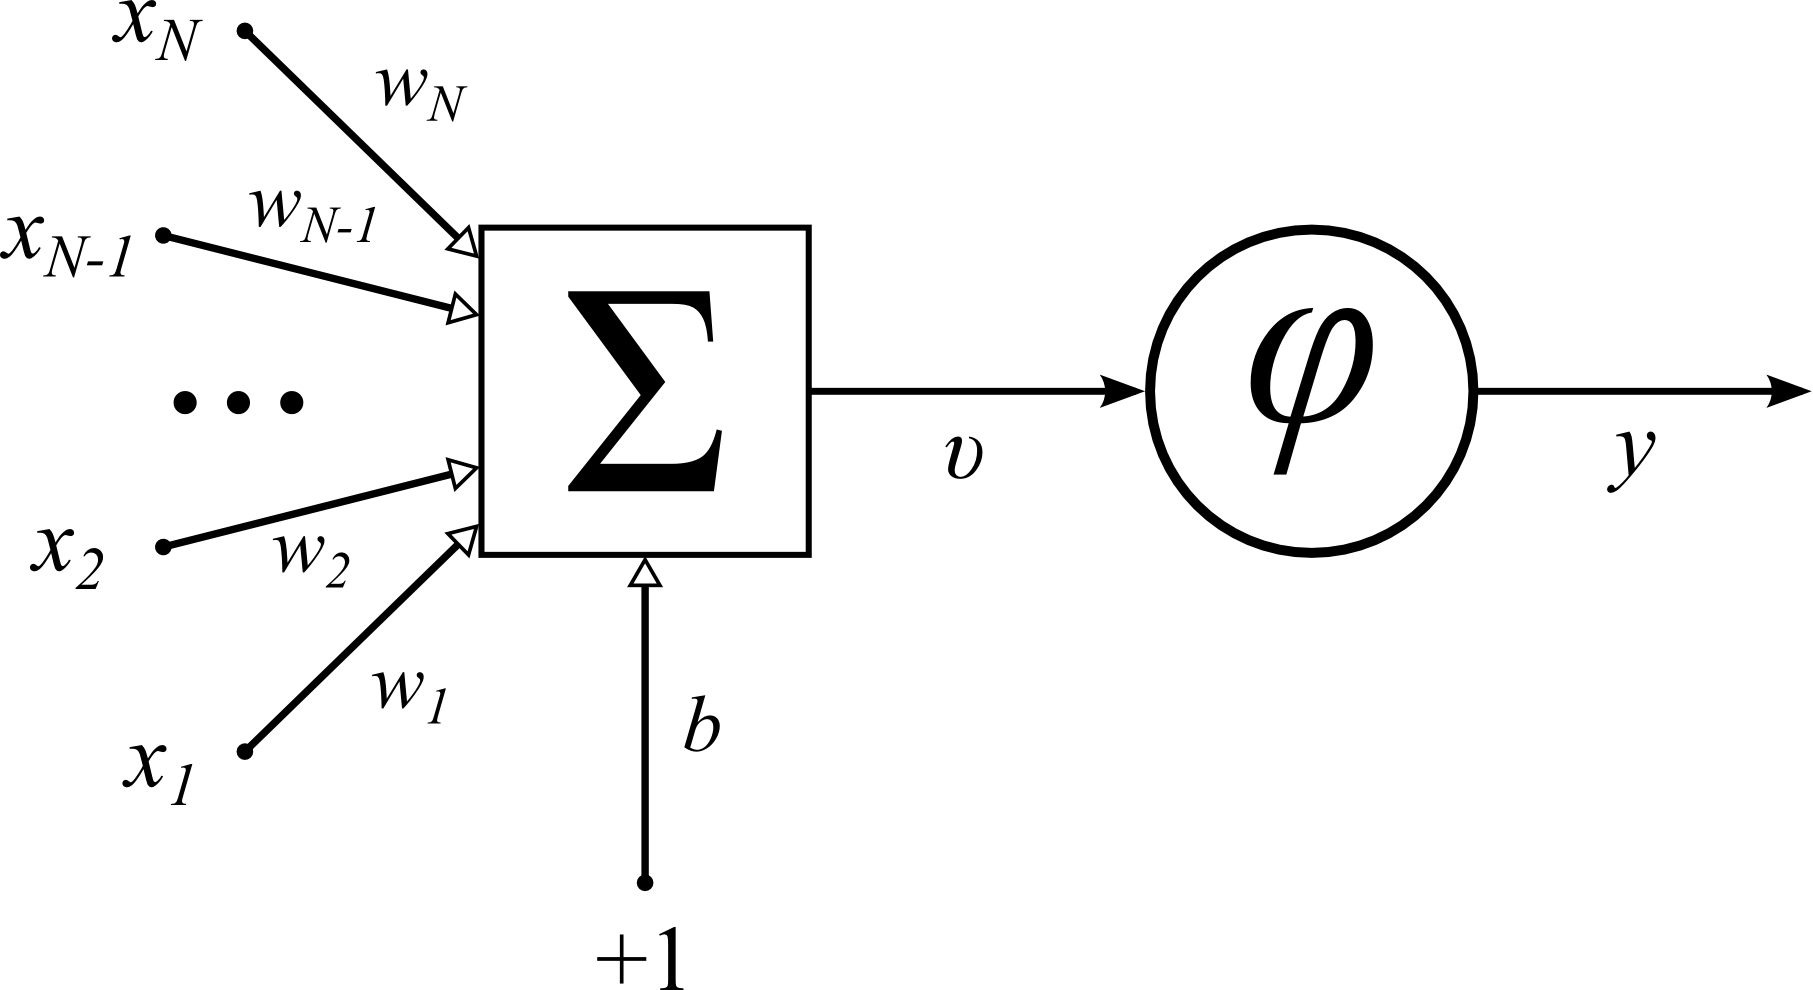
\includegraphics[width=11cm]{artificalNeuron.png}
	\caption{Схематическое представление искусственного нейрона}
	\label{fig:artificalNeuron}
\end{figure}

Математически эту модель можно записать в виде: $y = \phi( \sum_{i=1}^N w_i x_i + b)$.
В настоящее время чаще всего используется сигмоидальная функция активации, которая определяется как $\phi(\nu) = 1 / (1 + e^{-\alpha \nu})$, где $\alpha$ --- некоторый параметр, оптимальное значение которого находится эмпирически.

% мнослойный персептрон
Одной из самых простых моделей искусственных нейронных сетей является простая нейронная сеть с несколькими скрытыми слоями.
Такая нейронная сеть состоит из множества входных узлов, образующих входной слой, одного или нескольких скрытых слоев вычислительных нейронов и одного выходного слоя нейронов.
В такой сети каждый нейрон одного слоя соединён со всеми нейронами предыдущего и последующего слоёв.
Слой, состоящий из таких нейронов, называется полностью связанным слоем.
Входной сигнал распространяется по сети в прямом направлении, от слоя к слою без обратных связей, поэтому такая сеть является нейронной сетью прямого распространения или статической сетью.
Простые нейронные сети с несколькими скрытыми слоями могут применяться для решения широкого круга сложных задач.

Нейронные сети имеют возможность обучаться, в чем и заключается одно из главных их преимуществ перед традиционными методами \cite{nikolenko2017}.
Здесь обучение с учителем выполняется с помощью алгоритма обратного распространения ошибки, который является частным случаем алгоритма минимизации среднеквадратичной ошибки для случая отдельного линейного нейрона.
С математической точки зрения процесс обучения представляет собой нахождение оптимальных весовых коэффициентов, связывающих нейроны.
Лучше, если каждый уровень сети имеет определённый смысл.
Пример такого смыслового разделения представлен на рисунке \ref{fig:staticNeuronNetwork}.

\begin{figure}[h]
	\centering
	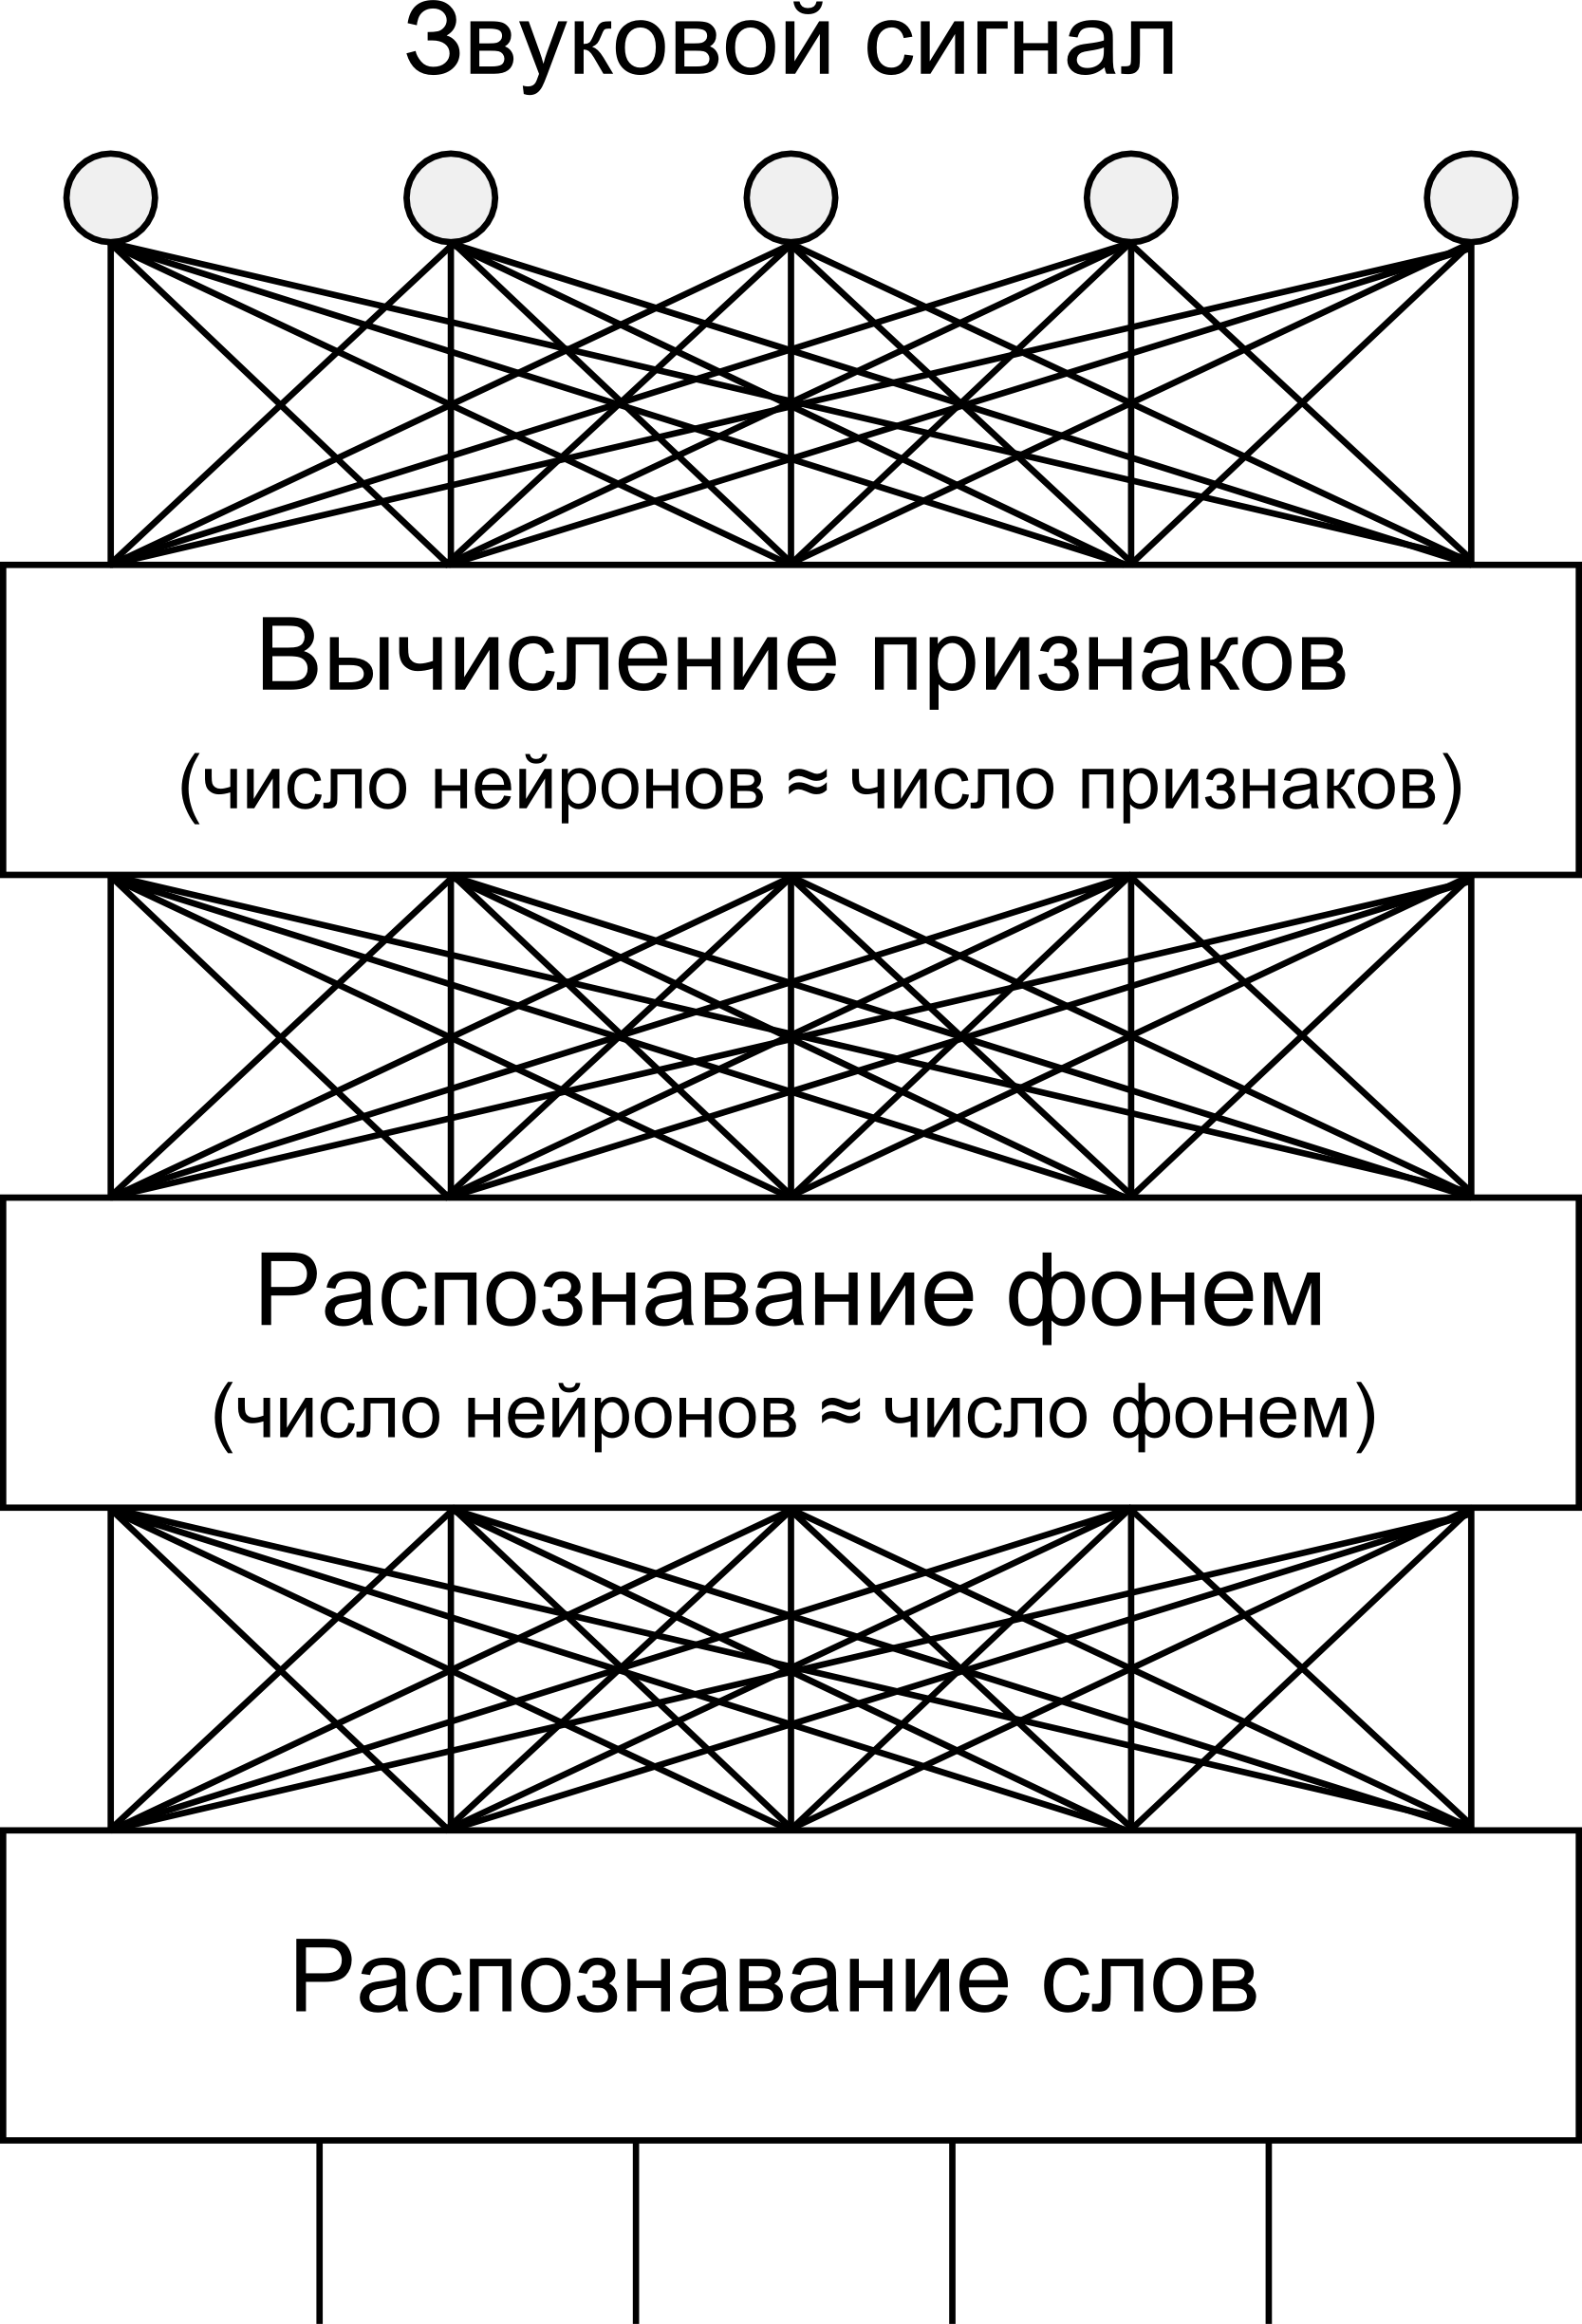
\includegraphics[width=9cm]{staticNeuronNetwork.png}
	\caption{Нейронная сеть прямого распространения с логически разделёнными уровнями}
	\label{fig:staticNeuronNetwork}
\end{figure}

% TDNN
В задачах распознавания речи также применяются искусственные нейронные сети с временными задержками или Time Delay Neural Network (TDNN).

По структуре они являются многослойной нейронной сетью прямого распространения.
Узлы данной сети также содержат временные задержки, что является главной особенностью данного типа искусственных нейронных сетей \cite{waibel1995phoneme}.
Пример внутреннего строения узла с $N$ задержками показан на рисунке \ref{fig:tdnnNode}.

\begin{figure}[h]
	\centering
	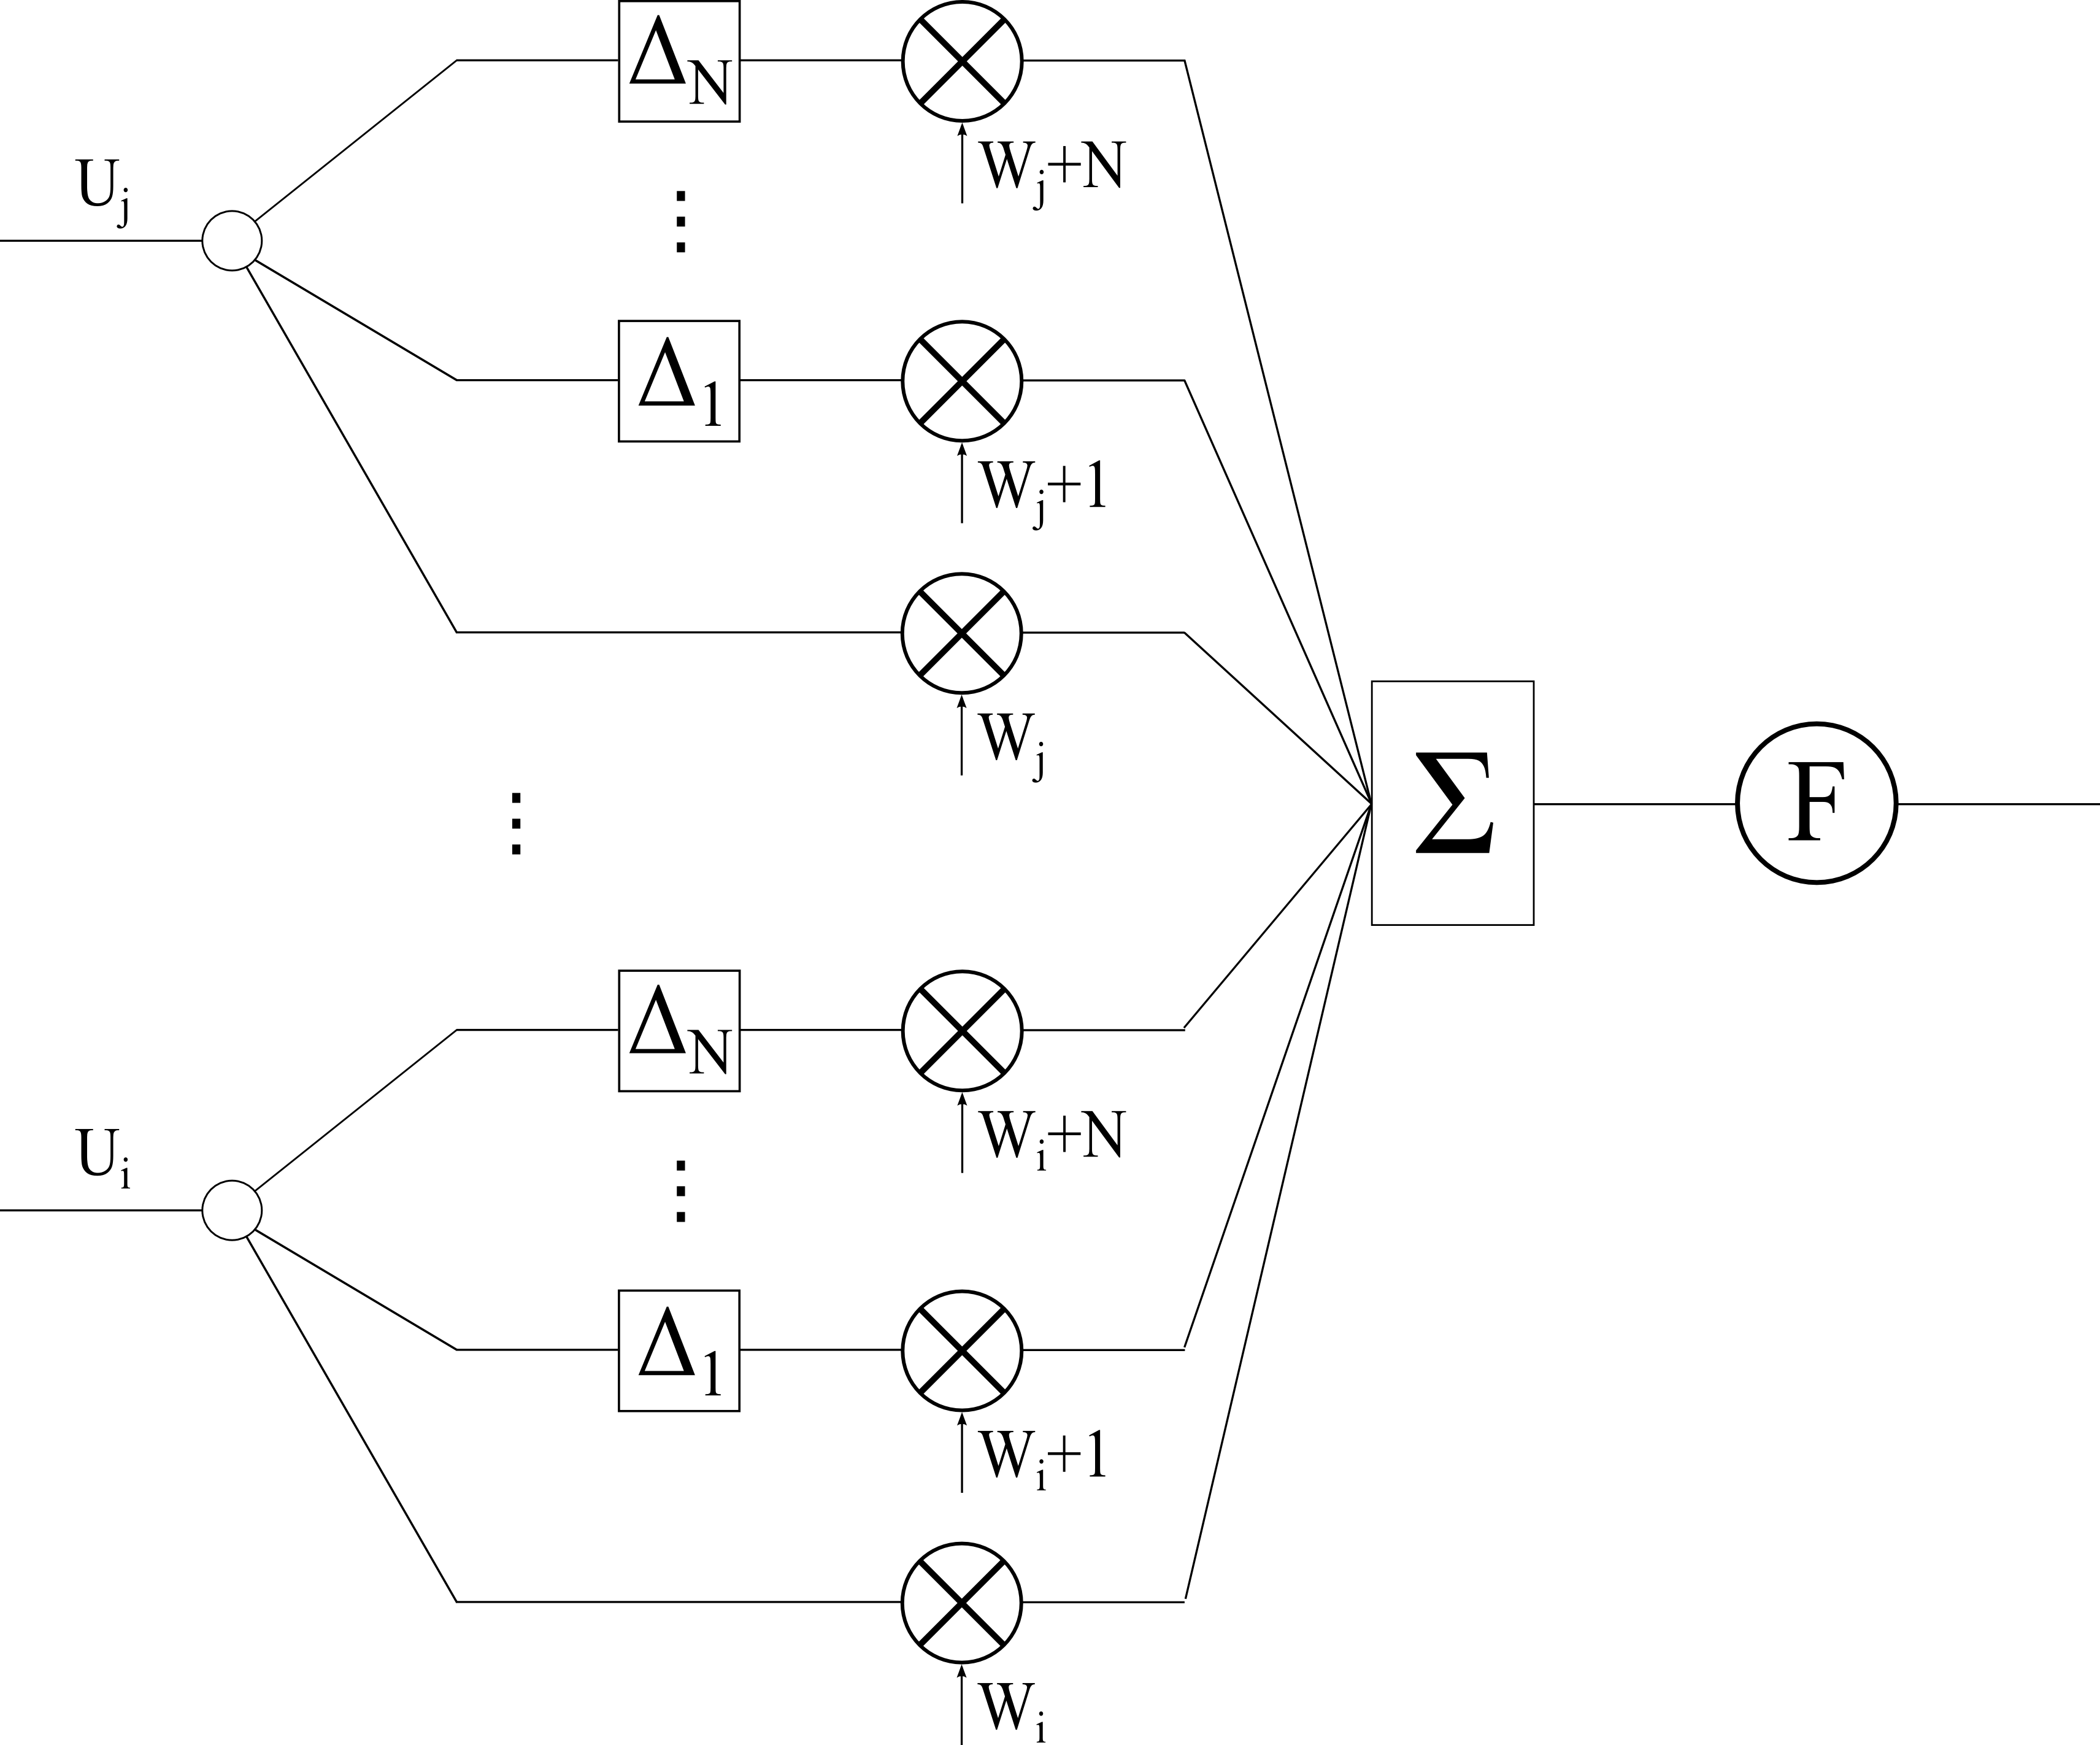
\includegraphics[width=12cm]{tdnnNode.png}
	\caption{Архитектура узла нейронной сети с временными задержками}
	\label{fig:tdnnNode}
\end{figure}

Входные узлы обозначены как $X_1, \dots, X_n$, далее к каждому входному значению применяется $k$ различных смещений $\Delta_1, \dots, \Delta_k$, величина которых выбирается из специфики решаемой задачи.
Таким образом, в TDNN встраивается кратковременная память.
После применения смещений полученные значения умножаются на соответствующие весовые коэффициенты $w_i^j$, в общем случае различные, где $i = \overline{1, n}$ и $j = \overline{1, k}$.
Далее в элементе $\Sigma$ производится суммирование всех слагаемых и затем применяется функция активации $F$.

В качестве примера использования нейронной сети с временными задержками можно рассмотреть задачу распознавания трёх фонем.
Структура сети для решения такой задаче приведена на рисунке \ref{fig:tdnnNetwork}.

\begin{figure}[h]
	\centering
	\includegraphics[width=10cm]{tdnnNetwork.png}
	\caption{Структура нейронной сети с временными задержками}
	\label{fig:tdnnNetwork}
\end{figure}

Из рисунка видно, что обработка входного параметрического портрета представляет собой прохождение входными узлами нейронной сети всего портрета от начала до конца с помощью скользящего по времени окна.
Узлы скрытых слоев сети эквивалентны скользящим детекторам признаков и способны находить искомые образы в любой области входных данных.
Выходные узлы имеют равные веса связей с каждым временным моментом последнего скрытого слоя, поэтому все моменты времени для таких детекторов являются равноправными.
Это позволяет нейронной сети быть инвариантной к временным сдвигам распознаваемых и эталонных образцов фонем, если эти временные сдвиги меньше размера входной последовательности сети.
Данные факты наряду с простой структурой сети дают возможность TDNN быть подходящим инструментом для распознавания речевых сигналов.

% LSTM
Ещё одним типом искусственных нейронных сетей, используемых для распознавания речи, является нейронная сеть с долгой краткосрочной памятью или Long Short-Term Memory (LSTM) \cite{hochreiter1997long}.
Данная архитектура является разновидностью рекуррентных нейронных сетей или Recurrent neural network (RNN).

У обычных нейронных сетей есть серьёзный недостаток --- они не умеют накапливать информацию о предыдущих события, а рекуррентные нейронные сети решают данную проблему.
В них присутствуют сохраняющие информацию циклы, другими словами блоки имеют связи сами с собой.
Из-за присутствия таких циклов рекуррентные сети выглядят довольно необычно и запутанно, но каждый цикл можно представить как несколько копий одного и того же блока.
Развёртка показана на рисунке \ref{fig:rnnBlock}, где видно, что развёрнутая сеть уже больше похожа на традиционные нейронные сети.

\begin{figure}[h]
	\centering
	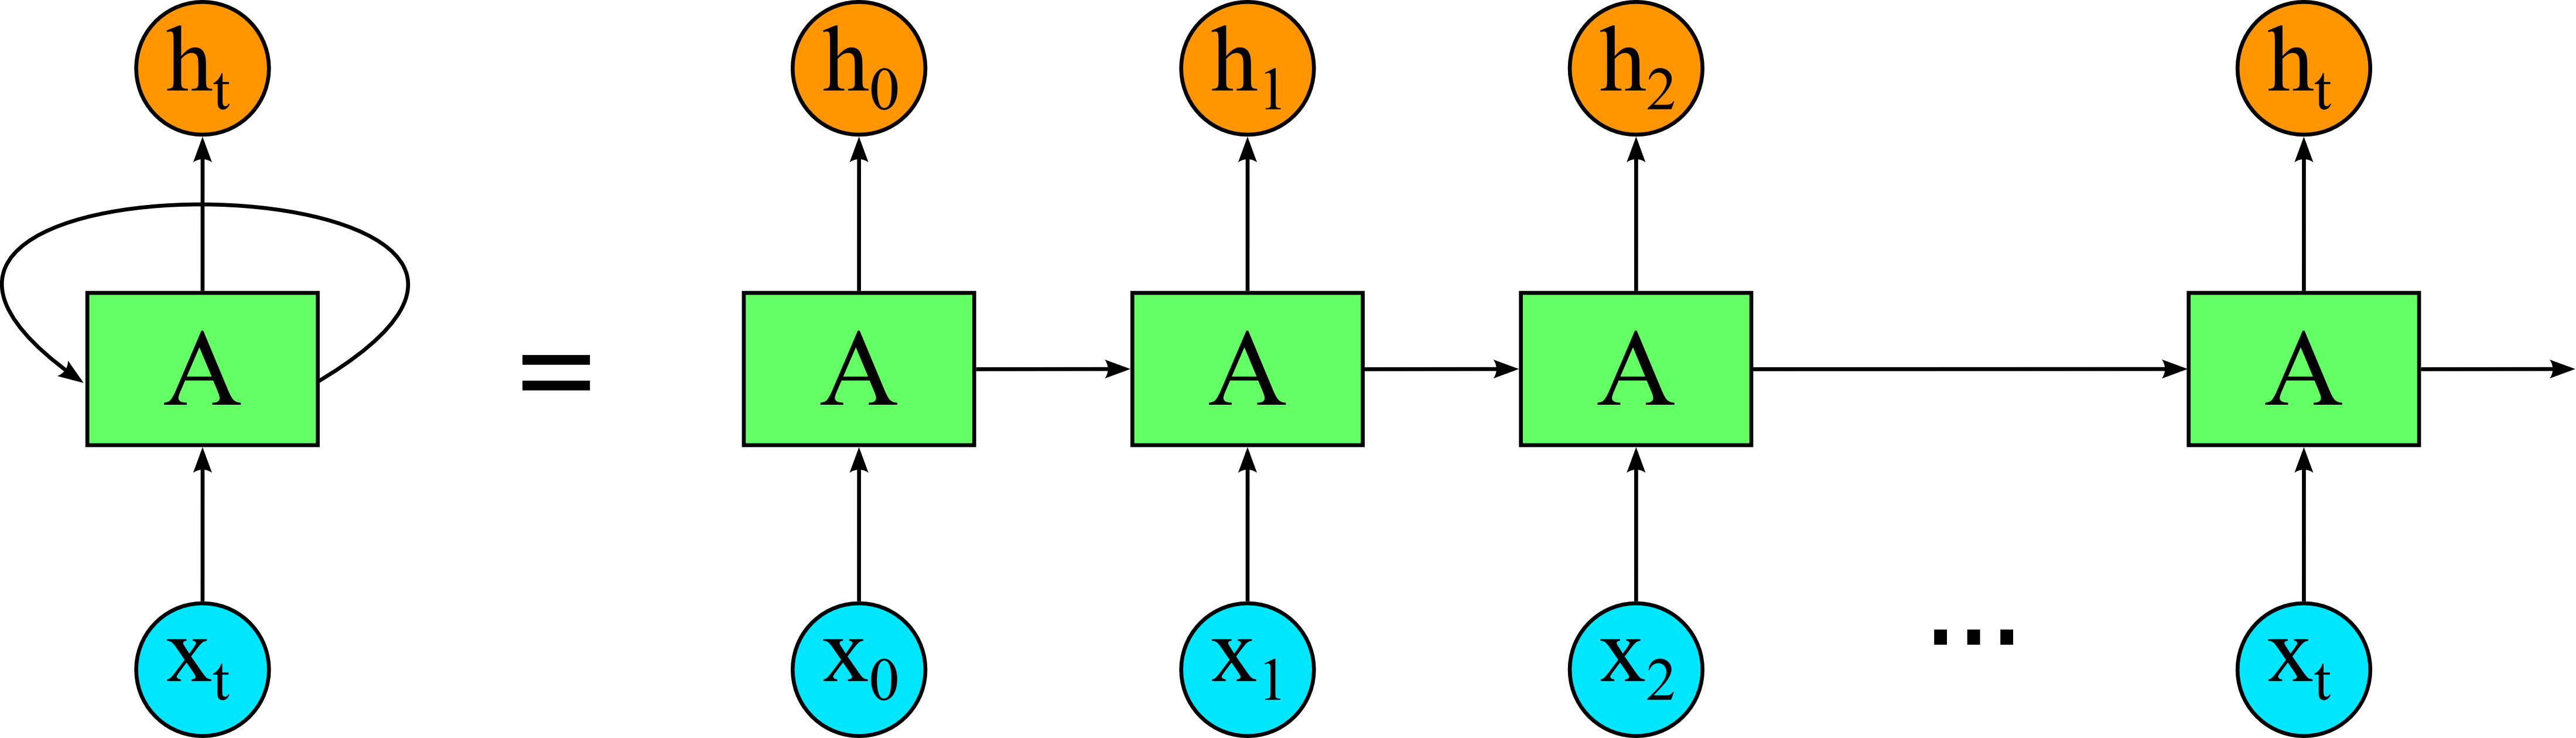
\includegraphics[width=16cm]{rnnBlock.png}
	\caption{Развёртка цикла рекуррентной нейронной сети}
	\label{fig:rnnBlock}
\end{figure}

Проблема RNN заключает в том, что она быстро <<забывает>> информацию, то есть с трудом строит долгосрочные зависимости между информацией в начале и в конце сигнала.
Нейронные сети c долгой краткосрочной памятью, как следует из их названия, были созданы как раз для решения данной проблемы.
Отличие LSTM от обычных RNN заключается в структуре блоков.
Блок стандартной рекуррентной сети как правило простой, например, один слой функции гиперболического тангенса.

LSTM-блоки обычно содержат 3 <<вентиля>>, которые используются для контроля потоков информации на входах и на выходах памяти блоков.
Блок с 3 вентилями: входным, выходным и вентилем забывания, приведён на рисунке \ref{fig:lstmBlock}.

\begin{figure}[h]
	\centering
	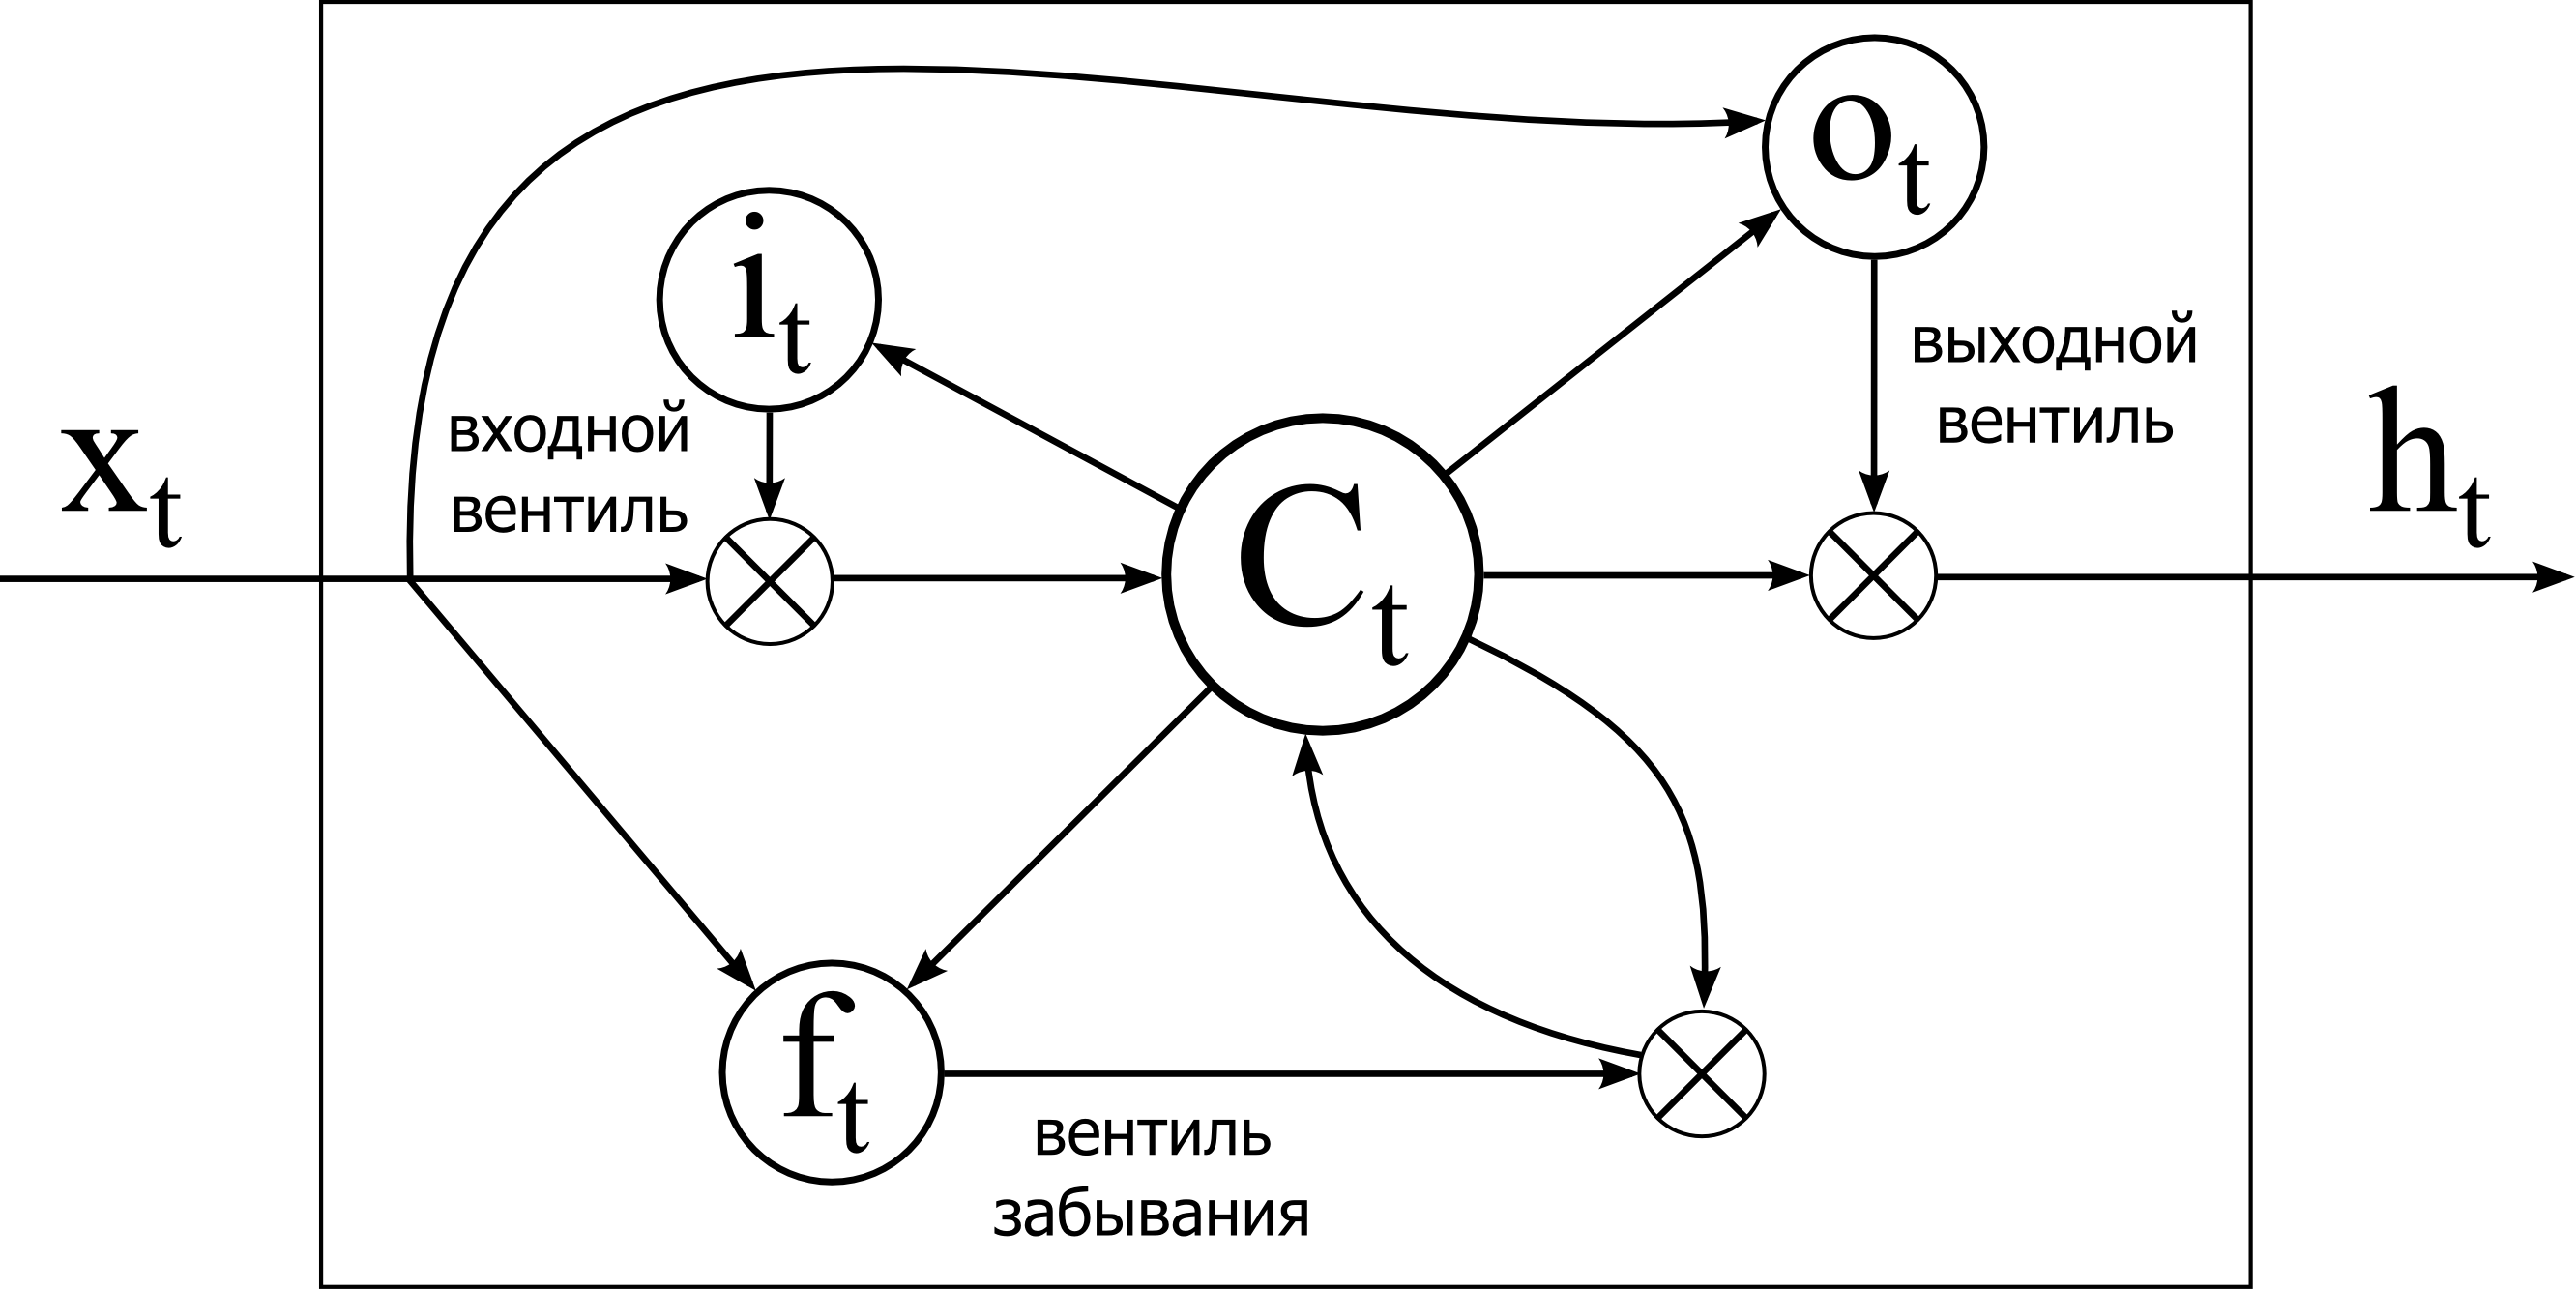
\includegraphics[width=14cm]{lstmBlock.png}
	\caption{Структура LSTM-блока с 3 вентилями}
	\label{fig:lstmBlock}
\end{figure}

Вентили реализованы в виде логистической функции для вычисления значения в диапазоне $[0, 1]$ и имеют в параметрах веса, которые подбираются в процессе обучения методом обратного распространения ошибки.
Умножение на это значение используется для частичного допуска или запрещения потока информации внутрь и наружу памяти.
Основная идея заключается в том, что старое значение следует забывать только тогда, когда появится новое значение достойное запоминания.

% сверточные нейронные сети
Другим классом искусственных нейронных сетей являются глубокие нейронные сети --- это нейронные сети прямого распространения с большим числом скрытых слоёв.
Одним из примеров глубоких нейронных сетей являются CNN (convolutional neural network, нейронные сети на основе свёртки), использующиеся при анализе изображений, распознавании речи и в других задачах \cite{lecun1995convolutional, abdel2014convolutional}.
В головном мозге человека были обнаружены клетки, имеющие различную функциональную нагрузку \cite{matsugu2003subject}.
Среди них были как простые клетки, которые реагировали на прямые линии, расположенные под различными углами, так и сложные клетки, которые активировались только при условии активации нескольких простых клеток.
Описанные выше искусственные нейронные сети как раз используют данное разделение функций между нейронами.
Общая схема работы CNN, описанная далее, показана на рисунке \ref{fig:cnn_typical}.

\begin{figure}[h]
	\centering
	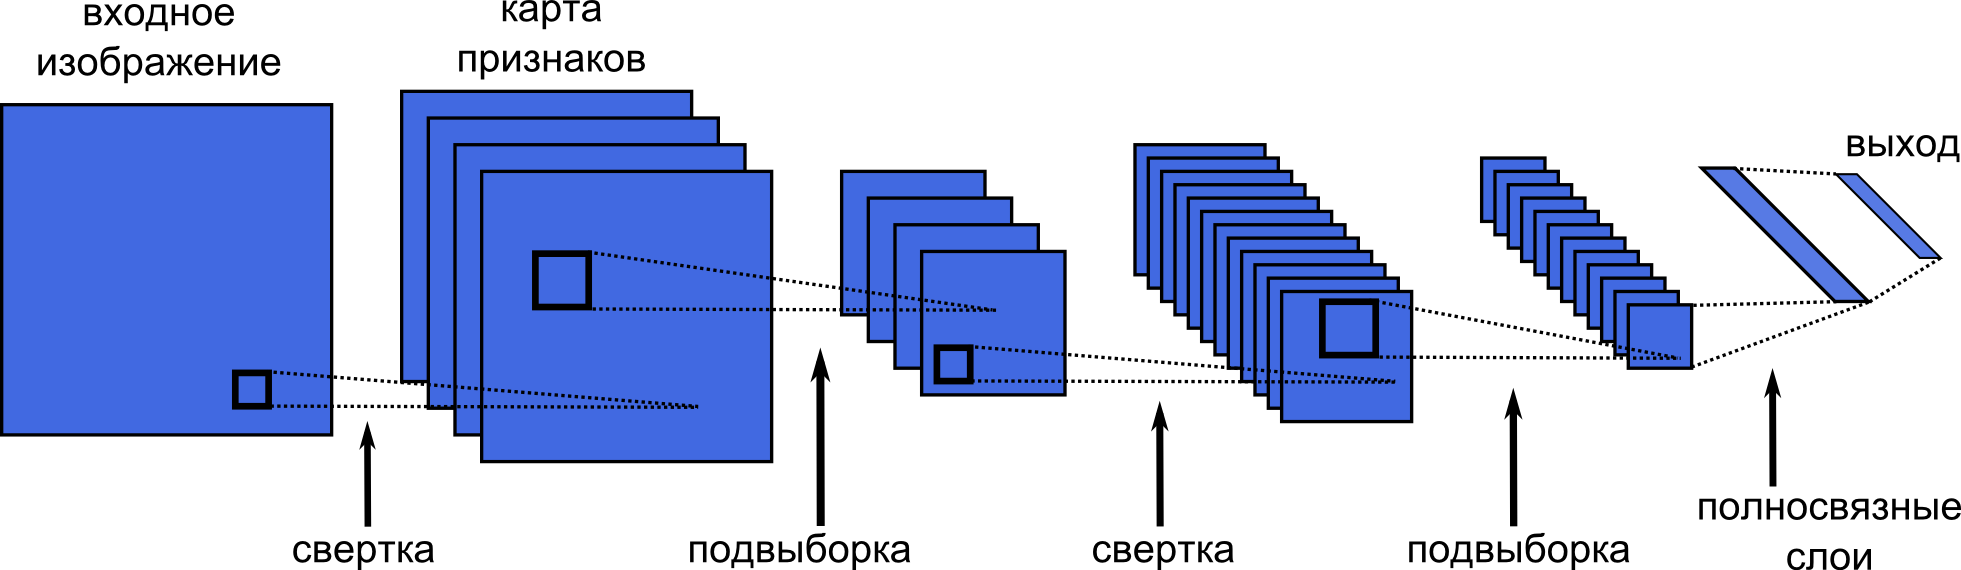
\includegraphics[width=1.0\textwidth]{cnn_typical.png}
	\caption{Общая схема работы CNN}
	\label{fig:cnn_typical}
\end{figure}

Так как изначально они были предложены для распознавания изображений, на вход подаётся один двухмерный массив (для черно-белых изображений) или несколько двухмерных массивов (для цветных изображений).
Такой формат входных данных отлично подходит для распознавания речи, так как в нём в качестве исходных данных также используется двухмерный параметрический портрет.
Входные массивы, также как и промежуточные массивы, называются картами признаков.

Далее вместо полностью связанных скрытых слоев используется другая структура сети, состоящая из чередующихся слоев свёртки и выборки.
На рисунке \ref{fig:convolution_pooling} приведено наглядное представление операции свёртки и операции выборки.

\begin{figure}[h]
	\centering
	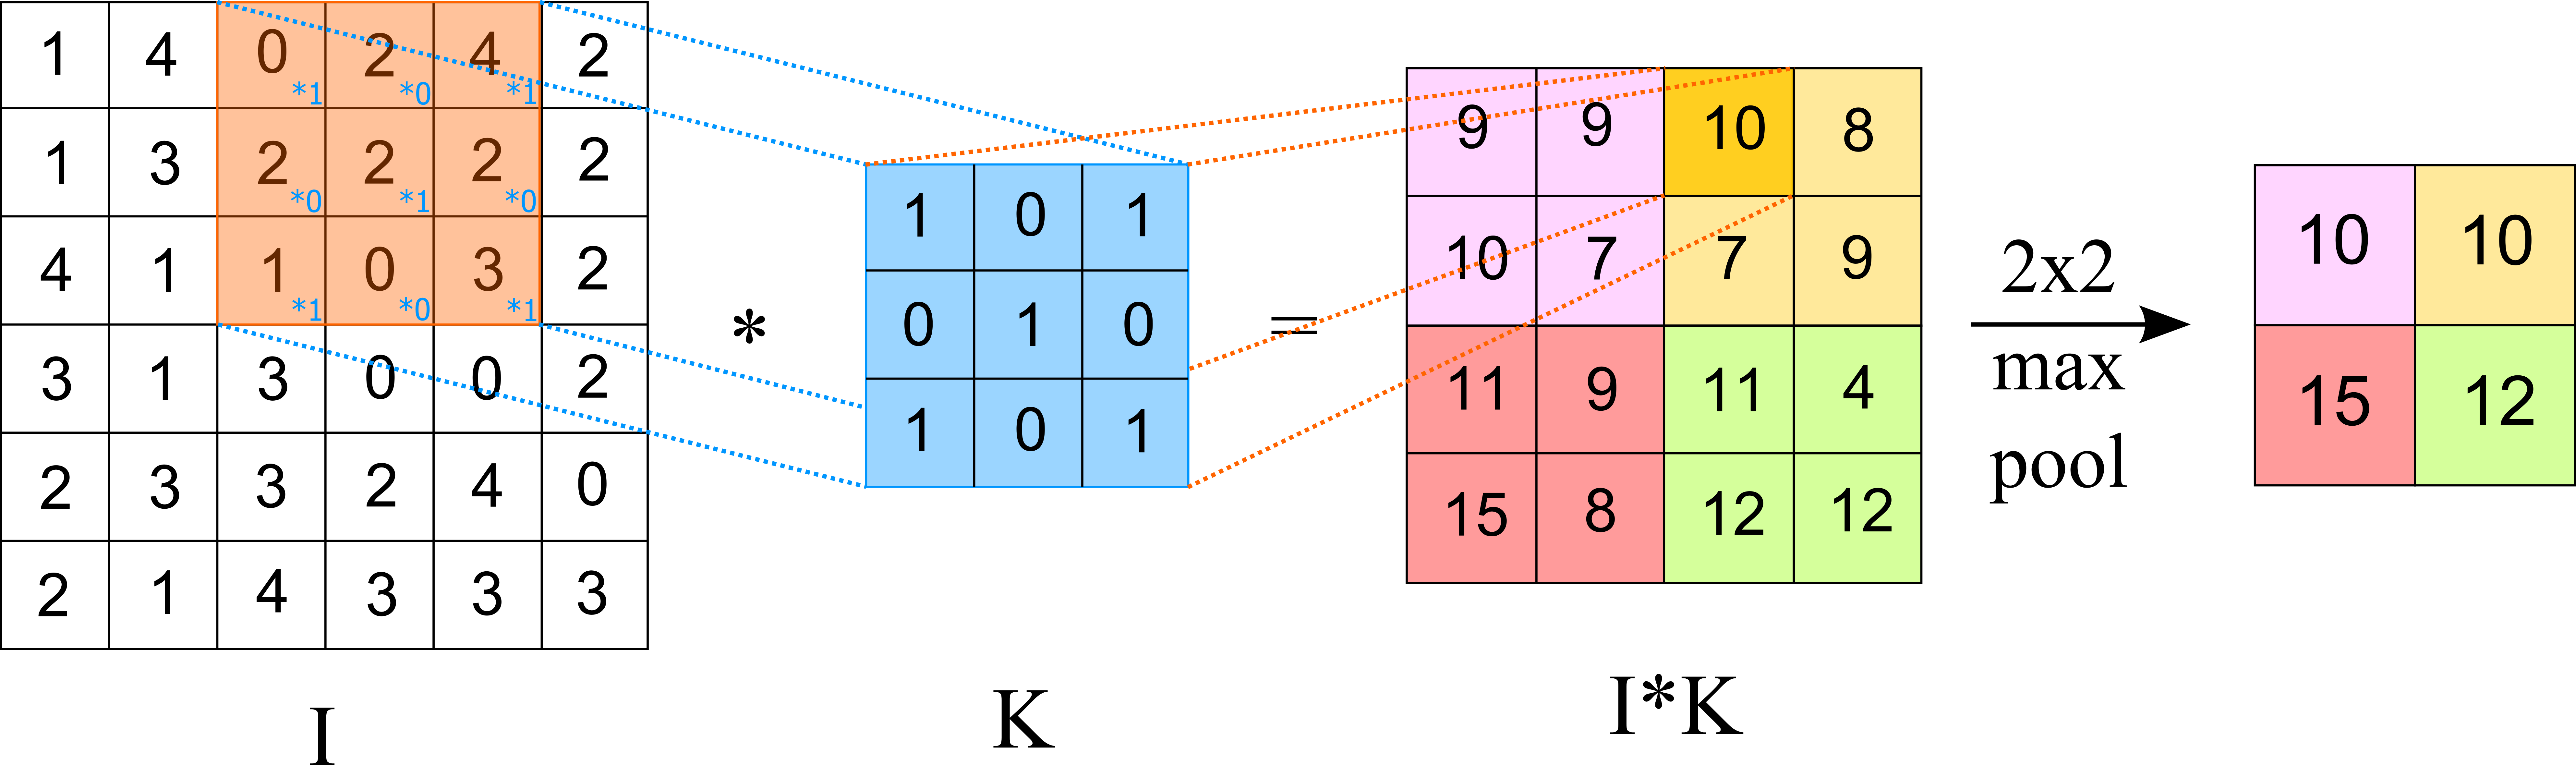
\includegraphics[width=1.0\textwidth]{convolution_pooling.png}
	\caption{Схема работы слоев свёртки и выборки в CNN}
	\label{fig:convolution_pooling}
\end{figure}

В операции свёртки каждый фрагмент карты признаков умножается на некоторую матрицу свёртки (ядро) поэлементно, а результат суммируется и записывается в соответствующую позицию выходной карты признаков.
В каждом слое может применяться набор из нескольких матриц сверки, при этом проход каждым из фильтров создаёт уникальную карту признаков.
Это делает искусственную нейронную сеть многоканальной, то есть имеется набор независимых карт признаков в каждом слое.
Операция выборки производит уменьшение размерности сформированных карт признаков, позволяя ускорить дальнейшие вычисления и обеспечить инвариантность к масштабу входного сигнала.

По мере прохождения слоев свёртки и выборки, карта признаков уменьшается в размере, но увеличивается количество каналов.
Далее, после прохождения всех слоев карта представляется в виде скаляра или вектора, но количество её каналов достигает нескольких десятков, сотен или даже тысяч.
На выходе нейронной сети дополнительно устанавливают один или несколько полностью связанных слоёв, на вход которым подаются все каналы из карты признаков.

Стандартным методом, используемым при обучении искусственных нейронных сетей, является алгоритм обратного распространения ошибки.
Также может быть использована любая функция активации нейронов.

%\newpage
%============================================================================================================================

\section{Обзор используемых в работе математических алгоритмов} \label{sect1_4}

В данном подразделе будут рассмотрены математические методы, используемые далее в предложенных алгоритмах.

%\newpage
%============================================================================================================================

\subsection{Методы математической статистики, необходимые для анализа свойств речевых сигналов} \label{sect1_4_1}

Существует несколько критериев согласия для проверки законов распределения случайной величины.
Это критерии согласия Колмогорова, Смирнова, $\chi^2$ Пирсона и другие.
В данной работе для проверки статистических гипотез будет использоваться критерий Пирсона, как один из наиболее часто употребляемых и широко описанных в литературе критериев для проверки закона распределения случайной величины \cite{panteleev2001}.

\textbf{Формирование критерия оценивания качества распознавания}

Сравнение распознаваемого слова с эталоном можно осуществить по критерию максимума коэффициента корреляции, оценка которого вычисляется по формуле 

\begin{equation}
\widehat{\rho}_{xe} = \frac{\sum_{n=1}^{N_s} (x_n - \widehat{m}_x)(e_n - \widehat{m}_e)}{\sqrt{\sum_{n=1}^{N_s} (x_n - \widehat{m}_x)^2 \sum_{n=1}^{N_s} (e_n - \widehat{m}_e)^2}},
\end{equation}
\begin{itemize}[align=left,leftmargin=1.8em,itemindent=0pt,labelsep=0pt,labelwidth=1.8em]
	\item[где] $x_n$, $e_n$, $n = 1, 2, \dots, N_s$ --- элементы матриц параметрического портрета рассматриваемого слова и эталона, преобразованные в одномерные массивы размерности $N_s = N_t N_f$;
	\item[] $\widehat{m}_x$, $\widehat{m}_e$ --- оценки средних параметрического портрета слова и эталона, вычисленные по множеству всех элементов, то есть 
	$\widehat{m}_x = \frac{1}{N_s} \sum_{n=1}^{N_s} x_n$, $\widehat{m}_e = \frac{1}{N_s} \sum_{n=1}^{N_s} e_n$.
\end{itemize}

При проверке гипотез и построении доверительных интервалов для коэффициентов корреляции часто используется Z-преобразование Фишера $z(\widehat{\rho}) = \frac{1}{2} \ln\left(\frac{1+\widehat{\rho}}{1-\widehat{\rho}}\right)$, где $\widehat{\rho}$ --- выборочный коэффициент корреляции.
Это преобразование даёт величину, распределение которой приближается к нормальному с математическим ожиданием $M[z] = \frac{1}{2} \ln\left(\frac{1+\rho}{1-\rho}\right)$ и дисперсией $D[z] = \frac{1}{n-3}$, где $n$ --- длина выборки, $\rho$ --- истинное значение коэффициента корреляции.

Далее в работе при сравнении двух параметрических портретов будет применяться именно Z-преобразование Фишера.

%============================================================================================================================

\subsection{Подстройка по длительности и динамическое программирование} \label{sect1_4_2}

При распознавании речевых команд путём сравнения их с эталонами требуется приведение временных масштабов двух сравниваемых слов в оптимальное соответствие.
Эффективное решение данной проблемы лежит в алгоритмах динамического программирования.
Алгоритмы такого типа являются динамическими алгоритмами трансформации временной шкалы.
Далее будет представлено описание работы данного алгоритма при распознавании отдельных слов.

Алгоритм динамической трансформации времени (ДТВ) основан на динамическом программировании.
Он вычисляет оптимальную последовательность трансформации времени между двумя временными рядами \cite{lama2010speech}.

Рассмотрим 2 последовательности векторов признаков различной длины: $A = \{a_1, a_2, \dots, a_i, \dots, a_n\}$ и $B = \{b_1, b_2, \dots, b_j, \dots, b_m\}$.
Допустим, что последовательность $A$ является эталоном, а последовательность $B$ --- входным словом.

Для начала рассчитаем величины локальных отклонений между элементами двух последовательностей.
Самым распространённым методом вычисления расстояния является расчёт абсолютного отклонения между значениями пары элементов.
В результате получится матрица расстояний, имеющая $m$ строк и $n$ столбцов общих членов: $dist_{ij} = |a_i - b_j|$, $i = \overline{1, n}$, $j = \overline{1, m}$.

Алгоритм динамического программирования определяется тем наблюдением, что в двумерной матрице наиболее оптимальный маршрут к точке $(i, j)$ должен быть проложен через точку $(i-1, j)$, или $(i-1, j-1)$, или $(i, j-1)$, как показано на рисунке \ref{fig:dynamicProgrammingPaths}.

\begin{figure}[h]
	\centering
	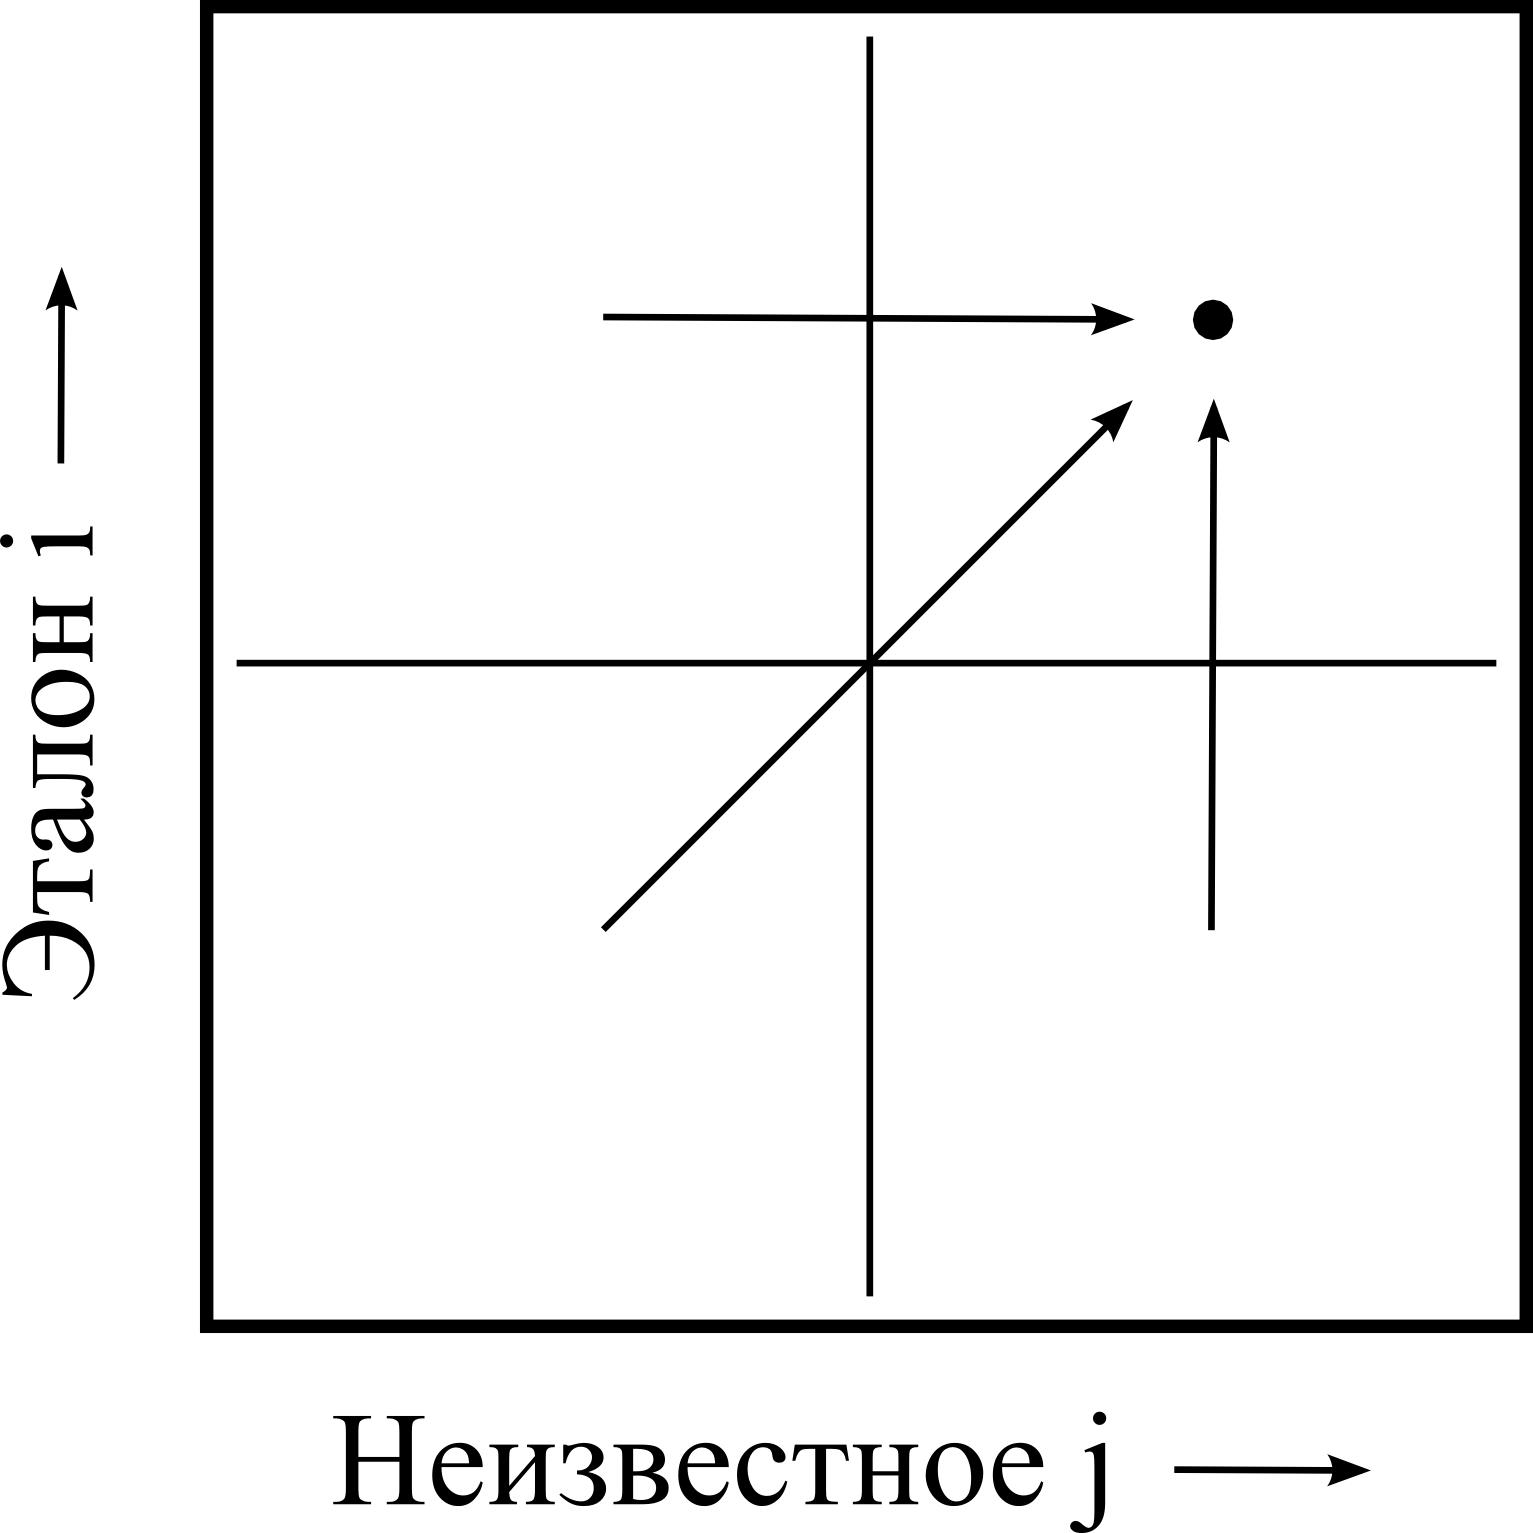
\includegraphics[width=6cm]{dynamicProgrammingPaths.png}
	\caption{Возможные варианты пути к $(i, j)$ в двумерной матрице}
	\label{fig:dynamicProgrammingPaths}
\end{figure}

Поэтому общий минимальный путь к точке $(i, j)$ определяется соотношением
\begin{equation}
D(i, j) = dist_{ij} + \min\{D(i-1, j); D(i-1, j-1); D(i, j-1)\},
\end{equation}
где $D(i, j)$ --- суммарное расстояние от точки $(1, 1)$ до точки $(i, j)$, а $dist_{ij}$ --- локальное расстояние (отклонение) в точке $(i, j)$, заданное выше.
\begin{itemize}[align=left,leftmargin=1.8em,itemindent=0pt,labelsep=0pt,labelwidth=1.8em]
	\item[где] $D(i, j)$ --- суммарное расстояние от точки $(1, 1)$ до точки $(i, j)$,
	\item[] $dist_{ij}$ --- локальное расстояние (отклонение) в точке $(i, j)$, заданное выше.
\end{itemize}

Длина пути от одной точки до следующей измеряется акустической аналогичностью эталона и неизвестного входного сигнала в этой точке.

Алгоритм рекурсивно вычисляет это расстояние элемент за элементом, чтобы определить минимальное суммарное расстояние $D(n, m)$ от начальной точки $(1, 1)$ до точки $(n, m)$ в верхнем правом углу.
Описанный путь позволяет получить временное выравнивание, в результате которого эталон становится максимально похож акустически на слово, которое было на входе.

На рисунке \ref{fig:dynamicProgrammingExample} схематически представлено выравнивание двух последовательностей на простом примере \cite{lea1980trends, gawali2010marathi}.

\begin{figure}[h]
	\centering
	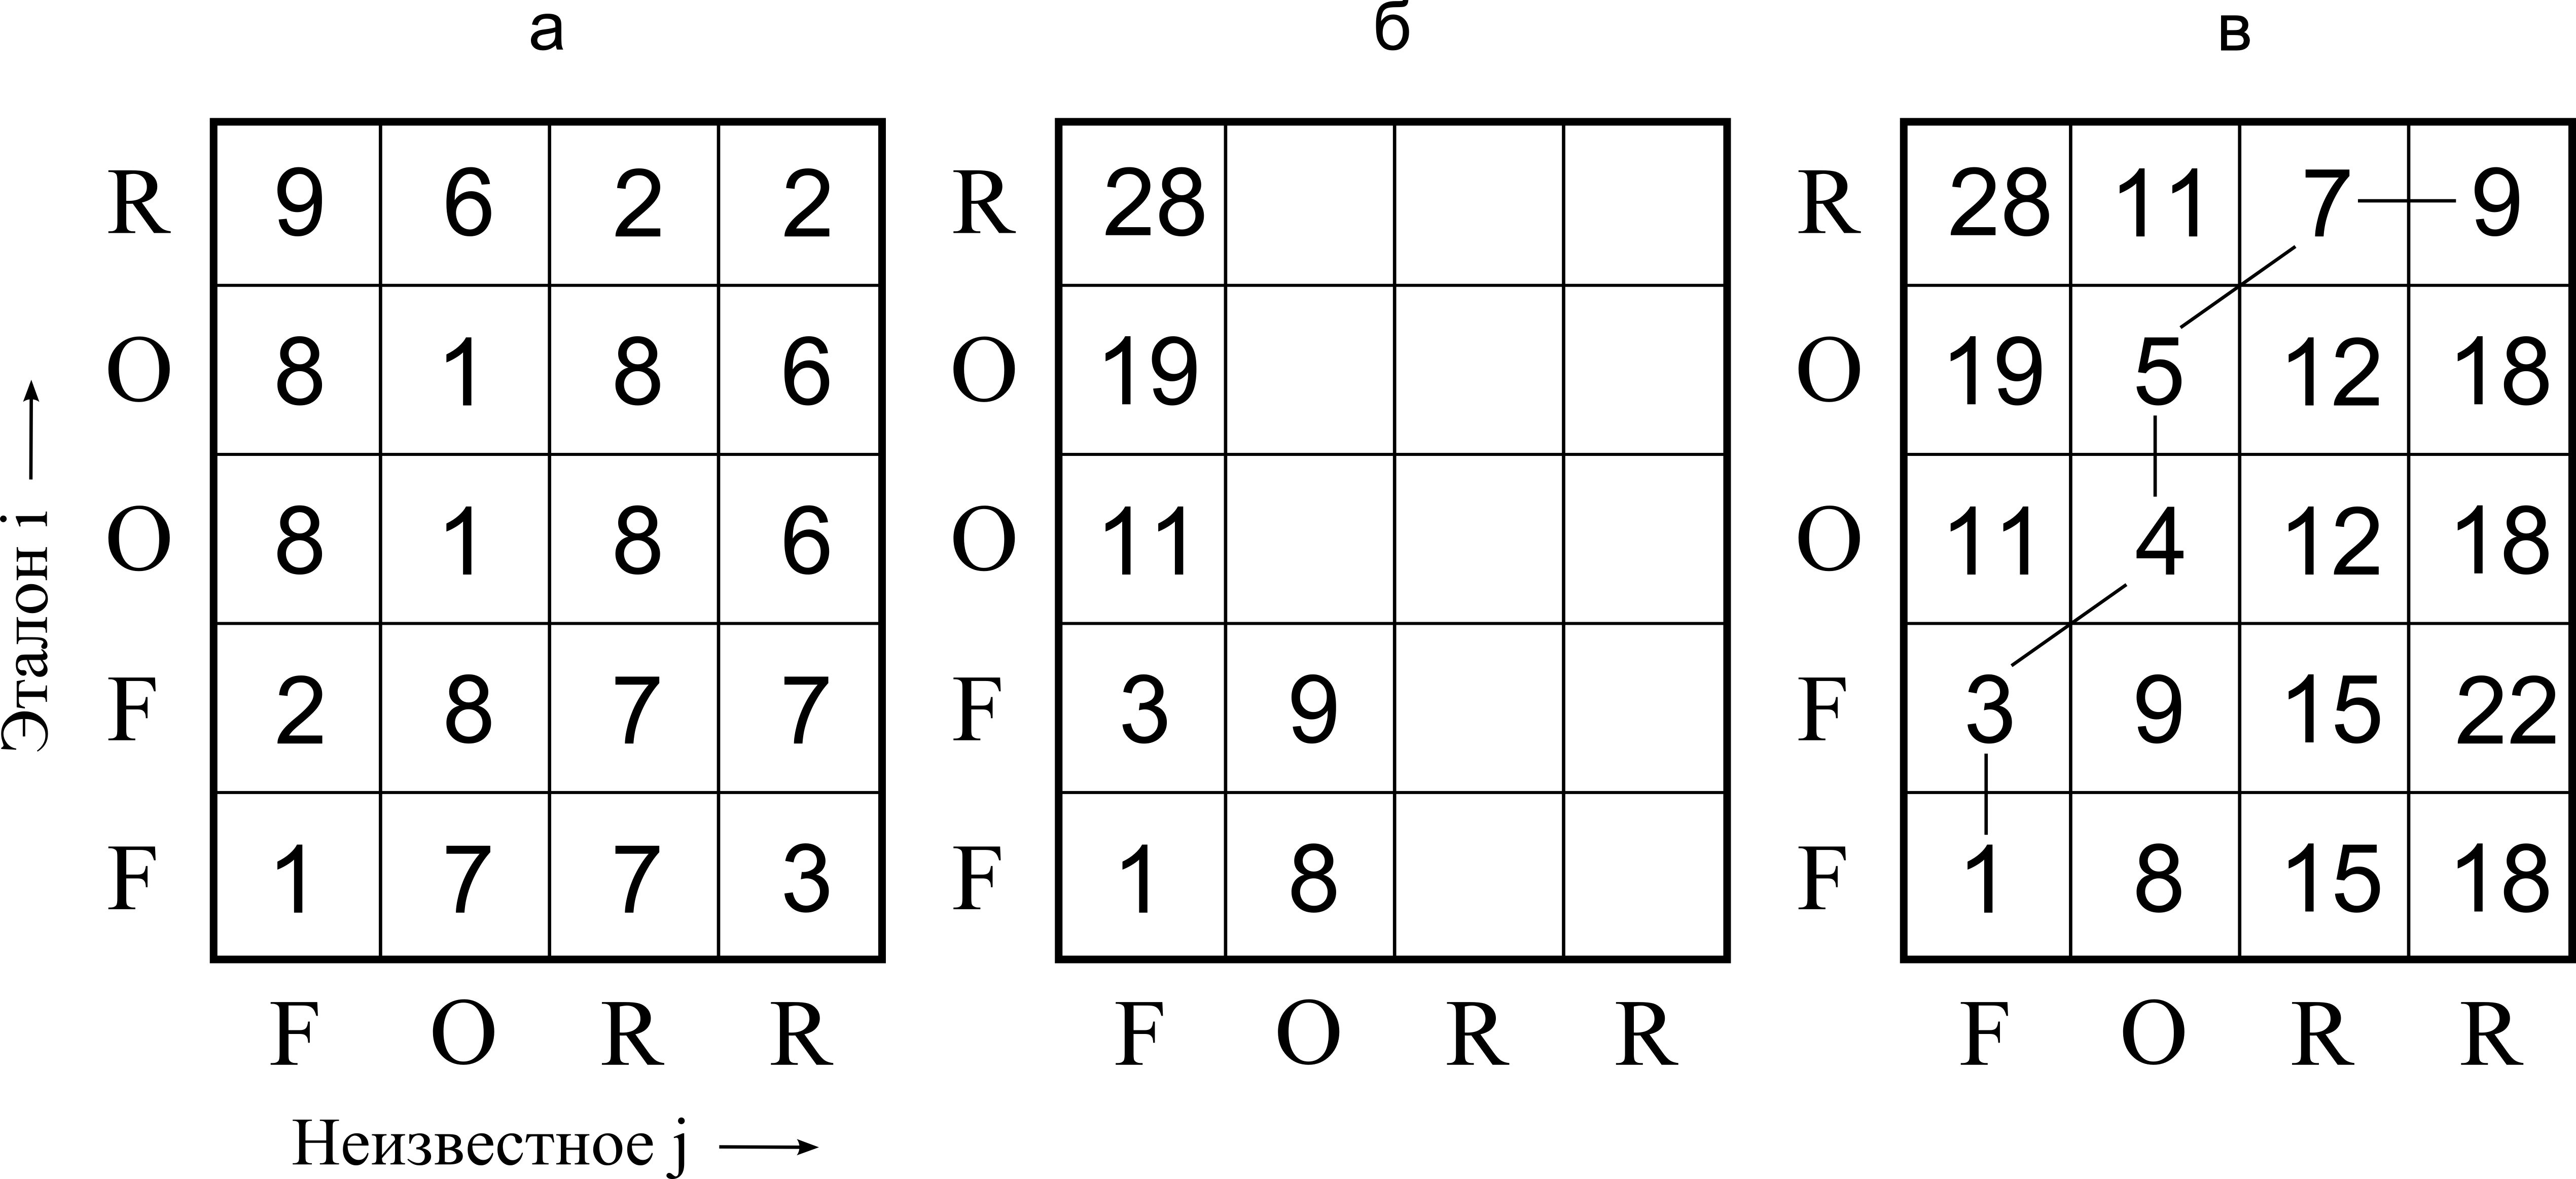
\includegraphics[width=16cm]{dynamicProgrammingExample.png}
	\caption{Пример динамического программирования: а) матрица подобия речевых звуков эталона и неизвестного сигнала; б) вычисление минимального общего расстояния до каждой точки по столбцам; в) окончательная матрица с общим совокупным расстоянием, равным 9}
	\label{fig:dynamicProgrammingExample}
\end{figure}

Длина последовательности эталона FFOOR равна $m = 5$, а длина распознаваемого слова FORR --- $n = 4$.
В первой части рисунка представлена матрица подобия элементов речевых сигналов эталона и распознаваемого слова.
В ней видно, что схожие элементы последовательностей имеют маленькие отклонения $dist_{ij}$, а различные элементы --- большие отклонения.
Все возможные пути, начало которых находится в нижнем левом углу и конец в верхнем правом углу дают совокупность возможных выравниваний неизвестного высказывания и соответствующего ему эталона.
Во второй части рисунка показан процесс построения суммарных расстояний $D(i, j)$.
А в третьей части рисунка показана полностью построенная матрица суммарных расстояний $D(i, j)$ и отмечен оптимальный путь до точки $(n, m)$.

В подразделе \ref{sect2_2} следующего раздела будет приведено подробное описание применяемых стандартного и модифицированного алгоритмов динамического программирования.

%\newpage
%============================================================================================================================

\subsection{Метод главных компонент} \label{sect1_4_3}

Для уменьшения размерности пространства используемых векторов без существенной потери информации используется метод главных компонент.
Метод главных компонент используется во многих областях от статистики до медицины \cite{aivazyan1989prikladnaya}.
Главные компоненты представляют собой ортогональную систему координат, в которой дисперсии компонент характеризуют их статистические свойства.

Пусть дан исходный набор векторов $\pmb{X}$ линейного пространства $\pmb{L}^p$.
Использование метода главных компонент даёт возможность перейти к базису пространства $\pmb{L}^{p'}$, $(p' \ll p)$, при котором первый вектор базиса сонаправлен с вектором, вдоль которого максимально значение дисперсии векторов изначального набора векторов.
Направление второго вектора базиса необходимо выбрать так, чтобы максимизировать значение дисперсии базовых векторов, проходящих вдоль него, при соблюдении условия ортогональности относительно первого вектора базиса.
Аналогично определяются остальные векторы базиса.

В итоге для того, чтобы максимально увеличить значение дисперсии изначального набора векторов вдоль первых компонент, называемых главными компонентами, были подобраны соответствующие направления векторов базиса.
Таким образом, основные показатели изменчивости базовых наборов векторов обусловлены характеристиками нескольких первых компонентов, вследствие чего возможно перейти к пространству с меньшей размерностью, исключив менее существенные компоненты \cite{aivazyan1989prikladnaya}.

Пусть имеется многомерное наблюдение $X_i = \begin{pmatrix} x_i^{(1)} \\ x_i^{(2)} \\ \vdots \\ x_i^{(p)} \end{pmatrix}$, $i = \overline{1, n}$.
В итоге, задачей является переход от количества признаков $p$ к $p'$.
Что можно реализовать в случае определения всех возможных нормированных линейных ортогональных комбинаций начальных показателей $z^{(j)}(X) = c_{j1} (x^{(1)} - \mu^{(1)}) + \dots + c_{jp} (x^{(p)} - \mu^{(p)})$, где $[\mu^{(1)}, \dots, \mu^{(p)}]'$ --- вектор средних для переменной $X$.
В качестве меры информативности $p'$-мерной системы показателей $(z^{(1)}(X), \dots, z^{(p')}(X))$ используется выражение $I_{p'}(Z(X)) = \frac{D(z_1) + \dots + D(z_{p'})}{D(x_1) + \dots + D(x_{p})}$, где $D(z)$ --- это операция вычисления дисперсии случайной величины.
Можно продемонстрировать, что соотношение, позволяющее рассчитать $p$ главных компоненты вектора $X$, возможно представить в виде $Z = LX$, где $Z = (z^{(1)}, \dots, z^{(p)})'$, $X = (x^{(1)}, \dots, x^{(p)})'$, а матрица $L$ состоит из строк $l_j = (l_{j1}, \dots, l_{jp})$, $j = \overline{1, p}$, являющихся собственными векторами ковариационной матрицы случайной величины $X$ $\Sigma = \sigma_{ij}$, $i,j = \overline{1, p}$, соответствующими собственным числам $\lambda_j$, $j = \overline{1, p}$.

Основные свойства главных компонент:
\begin{itemize}
	\item матрица $L$ является ортогональной, то есть $L L' = L' L = I$, где $I$ --- единичная матрица; 
	\item ковариационная матрица вектора главных компонент: $\Sigma_{Z} = L \Sigma L' = \begin{pmatrix} \lambda_1 & \dots & 0 \\ \vdots & \ddots & \vdots \\ 0 & \dots & \lambda_p \end{pmatrix}$;
	\item равенство сумм дисперсий исходных признаков и главных компонент;
	\item мера информативности метода $I_{p'}(Z(X)) = \frac{\lambda_1 + \lambda_2 + \dots + \lambda_{p'}}{\lambda_1 + \lambda_2 + \dots + \lambda_p}$, где $\lambda_1, \lambda_2, \dots, \lambda_p$ --- собственные числа ковариационной матрицы $\Sigma$ вектора $X$, расположенные в порядке убывания;
	следует использовать данный критерий для принятия решения о допустимости отбрасывания определённого числа наименее значимых главных компонент без существенного ущерба, с целью уменьшения показателя размерности исследуемого пространства.	
\end{itemize}

%\newpage
%============================================================================================================================

\subsection{Обзор методов численной оптимизации, метод покоординатного спуска} \label{sect1_4_4}

Задачи отыскания наибольших или наименьших величин часто возникают в науке.
Классическими методами решения задачи минимизации являются метод покоординатного спуска, градиентный метод и метод Ньютона. 

Метод покоординатного спуска применяется для решения экстремальных задач, в которых целевая функция либо не обладает нужной гладкостью, либо является гладкой, но вычисление производных слишком трудоёмко.
В таких случаях желательно иметь методы решения, которые используют лишь значения функции.
При этом является наиболее простым в реализации из всех методов локальной оптимизации.
Данный метод хорошо описан в литературе \cite{alekseeva2008}.

Хотя метод координатного спуска не требует знания градиента, сходимость можно гарантировать лишь для гладких функций.
Если целевая функция не является гладкой, то метод может не сходиться к множеству решений задачи. 

%\newpage
%============================================================================================================================

\subsection{Полиномиальная аппроксимация, полиномы Чебышёва} \label{sect1_4_5}

В математике существенную роль играет аппроксимация функций, то есть построение по заданной функции другой сходной, но более простой функции.
Часто возникающая задача --- это интерполяция, то есть восстановление функции по её табличным значениям.
Эффективное решение --- это приближение этой функции полиномами.
Интерполяция алгебраическими многочленами функции $f(x)$ на отрезке $[a, b]$ — это построение многочлена $P_n(x)$, степени меньшей или равной $n$, принимающего в узлах интерполяции $x_0, x_1, \dots, x_n$ значения $f(x_i)$: $P_{n}(x_{i})=f(x_{i}),\quad i=0, 1, \dots, n$.
Интерполяцией называют такую разновидность аппроксимации, при которой кривая построенной функции проходит точно через имеющиеся точки данных.

Задача о приближении функции ставится следующим образом: данную функцию $f(x)$ требуется заменить обобщённым полиномом $Q_m (x)$ заданного порядка $m$ так, чтобы отклонение функции $f(x)$ от обобщённого полинома $Q_m (x)$ на указанном множестве $X = \{x \}$ было наименьшим.
При этом полином $Q_m (x)$ в общем случае называется аппроксимирующим \cite{demidovich2013numerical}.

Распространённый на практике случай обычно заключается в том, что заданный порядок $m$ аппроксимирующего полинома $Q_m (x)$ значительно меньше числа узлов $n$.
Это объясняется тем, что степень многочлена, более высокая, чем необходимо для точного прохождения кривой через точки, другими словами $m > n$, нежелательна, так как приводит к бесконечному числу решений.
Значения $m \le n$, но при этом близкие к $n$, нежелательны из-за феномена Рунге --- эффекта нежелательных осцилляций, возникающего при интерполяции полиномами высоких степеней.
В этом случае необходимы некоторые методы осуществления приближения.
Метод наименьших квадратов является одним из вариантов меры отклонения.
Согласно этому методу за меру отклонения полинома $Q_m (x)$ от данной функции $f(x)$ на множестве точек $x_0, x_1, \dots, x_n$ принимают величину
\begin{equation}
S_m = \sum_{i=0}^{n} \left[ Q_m (x_i) - f(x_i) \right]^2,
\end{equation}
равную сумме квадратов отклонений полинома $Q_m (x)$ от функции $f(x)$ на заданной системе точек.

Одно из лучших приближений функции на заданном интервале может быть получено при использовании разложения с помощью полиномов Чебышёва \cite{de1963functions}.

Многочлены Чебышёва первого рода $T_n (x)$ задаются с помощью следующего рекуррентного соотношения:
\begin{equation}
\begin{gathered}
T_0 (x) = 1, \\
T_1 (x) = x, \\
\vdots \\
T_{n+1} (x) = 2x T_n (x) - T_{n-1} (x).
\end{gathered}
\end{equation}

Хотя также можно использовать и явную формулу для получения многочлена Чебышёва заданной степени:
\begin{equation}
T_n (x) = \sum_{k=0}^{\lfloor n/2 \rfloor} \binom{n}{2k} (x^2 - 1)^k x^{n-2k}.
\end{equation}

В математике последовательностью ортогональных многочленов называют бесконечную последовательность действительных многочленов $p_{0}(x),\ p_{1}(x),\ p_{2}(x),\ \ldots$, где каждый многочлен $p_{m}(x)$ имеет степень $m$, а также любые два различных многочлена этой последовательности ортогональны друг другу в смысле некоторого скалярного произведения, заданного в пространстве $L^{2}$.
Последовательность многочленов Чебышёва является ортогональной для скалярного произведения с весом $\frac{1}{\sqrt{1-x^2}}$.
Из ортогональности полиномов следует линейная независимость и единственность разложения функции по этим полиномам.
Многочлен Чебышёва $T_{m}(x)$ часто используется для аппроксимации функций как многочлен степени $m$, который меньше всего отклоняется от нуля на интервале $[-1, 1]$.

Полиномы Чебышёва могут быть использованы для аппроксимации экспериментальных данных функцией.
В первую очередь, это помогает снизить размерность исходных данных.
Кроме этого, они помогают отбросить лишние шумы, которые могут мешать при сравнении слова с эталоном.

Для приближения экспериментальных данных полиномами Чебышёва область определения данных должна быть линейно отображена в интервал ортогональности аппроксимирующих многочленов, в данном случае это многочлены Чебышёва, с интервалом ортогональности $[-1, 1]$:

\begin{equation}
l: X_i \rightarrow [-1, 1],
\end{equation}
\begin{itemize}[align=left,leftmargin=1.8em,itemindent=0pt,labelsep=0pt,labelwidth=1.8em]
	\item[где] $l$ --- линейное отображение,
	\item[] $X_i$ --- область определения точек.
\end{itemize}

Примером отображения $l$, ставящего в соответствие заданный интервал в область ортогональности многочленов, $l: [x_{\min}, x_{\max}] \rightarrow [-1, 1]$, может быть функция

\begin{equation}
l (x) = \frac{2x - (x_{\max} + x_{\min})}{x_{\max} - x_{\min}}.
\end{equation}

%\newpage
%============================================================================================================================

\subsection{Метод комитетов} \label{sect1_4_6}

Метод комитетов представляет собой подход к решению различных задач распознавания, который объединяет принципы линейного разделения классов и вычисления коллективных решений \cite{senko}.
Для простоты рассмотрим задачу распознавания с двумя возможными классами $C_1$ и $C_2$.
Пусть $\Phi = \{f_1(\bar{x}), \dots, f_r(\bar{x})\}$ является набором линейных функций вида

\begin{equation}
f_i(\bar{x}) = a_1^i x_1 + \dots + a_n^i x_n,
\end{equation}
где $\bar{x} = (x_1, \dots, x_n)$ --- это вектор используемых для распознавания признаков, $(a_1^i, \dots, a_n^i)$ является вектором вещественных параметров, задающих линейную функцию $f_i(\bar{x})$.
\begin{itemize}[align=left,leftmargin=1.8em,itemindent=0pt,labelsep=0pt,labelwidth=1.8em]
	\item[где] $\bar{x} = (x_1, \dots, x_n)$ --- это вектор используемых для распознавания признаков,
	\item[] $(a_1^i, \dots, a_n^i)$ является вектором вещественных параметров, задающих линейную функцию $f_i(\bar{x})$.
\end{itemize}

Каждая из функций набора $\Phi$ рассматривается в качестве отдельного линейного классификатора, который относит объект с описанием $\bar{x}$ в класс $C_1$, если $sgn [f_i(\bar{x})] > 0$, и в класс $C_2$ в противном случае.

Допустим, что для классификации произвольного заданного объекта $\omega$, который имеет описание $\bar{x}$, применяется следующее решающее правило метода комитетов:

\begin{itemize}
	\item объект $\omega$ с описанием $\bar{x}$ относится в класс $C_1$, если выражение $\sum_{i=1}^{r} sgn [f_i(\bar{x})] > 0$;
	\item объект $\omega$ с описанием $\bar{x}$ относится в класс $C_2$, если выражение $\sum_{i=1}^{r} sgn [f_i(\bar{x})] < 0$;
	\item в случае, если величина $\sum_{i=1}^{r} sgn [f_i(\bar{x})] = 0$, то происходит отказ от распознавания.
\end{itemize}

Набор функций $\Phi$ называется комитетом, если решающее правило метода комитетов позволяет правильно классифицировать объекты обучающей выборки.

Метод, основанный на поиске оптимальных комитетов, реализует кусочно-линейную разделяющую поверхность, что потенциально позволяет производить распознавание линейно неразделимых классов.
Процесс обучения сводится к поиску оптимальных параметров $a_i^j$, $i = \overline{1, r}$, $j = \overline{1, n}$ в функциях из комитета.
Теоретически показано существование комитета для непротиворечивых данных \cite{mazurov1990method}.

%\newpage
%============================================================================================================================

\clearpage
           % Глава 1
\chapter{Разработка новых алгоритмов формирования эталонов для автоматического распознавания речевых команд} \label{chapt2}

\section{Исследования статистических свойств используемых команд} \label{sect2_1}

Целью данного подраздела является оценка статистических свойств сигнала и результатов его частотно-временной параметризации.
Ключевое значение имеет исследование закона распределения и обоснование того, что во многих случаях это распределение для исследуемых параметров является нормальным.
Такая проверка необходима, так как подавляющее большинство применяемых алгоритмов используют гипотезу о нормальности.
Далее будет описан алгоритм проверки нормальности, а в следующем разделе приведены результаты проведённой практической проверки на имеющихся наборах данных.

%\newpage
%============================================================================================================================

\subsection{Проверка гипотезы о нормальности распределения отклонений элементов портрета слова от эталона} \label{sect2_1_1}

Пусть даны $M$ реализаций слова во временной области

\begin{equation} \label{eq:2_1_1_1}
\tilde{x}_k (t), \qquad k = 1, 2, \dots, M.
\end{equation}

Применяя алгоритм вычисления параметрического портрета слова, описанный в подразделе \ref{sect1_2_1}, получим для каждой реализации слова $\tilde{x}_k (t)$ параметрический портрет $X_k (i, j)$, представляющий собой матрицу, в которой строки $i = 1, 2, \dots, N_t$ соответствуют делению слова на $N_t$ интервалов по времени, а столбцы $j = 1, 2, \dots, N_f$ соответствуют частотным компонентам для каждого временного интервала.
По $M$ реализациям для каждого параметра $x_{ij}$ матрицы параметрического портрета можно рассчитать оценки математического ожидания, дисперсии и среднеквадратического отклонения по стандартным формулам выборочного оценивания:

\begin{equation} \label{eq:2_1_1_2}
\widehat{M}[x_{ij}] = \frac{1}{M} \sum_{k=1}^M X_k (i, j),
\end{equation}

\begin{equation} \label{eq:2_1_1_3}
\widehat{D}[x_{ij}] = \frac{1}{M - 1} \sum_{k=1}^M (X_k (i, j) - \widehat{M}[x_{ij}])^2,
\end{equation}

\begin{equation} \label{eq:2_1_1_4}
\widehat{\sigma}[x_{ij}] = \sqrt{\widehat{D}[x_{ij}]}.
\end{equation}

Для каждого элемента параметрического портрета каждого слова можно сформировать массив нормированных невязок

\begin{equation} \label{eq:2_1_1_5}
\Delta_{ij}^k = \frac{x_{ij}^k - \widehat{M}[x_{ij}]}{\widehat{\sigma}[x_{ij}]}, \quad
k = 1, 2, \dots, M, \quad
i = 1, 2, \dots, N_t, \quad
j = 1, 2, \dots, N_f,
\end{equation}
которые из определения имеют нулевое математическое ожидание и единичную дисперсию.
Данные величины будут проверяться на принадлежность к стандартному нормальному распределению, $\Delta_{ij}^k \in N(0, 1)$, что будет означать нормальность распределения отклонений элементов параметрического портрета слов от эталона.

Далее полученную матрицу невязок нужно перевести в набор из $M$ одномерных массивов $\epsilon^k (l)$, $k = 1, 2, \dots, M$, $l = 1, 2, \dots, N_t N_f$.
Для каждого одномерного массива можно применить критерий согласия Пирсона для проверки гипотезы о нормальности закона распределения, то есть гипотезы $H_0: \epsilon^k (l) \in N(0, 1)$ против гипотезы $H_1: \epsilon^k (l) \notin N(0, 1)$.
Результаты проверки описанной гипотезы о нормальности приведены в подразделе \ref{sect3_1_2}.

%\newpage
%============================================================================================================================

\subsection{Анализ влияния амплитуды слова на оцениваемые характеристики} \label{sect2_1_2}

Каждое слово записывается с разной амплитудой прежде всего из-за флуктуаций громкости произношения и изменения расстояния и ориентации губ диктора относительно микрофона.
Это означает, что уже во временной области каждая реализация имеет индивидуальный коэффициент усиления

\begin{equation} \label{eq:2_1_2_1}
c_k \tilde{x}_k (t), \qquad k = 1, 2, \dots, M.
\end{equation}

Оценим влияние разброса коэффициента усиления на результат вычисления среднего, то есть на эталон, по формуле \eqref{eq:2_1_1_2}.
Заметим, что элементы спектрального портрета $x_{ij}$, в соответствии с общепринятыми алгоритмами параметризации, описанными в подразделе \ref{sect1_2_1}, являются натуральными логарифмами оценок спектральных плотностей

\begin{equation} \label{eq:2_1_2_2}
x_{ij} = \ln(\widehat{S}_{ij}), \qquad \widehat{S}_{ij} = \tilde{F}_{ij} \tilde{F}_{ij}, 
\end{equation}
\begin{itemize}[align=left,leftmargin=1.8em,itemindent=0pt,labelsep=0pt,labelwidth=1.8em]
	\item[где] $\tilde{F}_{ij}$ --- результат дискретного преобразования $i$-го интервала времени и $j$-й частотной полосы после применения спектрального окна и усреднения по частоте.
\end{itemize}

Преобразование Фурье есть линейный оператор, поэтому

\begin{equation} \label{eq:2_1_2_3}
\tilde{F}_{ij} [c_k \tilde{x}_k (t)] = c_k \tilde{F}_{ij} [\tilde{x}_k (t)],
\end{equation}
то есть умножение исходной временной последовательности на постоянный коэффициент приводит к умножению результатов преобразования на этот же коэффициент.
Тогда для оценок спектральных плотностей получим 

\begin{equation} \label{eq:2_1_2_4}
\widehat{S}_{ij} [c_k \tilde{x}_k (t)] = c_k^2 \widehat{S}_{ij} [\tilde{x}_k (t)],
\end{equation}

Соответственно, для элемента параметрического портрета 

\begin{equation}
x_{ij} [c_k \tilde{x}_k(t)] =
\ln(c_k^2 \widehat{S}_{ij} [\tilde{x}_k]) =
2 \ln(c_k) + \ln(\widehat{S}_{ij} [\tilde{x}_k]),
\end{equation}
или

\begin{equation} \label{eq:2_1_2_5}
x_{ij} [c_k \tilde{x}_k(t)] =
2 \ln(c_k) + x_{ij} [\tilde{x}_k].
\end{equation}

Таким образом, умножение $k$-го слова на индивидуальный коэффициент усиления $c_k$ приводит к появлению в каждом параметре портрета дополнительного слагаемого $2 \ln(c_k)$, которое для $k$-го слова равно константе.
При вычислении оценки среднего \eqref{eq:2_1_1_2} по $M$ реализациям, получим

\begin{equation} \label{eq:2_1_2_6}
\begin{split}
\widehat{M} [x_{ij} [c_k \tilde{x}_k(t)]] = &
\frac{1}{M} \sum_{k=1}^M (2 \ln(c_k) + x_k(i,j)) = \\
= & \frac{1}{M} \sum_{k=1}^M 2 \ln(c_k) + \frac{1}{M} \sum_{k=1}^M x_k(i,j) =
c_M + \widehat{M} [x_{ij} [\tilde{x}_k(t)]].
\end{split}
\end{equation}

Итак, умножение каждого $k$-го слова на индивидуальный коэффициент приводит к появлению дополнительного слагаемого $c_M$, зависящего от $M$, которое добавляется к каждому элементу усреднённого параметрического портрета.
При фиксированном наборе реализаций $c_k \tilde{x}_k(t)$, $k = 1, 2, \dots, M$ величины $c_M = const$.
Разброс коэффициентов усиления $c_k$ должен привести к увеличению среднеквадратических отклонений параметров от среднего по ансамблю из $M$ реализаций.
Действительно, подставим в \eqref{eq:2_1_1_4} формулы \eqref{eq:2_1_2_5} и \eqref{eq:2_1_2_6}. Тогда,

\begin{equation} \label{eq:2_1_2_7}
\begin{split}
\widehat{\sigma^2} [x_{ij} [c_k \tilde{x}_k(t)]] = &
\frac{1}{M-1} \sum_{k=1}^M (x_{ij}[\tilde{x}_k(t)] + 2 \ln(c_k) - \widehat{M} [x_{ij}[\tilde{x}_k(t)]] - c_M)^2 = \\
= & \frac{1}{M-1} \sum_{k=1}^M ((x_{ij}[\tilde{x}_k(t)] - \widehat{M} [x_{ij}[\tilde{x}_k(t)]]) + (2 \ln(c_k) - \widehat{M}[2 \ln(c_k)]))^2,
\end{split}
\end{equation}
где учтено, что

\begin{equation} \label{eq:2_1_2_8}
c_M = \frac{1}{M} \sum_{k=1}^M 2 \ln(c_k) = \widehat{M}[2 \ln(c_k)].
\end{equation}

Раскроем в \eqref{eq:2_1_2_7} скобки, предполагая, что отклонение элементов портрета $x_{ij}$ от среднего не коррелированы с отклонениями логарифма коэффициента усиления $c_k$, и получим

\begin{equation} \label{eq:2_1_2_9}
\begin{split}
\widehat{\sigma^2} [x_{ij} [c_k \tilde{x}_k(t)]] \approx &
\frac{1}{M-1} \sum_{k=1}^M (x_{ij}[\tilde{x}_k(t)] - \widehat{M} [x_{ij}[\tilde{x}_k(t)]])^2 + \\
+ & \frac{1}{M-1} \sum_{k=1}^M (2 \ln(c_k) - \widehat{M}[2 \ln(c_k)])^2 =
\widehat{\sigma^2} [x_{ij}[\tilde{x}_k(t)]] + \widehat{\sigma^2} [2 \ln(c_k)].
\end{split}
\end{equation}

Выражение \eqref{eq:2_1_2_9} показывает, что наличие индивидуальных коэффициентов $c_k$ увеличивает оценку дисперсии элемента $x_{ij}$ по сравнению со случаем $c_k \equiv 1$.
Из \eqref{eq:2_1_2_9} следует, что при $c_k \ne 1$ формула \eqref{eq:2_1_1_4} даёт оценку суммы дисперсий двух случайных величин: элемента портрета $x_{ij}$ и удвоенного логарифма коэффициентов усиления $2 \ln(c_k)$.

Рассмотрим влияние индивидуальных коэффициентов усиления на результаты проверки гипотезы о нормальности отклонений элементов параметрического портрета от среднего.
Для случая $c_k \equiv 1$ отклонения от среднего задаются формулой \eqref{eq:2_1_1_5}.
При наличии индивидуальных для каждого слова коэффициентов усиления $c_k$ каждый член формулы \eqref{eq:2_1_1_5} изменяется.
При этом элемент параметрического портрета $x_{ij}^k$ определяется формулой \eqref{eq:2_1_2_5} и получает дополнительное приращение $2 \ln(c_k)$; среднее по ансамблю из $М$ реализаций изменяется согласно формуле \eqref{eq:2_1_2_6} и получает приращение $c_M = \frac{1}{M} \sum_{k=1}^M 2 \ln(c_k)$.
Наконец, оценка среднеквадратического отклонения элемента $\widehat{\sigma^2} [x_{ij}]$ по ансамблю из $М$ реализаций описывается формулой \eqref{eq:2_1_2_9} с дополнительным членом $\widehat{\sigma^2} [2 \ln(c_k)]$.
Все вышеперечисленные приращения являются константами и зависят или от отдельного значения коэффициента $c_k$ (формула \eqref{eq:2_1_2_5}), или от значений $c_k$ для всех $k = 1, 2, \dots, M$ (формулы \eqref{eq:2_1_2_6} и \eqref{eq:2_1_2_9}).
Это означает, что для элемента параметрического портрета при каждом значении $k$ отклонение от среднего $\Delta_{ij}^k$ уже не является случайной величиной с нулевым математическим ожиданием и единичной дисперсией, но имеет математическое ожидание и среднеквадратическое отклонение, индивидуальные для каждого значения $k$.

Таким образом, массив $\Delta_{k} (i, j)$, $k = 1, 2, \dots, M$ составлен из случайных величин с различными математическими ожиданиями и дисперсиями, хотя, возможно, имеющими нормальный закон распределения.
Такая композиция случайных величин в общем случае имеет распределение, отличное от нормального.
Поэтому для исключения влияния индивидуальных $c_k$ все $k = 1, 2, \dots, M$ слов следует привести к единому масштабу по амплитуде.

Для нахождения коэффициента коррекции по амплитуде для каждого слова используется следующая формула:

\begin{equation} \label{eq:2_1_2_10}
b_k^2 = \frac{E_{mean}}{E_k}\text{ , }k = 1, 2, \dots, M,
\end{equation}
где $E_{mean}$ --- средняя энергия сигнала по всем словам.

Для коррекции слова во временной области, умножим его на $b_k$

\begin{equation} \label{eq:2_1_2_11}
x_k(t)_{correct} = x_k(t) \cdot b_k.
\end{equation}

В итоге получается сигнал, скорректированный по амплитуде, для которого должны выполняться условия нормальности.

%\newpage
%============================================================================================================================

\subsection{Расчёт длительности слова, его энергии и средней частоты для различных дикторов} \label{sect2_1_3}

Для расчёта длительности слова в виде звукового сигнала $x(t)$ применяется формула

\begin{equation}
T = \frac{N}{Fs},
\end{equation}
\begin{itemize}[align=left,leftmargin=1.8em,itemindent=0pt,labelsep=0pt,labelwidth=1.8em]
	\item[где] $N$ --- число отсчётов в записи,
	\item[] $Fs$ --- частота дискретизации записи.
\end{itemize}

По $M$ реализациям записей одного слова можно получить оценки математического ожидания, дисперсии и среднеквадратического отклонения длительности слова.

Мгновенная мощность звукового сигнала задаётся формулой $p(t) = x^2 (t)$ \cite{max1983methods}.
Далее, энергия сигнала на некотором временном интервале $\Delta t$ в окрестности момента времени $t_0$ вычисляется по формуле

\begin{equation}
E(t_0, \Delta t) =
\int_{t_0 - \Delta t/2}^{t_0 + \Delta t/2} p(t) dt =
\int_{t_0 - \Delta t/2}^{t_0 + \Delta t/2} x(t)^2 dt.
\end{equation}

Полная энергия слова в форме дискретного сигнала выражение принимает следующий вид \cite{max1983methods}:

\begin{equation}
E(x) = \sum_{i=1}^{N} x_i^2,
\end{equation}
\begin{itemize}[align=left,leftmargin=1.8em,itemindent=0pt,labelsep=0pt,labelwidth=1.8em]
	\item[где] $N$ --- количество отсчётов в сигнале,
	\item[] $x_i$ --- амплитуда сигнала на $i$-м отсчёте.
\end{itemize}

Используя $M$ слов, можно посчитать среднее значение, дисперсию и среднеквадратическое отклонение энергии слова.

Также мощность сигнала может быть рассмотрена как функция от частоты $S(f)$.
Тогда она определяется как $S(f) = |X(f)|^2$, где $X(f)$ --- это фурье-образ функции $x(t)$.
В этом случае энергия сигнала в полосе частот от $f_0$ до $f_1$ определяется как

\begin{equation}
E(f_0, f_1) = \int_{f_0}^{f_1} S(t) df = \int_{f_0}^{f_1} |X(f)|^2 df.
\end{equation}

В качестве средней частоты принималась такая частота $f_{\text{ср}}$, что энергия составляющих сигнала с частотами в диапазоне $f \in [0, f_{\text{ср}}]$ равнялась энергии составляющих сигнала с частотами $f \in [f_{\text{ср}}, +\infty)$. Это эквивалентно условию

\begin{equation}
\int_{0}^{f_{\text{ср}}} S_x(f) df = \int_{f_{\text{ср}}}^{+\infty} S_x(f) df.
\end{equation}

Применяя быстрое преобразование Фурье (БПФ) можно получить оценки спектральных плотностей сигнала для дискретных значений частот $f_j$ в диапазоне $[0, 0.5 f_{\text{рег}}]$, где $f_{\text{рег}}$ --- частота регистрации сигнала: $\widehat{S}(f_j) = F(f_j) \cdot F^*(f_j)$, $j = 1, 2, \dots, \frac{N}{2}$, где $F(f_j)$ --- значение преобразования Фурье для частоты $f_j$.
Окончательно условие для определения средней частоты принимает вид:

\begin{equation}
\sum_{j=1}^{j_{\text{ср}}} \widehat{S}_x (f_j) \approx \sum_{j_{\text{ср}}+1}^{N/2} \widehat{S}_x (f_j).
\end{equation}

Таким образом получены формулы для расчёта длительности слова, его энергии и средней частоты.
Результаты вычислений описанных характеристик речевого сигнала и параметрических портретов показаны в подразделе \ref{sect3_1_2}.

%\newpage
%============================================================================================================================

\section{Разработка алгоритма разделения слов на фонетически однородные части на основе модифицированного метода динамического программирования} \label{sect2_2}

В естественной речи длительность произношения заданного слова, как и длительность каждого звука в слове, не является постоянной величиной.
Ручное выделение однородных частей в слове и их подстройка по времени позволяет улучшить результаты распознавания слов через их сравнение с эталоном.
Использование предварительной процедуры разбиения слова на однородные части является эффективным регуляризирующим фактором и позволяет уменьшить количество ошибок при распознавании \cite{savchenko2014algorithm}.
Поэтому данный алгоритм может применяться в любой процедуре распознавания, в которой присутствует сравнение с эталоном.
Но для эффективного алгоритма распознавания слов необходимо реализовать автоматический алгоритм разбиения слов на однородные части.

Предлагаемый способ предполагает автоматическое разделение слов на фонетически однородные части, определение границ которых осуществляется посредством решения задачи многопараметрической оптимизации.
При этом выдвигается предположение, что обеспечивается максимальная разнообразность фонетических показателей между смежными частями и максимальная однородность в рамках одной части.
Принятая мера степени различия и сходства основана на корреляции между столбцами матрицы параметрического портрета слова, получаемого в результате описанного в подразделе \ref{sect1_2_1} спектрально-временного преобразования аудиозаписи слова.
Интерес представляет то, что в ходе осуществлённых исследований был установлен факт того, что граница частей слов естественного языка рассчитывается в виде математической задачи на поиск экстремума.
Также, при разработке программно-аппаратного комплекса стоит уделить особое внимание временной сложности используемых алгоритмов, даже несмотря на рост производительности БЦВМ на летательных аппаратах.
Доработанный алгоритм на основе подхода динамического программирования предлагается в качестве способа для численного решения данной задачи.
Описание стандартного метода динамического программирования приведено в подразделе \ref{sect1_4_2}.

В данной части представлен сравнительный анализ различных методов, используемых при разбиении нескольких слов на однородные части с точки зрения близости автоматического и ручного разбиения слов.
В подразделе \ref{sect3_2} показаны результаты экспериментов, демонстрирующих корректность утверждённых допущений и способность предложенных алгоритмов решать поставленные задачи.

%\newpage
%============================================================================================================================

\subsection{Постановка задачи} \label{sect2_2_1}

Мотивацией для осуществления изложенных в работе исследований были следующие заключения:
\begin{enumerate}[label={\arabic*)}]
	\item Для передачи информации естественные языки, очевидно, используют собственный фонетический состав в качестве кода.
	Вследствие чего допустимо предположении о наличии аналогий между характеристиками слов и, к примеру, базовыми основами теории информации.
	\item Хорошо известно \cite{stratonovich1975theory}, что количественный показатель информации в сообщении обратно пропорционален количеству возможных версий самого сообщения.
	Из этого следует, что объём информации в сообщении тем больше, чем ниже вероятность его появления, то есть, чем менее оно похоже на другие возможные сообщения.
	Относительно звуков в словах естественных языков данный феномен можно трактовать таким образом, что объём информации в звуке тем больше, чем менее он созвучен другим звукам.
	И данный эффект характерен для всех звуков, содержащихся в слове, но наиболее ярко выражен для соседних звуков.
	Показатель разборчивости звуков и слов целиком в данном случае рассматривается в качестве меры количества информации.
	\item В естественных языках слова выработались в ходе длительного эволюционного процесса, ввиду чего они в некотором смысле оптимизированы.
	Ввиду чего возможно вынести предположение об оптимальности расположения границ между частями слова в рамках того или иного критерия.
	К примеру, необходимо создать условия максимальной разнородности соседних частей (звуков) и максимальную фонетическую однородность материала в рамках каждой части.
	В таком случае положение границ между частями слова возможно получить как решение математической задачей по нахождению экстремума.
\end{enumerate}

Интерпретируем эти общие рассуждения математически.
За основу принят параметрический портрет слова, представленный выше.
Следует помнить, что запись слова разделяется на $N_t$ простых равномерных временных отрезков по 10--30 мс каждый и вычисляются для 30--40 дискретных показателей частоты значения логарифмов оценок спектральных плотностей.
В качестве упрощения в рамках данного исследования используется равномерная шкала частот \cite{korsun2014algo, kolokolov2015compare}.
Применение логарифмических шкал мелов и барков, как показывает анализ, позволяет получить незначительное повышение качества распознавания \cite{korsun2014algo, kolokolov2015compare}.
Фонетически однородной частью, границы которой подлежат определению, назовём часть, содержащую два или более элементарных интервала.
Подобные части, как правило, соответствуют звуку, но в некоторых случаях могут соответствовать и слогу.
Очевидно, что число $L$ таких частей меньше числа элементарных интервалов, то есть $L < N_t$.
Выразим границы частей через номера интервалов $a_i$, $i = \overline{0, L}$, которые могут принимать значения $1 \le a_i \le N$.
Тогда для частей $k = \overline{1, L}$ границы задаются следующим образом:

\begin{equation} \label{eq:2_2_1_1}
\begin{gathered}
k = 1 : [a_0; a_1], \\
k = 2 : [a_1 + 1; a_2], \\
\dots \\
k = L : [a_{L-1} + 1; a_L],
\end{gathered}
\end{equation}
где $a_0 = 1$, $a_L = N$ и $a_1, a_2, \dots, a_{L-1}$ --- граничные интервалы частей.

Введённые границы \eqref{eq:2_2_1_1} означают, что часть 1 содержит интервалы от $1$ до $a_1$ включительно, часть 2 --- от $a_1 + 1$ до $a_2$ включительно и так далее.

Следует учесть, что столбцы матрицы параметрического портрета или вектора размерности 30--40, включающие логарифмы значений спектральных плотностей, соответствуют тому или иному элементарному временному интервалу.
В таком случае коэффициент корреляции между векторами двух элементарных интервалов будет являться мерой их близости.
Соответственно, для пары частей следует смотреть на средний коэффициент корреляции между элементарными интервалами, входящими в их состав.

Условием возможности разбиения слов на доли является их однородность в рамках каждой части и различие между собой смежных частей.
В терминах коэффициентов корреляции между элементарными интервалами это можно представить в виде следующих условий:
\begin{enumerate}[label={\arabic*)}]
	\item Интервалы, входящие в одну часть, должны иметь высокие коэффициенты корреляции между собой (однородность).
	\item Дисперсия взаимных коэффициентов корреляции между интервалами, входящими в одну часть, должна быть мала (однородность).
	\item Интервалы, входящие в одну часть, должны иметь малые коэффициенты корреляции с интервалами, входящими в соседние части (отличие).
\end{enumerate}

%\newpage
%============================================================================================================================

\subsection{Формирование критериев оптимизации} \label{sect2_2_2}

В качестве примера используем матрицу параметрического портрета слова со столбцами, соответствующими элементарным интервалам слова идентичной длительности, описание которой было дано выше.
Рассмотрим некоторую часть с номером $k$, содержащий интервалы с номерами от $a_{k-1} + 1$ до $a_k$.

В таком случае в виде верхней треугольной матрицы возможно отобразить между собой парные коэффициенты корреляции элементарных интервалов, являющихся составным элементом части.
Где в первой строке будут представлены коэффициенты корреляции параметрического портрета первого интервала с портретами последующих.
Соответственно, во второй строке следующие за вторым портреты будут коррелировать с параметрическим портретом второго интервала.
И дальнейшая структура матрицы будет построена по аналогии для всех остальных параметрических портретов интервалов всех частей.

Через среднее значение всех возможных пар коэффициентов корреляций внутри каждой части, можно интерпретировать условие 1, которое описывает однородность.
Найдём для каждой части оценки этого среднего:
\begin{equation}\label{eq:2_2_2_1}
\widehat{M}_k = \frac{1}{A_k} \sum^{a_k}_{i=a_{k-1}+1} \sum^{a_k}_{j=i+1} r_{ij},
\end{equation}
\begin{itemize}[align=left,leftmargin=1.8em,itemindent=0pt,labelsep=0pt,labelwidth=1.8em]
	\item[где] $A_k = \frac{1}{2} (a_k - a_{k-1})(a_k - a_{k-1} - 1)$ --- число попарных коэффициентов корреляции внутри части $k$, равное числу элементов соответствующей части $k$ верхней треугольной матрицы.
\end{itemize}

Очевидно, оптимальное разбиение слова на части, обеспечивающее их наибольшую однородность, должно соответствовать максимуму суммы оценок средних $\widehat{M}_k$ \eqref{eq:2_2_2_1} по всем $L$ частям слова:
\begin{equation}\label{eq:2_2_2_2}
\max_{a_0, a_1, \dots, a_L} \sum_{k=1}^L \widehat{M}_k.
\end{equation}

Для реализации условия 2, также характеризующего однородность, следует найти оценку дисперсий попарных коэффициентов корреляции внутри части:
\begin{equation}\label{eq:2_2_2_3}
\widehat{D}_k = \frac{1}{A_k-1} \sum^{a_k}_{i=a_{k-1}+1} \sum^{a_k}_{j=i+1} (r_{ij} - \widehat{M}_k)^2.
\end{equation}

Разбиение на части, оптимальное в смысле условия 2, должно обеспечивать минимум суммы дисперсий по $L$ частям:
\begin{equation}\label{eq:2_2_2_4}
\min_{a_0, a_1, \dots, a_L} \sum_{k=1}^L \widehat{D}_k.
\end{equation}

Критерии \eqref{eq:2_2_2_2} и \eqref{eq:2_2_2_4}, взятые по отдельности, могут соответствовать разным вариантам разбиения на части, хотя допустимо предположить, что результаты должны быть близкими.

Средний коэффициент корреляции между составляющими двух смежных частей $k$ и $k+1$ соответствует задающему различие условию 3:
\begin{equation}\label{eq:2_2_2_5}
\widehat{M}_{k,k+1} = \frac{1}{A_{k,k+1}} \sum^{a_k}_{i=a_{k-1}+1} \sum^{a_{k+1}}_{j=a_k+1} r_{ij},
\end{equation}
\begin{itemize}[align=left,leftmargin=1.8em,itemindent=0pt,labelsep=0pt,labelwidth=1.8em]
	\item[где] $A_{k,k+1} = (a_k - a_{k-1})(a_{k+1} - a_k)$ --- число элементов прямоугольной матрицы, содержащей взаимные коэффициенты корреляции между частями $k$ и $k+1$.
\end{itemize}

Очевидно, что чем меньше величина \eqref{eq:2_2_2_5}, тем сильнее отличие между частями.
Поэтому оптимальное разбиение должно удовлетворять критерию
\begin{equation}\label{eq:2_2_2_6}
\min_{a_0, a_1, \dots, a_L} \sum_{k=1}^{L-1} \widehat{M}_{k,k+1}.
\end{equation}

В общем случае результаты оптимизации разбиения по критериям \eqref{eq:2_2_2_2}, \eqref{eq:2_2_2_4} и \eqref{eq:2_2_2_6} могут не совпадать, хотя допустимо рассчитывать на близость результатов.
Для обеспечения возможности сравнения критериев \eqref{eq:2_2_2_2} и \eqref{eq:2_2_2_6} между собой суммы в этих формулах целесообразно заменить на среднее по числу частей:
\begin{equation}
J_1\{a_{0:L}\} = \frac{1}{L} \sum_{k=1}^{L} \widehat{M}_k,\qquad
J_2\{a_{0:L}\} = \frac{1}{L-1} \sum_{k=1}^{L-1} \widehat{M}_{k,k+1}.
\end{equation}

Кроме того, в критерии \eqref{eq:2_2_2_4} следует перейти к оценке среднеквадратического отклонения, чтобы все три критерия имели одинаковую размерность:
\begin{equation}
J_3\{a_{0:L}\} = \sqrt{\frac{1}{L} \sum_{k=1}^{L} \widehat{D}_k}.
\end{equation}

В качестве обобщённых критериев можно выбрать
\begin{equation}\label{eq:2_2_2_7}
J_{12}\{a_{0:L}\} = J_1\{a_{0:L}\} - J_2\{a_{0:L}\}
\end{equation}
или
\begin{equation}\label{eq:2_2_2_8}
J_{123}\{a_{0:L}\} = J_{12}\{a_{0:L}\} - \alpha_3 \cdot J_3\{a_{0:L}\},
\end{equation}
где $\alpha_3$ --- некоторый весовой коэффициент, подбираемый эмпирически.

Наиболее качественное разбиение определяется максимумом критериев \eqref{eq:2_2_2_7} или \eqref{eq:2_2_2_8}.
Метод перебора подходит для вычисления границ только небольшого количества частей, или, что то же самое, значений параметров $a_{0:L}$.

%\newpage
%============================================================================================================================

\subsection{Условия и порядок перебора} \label{sect2_2_3}

При решении оптимизационной задачи методом перебора задаются число частей и начальные значения пограничных точек, или узлов.
Значение шага интервала приравнивается к единице, соответствующей элементарному интервалу.
При переборе учитываются следующие правила:
\begin{enumerate}[label={\arabic*)}]
	\item точки $a_0$ и $a_L$ расположены в начале и в конце слова и считаются фиксированными;
	\item при переборе длина любого интервала не должна быть меньше $2$, то есть $a_{k+1} - a_k \ge 2$ при любых вариантах $k+1$ и $k$;
	\item приращения индексов составляют $\pm m$, то есть $k$-й узел может принимать значения $a_k = \{k_0 - m; k_0 - m + 1; \dots; k_0; k_0 + 1; \dots; k_0 + m\}$.
\end{enumerate}

Хотя в базовом варианте данная возможность и не была рассмотрена, также можно ввести зависимость величины приращения от номера узла $m = m_k$.
Выдвинутые выше критерии идентичности \eqref{eq:2_2_2_2} и \eqref{eq:2_2_2_4} бессмысленны в случае, если для приращения не соблюдается правило 2.
Поэтому оно обязательно должно выполняться.
Узлам присваиваются начальные значения перед началом процедуры перебора $a_k = k_0$, $k = \overline{0, L}$.

Учёт правила 2 осуществляется следующим образом.
Возьмём, например, три последних узла $a_{L-2}$, $a_{L-1}$, $a_L$, определяющих правые границы трёх последних интервалов с номерами $L-2$, $L-1$ и $L$.
Узел $a_L = L_0$ неизменен и соответствует концу слова.
Фиксируем начальное значение $a_{L-2} = (L-2)_0$ и задаём приращение узла $a_{L-1}$, при этом $a_{L-1} = (L-1)_0 \pm i$, $i = 1, 2, \dots, m$.
Для всех $i$ необходимо проверить оба неравенства: $a_L - a_{L-1} \ge 2$, $a_{L-1} - a_{L-2} \ge 2$.
Приращение в заданном направлении продолжается только в случае выполнения обоих условий.
Если нарушается первое условие, то прекращается увеличение $i$, если второе - прекращается уменьшение $i$.
После завершения циклов по $\pm m$ для $a_{L-1}$ задаётся приращение для узла $a_{L-2}$ и цикл $\pm m$ для $a_{L-1}$ повторяется.
Для каждого варианта индексов вычисляются значения критериев $J_1$, $J_2$, $J_3$.

Приращения задаются для всех $a_1, \dots, a_{L-1}$.
При небольшом числе узлов и малом диапазоне приращений задачу можно решить методом полного перебора.
Например, для девяти узлов, в каждом из которых проверяется три значения, общее число комбинаций равно $3^9 = 19683 \approx 2 \cdot 10^4$.
При девяти узлах для пяти значений в каждом общее число комбинаций равно $5^9 = 1953125 \approx 2 \cdot 10^6$.

Получается, что использование полного перебора практически возможно только при небольших приращениях индексов от начальных значений.
Для более точного разбиения слов на части потребуются очень большое время для работы алгоритма, поэтому целесообразно использовать методы динамического программирования, которые будут описаны в следующем подразделе.

%\newpage
%============================================================================================================================

\subsection{Практическое использование базовой схемы динамического программирования} \label{sect2_2_4}

В том случае, когда величина критерия рассчитывается для каждой части в отдельности, можно решить задачу с помощью существующих схем динамического программирования \cite{ventcel1980issledovanie}.
Для примера используем критерий $J_1$, тогда по формуле \eqref{eq:2_2_2_1} можно рассчитать значение среднего коэффициента корреляции между простыми интервалами каждой части.
Обозначим эти оценки средних коэффициентов $\rho_L$ для части $[a_{L-1} + 1; a_L]$, $\rho_{L-1}$ --- для части $[a_{L-2} + 1; a_{L-1}]$ и так далее (рисунок \ref{fig:dinprog_default}).

\begin{figure}[h]
	\centering
	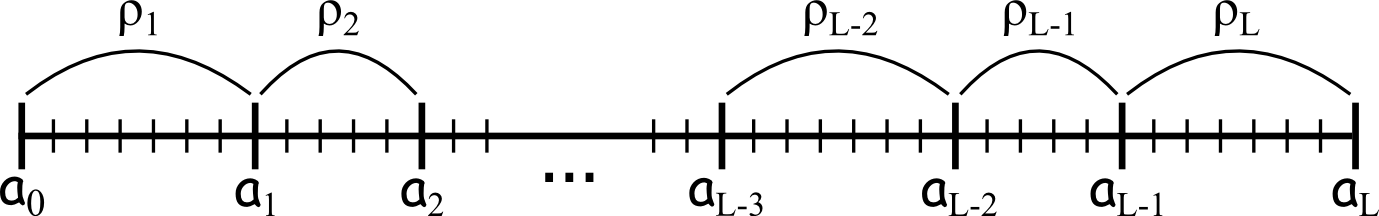
\includegraphics[width=15cm]{dinprog_default.png}
	\caption{Схема работы базового подхода динамического программирования}
	\label{fig:dinprog_default}
\end{figure}

Базовый подход работы данного алгоритма получается следующим.
Необходимо присвоить значения $a_{L-1}^j$, $j = \overline{-m, m}$ узлу $a_{L-1}$, в итоге, всего $2m+1$ значений.
Необходимо вычислить в части $[a_{L-1}^j + 1; a_L]$ оценку среднего коэффициента корреляции $\rho_L^j$ для всех $a_{L-1}^j$, что в сумме даст $2m + 1$ значений средних.
В данном случае, вследствие фиксации правой границы $a_L$, количество вариантов незначительно.
В итоге этого этапа фиксируются значения $a_{L-1}^j$ и соответствующие им оценки средних коэффициентов корреляции $\rho_L^j$, $j = \overline{-m, m}$.

Во время второго этапа изменениям подвергается граница $a_{L-2}$, расположенная слева, которой присваиваются значения $a_{L-2}^j$, $j = \overline{-m, m}$.
Но следует заметить, что в таком случае существует необходимость перебрать значения границы, расположенной справа $a_{L-1}^i$, $i = \overline{-m, m}$.
Для этого рассчитываются показатели оценок среднего коэффициента корреляции $\rho_{L-1}^{j, i}$, всего $(2m + 1)^2$ коэффициентов по количеству комбинаций для каждой конкретной комбинации $[a_{L-2}^j + 1; a_{L-1}^i]$.
В итоге каждому значению $a_{L-2}^j$ соответствует $2m + 1$ возможных положений границы $a_{L-1}^i$.
Из этих $2m + 1$ вариантов границ легко выбрать оптимальный в смысле максимума суммы оценок средних коэффициентов корреляции (далее для краткости суммарные оценки) в частях $[a_{L-2} + 1; a_{L-1}]$ и $[a_{L-1} + 1; a_L]$:
\begin{equation}
P_{L-1}^j = \max_{i} \{\rho_{L-1}^{j, i} + \rho_L^i \}.
\end{equation}

Итак, в результате второго этапа получены значения $a_{L-2}^j$ и соответствующие им суммарные оценки для двух крайних справа частей со значениями $P_{L-1}^j$.
Аналогично в результате третьего этапа получим для значений $a_{L-3}^j$ соответствующие им суммарные оценки для трёх крайних справа частей со значениями $P_{L-2}^j$, вычисляемыми по формуле
\begin{equation}
P_{L-2}^j = \max_{i} \{\rho_{L-2}^{j, i} + P_{L-1}^i \}.
\end{equation}

На предпоследнем этапе для узла $a_1$ получаем значения $a_1^j$ и выбираем оптимальный вариант, соответствующий максимальной суммарной оценке по всем частям:
\begin{equation}
P_1 = \max_{j} \{\rho_1^j + P_2^j \}.
\end{equation}

Рассмотренный алгоритм обеспечивает нахождение границ частей, оптимальных по критерию однородности $J_1$.
Для критерия $J_3$, также характеризующего однородность внутри части, задача решается аналогично. 

%\newpage
%============================================================================================================================

\subsection{Создание модифицированной схемы динамического программирования} \label{sect2_2_5}

Необходимость модификации стандартной модели обусловлена применением критерия, который зависит от обеих смежных частей с границами, заданными тремя узлами.
Предположим, что применяется составной критерий $J_{12}$, содержащий средние коэффициенты корреляции, как внутри одной части, так и между ними.
Рисунок \ref{fig:dinprog_modified} представляет границы частей и средние коэффициенты корреляции.

\begin{figure}[h]
	\centering
	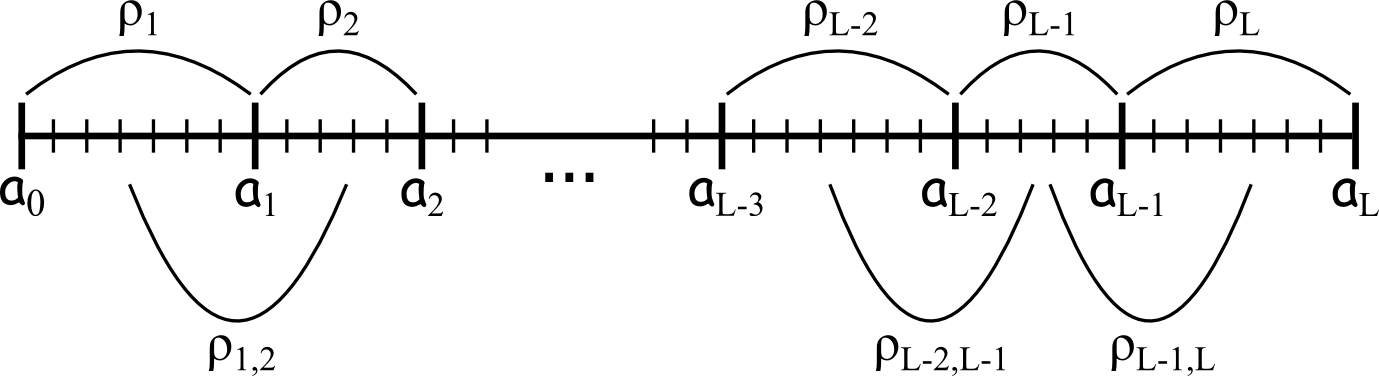
\includegraphics[width=15cm]{dinprog_modified.png}
	\caption{Схема работы предложенной модифицированной схемы динамического программирования}
	\label{fig:dinprog_modified}
\end{figure}

Здесь, в отличие от стандартной схемы, на каждом шаге следует перебирать значения не двух, а трёх узлов, то есть смотреть сразу на две части, что обусловлено взаимосвязью между смежными частями слов.

Был использован следующий доработанный алгоритм.
Во время первого этапа следует рассмотреть 2 крайние правые части.
Как и до этого, крайний узел $a_L$ принимается в качестве фиксированного.
Необходимо задать показатели приращения обеим другим узлам и перебрать все возможные сочетания положений границы $a_{L-1}^i$, $i = \overline{-m, m}$, $a_{L-2}^j$, $j = \overline{-m, m}$, что даёт $(2m + 1)^2$ комбинаций.
Оба изучаемых узла в полной мере задают значения двух крайних частей, находящихся справа, благодаря чему возможно рассчитать значение критерия $J_{12}$ для любого варианта их расположения.

Для проведения данной операции необходимо найти значение внутри всех частей $\rho_L^i$, $\rho_{L-1}^{j, i}$ и между частями $\rho_{L-1, L}^{j, i}$ средних коэффициентов корреляции для каждой пары индексов $i$ и $j$.
После чего для обеих частей $[a_{L-1} + 1; a_L]$ и $[a_{L-2} + 1; a_{L-1}]$ по формуле рассчитать средние коэффициенты корреляции (суммарные оценки):
\begin{equation}
P_{L-1, L}^{j, i} = \rho_L^i + \rho_{L-1}^{j, i} + \rho_{L-1, L}^{j, i}.
\end{equation}

Всего получаем $(2m + 1)^2$ значений суммарных оценок, которые приписываем каждой из $(2m + 1)^2$ комбинаций значений узлов $a_{L-1}^i$ и $a_{L-2}^j$.
В этом заключается результат первого этапа.
Во время второго этапа необходимо ввести узел $a_{L-3}$ и придать ему $2m + 1$ значений $a_{L-3}^l$, $l = \overline{-m, m}$.
Новый узел позволяет вычислить коэффициенты $\rho_{L-2}$ и $\rho_{L-2, L-1}$.
Эти коэффициенты, зависят также от значений границ предыдущей части, то есть от значений $a_{L-2}^j$ и $a_{L-1}^i$.
Используя эти значения и перебирая $(2m + 1)^3$ комбинаций по переменным $l$, $j$, $i$ вычисляем суммарные оценки
\begin{equation}
P_{L-2, L-1}^{l, j, i} = \rho_{L-2}^{l, j} + \rho_{L-2, L-1}^{l, j, i} + P_{L-1, L}^{j, i}.
\end{equation}

Итоговые количество рассчитанных значений равно $(2m + 1)^3$.
Выделим значения, соответствующие узлам $a_{L-3}$ и $a_{L-2}$, то есть индексам $l$, $j$.
У любой из комбинаций этих коэффициентов есть соответствующие $2m + 1$ значения узла $a_{L-1}$, или, что то же самое, индекса $i$.
Возьмём по индексу $i$ максимум.
В итоге получим $(2m + 1)^2$ значений суммарного коэффициента, соответствующую узлам $a_{L-3}$ и $a_{L-2}$:
\begin{equation}
P_{L-2, L-1}^{l, j} = \max_{i} \{ P_{L-2, L-1}^{l, j, i} \}.
\end{equation}

В результате второй этапа получим $(2m + 1)^2$ сочетаний коэффициентов $a_{L-3}$ и $a_{L-2}$.
При этом каждому из них будет приписана оптимальная по всем вероятным значениям узла $a_{L-1}$ величина совокупной оценки.
Соответственно, на предпоследнем этапе для узлов $a_1$ и $a_2$ количество значений составит $(2m + 1)^2$, которым по отдельности будет приписана оптимальная по всем доступным позициям узлов $a_3, \dots, a_{L-1}$ величина общей оценки:
\begin{equation}
P_{1, 2}^{k, j} = \max_{i} \{ P_{1, 2}^{k, j, i} \}.
\end{equation}

На последнем этапе добавляем узел $a_0$ и находим оптимальный вариант:
\begin{equation}
P_{1, 2} = \max_{l, j} \{ \rho_1^l + \rho_{1, 2}^{l, j} + P_{1, 2}^{l, j} \}.
\end{equation}

Таким образом, предложенная модифицированная схема метода динамического программирования является более сложной и требует перебора $(2m + 1)^3$ комбинаций вместо $(2m + 1)^2$ в стандартной схеме.
Обусловлено это тем, что вариант с модификациями соответствует критерию с введёнными составляющими, зависящими сразу от обеих смежных частей.
Ввиду этого необходимо углубить параметры перебора.

Результаты работы приведённых алгоритмов динамического программирования показаны в подразделе \ref{sect3_2}.

%\newpage
%============================================================================================================================

\section{Разработка алгоритма формирования эталонов на основе метода главных компонент} \label{sect2_3}

Представляется алгоритм оптимизации эталона, осуществляющий уменьшение размерности задачи оптимизации, посредством использования метода главных компонент.
Теоретическое описание метода главных компонент приведено в подразделе \ref{sect1_4_3}.

Формирование оптимального эталона заключается в разделении на главные компоненты и в последующей оптимизации коэффициентов разделения с помощью метода покоординатного спуска на обучающей выборке.
В представленном подразделе приведён алгоритм для получения оптимального эталона и описание способа расчёта главных компонент для рассматриваемой задачи.
Полученный в результате оптимизации эталон может быть применён в любых алгоритмах, которые используют сравнение с эталоном.
С целью снижения времени работы алгоритма рассматривается и метод его упрощения, при сохранении качества результатов.
Результаты тестирования, подтверждающие работоспособность предложенного подхода на примерах распознавания слов естественного русского языка с помощью новых эталонов представлены в подразделе \ref{sect3_3}.

%\newpage
%============================================================================================================================

\subsection{Описание алгоритма разложения спектрального портрета слова на главные компоненты} \label{sect2_3_1}

Пусть имеется $M$ параметрических портретов различных реализаций одного слова $X = \{x_{ij}(k)\}$, $k = 1, 2, \dots, M$; $i = 1, 2, \dots, N_t$; $j = 1, 2, \dots, N_f$.
Процедура формирования параметрических портретов слов подробно описана в подразделе \ref{sect1_2_1}.
Необходимо преобразовать матричный портрет для всех $k$ в одномерный массив с количеством элементов $l = 1, 2, \dots, P$, $P = N_f N_t$.
Итак, имеем $M$ векторов размерности $P$ каждый: $\{x_{lk}\}$, $k = 1, 2, \dots, M$; $l = 1, 2, \dots, P$.
В явном виде:

\begin{equation} \label{eq:2_3_1_1}
x_1 = \begin{bmatrix} x_{11} \\ x_{21} \\ \vdots \\ x_{P1} \end{bmatrix} \text{,  }
x_2 = \begin{bmatrix} x_{12} \\ x_{22} \\ \vdots \\ x_{P2} \end{bmatrix} \text{,  }
\dots
x_M = \begin{bmatrix} x_{1M} \\ x_{2M} \\ \vdots \\ x_{PM} \end{bmatrix} \text{,  }
\end{equation}

Объединим эти $M$ векторов в матрицу размерности $P \times M$:

\begin{equation} \label{eq:2_3_1_2}
X = \begin{bmatrix} x_1 & x_2 & \dots & x_M \end{bmatrix} = 
\begin{bmatrix}
x_{11} & x_{12} & \dots  & x_{1M} \\
x_{21} & x_{22} & \dots  & x_{2M} \\ 
\vdots & \vdots & \ddots & \vdots \\
x_{P1} & x_{P2} & \dots  & x_{PM} \\
\end{bmatrix}.
\end{equation}

Далее необходимо провести вычисление матрицы корреляционных моментов векторов $x_1, x_2, \dots, x_M$, имеющих размерность $M \times M$:

\begin{equation} \label{eq:2_3_1_3}
K_x = X^T X =
\begin{bmatrix} x_1^T \\ x_2^T \\ \vdots \\ x_M^T \end{bmatrix} \begin{bmatrix} x_1 & x_2 & \dots & x_M \end{bmatrix} = 
\begin{bmatrix}
x_1^T x_1 & x_1^T x_2 & \dots  & x_1^T x_M \\
x_2^T x_1 & x_2^T x_2 & \dots  & x_2^T x_M \\
\vdots    & \vdots    & \ddots & \vdots    \\
x_M^T x_1 & x_M^T x_2 & \dots  & x_M^T x_M \\
\end{bmatrix}.
\end{equation}

Заметим, что в матрице $K_x$ каждый элемент есть скалярное произведение соответствующих векторов и матрица $K_x$ симметричная.
Для неё можно вычислить $M$ собственных чисел $\lambda_1, \lambda_2, \dots, \lambda_M$ и соответствующих собственных векторов $l_1, l_2, \dots, l_M$ размерности $M$.
Собственные числа можно упорядочить по убыванию $\lambda_1 \ge \lambda_2 \ge \dots \ge \lambda_M$.

Определить первую главную компоненту $a_1$ необходимо как линейную комбинацию базовых векторов $x_1, x_2, \dots, x_M$, коэффициенты которых должны быть равны элементам их собственного вектора $l_1^T= [l_{11} l_{21} \dots l_{M1}]$:

\begin{equation} \label{eq:2_3_1_4}
a_1 = l_{11} x_1 + l_{21} x_2 + \dots + l_{M1} x_M = \sum_{i=1}^M l_{i1} x_i.
\end{equation}

Для главных компонент $m = 2, 3, \dots, M$ проводятся аналогичные расчёты по формуле:

\begin{equation} \label{eq:2_3_1_5}
a_k = \sum_{k=1}^M l_{km} x_k.
\end{equation}

В соответствии с теоретическими выкладками, представленными в подразделе \ref{sect1_2_2} сумма дисперсий исходных векторов и сумма дисперсий главных компонентов равны.
Таким образом, энергия сигналов при преобразование не изменяется.
Значение дисперсии главной компоненты $a_j$ равняется собственному числу $\lambda_j$.
Взаимная ортогональность является важным свойством главных компонент.
Целесообразность использования главных компонент заключается в наиболее существенном влиянии первых главных компонент на поведение системы $a_j$, $j = 1, 2, \dots, M'$.
Что делает возможным снизить размерность задачи и использовать $M'$ главных компонент вместо $M$ исходных векторов.
При необходимости оценить погрешность, связанную с переходом от $M$ изначальных векторов к $M'$ главным компонентам, можно воспользоваться величиной

\begin{equation} \label{eq:2_3_1_6}
I_p = \frac{\lambda_1 + \lambda_2 + \dots + \lambda_{M'}}{\lambda_1 + \lambda_2 + \dots + \lambda_M}.
\end{equation}

Как правило, первые несколько компонент содержат почти всю информацию о параметрическом портрете.
В подразделе \ref{sect3_3_1} будет определено количество главных компонент, которые несут существенную информацию о параметрическом портрете.
Также там будут приведены другие статистические расчёты, показывающие правильность работы метода главных компонент.

%\newpage
%============================================================================================================================

\subsection{Описание алгоритма формирования оптимизированных эталонов на основе метода главных компонент} \label{sect2_3_2}

Пусть эталоны для каждого из распознаваемых слов в словаре сформированы как усреднённый параметрический портрет всех реализаций.
Количественная оценка ошибок распознавания на выбранном диапазоне дикторов является наиболее простым способом оценки качества полученных эталонов.
Но при малом числе ошибок такая дискретная мера оценки качества распознавания не будет информативной и эффективной.
Поэтому целесообразно перейти к использованию некой непрерывной меры оценки качества распознавания.
Нижняя граница числового значения Z-преобразования Фишера коэффициента корреляции эталона с исследуемым словом может быть рассмотрена в виде такой непрерывной меры.
Просуммировав эти значения для каждого эталона, получим максимизируемую целевую функцию.

Другими словами, мера оценки качества распознавания трёх слов описывается следующей формулой:

\begin{equation} \label{eq:2_3_2_1}
F = \Delta Z^{low}_{1} + \Delta Z^{low}_{2} + \Delta Z^{low}_{3},
\end{equation}
где $\Delta Z^{low}_{i}$ определяется следующим образом:
\begin{equation} \label{eq:2_3_2_2}
\Delta Z^{low}_{i} = \min(\Delta Z_{ij}, \Delta Z_{ik}), \qquad i \ne j, i \ne k, j \ne k,
\end{equation}
а $\Delta Z_{ij}$ --- это разница Z-преобразований Фишера коэффициентов корреляций эталона $i$-го с распознаваемым $i$-м словом и эталона $j$-го с распознаваемым $i$-м словом.

Также можно дополнительно штрафовать за неправильное распознавание слова, что эквивалентно штрафу за значения $Z^{low}_{i}$ меньше нуля:

\begin{equation} \label{eq:2_3_2_3}
F = \Delta Z^{*low}_{1} + \Delta Z^{*low}_{2} + \Delta Z^{*low}_{3} \text{, где }
\Delta Z^{*low}_{i} = \left\{
\begin{array}{ll}
\Delta Z^{low}_{i}, \qquad\qquad\qquad \Delta Z^{low}_{i} \ge 0,\\
\Delta Z^{low}_{i} - \alpha (\Delta Z^{low}_{i})^2, \Delta Z^{low}_{i} < 0,
\end{array}
\right.
\end{equation}
где $\alpha$ --- это некоторое положительное число.

В формуле \eqref{eq:2_3_2_3} вместо нуля можно использовать любое другое положительно значение, которое будет интерпретироваться как зазор для устойчивости правильного распознавания.

Далее рассмотрим параметрический портрет эталона в виде линейной комбинации константы и $M'$ главных компонент с некоторыми коэффициентами: 

\begin{equation} \label{eq:2_3_2_4}
E_{syn} = k_0 a_0 + k_1 a_1 + \dots + k_{M'} a_{M'}.
\end{equation}

Задача получения оптимального эталона сводится к нахождению коэффициентов $k_0, \dots, k_{M'}$ таких, для которых должен выполняться критерий: $N_{ошибок} \rightarrow \min$, или величина Z коэффициента корреляции $\rightarrow \max$.
Подбор коэффициентов $k_0, \dots, k_{M'}$ можно произвести используя численные методы.

При построении $M'$ главных компонент может используется речевой материал нескольких дикторов.
Изначальное приближение коэффициентов рекомендуется выбирать из средних значений коэффициентов усреднённого эталона (выбранное как среднее из взятых эталонов) по результатам $M'$ главных компонент.
Дальнейшая оптимизация коэффициентов производится на обучающем наборе данных, который в общем случае может не совпадать с речевым материалом, по которому был получен эталон и начальное приближение коэффициентов.

В качестве метода оптимизации $F = f(k_0, \dots, k_{M'})$ выберем метод покоординатного спуска \cite{alekseeva2008, luenberger1984linear}.
Закон изменения коэффициентов разложения при $k_j > 0.001$: $k_{j+1} = k_j + l \Delta k_j$, $\Delta k_j = 0.01 |k_j|$, $l = 0, \pm 1, \pm 2, \pm 3, \pm 5, \pm 10, \pm 15, \pm 25, \pm 50, \pm 100, \pm 200$.
При условии $k_j \le 0.001$ применяется закон изменения с неизменным шагом: $k_{j+1} = k_j + 0.001 \Delta k_j$, $\Delta k_j = 0, \pm 1, \pm 2, \pm 3, \dots, \pm 10$.

Критерий остановки:
\begin{equation} \label{eq:2_3_2_5}
|F_{i+1} - F_i| \le \epsilon,\qquad \epsilon = 0.02 |F_i|.
\end{equation}

Другими словами, оптимизация завершается, когда значение оптимизируемой целевой функции изменяется меньше чем на 2~\%.
Независимый подбор коэффициентов для каждого слова является простым способом подбора, при котором коэффициенты разложения другой пары слов не меняются и остаются равными изначальному приближению.
В этом случае можно в качестве целевой функции использовать отдельные слагаемые из формул \eqref{eq:2_3_2_1} и \eqref{eq:2_3_2_3}.
Более сложный вариант заключается в оптимизации коэффициентов для каждого слова на каждой итерации оптимизационного процесса.
Тогда нужно использовать полную версию оптимизируемой целевой функции $F$.

В подразделах \ref{sect3_3_2} и \ref{sect3_3_3} будут приведены результаты оптимизации эталона с помощью предложенного метода, а также результаты распознавания слов оптимизированным эталоном.

%\newpage
%============================================================================================================================

\section{Разработка алгоритма формирования эталонов на основе полиномов Чебышёва} \label{sect2_4}

В данном подразделе рассматривается разработка алгоритма формирования эталонов на основе полиномов Чебышёва.
Теоретическое описание разложения произвольной функции на базис, образованный многочленами Чебышёва, дано в подразделе \ref{sect1_4_5}.

Пусть у нас есть параметрический портрет $X$, который содержит $N_f$ частотных полос и $N_t$ временных интервалов.
Данный параметрический портрет помимо самого речевого сигнала содержит ещё и неинформативные сигналы, обусловленные особенностями речи определённого диктора и шумами.
Использование полиномов Чебышёва поможет выделить только информативную часть, решив при этом сразу несколько задач.
Во-первых, это позволит уменьшить размерность параметрического портрета без существенной потери информативности, что упростит его хранение и ускорит обработку.
Вычислительная эффективность является одним из приоритетов разрабатываемых алгоритмов, поэтому ускорение обработки портретов является несомненным плюсом.

Во-вторых, выделение только самого речевого сигнала может помочь повысить качество распознавания.
При этом, можно проводить распознавание как сжатой версии параметрического портрета, так и восстановленной версии, которая не будет содержать лишних шумов.

Сжатие можно производить по частотным полосам, по временным интервалам и по обоим измерениям одновременно.
Для последнего случая получится сжатый параметрический портрет с $N'_f < N_f$ частотными полосами и $N'_t < N_t$ временными интервалами.
Суммарное количество элементов параметрического портрета уменьшится с $N_f \cdot N_t$ до $N'_f \cdot N'_t$.
Также возможно использование сжатие параметрических портретов с использованием полиномов Чебышёва не только для записей слов, но и для эталонов.

Результаты проверки сжатия параметрических портретов описаны в подразделе \ref{sect3_4}.

%\newpage
%============================================================================================================================

\section{Разработка алгоритмов формирования эталонов по нескольким дикторам на основе формулы Байеса и метода комитетов} \label{sect2_5}

Рассмотрена задача распознавания слов с использованием нескольких эталонов.
Общеизвестным фактом является то, что индивидуальные особенности диктора обуславливают параметры речи \cite{rabiner1993fundamentals, korsun2017recognition}.
Необходимо больше разнообразить речевой материал обучающей базы, с целью исключить дикторозависимость автоматического распознавания.
К примеру, можно использовать большее количество эталонов, при формировании которых применялись записи различных дикторов.

В данном подразделе предлагаются два алгоритма распознавания речевых команд с использованием нескольких эталонов. 
Первый алгоритм использует формулу Байеса \cite{ventcel1999theory}.
При данной методологии априорные условные вероятности гипотетических вариантов распознавания слов формируются на базе обучающей выборки, а затем найденные вероятности применяются при расчётах апостериорных вероятностей уже по факту получения результатов распознавания.
Благодаря этому удаётся повысить качество оценки, что, в свою очередь, положительно влияет на качество распознавания в условиях, когда невозможно произвести выбор состава команд.

В основе второго алгоритма лежит метод комитетов, в основе которого лежит независимое распознавание команд с помощью различных эталонов.
Данный алгоритм является модификацией стандартного метода комитетов, описанного в подразделе \ref{sect1_4_6}.
Всем возможным вариантам распознавания присваивается определённый балл.
В дальнейшем необходимо получить сумму полученных по всем эталонам баллов для формирования заключительной оценки, лежащей в основе определения результата распознавания.

Теоретическое обоснование представленных алгоритмов приведено ниже.
В данных алгоритмах для улучшения результатов распознавания могут быть применены подстройка по времени, описанная в подразделе \ref{sect2_2}, и оптимизированные эталоны, описанные в подразделе \ref{sect2_3}.
Также для ускорения работы алгоритмов может быть использовано сжатие используемых параметрических портретов, описанное в подразделе \ref{sect2_4}.
Для каждого из приведённых алгоритмов в подразделе \ref{sect3_5} представлены результаты экспериментальных исследований, подтверждающие их работоспособность.

%\newpage
%============================================================================================================================

\subsection{Алгоритм на основе формулы Байеса: определение задачи} \label{sect2_5_1}

В этом разделе также описывает решение задачи распознавания изолированных друг от друга команд.
Допустим, что в наличие есть гипотезы $H_1, H_2, \dots, H_M$ априорные вероятности которых составляют $P(H_1), P(H_2), \dots, P(H_M)$.
При распознавании им должны соответствовать $M$ различных слов.
В случае, когда по итогам распознавания принимается гипотеза $H_n$, можно сказать, что имело место событие $A_n$.
Предположим, что с целью распознавания получены $L$ разных эталонов, каждый состоящий из $M$ субэталонов, соответствующих отдельным словам.
Все субэталоны характеризует собой обобщённый параметрический портрет только одного слова из $M$ слов \cite{rabiner1993fundamentals, korsun2017recognition, korsun2016automatic}.
В основном, особенности всех $L$ эталонов обусловлены тем, что они составляются на базе речевого материала разных дикторов, ввиду чего и учитывают индивидуальные особенности его речи.
Тем не менее, вероятны и другие причины.

Распознавание по любому из $L$ эталонов производится путём последовательного вычисления скалярной меры близости $Z$ между параметрическим портретом распознаваемого слова и каждым из $M$ субэталонов.
Верной считается гипотеза, которая соответствует эталону слова с мерой близости $Z$, имеющей экстремум.
Традиционный порядок распознавания по единственному эталону соответствует этому \cite{rabiner1993fundamentals}.
В качестве меры близости может выбираться евклидово расстояние или расстояние Махаланобиса между векторами параметрического портрета \cite{rabiner1993fundamentals}, коэффициент корреляции \cite{korsun2016automatic}, Z-преобразование Фишера от коэффициента корреляции \cite{korsun2017recognition} и так далее.
Необходимо сформулировать задачу создания более качественной с математической точки зрения процедуры сравнения, позволяющей получить вероятностные оценки каждой гипотезы.
В первую очередь, это сделает возможным формирование иерархии наиболее вероятных гипотез даже после проведения процедуры распознавания с одним эталоном.
Кроме того, при использовании всех $L$ эталонов это позволит создать математически верный алгоритм для распознавания.
За основу возьмём формулу Байеса, используемую для вычисления апостериорных вероятностей \cite{ventcel1999theory}.
В первую очередь необходимо описать процедуру распознавания с использованием одного эталона.

Давайте предположим, что есть гипотезы $H_1, H_2, \dots, H_M$, которые соответствуют полной группе несовместных событий, характеризующихся значениями априорных вероятностей $P(H_1), P(H_2), \dots, P(H_M)$.
Пусть в результате распознавания по одному эталону произошло событие $A_k$, то есть принята гипотеза $H_k$.
В таком случае условная апостериорная вероятность любой из гипотез по формуле Байеса \cite{ventcel1999theory}, при выполнении условия наступления событий $A_{k_1}$, равняется:

\begin{equation}\label{eq:2_5_1_1}
P(H_i|A_k) = \frac{P(H_i) P(A_k|H_i)}{P(A_k)},
\qquad
i = 1, 2, \dots, M,
\end{equation}
\begin{itemize}[align=left,leftmargin=1.8em,itemindent=0pt,labelsep=0pt,labelwidth=1.8em]
	\item[где] $P(A_k|H_i)$ --- условная априорная вероятность события $A_k$ при условии, что верна гипотеза $H_i$.
\end{itemize}

Отметим, что событие $A_k$ может произойти только вместе с одним из событий $H_1, H_2, \dots, H_M$.
Тогда по формуле полной вероятности \cite{ventcel1999theory} вероятность события $A_k$ $P(A_k) = \sum_{j=1}^M P(H_j) P(A_k|H_j)$.

Подставляя в \eqref{eq:2_5_1_1}, получим другой вариант формулы Байеса, который и будем использовать в дальнейшем:

\begin{equation}\label{eq:2_5_1_2}
P(H_i|A_k) = \frac{P(H_i) P(A_k|H_i)}{\sum_{j=1}^M P(H_j) P(A_k|H_j)},
\qquad
i = 1, 2, \dots, M.
\end{equation}

Найти апостериорные вероятности любой гипотезы в условиях распознавания лишь по одному эталону можно по формуле \eqref{eq:2_5_1_2}.
Чтобы её было возможно применить, следует прежде оценить априорные вероятности гипотез $P(H_1), P(H_2), \dots, P(H_M)$, $i = 1, 2, \dots, M$, и найти для каждого события $A_k$ оценки априорных вероятностей событий $P(A_k|H_i)$, $k = 1, 2, \dots, M$, $i = 1, 2, \dots, M$.
Также требуется разработать алгоритм для подсчёта апостериорных вероятностей гипотез $H_i$ в условиях наличия производного количества эталонов.
Эти вопросы рассматриваются далее.

%\newpage
%============================================================================================================================

\subsection{Оценка априорных вероятностей экспериментальным методом} \label{sect2_5_2}

Формула Байеса \eqref{eq:2_5_1_2} включает априорные вероятности $P(H_i)$, $i = 1, 2, \dots, M$ каждой гипотезы.
Допускается давать им оценку равной вероятности, то есть $P(H_i) = 1/M$, а при многоэтапной процедуре распознавания --- исходить из апостериорной вероятности, основываясь на результатах предыдущего этапа.

Для применения формулы \eqref{eq:2_5_1_2} необходимо также получить оценки априорных условных вероятностей $P(A_k|H_i)$, $i = 1, 2, \dots, M$, то есть вероятностей события $A_k$ (вероятность признания гипотезы $H_k$ правильной) при условии, что верна гипотеза $H_i$, $i = 1, 2, \dots, M$.
С этой целью следует применить обучающую выборку.
Допустим, что обучающая выборка включает в себя $M$ слов по $E$ записей каждого.
В таком случае по итогам распознавания подсчитывается число событий $A_k$, $k = 1, 2, \dots, M$ для каждой гипотезы $H_i$, $i = 1, 2, \dots, M$.
Для нахождения оценки условных вероятностей можно использовать формулу:

\begin{equation}\label{eq:2_5_2_1}
P(A_k|H_i) = \frac{e_{ki}}{E},
\qquad
k = 1, 2, \dots, M,
\qquad
i = 1, 2, \dots, M,
\end{equation}
\begin{itemize}[align=left,leftmargin=1.8em,itemindent=0pt,labelsep=0pt,labelwidth=1.8em]
	\item[где] $e_{ki}$ --- число событий $A_k$ (верной признана гипотеза $H_k$), при условии, что верна гипотеза $H_i$.
\end{itemize}

Далее для расчёта апостериорных условных вероятностей $P(H_i|A_k)$ оценки, вычисленные по формуле \eqref{eq:2_5_2_1}, подставляются в \eqref{eq:2_5_1_2}.

%\newpage
%============================================================================================================================

\subsection{Методология расчёта апостериорных вероятностей гипотез в условиях применения более двух эталонов} \label{sect2_5_3}

Допустим, что исходно даны два эталона, используемых независимо друг от друга при распознавании.
В таком случае допускается использование формулы Байеса с целью определения показателей апостериорных вероятностей гипотез.
При двух эталонах следует рассматривать события $A_{k_1 k_2}$, соответствующие совместному распознаванию гипотез $H_{k_1}$ и $H_{k_2}$ по эталонам $C_1$ и $C_2$:

\begin{equation}\label{eq:2_5_3_1}
A_{k_1 k_2} = A_{k_1}^{C_1} A_{k_2}^{C_2},
\qquad
k_1 = 1, 2, \dots, M,
\qquad
k_2 = 1, 2, \dots, M,
\end{equation}
\begin{itemize}[align=left,leftmargin=1.8em,itemindent=0pt,labelsep=0pt,labelwidth=1.8em]
	\item[где] событие $A_{k_1}^{C_1}$ означает, что при распознавании по эталону $C_1$ верной признана гипотеза $H_{k_1}$,
	\item[] событие $A_{k_2}^{C_2}$ определено аналогично.
\end{itemize}

Событие $A_{kk}$ совпадения результатов распознавания по обоим эталоном является частным случаем \eqref{eq:2_5_3_1}.

\begin{equation}\label{eq:2_5_3_2}
A_{kk} = A_k^{C_1} A_k^{C_2}.
\end{equation}

Само собой, \eqref{eq:2_5_3_2} может быть выполнено в условиях корректного распознавания обоих эталонов, либо при совпадении их ошибок.

Условные вероятности события $A_{k_1 k_2}$ по гипотезам $H_i$ с учётом допущения о независимости распознаваний по эталонам 1 и 2

\begin{equation}\label{eq:2_5_3_3}
P(A_{k_1 k_2}|H_i) = P(A_{k_1}^{C_1}|H_i) P(A_{k_2}^{C_2}|H_i).
\end{equation}

При совпадении $k_1 = k_2 = k$ формула \eqref{eq:2_5_3_3} принимает вид

\begin{equation}\label{eq:2_5_3_4}
P(A_{kk}|H_i) = P(A_{k}^{C_1}|H_i) P(A_{k}^{C_2}|H_i).
\end{equation}

Условные вероятности событий $A_{k_1}^{C_1}$ и $A_{k_2}^{C_2}$ по гипотезам $H_i$ находятся отдельно для каждого эталона по обучающей выборке в соответствии с формулой \eqref{eq:2_5_2_1} предыдущего подраздела.

При двух эталонах формула Байеса \eqref{eq:2_5_1_2} принимает вид:

\begin{equation}\label{eq:2_5_3_5}
P(H_i|A_{k_1 k_2}) = \frac{P(H_i) P(A_{k_1 k_2}|H_i)}{\sum_{j=1}^M P(H_j) P(A_{k_1 k_2}|H_j)}.
\end{equation}

Для произвольного числа $L$ применяемых независимо эталонов рассмотрим событие

\begin{equation}\label{eq:2_5_3_6}
A_{k_1 k_2 \dots k_L} = A_{k_1}^{C_1} A_{k_2}^{C_2} \dots A_{k_L}^{C_L}
\end{equation}
и его частный случай

\begin{equation}\label{eq:2_5_3_7}
A_{kk \dots k} = A_{k}^{C_1} A_{k}^{C_2} \dots A_{k}^{C_L}.
\end{equation}

Формула \eqref{eq:2_5_3_4} для условных вероятностей события $A_{k_1 k_2 \dots k_L}$ при допущении о независимости эталонов принимает вид:

\begin{equation}\label{eq:2_5_3_8}
P(A_{k_1 k_2 \dots k_L}|H_i) = P(A_{k_1}^{C_1}|H_i) P(A_{k_2}^{C_2}|H_i) \dots P(A_{k_L}^{C_L}|H_i) = \prod_{j=1}^{L} P(A_{k_j}^{C_j}|H_i).
\end{equation}

В случае совпадения результатов всех $L$ эталонов $k_1 = k_2 = \dots = k_L = k$:

\begin{equation}\label{eq:2_5_3_9}
P(A_{k}|H_i) = \prod_{j=1}^{L} P(A_{k}^{C_j}|H_i).
\end{equation}

Для случая $L$ эталонов в формуле Байеса \eqref{eq:2_5_3_5} необходимо изменить только количество индексов:

\begin{equation}\label{eq:2_5_3_10}
P(H_i|A_{k_1 k_2 \dots k_L}) = \frac{P(H_i) P(A_{k_1 k_2 \dots k_L}|H_i)}{\sum_{j=1}^M P(H_j) P(A_{k_1 k_2 \dots k_L}|H_j)}.
\end{equation}

Таким образом, полученный на основе формулы Байеса алгоритм позволяет находить апостериорные вероятности каждой гипотезы по результатам распознавания с произвольным числом эталонов.
Естественно, что именно гипотеза с наибольшей апостериорной вероятностью признается результатом распознавания.

%\newpage
%============================================================================================================================

\subsection{Введение учёта качества распознавания} \label{sect2_5_4}

В подразделах, представленных ранее, применялся исключительно итоговый результат при проведении процедуры распознавания по каждому эталону.
Таким образом, бралась только та гипотеза, которая соответствовала значению экстремума меры близости субэталона и распознаваемого слова.
Ещё одной возможностью повышения качества распознавания является применение значений меры близости $Z$ для оценки его качества.
Вначале рассмотрим распознавание по одному эталону.

Предположим для определённости, что наибольшее сходство соответствует максимуму меры близости $Z$.
Введём показатель $\Delta Z = Z_{\max} - Z_{\max - 1}$, где $Z_{\max}$ --- максимальное значением меры близости $Z_{\max}$ между параметрическими портретами распознаваемого слова и всеми $M$ субэталонами, а $Z_{\max - 1}$ --- значение, ближайшее к максимальному.
Значение $\Delta Z$ можно использовать для оценки качества распознавания.
Действительно, доверять результатам распознавания можно тем больше, чем сильнее выделяется наилучшее слово (лучший субэталон) в сравнении с другими словами.
Ввиду этого можно допустить, что показатели качества распознавания зависят и прямо пропорциональны количественным значениям величины $\Delta Z$.

Выше мы рассматривали событие $A_k$ (гипотеза $H_k$ признается верной) условием которого является верность гипотезы $H_i$.
Соответствующая условная вероятность $P(A_{k}|H_i)$ определялась по обучающей выборке.
Теперь рассмотрим событие $A_k^{\Delta Z}$, заключающееся в совместном появлении события $A_k$ и значения показателя качества $\Delta Z$ при том же условии --- верна гипотеза $H_i$.
Принимая допущение о независимости, получим для условной вероятности события $A_k^{\Delta Z}$ по гипотезе $H_i$:

\begin{equation}\label{eq:2_5_4_1}
P(A_k^{\Delta Z}|H_i) = P(A_k|H_i) P(\Delta Z|H_i),
\quad
k = 1, 2, \dots, M,
\quad
i = 1, 2, \dots, M.
\end{equation}

Нахождение оценок вероятности $P(A_k|H_i)$ описано в предыдущих подразделах.
Для получения оценок вероятности $P(\Delta Z|H_i)$ появления наблюдаемого значения $\Delta Z$ в случае, если верна гипотеза $H_i$, предложим следующий алгоритм.

Пусть на обучающей выборке выполнено распознавание, как и ранее.
Теперь дополнительно вычислим и зафиксируем показатели $\Delta Z$ для каждого распознаваемого слова.
Разобьём диапазон значений показателя $\Delta Z$ на $N_{\Delta Z} = 6 \dots 8$ полос, которым присвоим обозначения $\Delta Z_j, j = 1, \dots, N_{\Delta Z}$.
Примем во внимание, что, если верна гипотеза $H_i$, возможны как правильные, так и неправильные распознавания. Тогда для каждой полосы $\Delta Z_j, j = 1, \dots, N_{\Delta Z}$ оценки условных вероятностей появления значения $\Delta Z \in \Delta Z_j$ определяются по формулам:

\begin{equation}\label{eq:2_5_4_2}
P_c(\Delta Z_j|H_i) = \frac{n_c^i(\Delta Z_j)}{n_c^i(\Delta Z_j) + n_{nc}^i(\Delta Z_j)},
\qquad
i = 1, 2, \dots, M,
\end{equation}

\begin{equation}\label{eq:2_5_4_3}
P_{nc}(\Delta Z_j|H_i) = \frac{n_{nc}^i(\Delta Z_j)}{n_c^i(\Delta Z_j) + n_{nc}^i(\Delta Z_j)},
\qquad
j = 1, 2, \dots, N_{\Delta Z},
\end{equation}
\begin{itemize}[align=left,leftmargin=1.8em,itemindent=0pt,labelsep=0pt,labelwidth=1.8em]
	\item[где] $P_c(\Delta Z_j|H_i)$ --- оценка условной вероятности появления значения $\Delta Z \in \Delta Z_j$ при правильном распознавании, если верна гипотеза $H_i$;
	\item[] $P_{nc}(\Delta Z_j|H_i)$ --- оценка условной вероятности появления значения $\Delta Z \in \Delta Z_j$ при неправильном распознавании, если верна гипотеза $H_i$;
	\item[] $n_c^i(\Delta Z_j)$, $n_{nc}^i(\Delta Z_j)$ --- количество соответственно правильных и неправильных распознаваний, если показатель $\Delta Z$ принадлежит полосе $\Delta Z_j$ при условии, что верна гипотеза $H_i$.
\end{itemize}

Объединяя вероятности \eqref{eq:2_5_4_2} и \eqref{eq:2_5_4_3} по всем $j = 1, 2, \dots, N_{\Delta Z}$ полосам, получим условные вероятности появления значения $\Delta Z$ по всем гипотезам $H_i$, то есть если верна гипотеза $H_i$, $i = 1, 2, \dots, M$.
Присвоим этим условным вероятностям выражения $P_c(\Delta Z_j|H_i)$ и $P_{nc}(\Delta Z_j|H_i)$.
Тогда условная вероятность $P(\Delta Z|H_i)$, необходимая для расчёта условной вероятности события $A_k^{\Delta Z}$ по формуле \eqref{eq:2_5_4_1}, определяется следующим образом:

\begin{equation}\label{eq:2_5_4_4}
P(\Delta Z|H_i) = P_c(\Delta Z|H_i), \text{ если } i=k, \text{ и } P(\Delta Z|H_i) = P_{nc}(\Delta Z|H_i), \text{ если } i \ne k.
\end{equation}

Если в формулу Байеса \eqref{eq:2_5_1_2} подставить \eqref{eq:2_5_4_4}, будет получена формула для расчёта значений апостериорных вероятностей, учитывающих показатель качества распознавания $\Delta Z$:

\begin{equation}\label{eq:2_5_4_5}
P(H_i|A_k^{\Delta Z}) = \frac{P(H_i) P(A_k^{\Delta Z}|H_i)}{\sum_{j=1}^M P(H_j) P(A_k^{\Delta Z}|H_j)}
= \frac{P(H_i) P(A_k|H_i) P(\Delta Z|H_i)}{\sum_{j=1}^M P(H_j) P(A_k|H_j) P(\Delta Z|H_j)}.
\end{equation}

Рассчитать оценки вероятности $P^{C_1}(\Delta Z^1|H_i)$ и $P^{C_2}(\Delta Z^2|H_i)$ для каждого эталона отдельно необходимо при условии наличия двух эталонов.
Формула \eqref{eq:2_5_3_6} принимает вид:

\begin{equation}\label{eq:2_5_4_6}
P(A_{k_1 k_2}^{\Delta Z^1 \Delta Z^2}|H_i) =
P(A_{k_1}^{C^1}|H_i) P^{C^1}(\Delta Z^1|H_i) P(A_{k_2}^{C^2}|H_i) P^{C^2}(\Delta Z^2|H_i).
\end{equation}

Далее \eqref{eq:2_5_4_6} подставляется в формулу \eqref{eq:2_5_3_8} вместо $P(A_{k_1 k_2}^{\Delta Z^1 \Delta Z^2}|H_i)$.
Аналогично для $L$ эталонов вычисляются оценки вероятностей $P^{C^j}(\Delta Z^j|H_i)$, используемые для модификации формулы \eqref{eq:2_5_4_1}, которая принимает вид:

\begin{equation}\label{eq:2_5_4_7}
P(A_{k_1 k_2 \dots k_L}^{\Delta Z^1 \Delta Z^2 \dots \Delta Z^L}|H_i) =
\prod_{j=1}^{L} P(A_{k_j}^{C^j}|H_i) P^{C^j}(\Delta Z^j|H_i).
\end{equation}

Для нахождения апостериорных вероятностей гипотез с учётом показателя качества распознавания $\Delta Z$ формула \eqref{eq:2_5_4_7} подставляется в \eqref{eq:2_5_3_10} вместо $P(A_{k_1 k_2 \dots k_L}|H_i)$.

Следует подчеркнуть, что во время оценки вероятности некорректного распознавания $P_{nc}^i(\Delta Z)$ применялись обобщённые количественные показатели неправильного распознавания без выделения особенностей неправильных гипотез $H_j$, $j \ne i$.
Априори считается, что в результате введения данного упрощающего допущения не возникают значительные погрешности.

%\newpage
%============================================================================================================================

\subsection{Алгоритм на основе метода комитетов} \label{sect2_5_5}

Формулировка метода комитетов довольно проста.
Рассмотрим ту же задачу, что и ранее.
Допустим у нас есть $M$ вероятных слов и $L$ эталонов, содержащих по $M$ субэталонов в соответствии с количеством распознаваемых слов.
При наиболее простом варианте результатом распознавания считается слово, получившее наибольшее количество <<голосов членов комитета>>, или, другими словами, эталонов.
В ходе проверки было установлено, что данный подход приводит к появлению большого числа ошибок в рассматриваемой задаче.
Вследствие чего можно использовать приведённую ниже модификацию метода комитетов.

Таким образом, поступающее на вход алгоритма распознавание слово распознаётся поочерёдно $L$ различными эталонами.
Это означает, что для каждого $j$-го эталона, $j = 1, 2, \dots, L$ распознаваемое слово сравнивается со всеми $M$ субэталонами этого эталона, то есть вычисляются значения скалярной меры близости $Z_i^j$, $i = 1, 2, \dots, M$.
Предлагается для каждого $j$-го эталона сформировать коэффициенты $r_i^j$, $i = 1, 2, \dots, M$ в соответствии с формулой:

\begin{equation}\label{eq:2_5_5_1}
r_i^j = \frac{Z_i^j}{p_i^j} \Delta Z^j,
\quad
j = 1, 2, \dots, L,
\quad
i = 1, 2, \dots, M.
\end{equation}
\begin{itemize}[align=left,leftmargin=1.8em,itemindent=0pt,labelsep=0pt,labelwidth=1.8em]
	\item[где] $j$ --- номер эталона;
	\item[] $i$ --- номер субэталона;
	\item[] $Z_i^j$ --- значение скалярной меры близости при сравнении распознаваемого слова с $i$-м субэталоном $j$-го эталона;
	\item[] $\Delta Z^j = Z_{\max}^j - Z_{\max-1}^j$ --- разность между максимальным значением меры близости и значением, ближайшим к максимальному, при распознавании по $j$-му эталону;
	\item[] $p_i^j$ - порядковый номер $i$-го субэталона в вариационном ряду, упорядоченном по уменьшению скалярной меры близости (место в рейтинге субэталонов).
\end{itemize}

Формула \eqref{eq:2_5_5_1} построена, исходя из элементарных эвристических предпосылок.
На самом деле, наивысшая мера близости $Z_i^j$, то есть наибольшее удаление $\Delta Z^j$ от других субэталонов, и самое малое по номеру, то есть первое, место в рейтинге, является критерием определения соответствия субэталона распознаваемому слову.
Ввиду чего значение коэффициента \eqref{eq:2_5_5_1} для <<правильного>> субэталона максимально.

После вычисления коэффициентов \eqref{eq:2_5_5_1} по всем $L$ эталонам, суммарные коэффициенты для распознаваемого слова рассчитываются по формуле

\begin{equation}\label{eq:2_5_5_2}
R_i = \sum_{j=1}^L r_i^j,
\quad
i = 1, 2, \dots, M.
\end{equation}

В итоге, окончательным результатом распознавания признается субэталон с максимальным суммарным коэффициентом $R_i$ относительно $M$ других субэталонов.

%\newpage
%============================================================================================================================

\subsection{Использование подстройки слов по длительности для улучшения результатов распознавания} \label{sect2_5_6}

При распознавании речевых команд на выходе обычно получаются отранжированные по вероятности варианты правильной идентификации команды.
Правильной признается та речевая команда, которая занимает верхнюю строчку в полученном ранге, то есть обладающая максимальной вероятностью.
Другой возможный вариант --- это получение нескольких претендентов на правильное распознавание с помощью относительно простого и быстрого алгоритма, а затем более тщательное и трудозатратное распознавание этих нескольких записей более точным алгоритмом.

Один из вариантов более точных алгоритмов распознавания речевых команд --- это использование подстройки слов по длительности.
Суть алгоритма состоит в следующем.
Входящий речевой сигнал разбивается на несколько частей, пусть их количество равно $m$ и тогда число границ частей равно $m+1$.
Внутри каждой части сигнал разбивается на равные по длительности части и на их основе формируются части параметрического портрета.
Далее все части объединяются в один итоговый параметрический портрет слова, который используется в процедуре распознавания.
Вместо разбиения на равные части можно использовать разбиение на однородные части, описанное в подразделе \ref{sect2_2}.
В этом случае можно ожидать лучших результатов распознавания, но при этом значительно увеличится время работы алгоритма.

После этого одна из границ слова сдвигается, аналогично создаётся параметрический портрет при новом разбиении и производится его распознавание.
Стоит отметить, что означающая начало слова первая граница может сдвигаться только вперёд от начального значения, а означающая конец слова последняя граница --- только назад.
Внутренние границы могут сдвигаться в обоих направления.
Для упорядочивания процедуры сдвигов задаётся длина шага сдвига, задаваемая в процентах от длины слова.
Также задаётся количество шагов, на которое граница может сдвигаться от начального положения.
В итоге, зная все возможные смещения каждой из границ, можно получить все возможные комбинации сдвигов методом полного перебора.

После того, как были получены результаты распознавания при использовании параметрических портретов при всех возможных вариантах сдвигов границ, выбирается максимальное значение Z-преобразований Фишера среди всех распознаваний.
Слово, соответствующее выбранному максимальному значению, признается итоговым результатом распознавания.

Данный алгоритм хорошо подходит для использования в алгоритмах распознавания на основе формулы Байеса и метода комитетов.

%\newpage
%============================================================================================================================

\section{Выводы по разработке новых алгоритмов формирования эталонов} \label{sect2_6}

В данном разделе описаны алгоритмы анализа статистических свойств параметрических портретов поступающих речевых команд.
Проведён теоретический анализ влияния амплитуды слова на оцениваемые характеристики и получен вывод о необходимости приведения параметрических портретов слов к единому масштабу по амплитуде.

Предложен алгоритм разделения слов на фонетически однородные части.
Данная процедура улучшает результаты правильного распознавания слов.
Были приведены три функционала, на основе которых построены критерии оптимизации расположения границ однородных частей.
Решение оптимизационной задачи методом полного перебора оказывается возможным только при небольших смещениях границ.
Для более точного решения использован стандартный метод динамического программирования и предложен модифицированный метод динамического программирования для критерия, зависящего от двух соседних частей.

После чего рассматривается алгоритм, позволяющий сформировать оптимальный эталон с помощью метода главных компонент.
Простой эталон, полученный усреднением нескольких записей слова, раскладывается на главные компоненты для снижения размерности оптимизационной задачи.
В дальнейшем был использован метод покоординатного спуска для оптимизации значений коэффициентов перед главными компонентами на обучающей выборке.

После этого приводится алгоритм сжатия параметрических портретов на основе полиномов Чебышёва.
Их использование помогает выделить информативную часть портрета и отбросить шумы, уменьшив размерность без существенной потери информативности.
Сжатие производится одновременно как по частотным полосам, так и по временным интервалам.

В конце рассмотрена задача распознавания с использованием нескольких эталонов.
Приведены два алгоритма: на основе формулы Байеса и на основе метода комитетов.
Первый алгоритм использует априорные вероятности правильного распознавания слова с последующим уточнением после распознавания каждым эталоном.
Второй алгоритм по результатам распознавания каждого слова присуждает каждому возможному варианту правильного распознавания некоторый балл.
Этот балл зависит от нескольких характеристик распознавания и суммируется для всех эталонов, формируя итоговый рейтинг, по которому определяет результат распознавания.
Кроме того, оба алгоритма позволяют выделить несколько наиболее вероятных вариантов правильного распознавания для дальнейшего применения в более вычислительно сложных алгоритмах.

%\newpage
%============================================================================================================================

\clearpage
           % Глава 2
\chapter{Экспериментальное оценивание характеристик распознавания предложенных алгоритмов и методов} \label{chapt3}

\section{Результаты исследования статистических свойств речевых команд} \label{sect3_1}

\subsection{Описание тестовой базы речевых данных} \label{sect3_1_1}

Для проведения тестирования алгоритмов, предложенных в предыдущей главе, необходимы различные наборы записей.
Главной целью данной работы являлось создание алгоритмов для распознавания речевых команд в кабине пилота самолёта.
Поэтому основной задачей является распознавание ограниченного числа команд в виде слов или в виде фраз в условиях шума.
Но, при этом, возможно проводить проверку алгоритмов и в более простых условиях, например, в условиях без шума или на словаре уменьшенного размера.

По указанным причинам, в работе использовалось несколько наборов записей:
\begin{itemize}
	\item записи 3 слов без шума: имеется 13 дикторов, для каждого из которых записано около 50 реализаций каждого слова;
	\item записи 3 слов с шумом в наушниках: имеется 4 диктора, которые сделали записи в различных вариантах шума в наушниках (без шума, с шумом 80 дБ и с шумом 90 дБ), в каждом из вариантов записано по 53 реализации каждого слова;
	\item записи 3 слов с шумом с обратной связью: имеется 4 диктора, для каждого из которых записано по 53 реализации каждого слова;
	\item записи 20 слов без шума: имеется 10 дикторов, для каждого из которых записано по 30 реализации каждого слова;
	\item записи 11 фраз без шума: имеется 7 дикторов, для каждого из которых записано по 30 реализаций каждой фразы, также имеется по 30 записей каждой фразы, которые произносятся разными дикторами --- каждый диктор произносит каждую из фраз не более 2 раз;
	\item записи шума в кабине пилота, длина записи составляет несколько часов, что позволяет накладывать уникальные участки шума на каждую из реализаций, также отдельная запись шума позволяет варьировать отношение сигнал/шум и проверять зависимость качества распознавания в зависимости от этого отношения.
\end{itemize}

В качестве речевых команд для распознавания использовались слова и фразы, наиболее часто используемые в качестве управляющих команд в кабине пилота:
\begin{itemize}
	\item 3 слова: \textsc{пилотаж, масштаб, навигация};
	\item 20 слов: \textsc{пилотаж, масштаб, навигация, тысяча, меньше, два, двадцать, взлёт, пятьсот, ноль, двести, сто, десять, пять, пятьдесят, посадка, больше, руление, один, маршрут};
	\item 11 фраз: \textsc{масштаб меньше, пилотаж масштаб десять, масштаб пилотаж сто, пилотаж масштаб двести, масштаб пилотаж двести, навигация масштаб пятьдесят, навигация масштаб полторы тысячи, масштаб двадцать, масштаб пятьдесят, масштаб тысяча пятьсот, масштаб больше}.
\end{itemize}

Шум в наушниках реализуется следующим образом.
Наушники, в которые поступает шум с заданной громкостью, надеваются диктором, после чего ему тяжело услышать свой голос.
Это используется для того, чтобы в экспериментальных условиях проверить степень изменения речи диктора в зависимости от уровня шума.
Шум лишь поступает в наушники, а не записывается совместно с произносимыми словами.
Это сделано для того, чтобы оценить влияние шума на изменение речи диктора и на процесс распознавания.

Во всех экспериментах данной главы применялось разбиение параметрических портретов на 48 временных отрезков и на 35 частотных полос.
Длительность каждого временного отрезка при таком разбиении равнялась приблизительно 10 мс.
Результаты прошлых исследований показывают, что именно такое разбиение является оптимальным для распознавания через сравнение с эталоном \cite{ilnara2014optimization}.

%\newpage
%============================================================================================================================

\subsection{Результаты оценки характеристик слов} \label{sect3_1_2}

В данном подразделе проведена эмпирическая проверка гипотез о нормальности распределения отклонения элементов параметрических портретов слов от эталона.
Проверяемая гипотеза описана в подразделе \ref{sect2_1_1}.
Также показаны результаты расчётов длительности слов, их энергии и частоты, определённых в подразделе \ref{sect2_1_3}.
Для проверки был использован первый набор данных состоящий из записей 3 слов без шума.
Результаты проверки характеристик всех слов были близки, поэтому для компактности результаты приведены только для одного из слов.
В таблицах \ref{tab:wordCharacteristics} и \ref{tab:wordCharacteristicsAfterSmoothing} приведены оценки основных, описанных в подразделе \ref{sect2_1_3} характеристик для слова <<масштаб>>: длительности сигнала, энергии и частоты.

Используемые в таблицах обозначения:
\begin{itemize}
	\item $\mu(t)$ --- среднее время сигнала в секундах;
	\item $\sigma(t)$ --- среднеквадратическое отклонение времени сигнала в секундах;
	\item $\mu(E) \cdot 10^3$ --- средняя энергия сигнала, помноженная на $10^3$;
	\item $\sigma(E) \cdot 10^3$ --- среднеквадратическое отклонение энергии сигнала, помноженное на $10^3$;
	\item $\mu(\nu)$ --- средняя частота в герцах;
	\item $\sigma(\nu)$ --- среднеквадратическое отклонение сигнала в герцах;
	\item <<доля $H_0$>> --- процент записей слов соответствующего диктора, для которых, в соответствии с критерием Пирсона, принимается гипотеза $H_0$ о нормальности с 5~\% уровнем значимости.
\end{itemize}

В таблице \ref{tab:wordCharacteristics} представлены результаты анализа исходных записей, до выравнивания по амплитуде.

\begin{table}[h]
	\centering
	\caption{Характеристики слова <<масштаб>> до выравнивания по амплитуде}
	\label{tab:wordCharacteristics}
	{\normalsize
		\begin{tabular}{| l | c | c | c | c | c | c | c |}
			\hline
			Диктор & \phantom{0} $\mu(t)$ \phantom{0} & \phantom{0}$\sigma(t)$\phantom{0} & $\mu(E) \cdot 10^3$ & $\sigma(E) \cdot 10^3$ & \phantom{0}$\mu(\nu)$\phantom{0} & \phantom{0}$\sigma(\nu)$\phantom{0} & Доля $H_0$ \\
			\hline
			Г-ов & 0.77	& 0.043 & 1.92 & 0.768 & 686  & 34  & 23~\% \\
			Н-ов & 0.67	& 0.034	& 1.66 & 0.335 & 641  & 396 & 27~\% \\
			Б-ак & 0.67	& 0.023	& 3.80 & 0.898 & 680  & 34  & 36~\% \\
			Ф-ев & 0.67	& 0.023	& 3.80 & 0.898 & 680  & 34  & 36~\% \\
			С-ев & 0.66	& 0.077	& 5.07 & 2.570 & 285  & 305 & 5~\% \\
			Б-як & 0.62	& 0.032	& 0.20 & 0.049 & 805  & 380 & 39~\% \\
			Д-ий & 0.63	& 0.031	& 1.06 & 0.287 & 3177 & 221 & 57~\% \\
			К-ов & 0.68	& 0.052	& 0.50 & 0.163 & 533  & 214 & 39~\% \\
			О-ин & 0.58	& 0.064	& 1.85 & 2.390 & 106  & 125 & 16~\% \\
			С-ов & 0.78	& 0.034	& 2.62 & 1.146 & 1816 & 915 & 43~\% \\
			Т-ов & 0.61	& 0.029	& 0.56 & 0.115 & 590  & 182 & 20~\% \\
			Ц-ин & 0.84	& 0.050	& 0.07 & 0.039 & 1710 & 594 & 25~\% \\
			\hline
		\end{tabular}
	}
\end{table}

В таблице \ref{tab:wordCharacteristicsAfterSmoothing} представлены результаты анализа обработанных записей, после проведение процедуры выравнивания по амплитуде, предложенной в подразделе \ref{sect2_1_2}.

\begin{table}[h]
	\centering
	\caption{Характеристики слова <<масштаб>> после выравнивания по амплитуде}
	\label{tab:wordCharacteristicsAfterSmoothing}
	{\normalsize
		\begin{tabular}{| l | c | c | c | c | c | c | c |}
			\hline
			Диктор & \phantom{0} $\mu(t)$ \phantom{0} & \phantom{0}$\sigma(t)$\phantom{0} & $\mu(E) \cdot 10^3$ & $\sigma(E) \cdot 10^3$ & \phantom{0}$\mu(\nu)$\phantom{0} & \phantom{0}$\sigma(\nu)$\phantom{0} & Доля $H_0$ \\
			\hline
			Г-ов & 0.77	& 0.043 & 1.92 & 3.5E-14 & 686  & 34  & 86~\% \\
			Н-ов & 0.67	& 0.034	& 1.66 & 1.8E-14 & 641  & 396 & 95~\% \\
			Б-ак & 0.67	& 0.023	& 3.80 & 7.4E-15 & 680  & 34  & 66~\% \\
			Ф-ев & 0.67	& 0.023	& 3.80 & 3.4E-14 & 680  & 34  & 95~\% \\
			С-ев & 0.66	& 0.077	& 5.07 & 7.1E-14 & 285  & 305 & 95~\% \\
			Б-як & 0.62	& 0.032	& 0.20 & 3.3E-15 & 805  & 380 & 98~\% \\
			Д-ий & 0.63	& 0.031	& 1.06 & 2.2E-14 & 3177 & 221 & 61~\% \\
			К-ов & 0.68	& 0.052	& 0.50 & 7.7E-15 & 533  & 214 & 82~\% \\
			О-ин & 0.58	& 0.064	& 1.85 & 6.3E-14 & 106  & 125 & 77~\% \\
			С-ов & 0.78	& 0.034	& 2.62 & 5.4E-14 & 1816 & 915 & 86~\% \\
			Т-ов & 0.61	& 0.029	& 0.56 & 1.0E-14 & 590  & 182 & 95~\% \\
			Ц-ин & 0.84	& 0.050	& 0.07 & 2.7E-15 & 1710 & 594 & 93~\% \\
			\hline
		\end{tabular}
	}
\end{table}

Экспериментальные результаты, представленные в таблицах, показывают, что разброс доли проверок, подтверждающих нормальность, составляет от 5 до 57~\% для случая некорректированных по амплитуде слов, и от 60 до 98~\% для слов, корректированных по амплитуде.
Или, другими словами, в среднем, происходит увеличение доли с 30 до 86~\% проверок, подтверждающих нормальность по критерию Пирсона.
Также значительно уменьшился разброс энергии слова относительно среднего значения. 

На рисунке \ref{fig:words_scale} представлены спектрограммы двух дикторов - Д-ий (сверху) и О-ин (снизу).
По горизонтали рисунка обозначена временная ось, выраженная в секундах, а по вертикали --- частота в кГц.
Цвет обозначает уровень энергии на конкретной частоте, энергия возрастает от синего к красному цвету.

\begin{figure}[h]
	\centering
	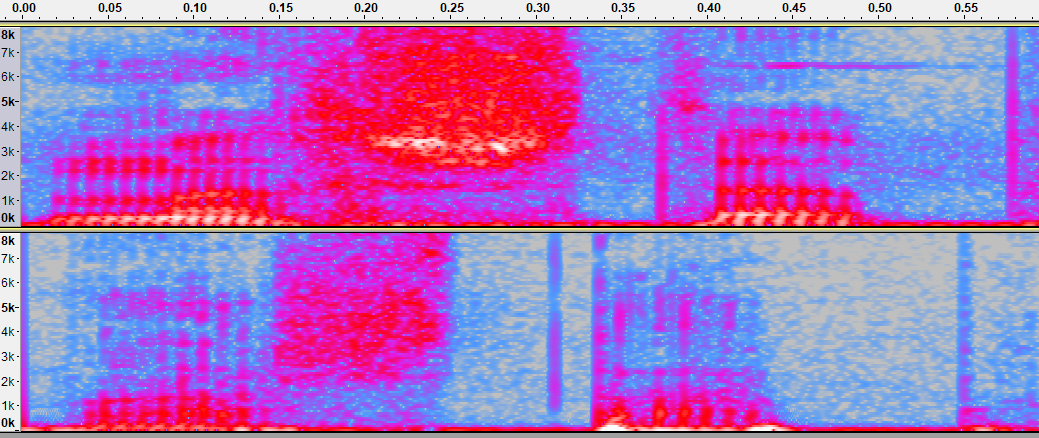
\includegraphics[width=1.0\textwidth]{words_scale.png}
	\caption{Спектрограммы слова <<масштаб>> для дикторов Д-ий (сверху) и О-ин (снизу)}
	\label{fig:words_scale}
\end{figure}

Этот рисунок иллюстрирует различие средней частоты для двух дикторов.
Исходя из полученных результатов, на записи диктора Д-ий наблюдается самое высокое значение средней частоты --- 3177 Гц, в то время как у диктора О-ин зафиксировано самое низкое значение средней частоты --- 106 Гц.
Это означает, что у диктора Д-ий по сравнению с диктором О-ин мало энергии сконцентрировано на низких частотах и много на высоких, или, другими словами, верхняя часть графика более красная, чем другого диктора.
Также это означает, что у диктора О-ин самый низкий голос из представленных дикторов, а у диктора Д-ий --- самый высокий.

Более того, стоит отметить, что частота голоса является довольно стабильной характеристикой диктора, так как её стандартное отклонение $\sigma(\nu)$ мало по сравнению со средним значением $\mu(\nu)$.
Из этого можно сделать вывод, что средняя частота является информативным показателем речи для отдельного человека.
Это свойство может быть использовано для идентификации дикторов по речи.

По результатам статистической проверки можно сделать вывод, что после выравнивания слов по амплитуде входной сигнал удовлетворяет критерию нормальности.
Поэтому дальнейшее использование алгоритмов, требующих нормальности входных данных, обосновано.

%\newpage
%============================================================================================================================

\section{Результаты проверки работоспособности алгоритма разделения слов на однородные части} \label{sect3_2}

В данном подразделе приведены эмпирические результаты работы алгоритма, описанного в подразделе \ref{sect2_2}.
Сутью эксперимента было разбиение нескольких слов на однородные части.
В качестве эталона использовались данные о границах частей, полученные экспертом посредством оценки спектрограмм записи слов с помощью визуального анализа.
Число частей и априорные положения границ, достаточно сильно отличающиеся от эталонных, заданы в качестве исходных условий.
Изначально были предприняты попытки получить численный результат задачи по оптимизации методом перебора.
Это было обусловлено его возможностью находить глобальный экстремум в том случае, если он присутствует в исследуемой области поиска.
Но в таком случае ожидаемой проблемой является ограничение вычислительной мощности современных вычислительных машин, ввиду которой время вычисления результатов увеличивается до нескольких часов при большом количестве частей.
Поэтому было продемонстрировано несколько примеров сравнения метода перебора и алгоритмов динамического программирования, представленных выше.
В ходе сравнения была установлена высокая степень сходства полученных результатов.
Ввиду чего далее был применён подход динамического программирования, способный разделять записи каждого слова на однородные части не более чем за 1 секунду.

Изучались записи команд в виде слов, длительность произнесения которых равна 0.5--1 с, а размер каждого элементарного интервала постоянный и равняется 10 мс.
В результате, разделение команд осуществлялось на 50--100 элементарных интервалов.
Частота регистрации для используемых записей была равна 22050 Гц.
Было рассмотрено разбиение слова на 3--7 частей, каждая из которых могла включать в себя от 2 до 25 интервалов.
Интервал возможного приращения границ частей находится в пределах от минус 5 до плюс 5 элементарных интервалов от изначального местонахождения границ.
Каждое слово было обработано несколько раз для различных априорных данных по расположению границ.
При этом практически отсутствовала зависимость результатов от априорных оценок при условии, что оптимальное значение находилось в области поиска.

На рисунке \ref{fig:word_1000} и в таблице \ref{tab:results_1000} отображены способы разделения слова <<тысяча>> экспертным путём и автоматическим алгоритмом.
Слово <<тысяча>> позволяет выделить 6 звуков, хорошо различимых на слух, для каждой из его букв.

\begin{figure}[h]
	\centering
	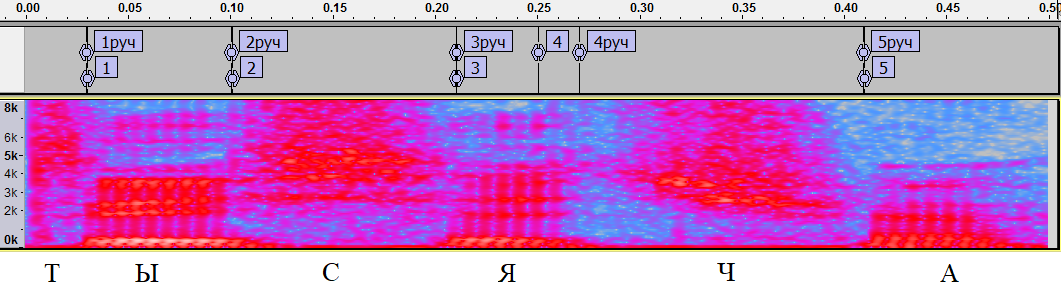
\includegraphics[width=1.0\textwidth]{word_1000.png}
	\caption{Спектрограмма слова <<тысяча>>}
	\label{fig:word_1000}
\end{figure}

\begin{table}[h]
	\centering
	\caption{Границы частей для разных критериев, слово <<тысяча>>}
	\label{tab:results_1000}
	\begin{tabular}{| l | c | c | c | c | c | c |}
		\hline
		\multirow{2}{*}{Функционал} & \multicolumn{5}{c|}{Границы частей, с} & Значение \\
		\hhline{~-----~} & \phantom{00} 1 \phantom{00} & \phantom{00} 2 \phantom{00} & \phantom{00} 3 \phantom{00} & \phantom{00} 4 \phantom{00} & \phantom{00} 5 \phantom{00} & \phantom{00}функционала\phantom{00} \\
		\hline
		$J_{1}$		& 0.03 & 0.10 & 0.21 & 0.25 & 0.41 & 0.75 \\
		$J_{2}$		& 0.03 & 0.10 & 0.21 & 0.24 & 0.41 & 0.01 \\
		$J_{3}$		& 0.03 & 0.10 & 0.21 & 0.25 & 0.41 & 0.13 \\
		$J_{12}$	& 0.03 & 0.10 & 0.21 & 0.24 & 0.41 & 0.74 \\
		$J_{123}$	& 0.03 & 0.10 & 0.21 & 0.24 & 0.41 & 0.60 \\
		\hline
		Вручную		& 0.03 & 0.10 & 0.21 & 0.27 & 0.41 & --- \\
		\hline
	\end{tabular}
\end{table}

Ручное и автоматическое разбиения слова <<больше>> показаны на рисунке \ref{fig:word_more} и представлены в таблице \ref{tab:results_more}.

\begin{figure}[h]
	\centering
 	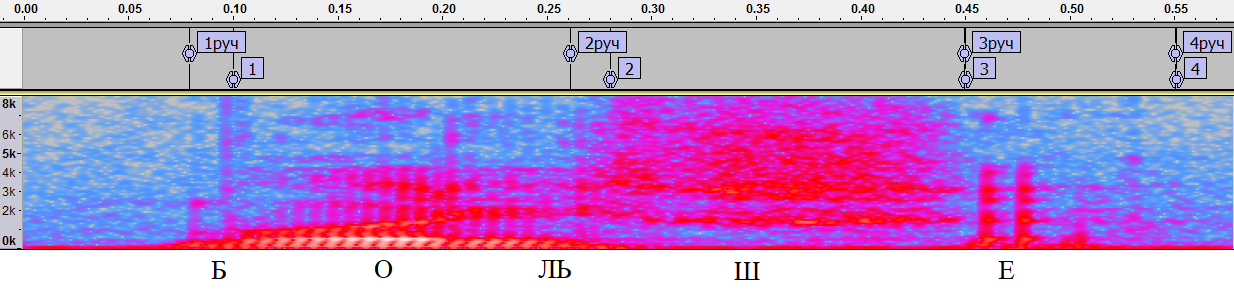
\includegraphics[width=1.0\textwidth]{word_more.png}
	\caption{Спектрограмма слова <<больше>>}
	\label{fig:word_more}
\end{figure}

\begin{table}[h]
	\centering
	\caption{Границы частей для разных критериев, слово <<больше>>}
	\label{tab:results_more}
	{\normalsize
		\begin{tabular}{| l | c | c | c | c | c | c | c | c | c | c | c |}
			\hline
			\multirow{2}{*}{Функционал} & \multicolumn{4}{c|}{Границы частей, с} & Значение \\
			\hhline{~----~} & \phantom{000} 1 \phantom{000} & \phantom{000} 2 \phantom{000} & \phantom{000} 3 \phantom{000} & \phantom{000} 4 \phantom{000} & \phantom{00}функционала\phantom{00} \\
			\hline
			$J_{1}$		& 0.10 & 0.28 & 0.45 & 0.55 & 0.54 \\
			$J_{2}$		& 0.07 & 0.28 & 0.34 & 0.37 & 0.03 \\
			$J_{3}$		& 0.10 & 0.28 & 0.45 & 0.55 & 0.15 \\
			$J_{12}$	& 0.08 & 0.28 & 0.37 & 0.55 & 0.43 \\
			$J_{123}$	& 0.08 & 0.28 & 0.38 & 0.55 & 0.27 \\
			\hline
			Вручную		& 0.08 & 0.26 & 0.45 & 0.55 & --- \\
			\hline
		\end{tabular}
	}
\end{table}

В этом слове первая часть содержит слог <<боль>>, вторая часть --- звук <<ш>> и последняя часть --- звук <<е>>.
Ввиду того, что алгоритм предназначен для нахождения однородных частей, слог <<боль>> полностью относится к первой выделенной части.
Обусловлено это тем, что маленькая длительность звука <<б>> не позволяет выделить его в отдельную часть, а звуки <<о>> и <<ль>> схожи друг с другом \cite{cooper1952some, blumstein1980perceptual}.

Ручное и автоматическое разбиения слова <<двадцать>> показаны на рисунке \ref{fig:word_20} и представлены в таблице \ref{tab:results_20}.
Слово представленное на рисунке разделялось на элементарные интервалы длиной 10 мс, и число таких интервалов получилось равным 55.

\begin{figure}[h]
	\centering
	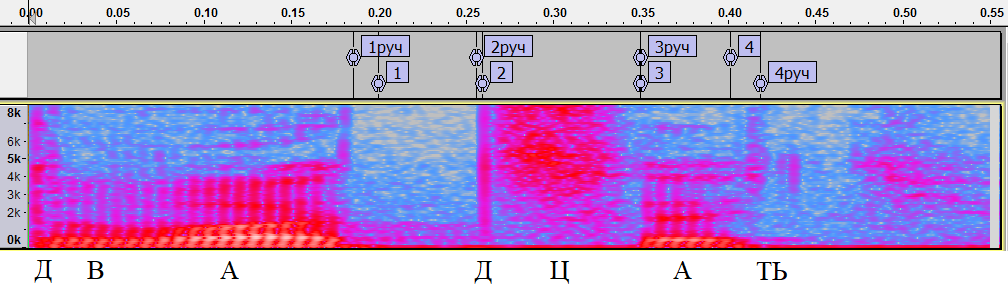
\includegraphics[width=1.0\textwidth]{word_20.png}
	\caption{Спектрограмма слова <<двадцать>>}
	\label{fig:word_20}
\end{figure}

\begin{table}[h]
	\centering
	\caption{Границы частей для разных критериев, слово <<двадцать>>}
	\label{tab:results_20}
	{\normalsize
		\begin{tabular}{| l | c | c | c | c | c | c | c | c | c | c | c |}
			\hline
			\multirow{2}{*}{Функционал} & \multicolumn{4}{c|}{Границы частей, с} & Значение \\
			\hhline{~----~} & \phantom{000} 1 \phantom{000} & \phantom{000} 2 \phantom{000} & \phantom{000} 3 \phantom{000} & \phantom{000} 4 \phantom{000} & \phantom{00}функционала\phantom{00} \\
			\hline
			$J_{1}$		& 0.20 & 0.26 & 0.35 & 0.40 & 0.67 \\
			$J_{2}$		& 0.20 & 0.26 & 0.35 & 0.39 & 0.01 \\
			$J_{3}$		& 0.20 & 0.26 & 0.35 & 0.39 & 0.15 \\
			$J_{12}$	& 0.20 & 0.26 & 0.35 & 0.40 & 0.66 \\
			$J_{123}$	& 0.20 & 0.26 & 0.35 & 0.40 & 0.51 \\
			\hline
			Вручную		& 0.18 & 0.25 & 0.35 & 0.41 & --- \\
			\hline
		\end{tabular}
	}
\end{table}

Разбиение слова <<пилотаж>> показано на рисунке \ref{fig:word_pilotage}.
В первой части слова находится звук <<п>>, во второй --- <<ило>>, после чего следует придыхание, за которым звучит <<та>> и в последней части находится звук <<ш>>.

\begin{figure}[h]
	\centering
	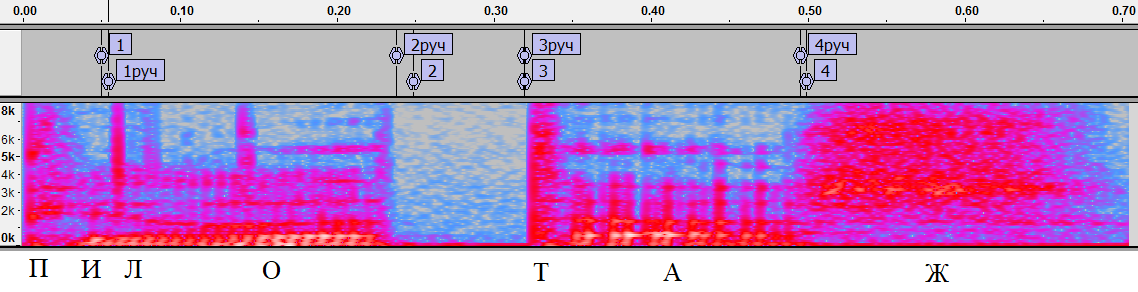
\includegraphics[width=1.0\textwidth]{word_pilotage.png}
	\caption{Спектрограмма слова <<пилотаж>>}
	\label{fig:word_pilotage}
\end{figure}

На рисунке \ref{fig:word_navigation} приведено слово <<навигация>>.
Первая часть --- это придыхание перед звуком <<н>>, далее идут части со слогами <<на>>, <<ви>> и <<га>>.
Последняя часть содержит звуки <<ция>>.

\begin{figure}[h]
	\centering
	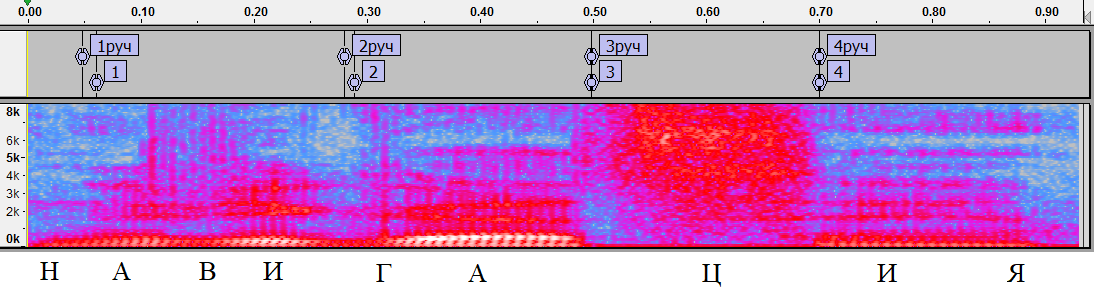
\includegraphics[width=1.0\textwidth]{word_navigation.png}
	\caption{Спектрограмма слова <<навигация>>}
	\label{fig:word_navigation}
\end{figure}

На рисунке \ref{fig:word_less} представлено слово <<меньше>>. Первая часть содержит звуки <<мень>>, затем идёт звук <<ш>> и третья часть представляет собой звук <<е>>.

\begin{figure}[h]
	\centering
	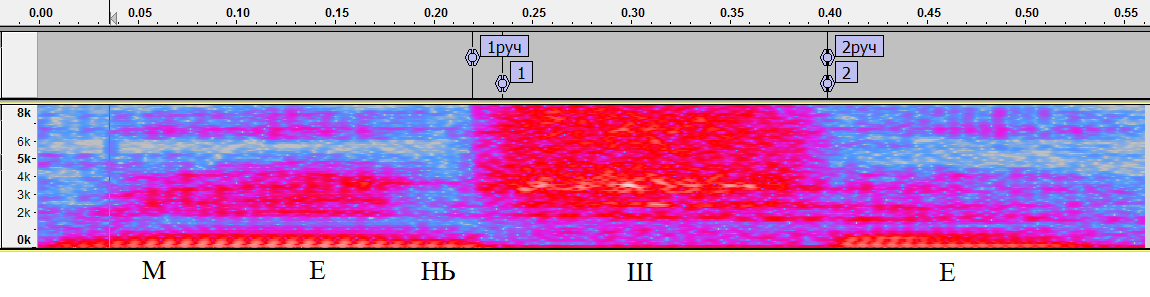
\includegraphics[width=1.0\textwidth]{word_less.png}
	\caption{Спектрограмма слова <<меньше>>}
	\label{fig:word_less}
\end{figure}

Анализ показывает достаточно хорошее совпадение границ, найденных автоматически, и эталонных границ, полученных в ручном режиме обработки.
Как правило, обнаружить различия можно во время пауз при произнесении слова.
К примеру, в слове <<двадцать>> перед <<ть>>, а в слове <тысяча>> до произнесения <<ч>>.
Проведённая обработка показывает также, что результаты, полученные при помощи различных критериев, близки между собой, особенно в тех случаях, когда однородные части содержат отдельные звуки, что соответствует допущениям, принятым при формировании критериев.
Из чего следует, что разработанные алгоритмы автоматического разделения слов на фонетически однородные части являются работоспособными.

Разработан метод автоматического разбиения слов на однородные доли по фонетическим показателям, в основе которого лежит нахождение результата с помощью многопараметрической оптимизации.
Были разработаны критерии, позволяющие воплотить принцип достижения максимального значения фонетического сходства материала в рамках одной части и значения разнородности смежных частей.
Алгоритмы, в основе которых лежит подход динамического программирования, предложены для нахождения численных результатов при решении задач с высоким быстродействием.
Адекватность принятых допущений и работоспособность данного метода были подтверждены экспериментально на примере нескольких русских слов.

По итогам выполненных экспериментов наилучшие показатели распознавания были получены при использовании первого функционала $J_1$.
К общим выводам можно отнести то, что использование простых функционалов при разбиении слов на однородные части даёт очень точное разбиение.
Сейчас получены улучшения результатов распознавания слов при использовании ручного разбиения эталона.
Использование автоматического разбиения слов также может помочь автоматизировать процесс распознавания и сократить количество ошибок.

%\newpage
%============================================================================================================================

\section{Результаты проверки работоспособности алгоритма формирования оптимального эталона на основе метода главных компонент} \label{sect3_3}

\subsection{Проверка эффективности выделения главных компонент} \label{sect3_3_1}

Проверка эффективности алгоритма выделения главных компонент на основе теории, описанной в подразделе \ref{sect2_3_1}, была выполнена следующим образом.
Анализ проводился в отдельности для каждого из трёх слов <<пилотаж>>, <<масштаб>>, <<навигация>> одного диктора.
В качестве $М$ исходных матриц \eqref{eq:2_3_1_1} были выбраны параметрические портреты всех реализаций каждого слова диктора Н-ов, то есть было составлено всего 3 различных матрицы $Х$ согласно \eqref{eq:2_3_1_2} с количеством столбцов равным 53, 44 и 53 для слов <<пилотаж>>, <<масштаб>>, <<навигация>> соответственно.

По формулам \eqref{eq:2_3_1_4} и \eqref{eq:2_3_1_5} можно вычислить первые $M'$ главных компонент, где $M'$ определяется условиями задачи. 
А оценку погрешности перехода к $M'$ главным компонентам можно рассчитать по формуле \eqref{eq:2_3_1_6}.

Сравнение, например, первой главной компоненты каждого слова с соответствующим эталоном $E$, сформированным как среднее по всем реализациям конкретного слова для выбранного диктора можно провести по формуле 

\begin{equation} \label{eq:3_3_1_1}
\epsilon_1 = \frac{||E - \widehat{k}_1 a_1 - \widehat{b}_0||}{||E||},
\end{equation}
где $||E|| = \sqrt{e_1^2 + e_2^2 + \dots + e_p^2}$ --- элементы вектора $E$ имеющего размерность $p$;

\begin{equation} \label{eq:3_3_1_2}
\widehat{k}_1 = \frac{\sum_{i=1}^p (e_i - \widehat{m}_e)(a_{1i} - \widehat{m}_{a1})}{\sum_{i=1}^p (a_{1i} - \widehat{m}_{a1})^2},	
\end{equation}

\begin{equation} \label{eq:3_3_1_3}
\widehat{b}_0 = \widehat{m}_e - \widehat{k}_1 \widehat{m}_{a1},
\end{equation}
\begin{itemize}[align=left,leftmargin=1.8em,itemindent=0pt,labelsep=0pt,labelwidth=1.8em]
	\item[где] $\widehat{m}_e = \frac{1}{p} \sum_{i=1}^p e_i$,
	\item[] $\widehat{m}_{a1} = \frac{1}{p} \sum_{i=1}^p a_{1i}$.
\end{itemize}

Формулы \eqref{eq:3_3_1_2} и \eqref{eq:3_3_1_3} есть оценки линейной парной регрессии, вычисленные по методу наименьших квадратов.

Предлагается вычислить первые $M' = 6$ главных компонент $a_1, a_2, \dots, a_6$ и проверить их на ортогональность.
Для этого нужно сформировать матрицу размерности $p \times 6$: $A_{p \times 6} = [a_1 a_2 a_3 a_4 a_5 a_6]$.
И затем вычислить матрицу размерности $6 \times 6$:

\begin{equation} \label{eq:3_3_1_4}
A_{6 \times 6} = A_{p \times 6}^T A_{p \times 6}.
\end{equation}

Если главные компоненты ортогональны, то матрица $A_{6 \times 6}$ является диагональной, то есть её недиагональные элементы на несколько порядков меньше диагональных. 

В матрицах \eqref{eq:3_3_1_5}--\eqref{eq:3_3_1_7} приведены результаты, подсчитанные по формуле \eqref{eq:3_3_1_4}.

\begin{equation} \label{eq:3_3_1_5}
A_{6 \times 6}^{\text{пилотаж}} =
\begin{bmatrix}
34765.9	& 0.0	& 0.0	& 0.0	& 0.0	& 0.0	\\
0.0		& 318.1	& 0.0	& 0.0	& 0.0	& 0.0	\\
0.0		& 0.0	& 84.5	& 0.0	& 0.0	& 0.0	\\
0.0		& 0.0	& 0.0	& 59.1	& 0.0	& 0.0	\\
0.0		& 0.0	& 0.0	& 0.0	& 41.7	& 0.0	\\
0.0		& 0.0	& 0.0	& 0.0	& 0.0	& 26.5	\\
\end{bmatrix},
\end{equation}

\begin{equation} \label{eq:3_3_1_6}
A_{6 \times 6}^{\text{масштаб}} =
\begin{bmatrix}
29516.8	& 0.0	& 0.0	& 0.0	& 0.0	& 0.0	\\
0.0		& 176.0	& 0.0	& 0.0	& 0.0	& 0.0	\\
0.0		& 0.0	& 82.3	& 0.0	& 0.0	& 0.0	\\
0.0		& 0.0	& 0.0	& 78.4	& 0.0	& 0.0	\\
0.0		& 0.0	& 0.0	& 0.0	& 63.1	& 0.0	\\
0.0		& 0.0	& 0.0	& 0.0	& 0.0	& 35.7	\\
\end{bmatrix},
\end{equation}

\begin{equation} \label{eq:3_3_1_7}
A_{6 \times 6}^{\text{навигация}} =
\begin{bmatrix}
32611.7	& 0.0	& 0.0	& 0.0	& 0.0	& 0.0	\\
0.0		& 257.3	& 0.0	& 0.0	& 0.0	& 0.0	\\
0.0		& 0.0	& 72.9	& 0.0	& 0.0	& 0.0	\\
0.0		& 0.0	& 0.0	& 56.5	& 0.0	& 0.0	\\
0.0		& 0.0	& 0.0	& 0.0	& 42.6	& 0.0	\\
0.0		& 0.0	& 0.0	& 0.0	& 0.0	& 32.7	\\
\end{bmatrix}.
\end{equation}

Внедиагональные элементы являются величинами порядка 10$^{-12}$--10$^{-14}$, что близко к ошибкам округления при скалярном перемножении векторов главных компонент.
Так как они весьма близки к нулю, можно сделать вывод, что экспериментальные данные подтверждают ортогональность главных компонент.
Также следует отметить, что скалярный квадрат первой главной компоненты на два порядка выше, чем у остальных пяти главных компонент, что свидетельствует о её весомости.

Далее разложим эталон по главным компонентам методом множественной линейной регрессии, то есть найдём оценки параметров $b_0, k_1, k_2, k_3, k_4, k_5, k_6$ соответствующие модели \eqref{eq:2_3_1_4}.	
Для этого сформируем вектор 

\begin{equation}
b = \begin{bmatrix} b_0 \\ k_1 \\ k_2 \\ k_3 \\ k_4 \\ k_5 \\ k_6 \end{bmatrix} \text{ , }
A_0 = \begin{bmatrix} 1 \\ 1 \\ \vdots \\ 1 \end{bmatrix} \text{ --- единичный вектор размерности } p
\end{equation}
и матрицу размерности $p \times 7$

\begin{equation}
A_{p \times 7} = [A_0 | A_{p \times 6}] = [A_0 A_1 A_2 A_3 A_4 A_5 A_6].
\end{equation}

Тогда все 7 оценок вектора коэффициентов разложения можно найти по формуле

\begin{equation} \label{eq:3_3_1_8}
\widehat{b} = (A_{p \times 7}^T A_{p \times 7})^{-1} A_{p \times 7}^T E.
\end{equation}

В таблицах \ref{tab:regressionCoefficientsPilotage}--\ref{tab:regressionCoefficientsNavigation} представлены коэффициенты разложения эталонов, полученных как среднее по всем реализациям каждого слова, по главным компонентам и константе.
Результаты, подсчитанные по формуле \eqref{eq:3_3_1_8}, приведены для всех трёх слов.

\begin{table}[h]
	\centering
	\caption{Коэффициенты разложения эталона по главным компонентам для слова <<пилотаж>>}
	\label{tab:regressionCoefficientsPilotage}
	\begin{tabular}{| l | c | c | c | c | c | c | c |}
		\hline
		\multicolumn{1}{|c|}{---} & \multicolumn{7}{c|}{Коэффициенты при главных компонентах} \\
		\hline
		Число гл. компонент & $\widehat{b}_0$ & $\widehat{b}_1$ & $\widehat{b}_2$ & $\widehat{b}_3$ & $\widehat{b}_4$ & $\widehat{b}_5$ & $\widehat{b}_6$ \\
		\hline
		1 гл. компонента & -0.0055 & 0.1369 & \multicolumn{1}{c|}{---} & \multicolumn{1}{c|}{---} & \multicolumn{1}{c|}{---} & \multicolumn{1}{c|}{---} & \multicolumn{1}{c|}{---} \\
		2 гл. компоненты &  0.0011 & 0.1372 & 0.0055 & \multicolumn{1}{c|}{---} & \multicolumn{1}{c|}{---} & \multicolumn{1}{c|}{---} & \multicolumn{1}{c|}{---} \\
		3 гл. компоненты &  0.0012 & 0.1372 & 0.0055 & -0.0015 & \multicolumn{1}{c|}{---} & \multicolumn{1}{c|}{---} & \multicolumn{1}{c|}{---} \\
		4 гл. компоненты &  0.0012 & 0.1372 & 0.0055 & -0.0015 & 0.0002 & \multicolumn{1}{c|}{---} & \multicolumn{1}{c|}{---} \\
		5 гл. компонент  &  0.0013 & 0.1372 & 0.0055 & -0.0015 & 0.0002 & 0.0002 & \multicolumn{1}{c|}{---} \\
		6 гл. компонент  &  0.0015 & 0.1372 & 0.0055 & -0.0015 & 0.0002 & 0.0002 & -0.0006 \\
		\hline
	\end{tabular}
\end{table}

\begin{table}[h]
	\centering
	\caption{Коэффициенты разложения эталона по главным компонентам для слова <<масштаб>>}
	\label{tab:regressionCoefficientsScale}
	\begin{tabular}{| l | c | c | c | c | c | c | c |}
		\hline
		\multicolumn{1}{|c|}{---} & \multicolumn{7}{c|}{Коэффициенты при главных компонентах} \\
		\hline
		Число гл. компонент & $\widehat{b}_0$ & $\widehat{b}_1$ & $\widehat{b}_2$ & $\widehat{b}_3$ & $\widehat{b}_4$ & $\widehat{b}_5$ & $\widehat{b}_6$ \\
		\hline
		1 гл. компонента & -0.0015 & 0.1506 & \multicolumn{1}{c|}{---} & \multicolumn{1}{c|}{---} & \multicolumn{1}{c|}{---} & \multicolumn{1}{c|}{---} & \multicolumn{1}{c|}{---} \\
		2 гл. компоненты & -0.0003 & 0.1507 & 0.0011 & \multicolumn{1}{c|}{---} & \multicolumn{1}{c|}{---} & \multicolumn{1}{c|}{---} & \multicolumn{1}{c|}{---} \\
		3 гл. компоненты &  0.0016 & 0.1507 & 0.0013 & 0.0019 & \multicolumn{1}{c|}{---} & \multicolumn{1}{c|}{---} & \multicolumn{1}{c|}{---} \\
		4 гл. компоненты &  0.0019 & 0.1507 & 0.0013 & 0.0020 & -0.0013 & \multicolumn{1}{c|}{---} & \multicolumn{1}{c|}{---} \\
		5 гл. компонент  &  0.0020 & 0.1507 & 0.0013 & 0.0020 & -0.0013 & 0.0010 & \multicolumn{1}{c|}{---} \\
		6 гл. компонент  &  0.0003 & 0.1507 & 0.0012 & 0.0017 & -0.0013 & 0.0010 & -0.0033 \\
		\hline
	\end{tabular}
\end{table}

\begin{table}[h]
	\centering
	\caption{Коэффициенты разложения эталона по главным компонентам для слова <<навигация>>}
	\label{tab:regressionCoefficientsNavigation}
	\begin{tabular}{| l | c | c | c | c | c | c | c |}
		\hline
		\multicolumn{1}{|c|}{---} & \multicolumn{7}{c|}{Коэффициенты при главных компонентах} \\
		\hline
		Число гл. компонент & $\widehat{b}_0$ & $\widehat{b}_1$ & $\widehat{b}_2$ & $\widehat{b}_3$ & $\widehat{b}_4$ & $\widehat{b}_5$ & $\widehat{b}_6$ \\
		\hline
		1 гл. компонента & 0.0021 & 0.1373 & \multicolumn{1}{c|}{---} & \multicolumn{1}{c|}{---} & \multicolumn{1}{c|}{---} & \multicolumn{1}{c|}{---} & \multicolumn{1}{c|}{---} \\
		2 гл. компоненты & 0.0022 & 0.1373 & 0.0003 & \multicolumn{1}{c|}{---} & \multicolumn{1}{c|}{---} & \multicolumn{1}{c|}{---} & \multicolumn{1}{c|}{---} \\
		3 гл. компоненты & 0.0021 & 0.1373 & 0.0003 & 0.0010 & \multicolumn{1}{c|}{---} & \multicolumn{1}{c|}{---} & \multicolumn{1}{c|}{---} \\
		4 гл. компоненты & 0.0023 & 0.1373 & 0.0003 & 0.0010 & 0.0013 & \multicolumn{1}{c|}{---} & \multicolumn{1}{c|}{---} \\
		5 гл. компонент  & 0.0025 & 0.1373 & 0.0003 & 0.0010 & 0.0013 & 0.0028 & \multicolumn{1}{c|}{---} \\
		6 гл. компонент  & 0.0014 & 0.1373 & 0.0003 & 0.0010 & 0.0012 & 0.0028 & -0.0016 \\
		\hline
	\end{tabular}
\end{table}

Количество главных компонент, участвующих в разложении, последовательно увеличивается от 1 до 6.
Опять же можно видеть, что наиболее значимым коэффициентом регрессии является коэффициент при первой главной компоненте.
При увеличении количества компонент изменение коэффициентов незначительное. 

Формула для нахождения рассогласования с эталоном в данном случае будет иметь вид:

\begin{equation} \label{eq:3_3_1_9}
\epsilon_6 = \frac{||E - \widehat{b}_0 - \widehat{k}_1 a_1 - \widehat{k}_2 a_2 - \widehat{k}_3 a_3 - \widehat{k}_4 a_4 - \widehat{k}_5 a_5 - \widehat{k}_6 a_6||}{||E||}.
\end{equation}

С практической точки зрения интересно посмотреть рассогласование разложения эталона, а также информационный критерий, вычисленный по формуле \eqref{eq:2_3_1_6}, последовательно увеличивая число главных компонент с 1 до 6.

Результаты вычислений по формуле \eqref{eq:2_3_1_6} для трёх слов представлены в таблице \ref{tab:informationMeasureDependence}.
Первая строка данной таблицы содержит меру информативности при использовании только одной главной компоненты.
Вторая строка показывает меру информативности, когда используются две первые главные компоненты, третья строка --- три первые главные компоненты и так далее.

\begin{table}[h]
	\centering
	\caption{Мера информативности при переходе системы к разному числу главных компонент (от 1 до 6)}
	\label{tab:informationMeasureDependence}
	\begin{tabular}{|l | c | c | c |}
		\hline
		\multicolumn{1}{|c|}{---} & \multicolumn{3}{c|}{$I_p$, мера информативности} \\
		\hline
		Число гл. компонент\phantom{000} & \phantom{000}пилотаж\phantom{000} & \phantom{000}масштаб\phantom{000} & \phantom{000}навигация\phantom{000} \\
		\hline
		1 гл. компонента	& 0.980	& 0.980	& 0.979	\\
		2 гл. компоненты	& 0.989	& 0.986	& 0.987	\\
		3 гл. компоненты	& 0.991	& 0.989	& 0.989	\\
		4 гл. компоненты	& 0.993	& 0.991	& 0.990	\\
		5 гл. компонент		& 0.994	& 0.993	& 0.992	\\
		6 гл. компонент		& 0.995	& 0.995	& 0.993	\\
		\hline
	\end{tabular}
\end{table}

Из этих результатов можно сделать вывод, что первая главная компонента несёт в себе порядка 98~\% имеющейся информации, а первые три главных компоненты 99~\%.
С дальнейшим увеличением числа главных компонент доля информации, содержащаяся в компонентах, увеличивается и при 6 главных компонентах достигает 99.5~\%.

В таблице \ref{tab:mismatchMeasure} представлена мера рассогласования эталона и полученного разложения на главные компоненты по формулам аналогичным формулам \eqref{eq:3_3_1_1} и \eqref{eq:3_3_1_9}.
Здесь, как и в предыдущих таблицах, количество главных компонент, участвующих в разложении, последовательно увеличивается от 1 до 6.
В результате перехода от разложения по 1 главной компоненте до 6 главных компонент относительное уменьшение меры рассогласования составляет порядка 50--80~\%.

\begin{table}[h]
	\centering
	\caption{Мера рассогласования эталона и разложения для 3 слов}
	\label{tab:mismatchMeasure}
	\begin{tabular}{|l | c | c | c | c | c | c |}
		\hline
		\multicolumn{1}{|c|}{---} & \multicolumn{6}{c|}{Мера рассогласования} \\
		\hline
		Слово \phantom{0000000} & \phantom{000}$\epsilon_1$\phantom{000} & \phantom{000}$\epsilon_2$\phantom{000} & \phantom{000}$\epsilon_3$\phantom{000} & \phantom{000}$\epsilon_4$\phantom{000} & \phantom{000}$\epsilon_5$\phantom{000} & \phantom{000}$\epsilon_6$\phantom{000} \\
		\hline
		пилотаж		& 0.0038	& 0.0008	& 0.0006	& 0.0006	& 0.0005	& 0.0005	\\
		масштаб		& 0.0013	& 0.0011	& 0.0010	& 0.0009	& 0.0008	& 0.0003	\\
		навигация	& 0.0011	& 0.0011	& 0.0010	& 0.0009	& 0.0006	& 0.0005	\\
		\hline
	\end{tabular}
\end{table}

Из данного подраздела можно сделать вывод, что использование 6 главных компонент является целесообразным, так они содержат около 99.5~\% информации о параметрическом портрете.

%\newpage
%============================================================================================================================

\subsection{Проверка работоспособности алгоритма на основе метода главных компонент} \label{sect3_3_2}

В данном подразделе приведена проверка работоспособности алгоритма на основе метода главных компонент, описанного в подразделе \ref{sect2_3_2}.
В ходе оптимизации методом покоординатного спуска, вычисление усреднённого значения нижней границы Z-коэффициента корреляции проводится с использованием обучающей выборки --- реализаций слов диктора Н-ов с шумом в наушниках 80 дБ, в то время как исходное разложение на главные компоненты было получено по записям того же диктора без шума.
Более подробно исследование информативности главных компонент в зависимости от их количества будет приведено в следующем подразделе.

Для поэтапного отслеживания эффективности работы метода покоординатного спуска ниже представлены таблицы \ref{tab:deltaZNoOptimization} и \ref{tab:deltaZOptimization}, в которых указано среднее значение и стандартное отклонение для величины $\Delta Z^{low}_{i}$, определённой в формуле \eqref{eq:2_3_2_2}, а также вероятность того, что данная величина, которая подчиняется нормальному закону распределения, будет иметь значение меньше нуля.
При этом, так как при распознавании возникает две величины $\Delta Z_{ij}$, показаны значения для наименьшей из них равной $\Delta Z^{low}_{i}$, согласно методологии, описанной в подразделе \ref{sect2_3_2}.

В таблице \ref{tab:deltaZNoOptimization} указаны результаты вычислений, применённых к тестовой выборке и изначальному эталону, полученному по формуле \eqref{eq:2_3_2_4} без выполнения оптимизации.

\begin{table}[h]
	\centering
	\caption{Статистические данные для величины $\Delta Z^{low}_{i}$, полученные при вычислении коэффициента корреляции на тестовой выборке и не оптимизированном эталоне}
	\label{tab:deltaZNoOptimization}
	\begin{tabular}{| l | c | c | c |}
		\hline
		Слово \phantom{0000000} & \phantom{000} $\mu(\Delta Z^{low}_{i})$ \phantom{000} & \phantom{000} $\sigma(\Delta Z^{low}_{i})$ \phantom{000} & \phantom{000} $P(\Delta Z^{low}_{i} < 0)$ \phantom{000} \\
		\hline
		пилотаж		& 0.789	& 0.177 & 4.25E-06 \\
		масштаб		& 1.212	& 0.221 & 2.21E-08 \\
		навигация	& 0.791	& 0.250 & 7.86E-04 \\
		\hline
	\end{tabular}
\end{table}

В таблице \ref{tab:deltaZOptimization} указаны результаты, полученные на тестовой выборке и эталоне, построенном после применения 5 циклов оптимизации.
Было проведено 5 циклов оптимизации простого варианта оптимизации коэффициентов разложения в формуле \eqref{eq:2_3_2_5}, так как сработал критерий остановки - увеличение значения нижней границы $\Delta Z^{low}_{i}$ после пятого цикла по сравнению с результатами значений четвёртого цикла менее чем на 2~\%.

\begin{table}[h]
	\centering
	\caption{Статистические данные для величины $\Delta Z^{low}_{i}$, полученные при вычислении коэффициента корреляции на тестовой выборке и оптимизированном эталоне после 5 циклов}
	\label{tab:deltaZOptimization}
	\begin{tabular}{| l | c | c | c |}
		\hline
		Слово \phantom{0000000} & \phantom{000} $\mu(\Delta Z^{low}_{i})$ \phantom{000} & \phantom{000} $\sigma(\Delta Z^{low}_{i})$ \phantom{000} & \phantom{000} $P(\Delta Z^{low}_{i} < 0)$ \phantom{000} \\
		\hline
		пилотаж		& 0.917	& 0.149	& 3.89E-10 \\
		масштаб		& 1.203	& 0.178	& 6.44E-12 \\
		навигация	& 0.743	& 0.211	& 2.20E-04 \\
		\hline
	\end{tabular}
\end{table}

Из таблиц \ref{tab:deltaZNoOptimization} и \ref{tab:deltaZOptimization} видно, что на тестовой выборке алгоритм работает корректно, так как вероятность неправильного распознавания $P(\Delta Z^{low}_{i} < 0)$ уменьшается для всех трёх слов.

Распознавание для всех 12 дикторов было осуществлено для того, чтобы удостовериться в хорошем качестве распознавания оптимизированным эталоном.
Использовались все дикторы, кроме диктора Н-ов, на записях которого производилась оптимизация коэффициентов.
При этом для распознавания применялись эталоны, использованные в начале подраздела, то есть полученные на речевых данных диктора Н-ов.
Здесь для краткости будут приведены результаты распознавания только для слова <<навигация>>.
Результаты распознавания для слова <<пилотаж>> и <<масштаб>> получились аналогичными.

В таблицах \ref{tab:deltaZ12DictorsNoOptimizatioNavigation} и \ref{tab:deltaZ12DictorsOptimizatioNavigation} последовательно приведены результаты распознавания для одного из тестируемых слов при использовании изначального неоптимизированного эталона и при использовании оптимизированного эталона.

\begin{table}[h]
	\centering
	\caption{Статистические данные для величины $\Delta Z$, полученные при вычислении коэффициента корреляции для 12 дикторов и не оптимизированном эталоне для слова <<навигация>>}
	\label{tab:deltaZ12DictorsNoOptimizatioNavigation}
	\begin{tabular}{| l | c | c | c |}
		\hline
		Номер диктора & \phantom{000} $\mu(\Delta Z^{low}_{i})$ \phantom{000} & \phantom{000} $\sigma(\Delta Z^{low}_{i})$ \phantom{000} & \phantom{000} $P(\Delta Z^{low}_{i} < 0)$ \phantom{000} \\
		\hline
		1	& 0.880	& 0.209	& 1.23E-05 \\
		2	& 0.878	& 0.256	& 3.02E-04 \\
		3	& 0.958	& 0.127	& 2.47E-14 \\
		4	& 0.870	& 0.094	& 1.01E-20 \\
		5	& 0.624	& 0.231	& 3.48E-03 \\
		6	& 0.778	& 0.209	& 9.88E-05 \\
		7	& 0.693	& 0.118	& 2.42E-09 \\
		8	& 0.522	& 0.163	& 6.95E-04 \\
		9	& 0.748	& 0.163	& 2.15E-06 \\
		10	& 0.857	& 0.129	& 1.36E-11 \\
		11	& 0.523	& 0.115	& 2.57E-06 \\
		12	& 0.841	& 0.163	& 1.24E-07 \\
		\hline
	\end{tabular}
\end{table}

\begin{table}[h]
	\centering
	\caption{Статистические данные для величины $\Delta Z$, полученные при вычислении коэффициента корреляции для 12 дикторов и оптимизированном эталоне для слова <<навигация>> }
	\label{tab:deltaZ12DictorsOptimizatioNavigation}
	\begin{tabular}{| l | c | c | c |}
		\hline
		Номер диктора & \phantom{000} $\mu(\Delta Z^{low}_{i})$ \phantom{000} & \phantom{000} $\sigma(\Delta Z^{low}_{i})$ \phantom{000} & \phantom{000} $P(\Delta Z^{low}_{i} < 0)$ \phantom{000} \\
		\hline
		1	& 0.817	& 0.196	& 1.51E-05 \\
		2	& 0.792	& 0.238	& 4.36E-04 \\
		3	& 0.768	& 0.114	& 7.03E-12 \\
		4	& 0.683	& 0.071	& 2.11E-22 \\
		5	& 0.562	& 0.225	& 6.25E-03 \\
		6	& 0.705	& 0.230	& 1.06E-03 \\
		7	& 0.739	& 0.110	& 9.43E-12 \\
		8	& 0.598	& 0.144	& 1.54E-05 \\
		9	& 0.646	& 0.146	& 5.01E-06 \\
		10	& 0.676	& 0.108	& 2.17E-10 \\
		11	& 0.443	& 0.116	& 6.45E-05 \\
		12	& 0.815	& 0.168	& 6.12E-07 \\
		\hline
	\end{tabular}
\end{table}

Представленные таблицы показывают, что при использовании оптимизированного эталона не всегда удаётся добиться улучшения распознавания слов дикторов, не входивших в обучающую выборку.
Для слова <<навигация>>, можно заметить, что ухудшение в значении вероятности неправильного распознавания произошло для 3, 6, 10 и 11 дикторов, для остальных дикторов было показано улучшение качества распознавания.

С целью проверить качественные показатели полученного эталона, кроме всего прочего, были идентифицированы реализации слов, не использовавшиеся для создания эталона и произносившиеся при проведении эксперимента с обратной связью.
То есть, в комнате через колонки подавался шум самолёта Boeing с уровнем громкости 80 дБ, а диктору, который зачитывал слова в наушники, подавался его же голос.
В таблице \ref{tab:errorsPercentageInitialOptimized} выведен процент ошибок распознавания для изначального эталона (1) и улучшенного эталона (2) соответственно для всех трёх слов.
Опять же можно увидеть, что улучшение распознавания наблюдается не для всех дикторов, но суммарное количество ошибок стало меньше.

\begin{table}[h]
	\centering
	\caption{Процент ошибок распознавания для всех трёх слов при использовании изначального (1) и оптимизированного (2) эталонов}
	\label{tab:errorsPercentageInitialOptimized}
	\begin{tabular}{| l | c | c | c | c | c | c |}
		\hline
		\multicolumn{1}{|c|}{---} & \multicolumn{6}{c|}{Процент ошибок} \\
		\hline
		\multicolumn{1}{|c|}{Номер} & \multicolumn{2}{c|}{пилотаж} & \multicolumn{2}{c|}{масштаб} & \multicolumn{2}{c|}{навигация} \\
		\hhline{~------}
		\multicolumn{1}{|c|}{\phantom{00} диктора \phantom{00}}& \phantom{00} (1) \phantom{00} & \phantom{00} (2) \phantom{00} & \phantom{00} (1) \phantom{00} & \phantom{00} (2) \phantom{00} & \phantom{00} (1) \phantom{00} & \phantom{00} (2) \phantom{00} \\
		\hline
		1		& 0	& 2	& 9	 & 18 & 9  & 6	\\
		2		& 0	& 0	& 95 & 95 & 92 & 81	\\
		3		& 0	& 2	& 68 & 66 & 6  & 8	\\
		4		& 0	& 0	& 36 & 41 & 2  & 6	\\
		5		& 0	& 0	& 0	 & 0  & 0  & 0	\\
		6		& 0	& 0	& 98 & 70 & 98 & 64	\\
		7		& 0	& 0	& 30 & 9  & 2  & 2	\\
		8		& 0	& 0	& 0	 & 0  & 4  & 4	\\
		9		& 0	& 0	& 2	 & 2  & 0  & 0	\\
		10		& 0	& 0	& 95 & 89 & 94 & 95	\\
		11		& 4	& 2	& 23 & 25 & 6  & 34	\\
		12		& 0	& 0	& 2	 & 2  & 0  & 0	\\
		\hline
		Среднее	& 0	& 0	& 38 & 35 & 26 & 24 \\
		\hline
	\end{tabular}
\end{table}

По результатам экспериментов в данном подразделе можно заметить, что оптимизация эталона в среднем помогает увеличить нижнюю границу дельты коэффициента корреляции и снизить количество ошибок распознавания.
При этом стоит отметить, что, несмотря на общее снижение количества ошибок, для определённых дикторов процент ошибок может увеличиваться.

\clearpage

%\newpage
%============================================================================================================================

\subsection{Распознавание с помощью алгоритма на основе метода главных компонент} \label{sect3_3_3}

В данном подразделе выполняется тестирование распознавания с помощью метода главных компонент, описанного в подразделе \ref{sect2_3_2}.
В качестве тестовых данных для распознавания использовались три слова: <<пилотаж>>, <<навигация>> и <<масштаб>>.
Они произнесены 4 дикторами в условиях с шумом в наушниках и 10 в условиях без шума \cite{korsun2014algo, korsun2012method, schmidt2000speech}.
По 10 различным дикторам в условиях без шума находятся 10 наборов эталонов для всех слов.
Они составляются путём обычного усреднения записей, наиболее близких по длине к среднему значению длины записи соответствующего слова.
Далее из этих усреднённых эталонов находятся 6 главных компонент, а потом проводится регрессия усреднённого эталона на константу и полученные 6 главных компонент.
В результате этого получаются коэффициенты при главных компонентах.
Далее с использованием обучающей выборки, состоящей из записей диктора Н-ов с шумом в наушниках 80 дБ, была произведена оптимизация коэффициентов при главных компонентах.

Распознавание всех команд второго набора, надиктованного 4 дикторами со значениями шума в наушниках 80 дБ и 90 дБ было проведено в качестве тестирования качества оптимизированного эталона.
Результаты представлены в таблицах \ref{tab:subsect3_3_3_tab1} и \ref{tab:subsect3_3_3_tab2}.

\begin{table}[h]
	\centering
	\caption{Результаты распознавания записей с шумом в наушниках 80 дБ на обычном (1) и оптимизированном (2) эталонах}
	\label{tab:subsect3_3_3_tab1}
	\begin{tabular}{| c | c | c | c |}
		\hline
		\phantom{000} Диктор \phantom{000} & \phantom{000000} Слово \phantom{000000} & \phantom{000} Ошибки 1 \phantom{000} & \phantom{000} Ошибки 2 \phantom{000} \\
		\hline
				& пилотаж	& 6 & 0 \\
		Б-ак	& масштаб   & 0 & 0 \\
				& навигация & 0 & 8 \\
		\hline
				& пилотаж	& 3 & 0 \\
		Г-ов	& масштаб   & 0 & 0 \\
				& навигация & 0 & 0 \\
		\hline
				& пилотаж	& 8 & 0 \\
		Н-ов	& масштаб   & 0 & 0 \\
				& навигация & 0 & 0 \\
		\hline
				& пилотаж	& 9 & 0 \\
		Ф-ев	& масштаб   & 0 & 0 \\
				& навигация & 0 & 0 \\
		\hline
		\multicolumn{2}{|c|}{Суммарные результаты} & \multicolumn{2}{c|}{\textbf{26} $\quad\longrightarrow\quad$ \textbf{8}} \\
		\hline
	\end{tabular}
\end{table}

\begin{table}[h]
	\centering
	\caption{Результаты распознавания записей с шумом в наушниках 90 дБ на обычном (1) и оптимизированном (2) эталонах}
	\label{tab:subsect3_3_3_tab2}
	\begin{tabular}{| c | c | c | c |}
		\hline
		\phantom{000} Диктор \phantom{000} & \phantom{000000} Слово \phantom{000000} & \phantom{000} Ошибки 1 \phantom{000} & \phantom{000} Ошибки 2 \phantom{000} \\
		\hline
				& пилотаж	& 7 & 0 \\
		Б-ак	& масштаб   & 0 & 0 \\
				& навигация & 0 & 1 \\
		\hline
				& пилотаж	& 3 & 0 \\
		Г-ов	& масштаб   & 0 & 0 \\
				& навигация & 0 & 2 \\
		\hline
				& пилотаж	& 12 & 0 \\
		Н-ов	& масштаб   & 0  & 0 \\
				& навигация & 0  & 0 \\
		\hline
				& пилотаж	& 4 & 0 \\
		Ф-ев	& масштаб   & 0 & 0 \\
				& навигация & 8 & 4 \\
		\hline
		\multicolumn{2}{|c|}{Суммарные результаты} & \multicolumn{2}{c|}{\textbf{34} $\quad\longrightarrow\quad$ \textbf{7}} \\
		\hline
	\end{tabular}
\end{table}

Результаты эксперимента показывают повышение качества распознавания алгоритма не только для записей слов диктора Н-ов, входящего в обучающую выборку, но и для всех остальных дикторов, при использовании оптимизированного эталона.
В распознавании было использовано 1200 записей.
Общее количество ошибок для 3 слов до оптимизации равнялось 60 или 5~\%, а после оптимизации уменьшилось до 15 или 1.25~\%.

Здесь и далее в работе будут приводиться точечные результаты оценки среднего процента правильных распознаваний.
Доверительные интервалы редко применяются при оценке результатов алгоритмов распознавания речи нескольким причинам \cite{karpov2012methodology}.
Во-первых, доверительные интервалы оказываются весьма широкими из-за большой вариативности голосов дикторов.
Во-вторых, обычно различные методы сравниваются на одинаковых тестовых базах данных записей, поэтому ширина доверительных интервалов не является информативной.
И, в-третьих, оценка доверительного интервала может оказаться ненадёжной при использовании записей одного или нескольких дикторов, так как нарушается условие независимости записей.

Кроме того, важно указать на положительные результаты распознавания при использовании неоптимизированного эталона, исходные коэффициенты разложения по главным компонентам которого были рассчитаны путём разложения усреднённого эталона.
Например, с самого начала имелась только 1 ошибка в слове <<навигация>>, произнесённого восьмым диктором.
Избавиться от данной ошибки удалось посредством оптимизации для записей без шума.

Кроме этого был проведён тест, в котором использовалось ограниченное количество реализаций слов, применяемых для получения оптимального эталона.
Результаты данных экспериментов приведены в таблице \ref{tab:subsect3_3_3_tab3}.

\begin{table}[h]
	\centering
	\caption{Результаты распознавания записей с шумом в наушниках для различного числа используемых реализаций слова и итераций при оптимизации для 3 слов}
	\label{tab:subsect3_3_3_tab3}
	{\small
		\begin{tabular}{ | l | l | l | c | c | c | c | c || c | c | c | c | c || c | c | c | c | c |}
			\hline
			\multicolumn{2}{|c|}{\textbf{\textsc{с шумом в}}} & Реализации & \multicolumn{5}{c||}{1} & \multicolumn{5}{c||}{3} & \multicolumn{5}{c|}{10} \\
			\cline{3-18}
			\multicolumn{2}{|c|}{\textbf{\textsc{\phantom{0}наушниках\phantom{0}}}} & Итерации & 0 & 1 & 3 & 10 & 30 & 0 & 1 & 3 & 10 & 30 & 0 & 1 & 3 & 10 & 30  \\
			\hline
			Диктор 	& Шум 	& Слово 	& \multicolumn{15}{c|}{Число ошибок}	\\
			\hline
					& 		& пилотаж 	& 0  & 0  & 0  & 0  & 0    & 0  & 0  & 0  & 0  & 0    & 0  & 0  & 0  & 0  & 0  \\
			Ф-ев	& 0 дБ	& масштаб 	& 0  & 0  & 0  & 0  & 0    & 0  & 0  & 0  & 0  & 0    & 0  & 0  & 0  & 0  & 0  \\
					& 		& навигация & 0  & 0  & 0  & 0  & 0    & 0  & 0  & 0  & 0  & 0    & 0  & 0  & 0  & 0  & 0  \\
			\hline
					& 		& пилотаж 	& 6  & 3  & 2  & 3  & 3    & 6  & 3  & 2  & 3  & 3    & 6  & 3  & 2  & 3  & 3  \\
			Ф-ев	& 80 дБ	& масштаб 	& 0  & 0  & 0  & 0  & 0    & 0  & 0  & 0  & 0  & 0    & 0  & 0  & 0  & 0  & 0  \\
					& 		& навигация & 0  & 0  & 0  & 0  & 0    & 0  & 0  & 0  & 0  & 0    & 0  & 0  & 0  & 0  & 0  \\
			\hline
					& 		& пилотаж 	& 1  & 1  & 0  & 0  & 0    & 1  & 1  & 0  & 0  & 0    & 1  & 1  & 0  & 0  & 0  \\
			Ф-ев  & 90 дБ	& масштаб 	& 0  & 0  & 0  & 0  & 0    & 0  & 0  & 0  & 0  & 0    & 0  & 0  & 0  & 0  & 0  \\
					& 		& навигация & 2  & 2  & 2  & 0  & 0    & 2  & 2  & 2  & 0  & 0    & 2  & 2  & 2  & 0  & 0  \\
			\hline
		\end{tabular}
	}
\end{table}

Также, вместо критерия остановки, описание которому дано в формуле \eqref{eq:2_3_2_5}, была исследована возможность применения заранее фиксированного количества итераций для оптимизации эталона.
В ходе эксперимента были использованы три тестовых выборки одного диктора с разными вариантами шума в наушниках.

Также был проведён аналогичный эксперимент, но с использованием записей других дикторов без шума.
Результаты этого эксперимента приведены в таблице \ref{tab:subsect3_3_3_tab4}.

\begin{table}[h]
	\centering
	\caption{Результаты распознавания записей с шумом в наушниках для различного числа используемых реализаций слова и итераций при оптимизации для 3 слов}
	\label{tab:subsect3_3_3_tab4}
	{\small
		\begin{tabular}{ | l | l | c | c | c | c | c || c | c | c | c | c || c | c | c | c | c |}
			\hline
			\multicolumn{1}{|c|}{\textbf{\textsc{без}}} & Реализации\phantom{0000} & \multicolumn{5}{c||}{1} & \multicolumn{5}{c||}{3} & \multicolumn{5}{c|}{10} \\
			\cline{2-17}
			\multicolumn{1}{|c|}{\textbf{\textsc{\phantom{00}шума\phantom{00}}}} & Итерации & 0 & 1 & 3 & 10 & 30 & 0 & 1 & 3 & 10 & 30 & 0 & 1 & 3 & 10 & 30 \\
			\hline
			Диктор 		& Слово 	& \multicolumn{15}{c|}{Число ошибок}	\\
			\hline
					& пилотаж 	& 0  & 0  & 0  & 0  & 0    & 0  & 0  & 0  & 0  & 0    & 0  & 0  & 0  & 0  & 0  \\
			К-ов	& масштаб 	& 0  & 0  & 0  & 0  & 0    & 0  & 0  & 0  & 0  & 0    & 0  & 0  & 0  & 0  & 0  \\
					& навигация & 7  & 5  & 0  & 0  & 0    & 7  & 5  & 0  & 0  & 0    & 7  & 5  & 0  & 0  & 0  \\
			\hline
					& пилотаж 	& 0  & 0  & 0  & 0  & 0    & 0  & 0  & 0  & 0  & 0    & 0  & 0  & 0  & 0  & 0  \\
			О-ин	& масштаб 	& 0  & 0  & 0  & 0  & 0    & 0  & 0  & 0  & 0  & 0    & 0  & 0  & 0  & 0  & 0  \\
					& навигация & 0  & 0  & 0  & 0  & 0    & 0  & 0  & 0  & 0  & 0    & 0  & 0  & 0  & 0  & 0  \\
			\hline
					& пилотаж 	& 0  & 0  & 0  & 0  & 0    & 0  & 0  & 0  & 0  & 0    & 0  & 0  & 0  & 0  & 0  \\
			С-ев	& масштаб 	& 6  & 5  & 0  & 0  & 1    & 6  & 5  & 1  & 0  & 0    & 6  & 5  & 1  & 0  & 0  \\
					& навигация & 0  & 0  & 1  & 1  & 1    & 0  & 0  & 1  & 1  & 1    & 0  & 0  & 1  & 1  & 1  \\
			\hline
					& пилотаж 	& 1  & 1  & 1  & 1  & 1    & 1  & 1  & 1  & 1  & 1    & 1  & 1  & 1  & 1  & 1  \\
			Ц-ин  	& масштаб 	& 0  & 0  & 0  & 0  & 0    & 0  & 0  & 0  & 0  & 0    & 0  & 0  & 0  & 0  & 0  \\
					& навигация & 0  & 0  & 0  & 0  & 0    & 0  & 0  & 0  & 0  & 0    & 0  & 0  & 0  & 0  & 0  \\
			\hline
		\end{tabular}
	}
\end{table}

В обоих случаев постановки эксперимента видно, что количество ошибок уменьшается с увеличением количеством итераций обучения, при этом никак не зависит от числа использованных записей.

Полученные в ходе эксперимента данные позволяют сделать вывод о том, что 1 реализации слова достаточно для вычисления оптимального эталона.
Для получения устойчивых результатов чаще всего достаточным значением являются 10 итераций, поскольку их увеличение не способствует повышению результатов.
Полученный вывод имеет большое значение в целях снижения временных затрат при оптимизации эталонов, поскольку количественное увеличение реализаций слов для получения релевантного эталона приводит к линейному росту временных затрат при работе алгоритма.

Полученный путём оптимизации коэффициентов при главных компонентах эталон продемонстрировал возможность распознавания большинства записей с существенно меньшим количеством ошибок.
Рассматриваемый алгоритм показал себя подходящим методом распознавания слов, уменьшающим число ошибок в данной задаче \cite{kolokolov2015compare}, как и алгоритм разделения слов на однородные части.
Редко встречаются случаи увеличения числа ошибок, что, скорее всего, обусловлено попаданием алгоритма в локальный, а не глобальный экстремум при использовании метода покоординатного спуска.
Ввиду этого есть смысл использовать более релевантный метод числовой оптимизации.
Также было замечено, что в качестве записей для эталона лучше использовать записи без шума, чем записи с шумом, несмотря на то что распознаваемые записи содержат шум.

Также был получен вывод о том, что для получения приемлемых результатов достаточно использовать только одну реализацию слова и проводить всего 10 итераций при получении оптимального эталона, что заметно сокращает время работы программы.

\clearpage

%\newpage
%============================================================================================================================

\section{Результаты экспериментов по формированию эталонов на основе полиномов Чебышёва} \label{sect3_4}

В данном подразделе описываются результаты экспериментов, связанных с аппроксимацией параметрических портретов полиномами Чебышёва, подробно описанной в подразделе \ref{sect2_4}.
Так как параметрический портрет представляет собой двухмерную матрицу, то аппроксимация может проводить как по временному измерению, так и по частотному.
Также можно проводить аппроксимацию по одному измерению, а затем по другому.
Наиболее оптимальным в плане уменьшения размера параметрического портрета оказалось одновременное сжатие и по частотным полосам, и по временным интервалам.

Эксперимент проводился на параметрических портретах 20 слов, произнесённых 9 различными дикторами.
При использовании исходных записей без сжатия было получено 10.7~\% ошибок при распознавании по <<чужому>> эталону и 1.6~\% ошибок при распознавании по <<своему>> эталону.
Данные результаты будут применяться для сравнения результатов распознавания после сжатия параметрических портретов распознаваемых записей.

В таблицах \ref{tab:chebyshevTest}--\ref{tab:chebyshevTrain} приведены проценты ошибок распознаваний в случае использования различного количества полиномов для обоих вариантов распознавания.

\begin{table}[h]
	\centering
	\caption{Процент ошибок при распознавании по <<чужому>> эталону для случая сжатия параметрического портрета заданным числом полиномов Чебышёва}
	\label{tab:chebyshevTest}
	\begin{tabular}{| l | c | c | c | c | c | c | c | c | c |}
		\hline
		Частотные & \multicolumn{9}{c|}{Временные интервалы} \\
		\hhline{~---------}
	 	полосы & \phantom{0} \textbf{8} \phantom{0} & \phantom{0}\textbf{10} \phantom{0} & \phantom{0}\textbf{12} \phantom{0} & \phantom{0}\textbf{14} \phantom{0} & \phantom{0}\textbf{16} \phantom{0} & \phantom{0}\textbf{18} \phantom{0} & \phantom{0}\textbf{20} \phantom{0} & \phantom{0}\textbf{22} \phantom{0} & \phantom{0}\textbf{24} \phantom{0} \\
		\hline
		\textbf{8}  & 15.7 & 16.0 & 16.5 & 16.7 & 16.8 & 16.9 & 17.1 & 17.1 & 17.1 \\
		\textbf{10} & 15.3 & 12.9 & 12.9 & 12.9 & 13.1 & 13.3 & 13.3 & 13.3 & 13.2 \\
		\textbf{12} & 15.3 & 12.8 & 11.8 & 11.9 & 11.9 & 12.0 & 12.1 & 12.1 & 12.1 \\
		\textbf{14} & 15.4 & 12.8 & 11.7 & 11.4 & 11.4 & 11.5 & 11.6 & 11.5 & 11.5 \\
		\textbf{16}	& 15.5 & 12.9 & 11.8 & 11.3 & 11.1 & 11.2 & 11.2 & 11.2 & 11.2 \\
		\textbf{18} & 15.5 & 12.8 & 11.8 & 11.3 & 11.1 & \textbf{10.9} & 10.9 & 10.8 & 10.9 \\
		\textbf{20} & 15.5 & 12.9 & 11.8 & 11.3 & 11.1 & 10.9 & 10.8 & 10.8 & 10.8 \\
		\textbf{22} & 15.4 & 12.8 & 11.8 & 11.3 & 11.1 & 10.9 & 10.8 & 10.8 & 10.8 \\
		\textbf{24} & 15.4 & 12.8 & 11.8 & 11.3 & 11.1 & 10.9 & 10.8 & 10.8 & 10.7 \\
		\hline
	\end{tabular}
\end{table}

\begin{table}[h]
	\centering
	\caption{Процент ошибок при распознавании по <<своему>> эталону для случая сжатия параметрического портрета заданным числом полиномов Чебышёва}
	\label{tab:chebyshevTrain}
	\begin{tabular}{| l | c | c | c | c | c | c | c | c | c |}
		\hline
		Частотные & \multicolumn{9}{c|}{Временные интервалы} \\
		\hhline{~---------}
	 	полосы & \phantom{0} \textbf{8} \phantom{0} & \phantom{0}\textbf{10} \phantom{0} & \phantom{0}\textbf{12} \phantom{0} & \phantom{0}\textbf{14} \phantom{0} & \phantom{0}\textbf{16} \phantom{0} & \phantom{0}\textbf{18} \phantom{0} & \phantom{0}\textbf{20} \phantom{0} & \phantom{0}\textbf{22} \phantom{0} & \phantom{0}\textbf{24} \phantom{0} \\
		\hline
		\textbf{8}  & 2.4 & 2.4 & 2.7 & 2.9 & 3.1 & 3.2 & 3.2 & 3.2 & 3.3 \\
		\textbf{10} & 2.3 & 2.1 & 2.1 & 2.2 & 2.3 & 2.4 & 2.5 & 2.5 & 2.5 \\
		\textbf{12} & 2.5 & 2.2 & 2.0 & 2.1 & 2.1 & 2.2 & 2.2 & 2.2 & 2.2 \\
		\textbf{14} & 2.6 & 2.3 & 2.0 & 1.9 & 2.0 & 2.1 & 2.1 & 2.1 & 2.0 \\
		\textbf{16} & 2.9 & 2.4 & 2.0 & 1.9 & 1.9 & 1.9 & 2.0 & 2.0 & 1.9 \\
		\textbf{18} & 2.9 & 2.6 & 2.1 & 2.0 & 2.0 & \textbf{1.8} & 1.9 & 1.9 & 1.9 \\
		\textbf{20} & 2.9 & 2.5 & 2.1 & 2.0 & 2.0 & 1.9 & 1.9 & 1.8 & 1.9 \\
		\textbf{22} & 2.9 & 2.5 & 2.2 & 2.0 & 1.9 & 1.9 & 1.8 & 1.8 & 1.8 \\
		\textbf{24} & 2.9 & 2.5 & 2.2 & 2.0 & 1.9 & 1.8 & 1.8 & 1.7 & 1.8 \\
		\hline
	\end{tabular}
\end{table}

Сначала проводилось сжатие по частотным полосам, количество полиномов указано в первом столбце.
Затем проводилось сжатие полученного портрета по временным интервалам и тут количество использованных полиномов указано в первой строке.
Эксперимент проводился для распознавания по <<чужому>> и по <<своему>> эталону.

По результатам видно, что для обоих случаев результаты совпадают в пределах приемлемой погрешности в 0.2 процентных пункта при использовании 18 полиномов в разложении по обоим измерениям.
Это позволяет уменьшить число элементов в параметрическом портрете более чем в 5 раз.
Полное совпадение количества ошибок достигается при очень большом числе полиномов, позволяя лишь незначительно уменьшить размеры параметрического портрета.

%\newpage
%============================================================================================================================

\section{Результаты проверки работоспособности алгоритмов формирования эталонов на основе формулы Байеса и метода комитетов} \label{sect3_5}

В данном подразделе приведена проверка результатов распознавания речевых команд при распознавании алгоритмом на основе формулы Байеса и метода комитетов, описанными в подразделе \ref{sect2_5}.
Проверка алгоритмом распознавания была проведена на речевой базе, включающей в себя 20 различных изолированных слов для 8 различных дикторов.
Все слова проговаривались по 30 раз.
В данном случае количественные показатели объёма речевой базы характеризуются значением 4800 для реализации слов по 600 реализаций на каждого диктора в отдельности.
Все эксперименты проводились при использовании дикторонезависимого варианта распознавания.
Это удалось реализовать посредством исключения из распознаваемых записей тех речевых записей, которые принадлежали дикторами, записи которых применялись при формировании эталона.
При распознавании применялась мера близости между матрицами параметрических портретов, представляющая собой усреднённое по столбцам Z-преобразование Фишера от коэффициентов корреляции.
В подразделе \ref{sect1_4_1} уже было дано описание данной скалярной меры близости и был расписан алгоритм её расчёта.

Результаты экспериментов представлены ниже в таблицах \ref{tab:subsect3_2_3_tab1}--\ref{tab:subsect3_2_3_tab4}.
Вариант распознавания представлен в столбце №1 каждой из таблиц.
Символ <<1\_1>> отображает распознавание по одному эталону, сформированному по аудиозаписи лишь одного диктора.
Обозначение <<1>> соответствует распознаванию с точностью до единственного слова, а обозначения <<2>> и <<3>> --- распознаванию с точностью до группы из 2 или 3 слов.
В данном случае ошибкой распознавания признается результат, при котором в группе из 2 или 3 слов с наиболее высокими показателями нельзя обнаружить истинное слово.
В последующих столбцах для всех исследуемых дикторов даны доли неправильных распознаваний в процентах от общего числа реализаций по этому диктору.
Другими словами, значение 1.00~\% соответствует 6 ошибкам.

Результаты для алгоритма на основе формулы Байеса приведены в таблице \ref{tab:subsect3_2_3_tab1} для 3 дикторов и в таблице \ref{tab:subsect3_2_3_tab2} для 7 дикторов.

\begin{table}[h]
	\centering
	\caption{Процент ошибок при распознавании алгоритмом на основе формулы Байеса по 3 эталонам}
	\label{tab:subsect3_2_3_tab1}
	\begin{tabular}{| l | c | c | c | c | c | c | c | c | c |}
		\hline
		Вариант & \multicolumn{8}{c|}{Порядковый номер диктора} & Среднее \\
		\hhline{~--------}
		распознавания & \phantom{0} 1 \phantom{0} & \phantom{0} 2 \phantom{0} & \phantom{0} 3 \phantom{0} & \phantom{0} 4 \phantom{0} & \phantom{0} 5 \phantom{0} & \phantom{0} 6 \phantom{0} & \phantom{0} 7 \phantom{0} & \phantom{0} 8 \phantom{0} & значение \\
		\hline
		$1\_1$	& 5.33 & 9.33 & 14.5 & 8.00 & 5.00 & 11.5 & 7.00 & 6.67 & 8.42 \\
		$1$		& 7.67 & 12.5 & 14.3 & 14.7 & 11.3 & 10.3 & 5.50 & 11.0 & 10.91 \\
		$2$		& 5.83 & 9.83 & 7.33 & 12.8 & 7.17 & 5.17 & 3.33 & 8.17 & 7.45 \\
		$3$		& 5.50 & 8.83 & 6.33 & 12.2 & 5.83 & 4.00 & 3.17 & 7.33 & 6.65 \\
		\hline
	\end{tabular}
\end{table}

\begin{table}[h]
	\centering
	\caption{Процент ошибок при распознавании алгоритмом на основе формулы Байеса по 7 эталонам}
	\label{tab:subsect3_2_3_tab2}
	\begin{tabular}{| l | c | c | c | c | c | c | c | c | c |}
		\hline
		Вариант & \multicolumn{8}{c|}{Порядковый номер диктора} & Среднее \\
		\hhline{~--------}
		распознавания & \phantom{0} 1 \phantom{0} & \phantom{0} 2 \phantom{0} & \phantom{0} 3 \phantom{0} & \phantom{0} 4 \phantom{0} & \phantom{0} 5 \phantom{0} & \phantom{0} 6 \phantom{0} & \phantom{0} 7 \phantom{0} & \phantom{0} 8 \phantom{0} & значение \\
		\hline
		$1\_1$	& 5.33 & 9.33 & 14.5 & 8.00 & 5.00 & 11.5 & 7.00 & 6.67 & 8.42 \\
		$1$		& 4.83 & 7.33 & 7.33 & 4.83 & 6.50 & 6.33 & 4.67 & 3.17 & 5.62 \\
		$2$		& 2.67 & 4.83 & 3.83 & 2.17 & 2.50 & 2.67 & 2.17 & 0.83 & 2.71 \\
		$3$		& 2.50 & 3.50 & 3.00 & 1.83 & 2.17 & 2.17 & 2.00 & 0.67 & 2.23 \\	
		\hline
	\end{tabular}
\end{table}

Аналогичные результаты для алгоритма на основе метода комитетов приведены в таблице \ref{tab:subsect3_2_3_tab3} для 3 дикторов и в таблице \ref{tab:subsect3_2_3_tab4} для 7 дикторов.

\begin{table}[h]
	\centering
	\caption{Процент ошибок при распознавании алгоритмом на основе метода комитетов по 3 эталонам}
	\label{tab:subsect3_2_3_tab3}
	\begin{tabular}{| l | c | c | c | c | c | c | c | c | c |}
		\hline
		Вариант & \multicolumn{8}{c|}{Порядковый номер диктора} & Среднее \\
		\hhline{~--------}
		распознавания & \phantom{0} 1 \phantom{0} & \phantom{0} 2 \phantom{0} & \phantom{0} 3 \phantom{0} & \phantom{0} 4 \phantom{0} & \phantom{0} 5 \phantom{0} & \phantom{0} 6 \phantom{0} & \phantom{0} 7 \phantom{0} & \phantom{0} 8 \phantom{0} & значение \\
		\hline
		$1\_1$			& 5.33 & 9.33 & 14.5 & 8.00 & 5.00 & 11.5 & 7.00 & 6.67 & 8.42 \\
		$1$				& 4.17 & 8.67 & 12.5 & 10.3 & 9.67 & 10.2 & 5.67 & 7.17 & 8.54 \\
		$2$				& 1.00 & 5.17 & 4.67 & 5.00 & 5.00 & 4.00 & 1.50 & 4.83 & 3.90 \\
		$3$				& 0.50 & 3.00 & 1.50 & 1.83 & 2.83 & 2.33 & 0.83 & 1.33 & 1.77 \\
		с подстройкой	& 3.20 & 6.70 & 6.30 & 7.70 & 6.30 & 5.30 & 3.30 & 5.20 & 5.50 \\
		\hline
	\end{tabular}
\end{table}

\begin{table}[h]
	\centering
	\caption{Процент ошибок при распознавании алгоритмом на основе метода комитетов по 7 эталонам}
	\label{tab:subsect3_2_3_tab4}
	\begin{tabular}{| l | c | c | c | c | c | c | c | c | c |}
		\hline
		Вариант & \multicolumn{8}{c|}{Порядковый номер диктора} & Среднее \\
		\hhline{~--------}
		распознавания & \phantom{0} 1 \phantom{0} & \phantom{0} 2 \phantom{0} & \phantom{0} 3 \phantom{0} & \phantom{0} 4 \phantom{0} & \phantom{0} 5 \phantom{0} & \phantom{0} 6 \phantom{0} & \phantom{0} 7 \phantom{0} & \phantom{0} 8 \phantom{0} & значение \\
		\hline
		$1\_1$			& 5.33 & 9.33 & 14.5 & 8.00 & 5.00 & 11.5 & 7.00 & 6.67 & 8.42 \\
		$1$				& 4.50 & 7.33 & 7.17 & 4.83 & 4.50 & 6.67 & 4.83 & 2.83 & 5.33 \\
		$2$				& 0.67 & 3.33 & 2.83 & 1.33 & 1.67 & 2.67 & 1.00 & 1.33 & 1.85 \\
		$3$				& 0.50 & 2.50 & 1.00 & 0.50 & 1.33 & 1.67 & 0.50 & 0.50 & 1.06 \\
		с подстройкой	& 1.80 & 4.50 & 4.30 & 3.20 & 1.90 & 4.80 & 2.30 & 2.20 & 3.13 \\
		\hline
	\end{tabular}
\end{table}

Из таблиц \ref{tab:subsect3_2_3_tab1} и \ref{tab:subsect3_2_3_tab3} видно, что использование 3 эталонов почти не улучшает точность по сравнению с одним (варианты <<1\_1>> и <<1>>).
Заметное улучшение в 1.5--2 раза получаем только для 7 эталонов (таблицы \ref{tab:subsect3_2_3_tab2} и \ref{tab:subsect3_2_3_tab4}, варианты <<1\_1>> и <<1>>).
При переходе к группам из 2 и 3 слов можно достичь наилучшего эффекта.
Так, для 7 эталонов по варианту <<3>> получаем в алгоритме на основе формулы Байеса долю ошибок 0.67--3.5~\% (таблица \ref{tab:subsect3_2_3_tab2}), а в алгоритме на основе метода комитетов 0.5--2.5~\% (таблица \ref{tab:subsect3_2_3_tab4}).

Следует отметить, что возможность локализации распознаваемого слова с точностью до малой группы из 2--3 слов имеет практический смысл.
Данная процедура используется в целях значительного сокращения временных затрат на распознавания команд.
Это возможно благодаря переходу к процедуре распознавания иерархическим методом, который реализуется следующим способом: в первую очередь быстродействующие алгоритмы выделяют малую группу, после чего более затратными по времени алгоритмами проводится поиск в данной группе.
К примеру, методом сравнения с эталонами <<чужих>> слов \cite{korsun2017recognition} или посредством подстройки по длительности.
В результате чего удаётся значительно уменьшить процент ошибок при распознавании.
Данный подход более подробно описан в подразделе \ref{sect2_5_6}.
Подстройка распознаваемых слов по показателю длительности использовалась только при проведении экспериментов для алгоритмов, основанных на методе комитетов, в целях экономии времени \cite{rabiner1993fundamentals, korsun2017recognition, korsun2016automatic}

Результаты распознавания, полученные с применением подстройки по времени, представлены в строках <<с подстройкой>> таблиц \ref{tab:subsect3_2_3_tab3}--\ref{tab:subsect3_2_3_tab4}.
В использованной конфигурации подстройки использовались результаты распознавания с точностью до 2 слов, так как предварительный анализ показал, что использование большего число слов не улучшает качество распознавания, при том, что значительно увеличивает время работы алгоритма.
Также в результате предварительного анализа было выявлено, что лучшие результаты достигаются при максимальном смещении границ частей на 2 шага, каждый из которых по длительности равен 2~\% от длины слова.
По результатам видно, что подстройка по времени позволяет уменьшить процент ошибок для распознавания по 3 эталонам с 8.54 до 5.50~\%.
Учитывая, что точность распознавания до 2 слов равнялась 3.90~\%, подстройка позволяет исправить две трети ошибок, допущенных алгоритмом на основе метода комитетов при выборе правильного распознавания из 2 лучших.
Аналогично, для 7 эталонов получается снижение ошибки с 5.33 до 3.13~\%, что, с учётом точности распознавания до 2 слов равной 1.85~\%, также соответствует сокращению числа ошибок на две трети.

Отметим также, что более простой эвристический алгоритм на основе метода комитетов при тестировании показал несколько лучшие результаты, чем более сложный и математически обоснованный алгоритм, использующий формулу Байеса.
Вероятнее всего, что причиной является чувствительность к неточностям оценок априорных условных вероятностей более сложного алгоритма, что и обуславливается необходимость использования более объёмных обучающих выборок.

Представлены два алгоритма, предназначенные для распознавания слов и позволяющие применять любое число эталонов.
Первый алгоритм основан на оценках априорных вероятностей, рассчитанных по обучающей выборке, а апостериорные вероятности --- по формуле Байеса.
Второй алгоритм является модификацией известного метода комитетов.
Работоспособность обоих разработанных алгоритмов подтверждается результатами тестирования.
Повышение быстродействия программ распознавания, основанных на выполнении иерархических процедур с последовательным применением алгоритмов распознавания разных видов, возможно благодаря точной локализации распознаваемого слова вплоть до малой группы, что было установлено в ходе эксперимента.

%\newpage
%============================================================================================================================

\section{Выводы по экспериментальному оцениванию характеристик распознавания предложенных алгоритмов} \label{sect3_6}

В данном разделе проведена экспериментальная проверка алгоритмов, описанных в предыдущем разделе \ref{chapt2}.
В начале описана используемая тестовая база речевых данных, она состоит из записей команд в виде слов и фраз, записанных большим количеством дикторов в условиях без шума и с шумом в наушниках.
Также отдельно имеется запись шума, накладываемая на записи команд для имитации распознавания в условиях шума.

Далее были исследованы статистические свойства речевого сигнала и параметрических портретов, определены индивидуальные особенности дикторов.
Была подтверждена гипотеза о нормальности распределения отклонений элементов параметрических портретов от эталона после выравнивания записей по амплитуде.

Следующий подраздел был посвящён проверке алгоритма автоматического разбиения слов на однородные части.
Эксперименты, проведённые на примерах нескольких слов русского языка, подтвердили работоспособность предложенного подхода и правомерность принятых допущений.
Каждый из предложенных функционалов показал качественное разбиение слов на фонетически однородные части, мало отличающееся от ручного разбиения, для всех трёх используемых слов.

После этого была проверена работоспособность алгоритма улучшения качества эталона, основанного на выделении и оптимизации главных компонент.
Было показано, что первая главная компонента содержит 98~\% информации о параметрическом портрете, а первые 6 главных компонент --- около 99.5~\%.
Существенное уменьшение процента ошибок при распознавании аудиозаписи трёх слов (с 5 до 1.25~\%) продемонстрировал эталон, который был получен посредством оптимизации коэффициентов при главных компонентах.
Кроме того, был получен вывод о целесообразности использования лишь 1 записи команды в обучающей выборке и проведения только 10 итераций подстройки при поиске приемлемого эталона для получения приемлемых результатов.
Это позволяет существенно снизить время обработки данных алгоритмом.

Также был протестирован алгоритм сжатия информации о параметрическом портрете с применением полиномов Чебышёва.
Эксперименты показали, что сжатие может происходить по частотам, по времени и по обоим измерениям одновременно.
В последнем случае можно сократить место для хранения параметрического портрета в 5--10 раз почти без ухудшения качества распознавания.	

Были проверены алгоритмы распознавания на основе формулы Байеса и метода комитетов.
Оба алгоритма позволили заметно уменьшить количество ошибок распознавания при использовании нескольких эталонов.
При использовании семи эталонов алгоритм на основе формулы Байеса позволил снизить процент ошибок при распознавании с 8.4 до 5.6~\%, а алгоритм на основе метода комитетов до 5.3~\%.
Выявленная в ходе тестирования возможность локализации распознаваемого слова с точностью до малой группы позволяет повышать быстродействие систем распознавания на основе иерархических процедур, в которых последовательно применяются алгоритмы распознавания разных видов.
Использование подстройки по времени после применения алгоритма на основе метода комитетов позволяет дополнительно снизить процент ошибок до 3.13~\%.

%\newpage
%============================================================================================================================

\clearpage           % Глава 3
\chapter{Разработка алгоритмов автоматического распознавания речевых команд на основе свёрточных нейронных сетей глубокого обучения} \label{chapt4}

В данном разделе приведено описание разработки алгоритмов автоматического распознавания речевых команд на основе свёрточных нейронных сетей глубокого обучения.
Теория по данному типу искусственных нейронных сетей описана в подразделе \ref{sect1_3_3}.
При проведении экспериментов на нейронных сетях использовались параметрические портреты меньших размеров, чем при тестировании ранее предложенными алгоритмами.
Лучшие результаты при распознавании слов были получены на портретах с 18 частотными полосами и 25 временными интервалами.
При распознавании фраз в использованных параметрических портретах также было 18 частотных полос, а число временных интервалов увеличено с 25 до 75, так как фразы в среднем состоят приблизительно из трёх слов.
В данном случае для уменьшения размерности параметрических портретов может быть использован алгоритм сжатия портретов на основе полиномов Чебышёва, описанный в подразделе \ref{sect2_4}.
Также для всех портретов из обучающей выборки может быть применено разбиение на однородные части и выравнивание найденных частей относительно друг друга для каждого слова.
Подробное описание алгоритма разбиения параметрического портрета слова на однородные части приведено в подразделе \ref{sect2_2}.

Для обучения всех нейронных сетей прямого распространения принято использовать метод обратного распространения ошибки.
Существуют пакетная, стохастическая и смешанная, мини-пакетная реализации данного метода.
Последняя реализация самая используемая на текущий момент и будет применяться в этом разделе.
К её особенностям относится некоторая случайность в процессе обучения, что приводит к немного различающимся результатам распознаваний при одинаковых параметрах обучения.
Более того, в некоторых нейронных сетях применяется регуляризация, которая также вносит небольшую случайность в процесс обучения.
Отсюда можно сделать вывод, что все результаты являются примерными и могут не воспроизводиться точь-в-точь при повторных запусках.

Моделирование искусственных нейронных сетей проводилось в программном комплексе, написанном на языке программирования Python с использованием библиотек TensorFlow и TFLearn.
TensorFlow --- это низкоуровневая библиотека с открытым исходным кодом, разработанная для решения задач построения и обучения нейронных сетей \cite{tensorflow}.
TFLearn --- высокоуровневая библиотека для упрощения работы с нейронными сетями, является оболочкой для библиотеки TensorFlow \cite{tflearn}.
Обе библиотеки могут производить вычисления как на центральном процессоре, так и на графическом процессоре.
Использование последнего является приоритетным, так как такие процессоры содержат очень много малопроизводительных ядер, что хорошо подходит для процесса обучения нейронных сетей, алгоритм которого поддаётся эффективному распараллеливанию.
Для эффективного использования графического процессора в работе программы применяется программно-аппаратная архитектура параллельных вычислений CUDA, активно использующая приведённые выше подключаемые библиотеки \cite{cuda}.

%\newpage
%============================================================================================================================

\section{Оценки работоспособности традиционных сетей типа одно- и двухслойных персептронов в задаче распознавания речевых команд} \label{sect4_1}

Первоначально в нейронных сетях были проведены оценки работоспособности традиционных сетей типа одно- и двухслойных персептронов в задаче распознавания речевых команд.
Прежде всего, исходя из стандартных рекомендаций выбиралась структура нейронной сети.
Для персептронов это количество нейронов в каждом слое.
После этого подбирались параметры сети, такие как скорость обучения, количество итераций, размер пачки и коэффициент регуляризации.
Далее, для выбранных оптимальных параметров проводилось распознавание всех записей на обучающей базе, состоящей из одного и двух дикторов.

Однослойный персептрон состоит из входного слоя, содержащего $18 \times 25 = 450$ входов (равно размеру входящего параметрического портрета) и выходного слоя, состоящего из 20 нейронов (равно количеству распознаваемых слов).
Сеть является полносвязной, то есть каждый входной элемент соединён синапсами с выходными нейронами.
Получается, что в нейронной сети есть $450 \times 20 = 9000$ синапсов или весов, которые подбираются в процессе обучения.
Для последнего слоя используется функция softmax для нормировки полученных выходных вероятностей.
Для обучения однослойного персептрона в качестве функции потерь используется перекрёстная энтропия.
В персептроне с одним слоем регуляризация обычно не применяется.
В процессе обучения используется вариант оптимизации Adam (adaptive moment estimation --- адаптивная оценка моментов) для стохастического градиентного спуска.
На рисунке \ref{fig:perceptron1_my} представлена структура полученного однослойного персептрона.

\begin{figure}[h]
	\centering
	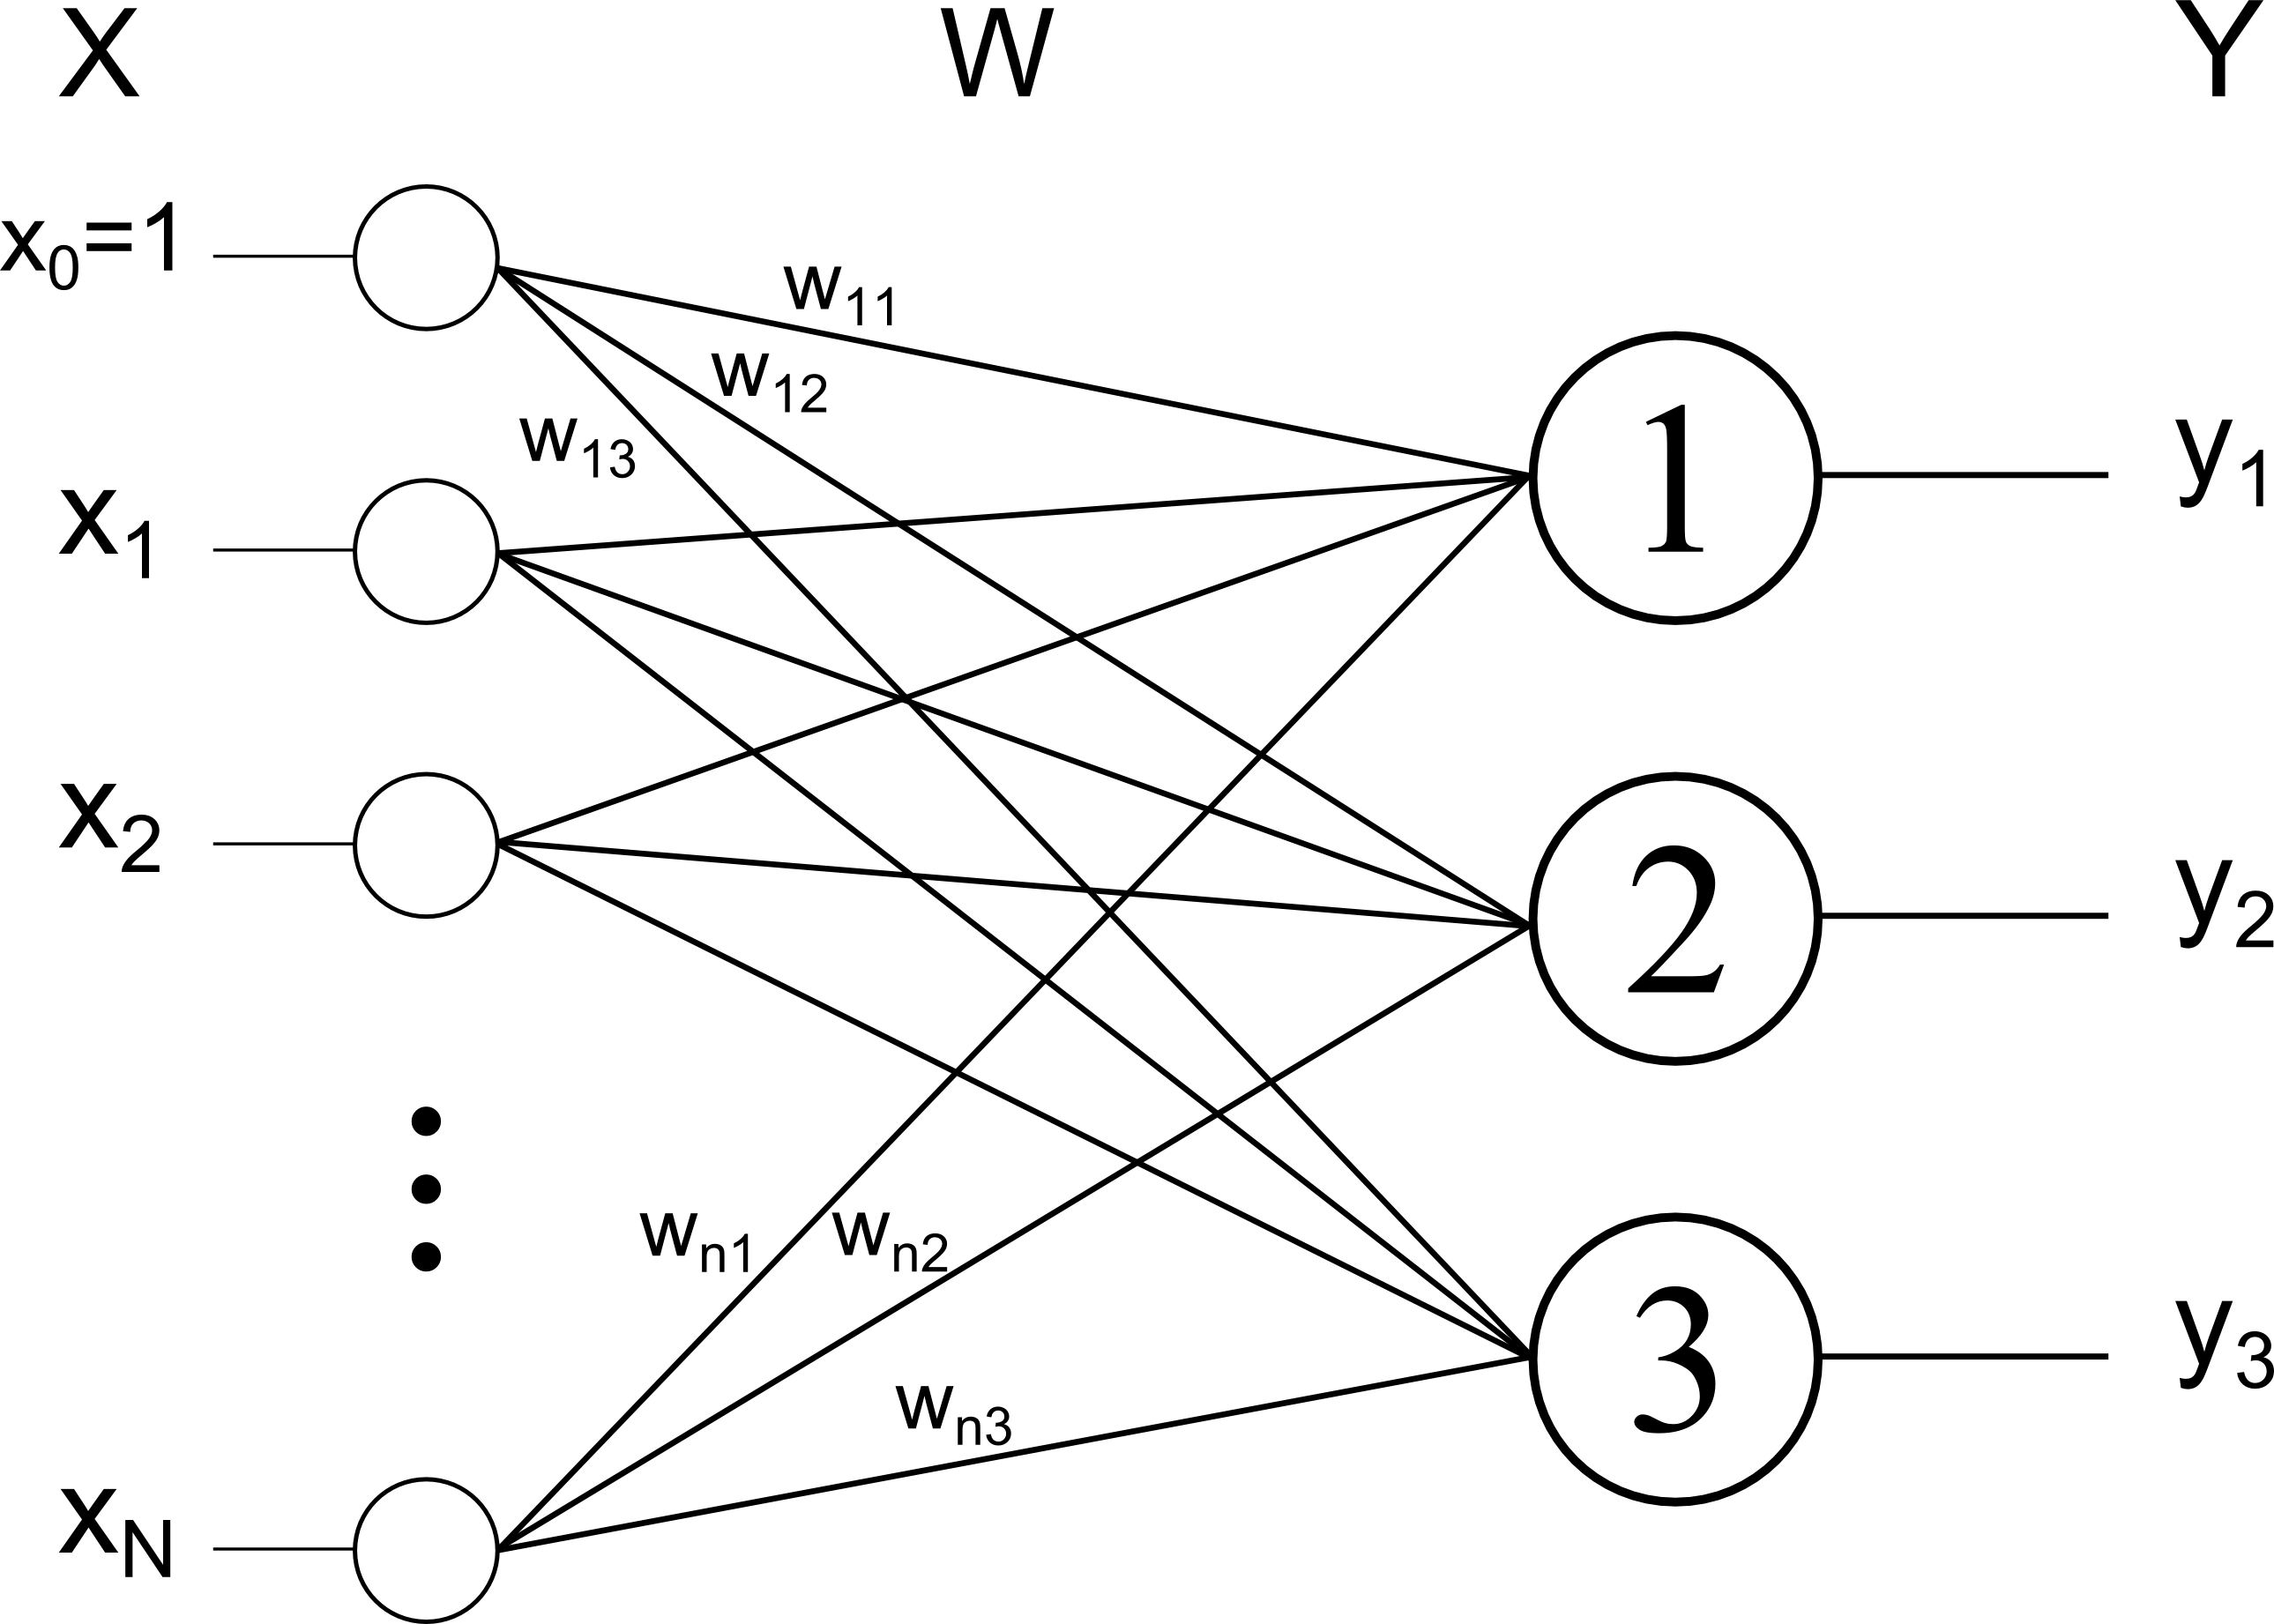
\includegraphics[width=12cm]{perceptron1_my.png}
	\caption{Структура используемого однослойного персептрона}
	\label{fig:perceptron1_my}
\end{figure}

Для однослойного персептрона сначала подбиралось количество итераций обучения и скорость обучения при фиксированном размере пачки, равному 600 записей.
Результаты подбора приведены в таблице \ref{tab:mlp1_bf_iter_pace}, оптимальное значение выделено жирным.

\begin{table}[h]
	\centering
	\caption{Подбор количества итераций и скорости обучения для однослойного персептрона, в таблице указан процент неправильных распознаваний}
	\label{tab:mlp1_bf_iter_pace}
	\begin{tabular}{| l | c | c | c | c | c | c | c | c | c |}
		\hline
		Скорость & \multicolumn{5}{c|}{Количество итераций} \\
		\hhline{~---------}
		обучения \phantom{00} & \phantom{000} 100 \phantom{000} & \phantom{000}1000\phantom{000} & \phantom{000}3000\phantom{000} & \phantom{00} 10000 \phantom{00} & \phantom{00} 30000 \phantom{00} \\
		\hline
		0.00001  & 95.68 & 93.80 & 94.36 & 91.02 & 53.87 \\
		0.00003  & 95.31 & 94.12 & 92.48 & 66.04 & 40.00 \\
		0.0001	 & 95.49 & 90.79 & 71.89 & 43.99 & 34.81 \\
		0.0003	 & 95.93 & 74.85 & 49.05 & 39.88 & 33.16 \\
		0.001  	 & 91.96 & 51.37 & 43.33 & 38.07 & 31.64 \\
		0.003 	 & 82.46 & 44.51 & 41.49 & 38.93 & 33.57 \\
		0.01 	 & 54.64 & 40.15 & 39.47 & 36.25 & 37.93 \\
		0.03 	 & 40.85 & 37.48 & 34.53 & 31.14 & 31.56 \\
		0.1 	 & 23.96 & 24.25 & \textbf{23.56} & 22.45 & 22.59 \\
		0.3 	 & 19.65 & 19.28 & 20.33 & 18.13 & 19.24 \\
		1 		 & 18.40 & 19.34 & 20.32 & 19.70 & 18.24 \\
		\hline
	\end{tabular}
\end{table}
Оптимальное количество итераций получилось равным 3000, а оптимальная скорость обучения --- 0.1.

Затем подбиралось количество итераций обучения и размер пачки при фиксированной скорости обучения, равной 0.1.
Результаты подбора приведены в таблице \ref{tab:mlp1_bf_iter_batch}, оптимальное значение выделено жирным.

\begin{table}[h]
	\centering
	\caption{Подбор количества итераций и размера пачки для однослойного персептрона, в таблице указан процент неправильных распознаваний}
	\label{tab:mlp1_bf_iter_batch}
	\begin{tabular}{| l | c | c | c | c | c | c | c | c | c |}
		\hline
		Размер	 & \multicolumn{5}{c|}{Количество итераций} \\
		\hhline{~---------}
		пачки \phantom{0000} & \phantom{000} 100 \phantom{000} & \phantom{000}1000\phantom{000} & \phantom{000}3000\phantom{000} & \phantom{00} 10000 \phantom{00} & \phantom{00} 30000 \phantom{00} \\
		\hline
		10		 & 79.16 & 79.38 & 79.92 & 79.35 & 79.12 \\
		30 		 & 61.11 & 61.85 & 61.64 & 57.45 & 58.35 \\
		60 		 & 48.60 & 44.98 & 48.23 & 46.13 & 46.12 \\
		120 	 & 36.97 & 34.37 & 37.01 & 34.99 & 34.93 \\
		200 	 & 30.00 & 31.75 & 30.22 & 26.52 & 28.96 \\
		300 	 & 27.70 & 24.25 & 27.15 & 25.85 & 28.56 \\
		450 	 & 25.34 & 25.13 & 24.23 & 22.78 & 26.93 \\
		600 	 & 24.54 & 22.16 & \textbf{23.28} & 22.81 & 25.65 \\
		\hline
	\end{tabular}
\end{table}

Оптимальное количество итераций получилось равным 3000, а оптимальный размер пачки --- 600.

Оптимальными параметрами нейронной сети стали: количество итераций обучения --- 3000, скорость обучения --- 0.1 и размер пачки 600.
Результаты распознаваний для однослойного персептрона приведены в таблице \ref{tab:mlp1_dictor1} для случая обучения на наборе данных, состоящем из записей одного диктора, и в таблице \ref{tab:mlp1_dictor2} для случая обучения на наборе данных, состоящем из записей двух дикторов.

\begin{table}[h]
	\centering
	\caption{Результаты распознавания слов однослойным персептроном на обучающем наборе из одного диктора, в таблице указан процент неправильных распознаваний}
	\label{tab:mlp1_dictor1}
	\begin{tabular}{| l | c | c | c | c | c | c | c | c | c |}
		\hline
		Набор & \multicolumn{9}{c|}{Диктор для распознавания} \\
		\hhline{~---------}
		обучения \phantom{0000} & М1    & М2    & М4    & М5    & М7    & М8    & М9    & М12   & РД \\
		\hline
		М1		 &  0.00 & 32.83 & 18.50 & 28.83 & 35.17 & 35.83 & 21.67 & 47.50 & 24.67 \\
		М2		 & 16.50 &  0.00 & 12.17 & 15.50 & 22.17 & 23.33 & 27.00 & 22.67 & 11.33 \\
		М4		 & 13.33 & 26.33 &  0.17 & 22.00 & 19.67 & 29.67 & 19.33 & 28.17 & 15.00 \\
		М5		 & 23.50 & 23.83 & 12.00 &  0.00 & 30.50 & 18.33 & 23.50 & 24.17 & 17.67 \\
		М7		 & 22.00 & 24.17 & 14.00 & 28.17 &  0.00 & 29.67 & 29.83 & 29.33 &  4.83 \\
		М8		 & 16.67 & 21.67 & 18.67 & 15.17 & 36.33 &  0.67 & 25.00 & 26.67 & 20.50 \\
		М9		 & 13.67 & 28.67 & 14.83 & 28.50 & 29.17 & 24.83 &  0.00 & 37.00 & 30.67 \\
		М12		 & 20.00 & 22.00 & 19.83 & 29.67 & 29.83 & 20.50 & 26.00 &  0.00 & 21.50 \\
		РД		 & 38.67 & 42.67 & 25.33 & 41.83 & 19.83 & 49.33 & 41.67 & 49.83 &  0.00 \\
		\hline
	\end{tabular}
\end{table}

\begin{table}[h]
	\centering
	\caption{Результаты распознавания слов однослойным персептроном на обучающем наборе из двух дикторов, в таблице указан процент неправильных распознаваний}
	\label{tab:mlp1_dictor2}
	\begin{tabular}{| l | c | c | c | c | c | c | c | c | c |}
		\hline
		Набор & \multicolumn{9}{c|}{Диктор для распознавания} \\
		\hhline{~---------}
		обучения \phantom{0000} & М1    & М2    & М4    & М5    & М7    & М8    & М9    & М12   & РД 	 \\
		\hline
		М1,М2	 &  2.50 &  4.50 & 11.50 & 22.67 & 27.00 & 19.50 & 18.00 & 25.83 & 19.67 \\
		М2,М4	 & 15.33 &  4.17 &  2.33 & 15.83 & 17.67 & 22.50 & 18.67 & 20.50 &  8.50 \\
		М4,М5	 & 14.50 & 21.00 &  2.17 &  2.83 & 21.83 & 22.33 & 21.00 & 25.33 & 16.50 \\
		М5,М7	 &  8.50 & 15.00 &  6.00 &  3.00 &  3.00 & 18.83 & 19.83 & 19.00 &  7.17 \\
		М7,М8	 & 13.83 & 13.67 & 10.00 & 12.00 &  3.50 &  5.33 & 19.67 & 15.50 &  4.50 \\
		М8,М9	 & 10.33 & 21.00 & 12.17 & 18.83 & 29.50 &  4.00 &  3.67 & 25.83 & 19.50 \\
		М9,М12	 & 14.33 & 21.00 & 14.17 & 21.50 & 24.67 & 20.50 &  3.67 &  2.50 & 17.83 \\
		М12,РД	 & 16.33 & 22.83 & 12.00 & 17.33 & 21.50 & 23.33 & 25.17 &  3.50 &  2.00 \\
		\hline
	\end{tabular}
\end{table}

Среднее количество ошибок при распознавании записей, не входящих в обучающий набор, равно 25.16~\% для первого случая и 17.84~\% для второго.

Далее рассмотрено распознавание с помощью двухслойного персептрона.
Он состоит из входного слоя, содержащего $18 \times 25 = 450$ входов (равно размеру входящего параметрического портрета), единственного скрытого слоя из 95 нейронов и выходного слоя, состоящего из 20 нейронов (равно количеству распознаваемых слов).
Количество нейронов в скрытом слое выбиралось исходя из рекомендации, согласно которой количество элементов в каждом слое должно убывать в геометрического прогрессии.
Сеть является полносвязной, то есть каждый входной элемент соединён синапсами с нейронами скрытого слоя, а каждый нейрон скрытого слоя соединён со всеми выходными нейронами.
Общее количество синапсов равно $450 \times 95 + 95 \times 20 = 44650$, веса которых нужно подобрать в процессе обучения.
По этой причине стоит использовать большее число обучающих итераций.
Для скрытого слоя используется функция активации ReLU (rectified linear unit), задаваемая уравнением $f(x) = \max (0, x)$.
Также применена регуляризация для синапсов, соединяющих скрытый слой с выходным слоем.
Аналогично однослойному персептрону, в данном случае используется функция softmax для нормировки полученных выходных вероятностей, перекрёстная энтропия в качестве функции потерь и вариант оптимизации Adam для стохастического градиентного спуска.
На рисунке \ref{fig:perceptron2_my} представлена структура полученного однослойного персептрона.

\begin{figure}[h]
	\centering
	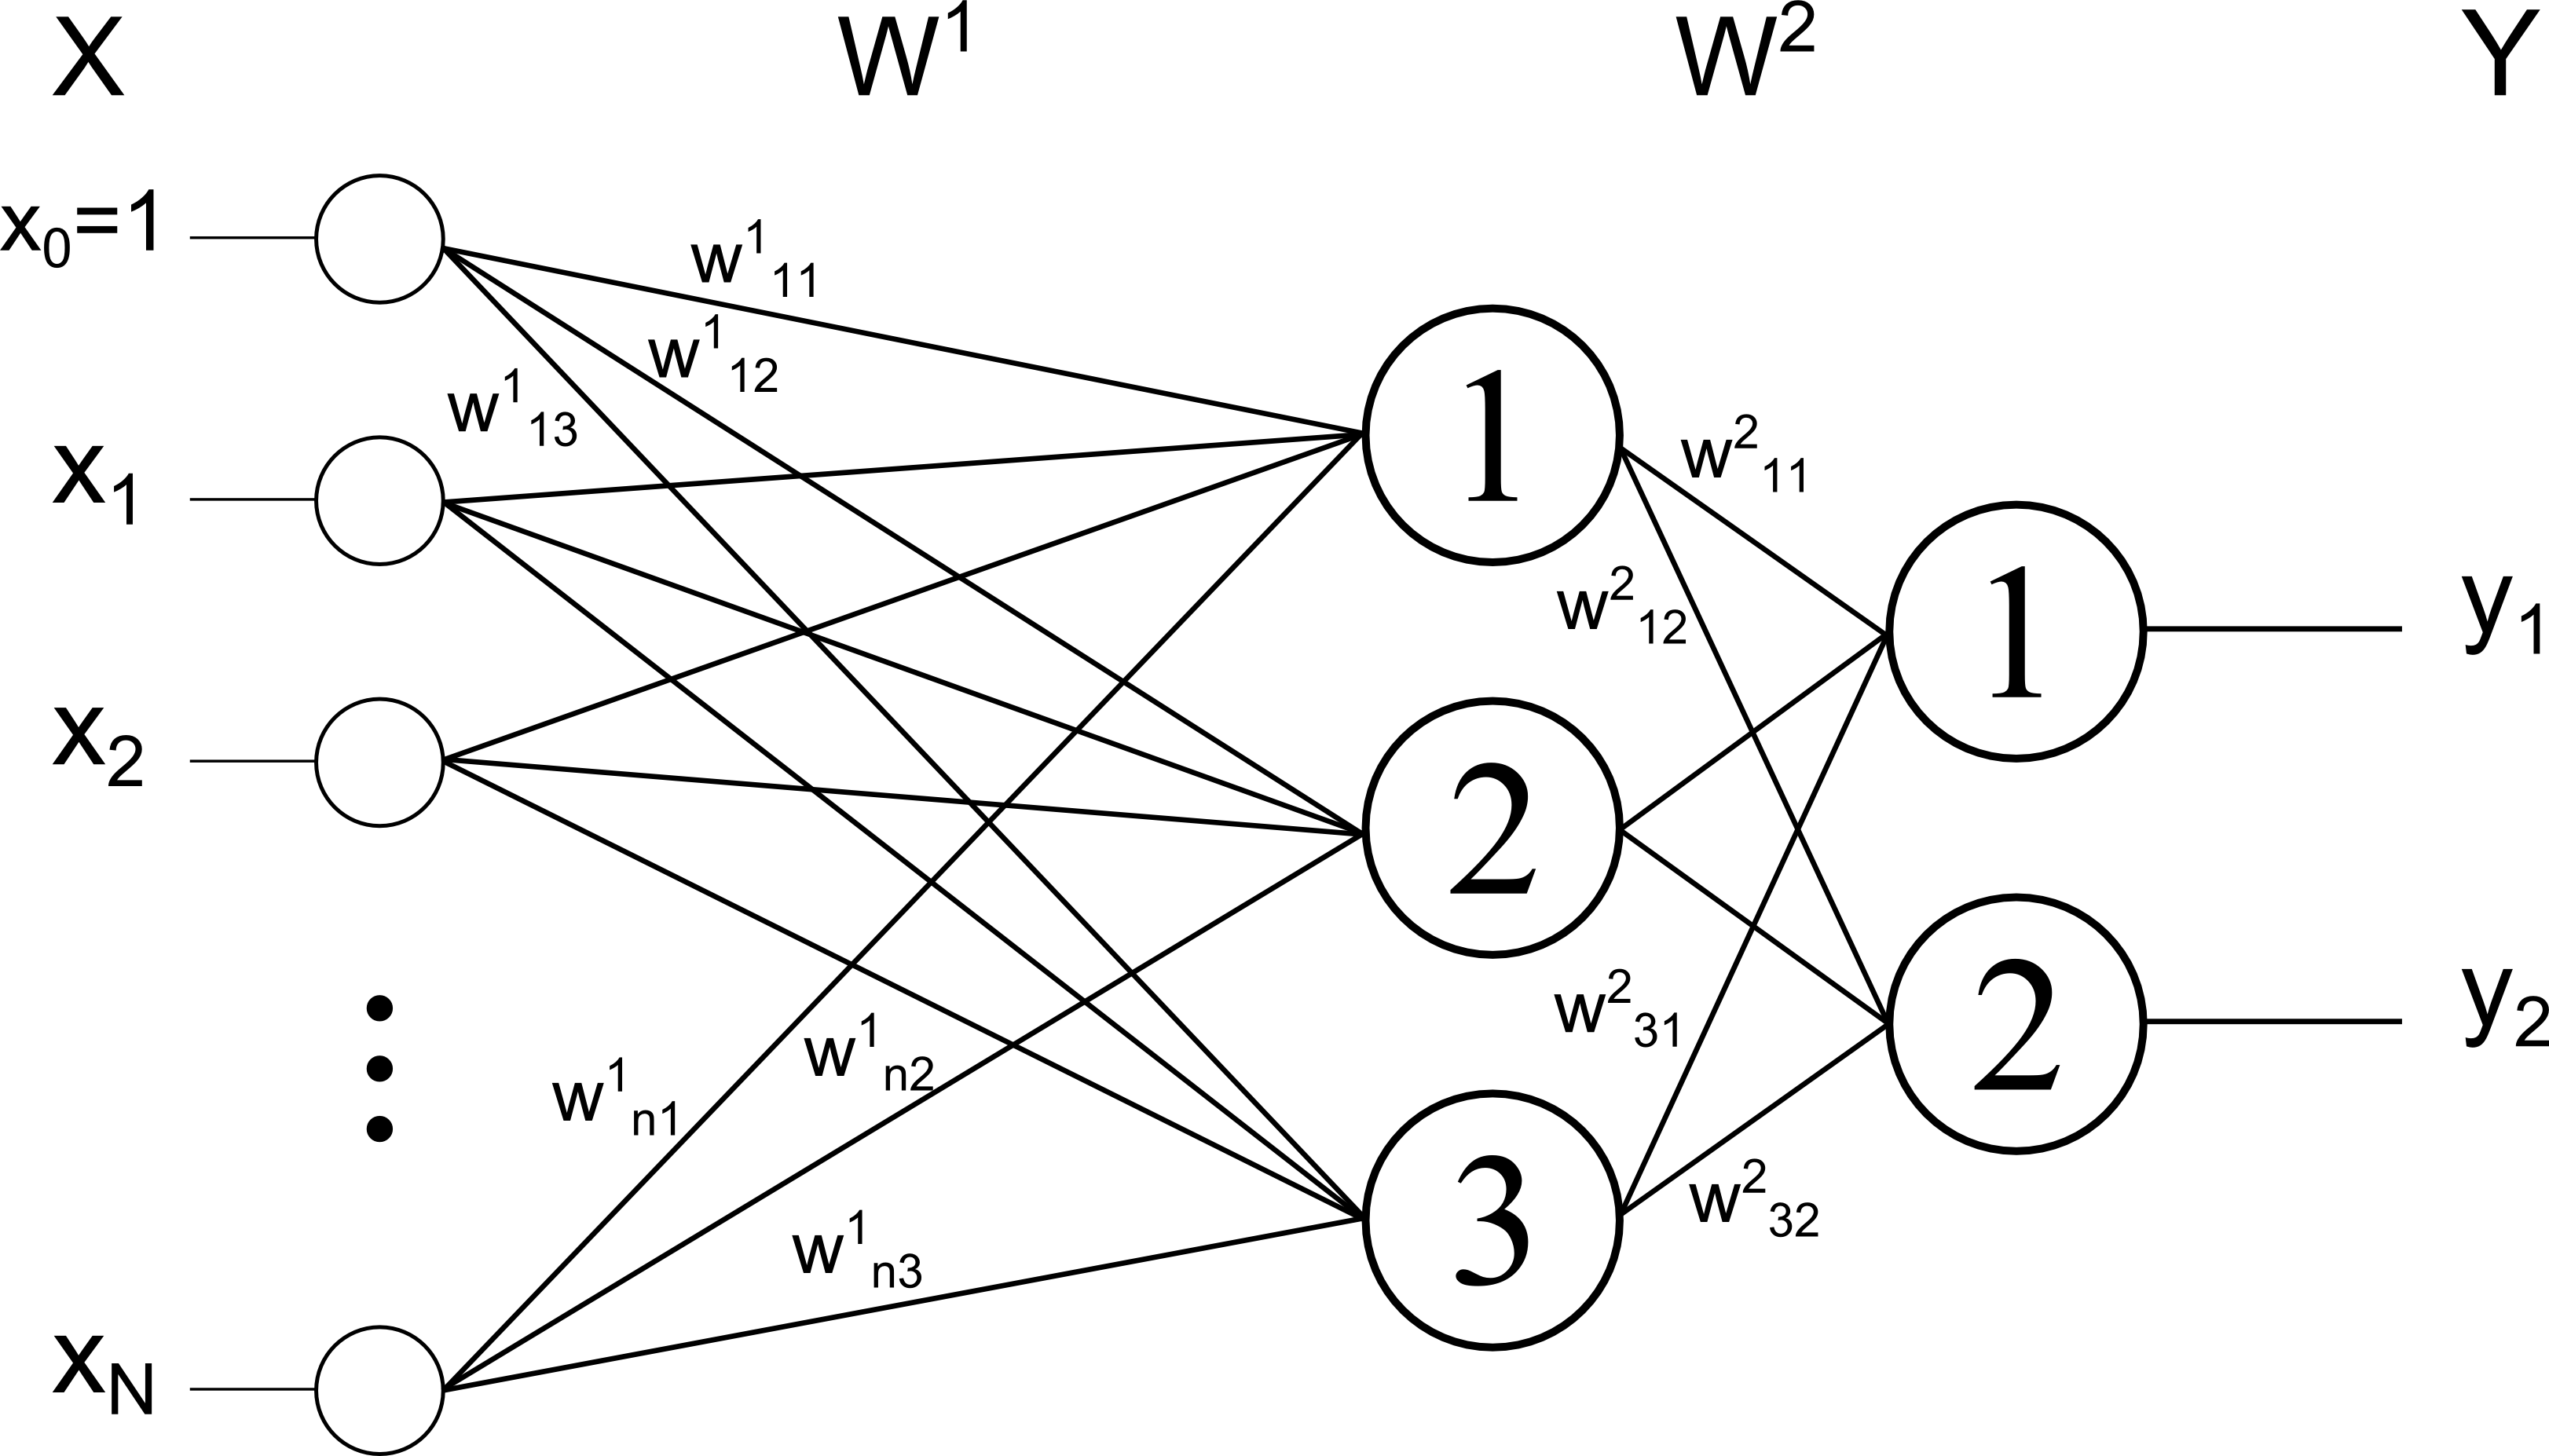
\includegraphics[width=14cm]{perceptron2_my.png}
	\caption{Структура используемого двухслойного персептрона}
	\label{fig:perceptron2_my}
\end{figure}

Для двухслойного персептрона сначала подбиралось количество итераций обучения и скорость обучения при фиксированном размере пачки, равному 600 записей.
Результаты подбора приведены в таблице \ref{tab:mlp2_bf_iter_pace}, оптимальное значение выделено жирным.

\begin{table}[h]
	\centering
	\caption{Подбор количества итераций и скорости обучения для двухслойного персептрона, в таблице указан процент неправильных распознаваний}
	\label{tab:mlp2_bf_iter_pace}
	\begin{tabular}{| l | c | c | c | c | c | c | c | c | c | c |}
		\hline
		Скорость & \multicolumn{6}{c|}{Количество итераций} \\
		\hhline{~----------}
		обучения \phantom{00} & \phantom{00} 100 \phantom{00} & \phantom{0} 1000 \phantom{0} & \phantom{0} 3000 \phantom{0} & \phantom{0} 10000 \phantom{0} & \phantom{0} 30000 \phantom{0} & \phantom{0} 100000 \phantom{0} \\
		\hline
		0.00001  & 94.72 & 95.20 & 92.48 & 77.56 & 47.65 & 37.96 \\
		0.00003  & 95.22 & 92.02 & 82.61 & 59.42 & 38.57 & 33.31 \\
		0.0001 	 & 94.45 & 82.58 & 58.62 & 39.54 & 31.09 & 25.71 \\
		0.0003	 & 93.14 & 56.03 & 46.72 & 35.81 & 30.91 & 22.67 \\
		0.001	 & 83.44 & 47.75 & 40.83 & 30.78 & \textbf{25.34} & 20.51 \\
		0.003	 & 62.90 & 51.70 & 43.55 & 28.81 & 31.67 & 31.84 \\
		0.01	 & 79.46 & 74.27 & 52.63 & 55.74 & 75.28 & 89.29 \\
		0.03	 & 94.19 & 93.45 & 91.46 & 93.58 & 94.33 & 94.16 \\
		0.1		 & 94.13 & 94.26 & 94.61 & 95.01 & 94.98 & 94.47 \\
		0.3		 & 94.43 & 94.80 & 95.03 & 95.02 & 94.87 & 94.97 \\
		1		 & 94.98 & 95.11 & 95.03 & 95.06 & 94.88 & 95.02 \\
		\hline
	\end{tabular}
\end{table}

Оптимальное количество итераций равно 30000, а оптимальная скорость обучения --- 0.001.

Затем подбиралось количество итераций обучения и коэффициент регуляризации при фиксированной скорости обучения, равной 0.001.
Результаты подбора приведены в таблице \ref{tab:mlp2_bf_iter_reg}, оптимальное значение выделено жирным.

\begin{table}[h]
	\centering
	\caption{Подбор количества итераций и коэффициента регуляризации для двухслойного персептрона, в таблице указан процент неправильных распознаваний}
	\label{tab:mlp2_bf_iter_reg}
	\begin{tabular}{| l | c | c | c | c | c | c | c | c | c | c |}
		\hline
		Коэффициент	  & \multicolumn{6}{c|}{Количество итераций} \\
		\hhline{~----------}
		регуляризации & \phantom{0} 100 \phantom{0} & \phantom{0} 1000 \phantom{0} & \phantom{0} 3000 \phantom{0} & \phantom{0} 10000 \phantom{0} & \phantom{0} 30000 \phantom{0} & \phantom{0} 100000 \phantom{0} \\
		\hline
		0.3			  & 89.67 & 92.68 & 87.50 & 79.63 & 79.77 & 77.44 \\
		0.4			  & 85.86 & 88.99 & 83.71 & 71.69 & 66.40 & 66.41 \\
		0.5			  & 85.46 & 87.27 & 84.37 & 65.18 & 56.98 & 56.42 \\
		0.6			  & 85.40 & 86.56 & 78.40 & 59.11 & 52.15 & 48.66 \\
		0.7			  & 83.28 & 80.97 & 78.42 & 51.52 & 42.78 & 38.91 \\
		0.8			  & 80.65 & 72.03 & 67.75 & 42.64 & 36.27 & 32.67 \\
		0.9			  & 83.71 & 46.72 & 41.38 & 33.38 & \textbf{23.30} & 20.03 \\
		1.0			  & 85.23 & 51.60 & 48.78 & 46.84 & 48.14 & 40.41 \\
		\hline
	\end{tabular}
\end{table}

Оптимальное количество итераций равно 30000, а оптимальный коэффициент регуляризации --- 0.9.

Оптимальными параметрами нейронной сети стали: количество итераций обучения --- 30000, скорость обучения --- 0.001, размер пачки 600 и коэффициент регуляризации --- 0.9.
Результаты распознаваний для двухслойного персептрона приведены в таблице \ref{tab:mlp2_dictor1} для случая обучения на наборе данных, состоящем из записей одного диктора, и в таблице \ref{tab:mlp2_dictor2} для случая обучения на наборе данных, состоящем из записей двух дикторов.

\begin{table}[h]
	\centering
	\caption{Результаты распознавания слов двухслойным персептроном на обучающем наборе из одного диктора, в таблице указан процент неправильных распознаваний}
	\label{tab:mlp2_dictor1}
	\begin{tabular}{| l | c | c | c | c | c | c | c | c | c |}
		\hline
		Набор & \multicolumn{9}{c|}{Диктор для распознавания} \\
		\hhline{~---------}
		обучения \phantom{0000} & М1      & М2    	 & М4      & М5    	 & М7      & М8    	 & М9      & М12   	 & РД \\
		\hline
		М1		 &  0.00 & 28.00 & 18.50 & 31.83 & 39.50 & 24.83 & 12.83 & 46.00 & 31.33 \\
		М2		 & 38.67 &  0.33 & 34.67 & 33.83 & 43.50 & 36.17 & 38.67 & 31.83 & 35.33 \\
		М4		 & 13.83 & 17.17 &  0.17 & 15.33 & 15.50 & 24.67 & 15.33 & 22.33 &  9.50 \\
		М5		 & 12.50 & 19.33 &  7.33 &  0.00 & 18.50 & 22.00 & 17.67 & 16.50 & 11.17 \\
		М7		 & 28.33 & 34.33 & 12.67 & 33.33 &  0.00 & 62.83 & 39.50 & 48.00 &  3.67 \\
		М8		 & 15.67 & 18.00 & 18.33 & 22.83 & 34.50 &  0.83 & 20.17 & 25.00 & 18.17 \\
		М9		 & 10.00 & 26.00 & 15.50 & 27.50 & 30.00 & 22.67 &  0.00 & 29.33 & 25.33 \\
		М12		 & 37.50 & 23.67 & 38.83 & 35.50 & 33.17 & 28.83 & 38.00 &  0.00 & 27.00 \\
		РД		 & 32.83 & 36.00 & 23.17 & 38.67 & 15.67 & 43.83 & 42.67 & 41.83 &  0.00 \\
		\hline
	\end{tabular}
\end{table}

\begin{table}[h]
	\centering
	\caption{Результаты распознавания слов двухслойным персептроном на обучающем наборе из двух дикторов, в таблице указан процент неправильных распознаваний}
	\label{tab:mlp2_dictor2}
	\begin{tabular}{| l | c | c | c | c | c | c | c | c | c |}
		\hline
		Набор & \multicolumn{9}{c|}{Диктор для распознавания} \\
		\hhline{~---------}
		обучения \phantom{0000} & М1      & М2    	 & М4      & М5    	 & М7      & М8    	 & М9      & М12   	 & РД \\
		\hline
		М1,М2	 &  3.00 &  3.83 & 17.83 & 24.83 & 34.50 & 21.17 & 25.50 & 40.33 & 31.50 \\
		М2,М4	 &  7.83 &  4.83 &  3.33 & 20.50 & 21.50 & 17.17 & 13.17 & 27.33 & 17.83 \\
		М4,М5	 & 18.17 & 21.33 &  2.33 &  1.83 & 23.50 & 17.33 & 18.17 & 21.33 & 16.83 \\
		М5,М7	 & 14.00 & 13.50 &  7.33 &  2.50 &  3.00 & 18.50 & 21.67 & 18.33 & 11.00 \\
		М7,М8	 & 12.00 & 19.83 &  9.50 & 16.17 &  2.83 &  5.17 & 20.83 & 16.67 &  4.17 \\
		М8,М9	 &  7.17 & 17.67 &  7.50 & 10.33 & 28.00 &  1.83 &  2.33 & 16.33 & 21.83 \\
		М9,М12	 & 13.17 & 26.33 & 14.00 & 20.17 & 25.17 & 21.83 &  4.00 &  3.67 & 14.83 \\
		М12,РД	 & 19.33 & 15.83 & 16.00 & 15.33 & 15.17 & 19.67 & 25.33 &  2.33 &  0.33 \\
		\hline
	\end{tabular}
\end{table}

Среднее количество ошибок при распознавании записей, не входящих в обучающий набор, равно 26.99~\% для первого случая и 18.43~\% для второго.

В итоге, можно сказать, что одно- и двухслойные персептроны показали неудовлетворительные результаты распознавания, с количеством ошибок в несколько раз больше, чем в ранее приведённых алгоритмах.
Далее в разделе будут рассмотрены более подходящие алгоритмы.

\clearpage

%\newpage
%============================================================================================================================

\section{Разработка структур свёрточных сетей глубокого обучения для распознавания речевых команд} \label{sect4_2}

После этого происходил выбор новых архитектур искусственных нейронных сетей, преимущественно среди рекуррентных сетей и сетей глубокого обучения, которые наиболее подходят для задач распознавания речи.
Выбраны свёрточные нейронные сети глубокого обучения.

Итоговая используемая архитектура имеет по 2 слоя свёртки и подвыборки, за которыми идут 3 полносвязных слоя.
Между полносвязными слоями производится регуляризация, состоящая в случайном выбрасывании определённого количества нейронов в процессе обучения.
Такой приём, также, как и в случае многослойных персептронов, улучшает работу сети, предотвращает переобучение и повышает стабильность результатов.
Структура нейронной сети представлена на рисунке \ref{fig:cnn_my}.

\begin{figure}[h]
	\centering
	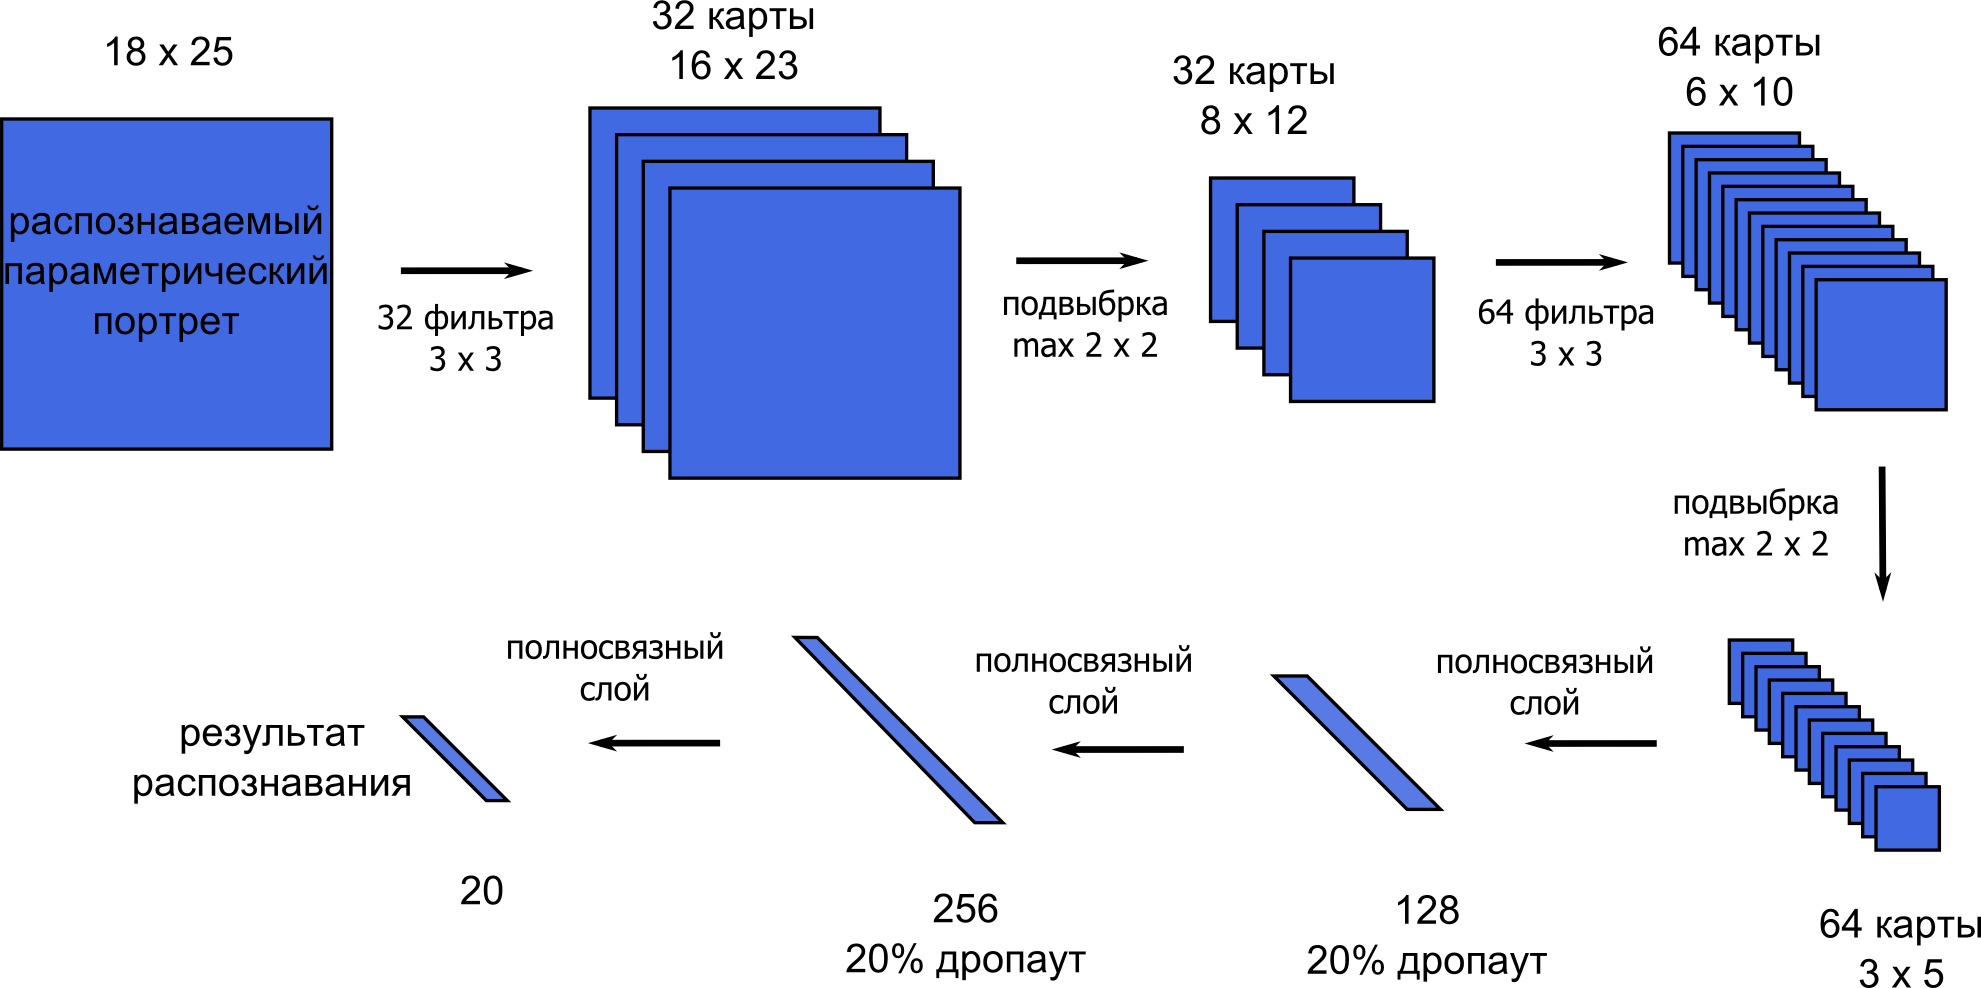
\includegraphics[width=1.0\textwidth]{cnn_my.png}
	\caption{Архитектура используемой свёрточной нейронной сети}
	\label{fig:cnn_my}
\end{figure}

Входной массив является двумерным параметрическим портретом.
Теперь, в отличии от однослойных и многослойных персептронов, нет необходимости преобразовывать двумерный параметрический портрет в одномерный массив.
Далее идёт свёрточный слой с 32 свёрточными фильтрами размером $3 \times 3$.
Затем следует слой подвыборки с размером ядра 2, то есть каждый участок каждой карты признаков размером $2 \times 2$ преобразуется в один элемент в новой карте признаков.
После этого идёт свёрточный слой с 64 фильтрами, каждый из которых применяется ко всем картам признаков и на выходе этого слоя получается 64 карты признаков.
Далее ещё один слой подвыборки с размером ядра 2, за которым идут три полносвязных слоя со 128, 256 и 20 элементами соответственно, где 20 --- это количество распознаваемых слов.
Таким образом, общее количество параметров данной нейронной сети равно $(3 \times 3 \times 1 + 1) \times 32 + (3 \times 3 \times 32 + 1)  \times 64 + (64 \times 3 \times 5 + 1) \times 128 + (128 + 1) \times 256 + (256 + 1) \times 20 = 179 988$.

В свёрточных слоях, также, как и многослойных персепронах, используется функция активации ReLU.
В первых двух полносвязных слоях используется гиперболический тангенс в качестве функции активации, который задаётся уравнением $f(x) = \tanh(x) = \frac{e^x - e^{-x}}{e^x + e^{-x}}$.
Также, после обоих скрытых полносвязных слоев применяется регуляризация для предотвращения переобучения сети.
Для последнего полносвязного слоя используется функция softmax для нормировки полученных выходных вероятностей.
Для обучения данного типа нейронных сетей в качестве функции потерь используется перекрёстная энтропия.
В процессе обучения используется вариант оптимизации Adam для стохастического градиентного спуска.

Приведённые выше количество и размеры фильтров, а также размеры финальных полносвязных слоев взяты из эмпирических рекомендаций для распознавания изображений свёрточными нейронными сетями.
Параметрический портрет является своего рода изображением, поэтому было решено использовать аналогичные параметры.

Важным является вопрос использования свёрточных нейронных сетей для малых обучающих выборок, размер которых в нашем случае будет составлять от 300 до 4900 записей.
Также стоит отметить небольшое количество классов: 20 для распознавания слов и 11 для распознавания фраз.
При этом количество элементов каждого класса в обучающей выборке не меньше 30.

Хотя изначально свёрточные нейронные сети обучались на больших выборках, в последнее время были получены обнадёживающие результаты на обучающих выборках небольшого размера.
Например, в работе \cite{dieleman2015classifying} использовалось 27000 элементов из 121 несбалансированного класса для распознавания изображений, а в работе \cite{truong2018lightweight} была использована база данных CIFAR-10 \cite{cifar10} c 50000 элементами из 10 классов в обучающей выборке.
При этом, при соблюдении определённых условий свёрточные нейронные сети показывают хорошие результаты при обучении на маленьких выборках, размером 100--1000 элементов, даже при количестве обучаемых параметров порядка нескольких сотен тысяч \cite{beam2017cnn}.
Количество обновлений градиента на одной итерации равно числу элементов в обучающей выборке, следовательно, необходимо уделить особое внимание количеству итераций и убедиться в сходимости процесса обучения.
Рекомендуется использовать функцию активации ReLU для более быстрого схождения процесса обучения и различные способы регуляризации для предотвращения переобучения.
Все указанные рекомендации были применены в используемой свёрточной нейронной сети, что даёт позволило надеяться на хороший результат.

Был произведён подбор параметров модели и выбор оптимальной сети на небольшой обучающей выборке при распознавании фраз вне этой выборки.
Подбирались оптимальные значения для количества итераций обучения и скорость обучения при фиксированном размере пачки, равному 600 записей.
Результаты подбора приведены в таблице \ref{tab:cnn_bf_iter_pace}, оптимальное значение выделено жирным.

\begin{table}[h]
	\centering
	\caption{Подбор количества итераций и скорости обучения для свёрточной нейронной сети при распознавании слов, в таблице указан процент неправильных распознаваний}
	\label{tab:cnn_bf_iter_pace}
	\begin{tabular}{| l | c | c | c | c | c | c |}
		\hline
		Скорость & \multicolumn{5}{c|}{Количество итераций} \\
		\hhline{~-----}
		обучения \phantom{00} & \phantom{000} 100 \phantom{000} & \phantom{000}1000\phantom{000} & \phantom{000}3000\phantom{000} & \phantom{00} 10000 \phantom{00} & \phantom{00} 30000 \phantom{00} \\
		\hline
		0.00001	& 70.70 & 22.60 & 13.50 &  9.50 &  7.50 \\
		0.00003	& 42.10 & 13.20 &  9.00 &  7.10 &  6.50 \\
		0.0001	& 28.50 &  9.20 &  7.20 &  6.30 &  6.00 \\
		0.0003	& 20.60 &  7.70 &  6.50 & \textbf{5.30} &  6.10 \\
		0.001	& 44.00 &  8.40 &  8.10 &  8.30 &  8.80 \\
		0.003	& 84.00 & 10.80 &  9.10 & 11.70 & 11.20 \\
		0.01	& 94.20 & 52.90 & 43.20 & \multicolumn{1}{c|}{---} & \multicolumn{1}{c|}{---} \\	
		0.03	& 95.10 & 94.90 & 94.90 & \multicolumn{1}{c|}{---} & \multicolumn{1}{c|}{---} \\	
		0.1		& 95.00 & 95.00 & 95.00 & \multicolumn{1}{c|}{---} & \multicolumn{1}{c|}{---} \\
		\hline
	\end{tabular}
\end{table}

Оптимальными параметрами нейронной сети стали: количество итераций обучения --- 10000, скорость обучения --- 0.0003 и размер пачки 600.
Результаты распознаваний для свёрточной нейронной сети на одном и нескольких дикторах приведены ниже.

%\newpage
%============================================================================================================================

\section{Экспериментальное оценивание характеристик распознавания свёрточной нейронной сети глубокого обучения} \label{sect4_3}

Проведён следующий эксперимент.
Записи каждого диктора разбивались на 2 части.
На первой части обучалась свёрточная нейронная сеть, а вторая часть использовалась в качестве тестовой выборки.
Результаты этих распознаваний приведены на рисунке \ref{fig:cnn_words_self}.
В столбцах отложено количество записей для каждого слова, содержащихся в обучающей выборке.
В строках указан диктор, для которого проводилось обучение и распознавание.

\begin{figure}[h]
	\centering
	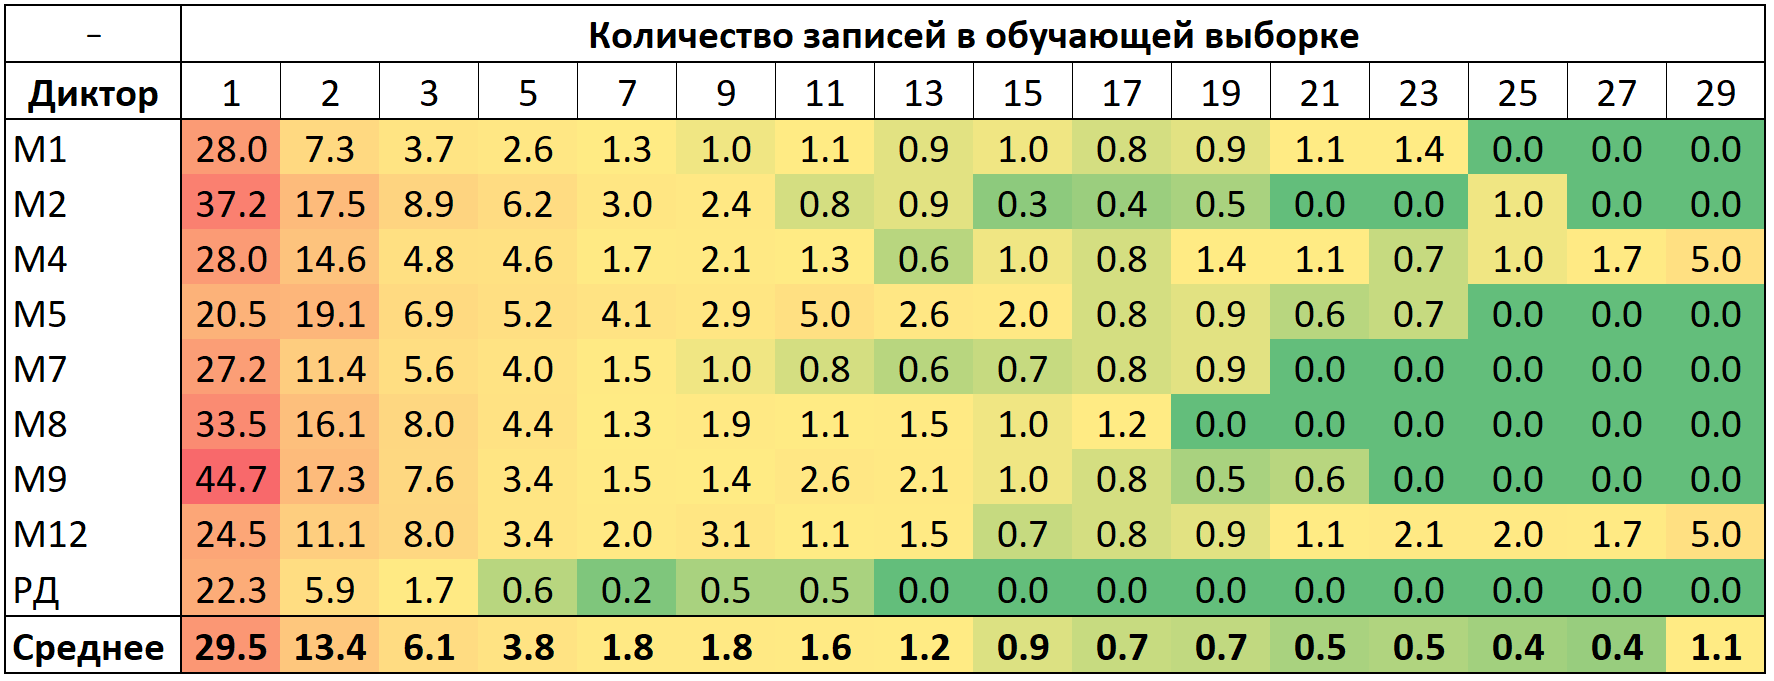
\includegraphics[width=1.0\textwidth]{cnn_words_self.png}
	\caption{Результаты распознавания слов свёрточной нейронной сетью при обучении на том же дикторе, в таблице указан процент неправильных распознаваний}
	\label{fig:cnn_words_self}
\end{figure}

Видно, что достаточно обучиться на 7 записях, чтобы ошибка стала ниже 2~\%, на 15 записях, чтобы стала ниже 1~\% и на 21 записи для 0.5~\% ошибок.
Данные результаты показывают, к каким величинам ошибок нужно стремиться при распознавании записей других дикторов для исключения эффекта дикторозависимости.

После этого проводилось распознавание с помощью одного диктора.
Это означает, что нейронная сеть обучалась на записях одного диктора и затем записи всех дикторов распознавались на этой нейронной сети.
При распознавании слов из обучающей выборки в среднем получается 0.0~\% ошибок, а для распознавания слов из тестовой выборки --- 5.9~\% ошибок.
Подробные результаты приведены в таблице \ref{tab:cnn_1dictor}.

\begin{table}[h]
	\centering
	\caption{Результаты распознавания слов свёрточной нейронной сетью на обучающем наборе из одного диктора в условиях без шума, в таблице указан процент неправильных распознаваний}
	\label{tab:cnn_1dictor}
	\begin{tabular}{| l | c | c | c | c | c | c | c | c | c |}
		\hline
		Набор & \multicolumn{9}{c|}{Диктор для распознавания} \\
		\hhline{~---------}
		обучения \phantom{00} & \phantom{0}М1\phantom{0} & \phantom{0}М2\phantom{0} & \phantom{0}М4\phantom{0} & \phantom{0}М5\phantom{0} & \phantom{0}М7\phantom{0} & \phantom{0}М8\phantom{0} & \phantom{0}М9\phantom{0} & \phantom{0}М12\phantom{0} & \phantom{0}РД\phantom{0} \\
		\hline
		М1		 & 0.0 & 6.3 & 2.5 & 7.7 &  7.8 &  8.2 &  2.5 &  4.7 & 5.3 \\
		М2		 & 1.7 & 0.0 & 0.7 & 3.3 &  2.7 &  9.5 &  6.0 &  8.3 & 1.0 \\
		М4		 & 2.7 & 6.2 & 0.2 & 3.0 &  3.0 &  5.3 &  5.0 &  6.8 & 0.8 \\
		М5		 & 6.2 & 7.8 & 2.0 & 0.0 &  7.3 &  6.0 &  6.5 &  2.8 & 3.3 \\
		М7		 & 9.5 & 7.8 & 2.3 & 5.5 &  0.0 & 22.0 & 10.3 & 24.5 & 3.7 \\
		М8		 & 4.5 & 4.7 & 2.8 & 3.3 & 10.0 &  0.0 &  6.3 &  2.5 & 3.0 \\
		М9		 & 2.3 & 6.7 & 3.7 & 3.7 &  7.5 &  7.8 &  0.0 &  7.5 & 2.7 \\
		М12		 & 5.2 & 7.3 & 6.0 & 4.7 &  9.2 &  6.3 &  8.0 &  0.0 & 3.8 \\
		РД		 & 7.2 & 7.7 & 4.0 & 4.7 &  2.5 &  9.3 & 11.3 & 13.2 & 0.0 \\
		\hline
	\end{tabular}
\end{table}

Далее было проведено распознавание с помощью трёх дикторов.
При распознавании слов из обучающей выборки в среднем получается 0.0~\% ошибок, а для распознавания слов из тестовой выборки --- 1.7~\% ошибок.
Подробные результаты приведены в таблице \ref{tab:cnn_3dictor}.

\begin{table}[h]
	\centering
	\caption{Результаты распознавания слов свёрточной нейронной сетью на обучающем наборе из трёх дикторов в условиях без шума, в таблице указан процент неправильных распознаваний}
	\label{tab:cnn_3dictor}
	\begin{tabular}{| l | c | c | c | c | c | c | c | c | c |}
		\hline
		Набор & \multicolumn{9}{c|}{Диктор для распознавания} \\
		\hhline{~---------}
		обучения  & \phantom{0}М1\phantom{0} & \phantom{0}М2\phantom{0} & \phantom{0}М4\phantom{0} & \phantom{0}М5\phantom{0} & \phantom{0}М7\phantom{0} & \phantom{0}М8\phantom{0} & \phantom{0}М9\phantom{0} & \phantom{0}М12\phantom{0} & \phantom{0}РД\phantom{0} \\
		\hline
		М1,М2,М4  & 0.0 & 0.0 & 0.2 & 2.3 & 0.7 & 3.7 & 2.0 & 2.7 & 0.7 \\
		М2,М4,М5  & 1.7 & 0.0 & 0.2 & 0.0 & 1.3 & 3.2 & 1.7 & 1.7 & 0.2 \\
		М4,М5,М7  & 2.3 & 2.2 & 0.2 & 0.0 & 0.0 & 3.3 & 1.7 & 4.0 & 0.3 \\
		М5,М7,М8  & 2.0 & 2.3 & 0.7 & 0.0 & 0.0 & 0.0 & 1.8 & 1.3 & 0.7 \\
		М7,М8,М9  & 1.3 & 1.7 & 0.7 & 1.0 & 0.0 & 0.0 & 0.0 & 1.8 & 0.0 \\
		М8,М9,М12 & 1.7 & 3.3 & 0.8 & 0.5 & 2.7 & 0.0 & 0.0 & 0.0 & 1.0 \\
		М9,М12,РД & 1.7 & 3.8 & 0.5 & 1.3 & 1.2 & 2.5 & 0.0 & 0.0 & 0.0 \\
		М12,РД,М1 & 0.0 & 2.3 & 0.5 & 1.2 & 2.0 & 1.7 & 1.8 & 0.0 & 0.0 \\
		РД,М1,М2  & 0.0 & 0.0 & 0.3 & 1.5 & 0.7 & 3.0 & 2.0 & 2.2 & 0.0 \\
		\hline
	\end{tabular}
\end{table}

Для распознавания большим числом дикторов были составлены несколько наборов данных для обучения.
Каждый набор состоит из записей слов 7 различных дикторов.
Далее на нейронных сетях, обученных на составленных наборах, производились распознавания на обучающей и тестовой выборках.
В таблице \ref{tab:cnn_without_noise} приведены результаты описанных распознаваний.

\begin{table}[h]
	\centering
	\caption{Результаты распознавания слов для случая записей без шума при распознавании на обучающем наборе из семи дикторов, в таблице указан процент неправильных распознаваний}
	\label{tab:cnn_without_noise}
	\begin{tabular}{| l | c | c | c | c | c | c | c | c | c |}
		\hline
		 & \multicolumn{9}{c|}{Диктор для распознавания} \\
		\hhline{----------}
		Набор обучения \phantom{0000000000000} & М1  & М2  & М4  & М5  & М7  & М8  & М9  & М12 & РД \\
		\hline
		М1,М2,М4,М5,М7,М8,М9  & 0.0 & 0.0 & 0.2 & 0.0 & 0.0 & 0.0 & 0.0 & 0.5 & 0.0 \\
		М2,М4,М5,М7,М8,М9,М12 & 0.8 & 0.0 & 0.2 & 0.0 & 0.0 & 0.0 & 0.0 & 0.0 & 0.0 \\
		М4,М5,М7,М8,М9,М12,РД & 1.2 & 1.2 & 0.2 & 0.0 & 0.0 & 0.0 & 0.0 & 0.0 & 0.0 \\
		М5,М7,М8,М9,М12,РД,М1 & 0.0 & 1.2 & 0.2 & 0.0 & 0.0 & 0.0 & 0.0 & 0.0 & 0.0 \\
		М7,М8,М9,М12,РД,М1,М2 & 0.0 & 0.0 & 0.5 & 0.5 & 0.0 & 0.0 & 0.0 & 0.0 & 0.0 \\
		М8,М9,М12,РД,М1,М2,М4 & 0.0 & 0.0 & 0.2 & 0.3 & 0.3 & 0.0 & 0.0 & 0.0 & 0.0 \\
		М9,М12,РД,М1,М2,М4,М5 & 0.0 & 0.0 & 0.2 & 0.0 & 0.7 & 1.2 & 0.0 & 0.0 & 0.0 \\
		М12,РД,М1,М2,М4,М5,М7 & 0.0 & 0.0 & 0.2 & 0.0 & 0.0 & 1.5 & 0.5 & 0.0 & 0.0 \\
		РД,М1,М2,М4,М5,М7,М8  & 0.0 & 0.0 & 0.2 & 0.0 & 0.0 & 0.0 & 0.7 & 0.5 & 0.0 \\
		\hline
	\end{tabular}
\end{table}

При распознавании слов из обучающей выборки ошибок нет, а для распознавания слов из тестовой выборки в среднем получается 0.6~\% ошибок.

В таблице \ref{tab:cnn_without_noise_summary} приведены суммарные результаты распознавания записей без шума при обучении на различном числе дикторов.

\begin{table}[h]
	\centering
	\caption{Суммарные результаты распознаваний слов на обучающих наборах из различного количества дикторов для случая записей без шума}
	\label{tab:cnn_without_noise_summary}
	\begin{tabular}{| l | c | c | c | c | c | c | c |}
		\hline
		Количество дикторов	\phantom{000} & \phantom{00}1\phantom{00} & \phantom{00}2\phantom{00} & \phantom{00}3\phantom{00} & \phantom{00}4\phantom{00} & \phantom{00}5\phantom{00} & \phantom{00}6\phantom{00} & \phantom{00}7\phantom{00} \\
		\hline
		Процент ошибок		& 5.9 & 2.4 & 1.7 & 1.2 & 1.0 & 0.8 & 0.6 \\
		\hline
	\end{tabular}
\end{table}

Из результатов можно сделать вывод, что процент ошибок стабильно снижается при увеличении количества дикторов в обучающей базе.
Большее число дикторов позволяет избавиться от дикторозависимости, что положительно сказывается на качестве распознавания.

\clearpage

%\newpage
%============================================================================================================================

\section{Обучение и тестирование свёрточной нейронной сети глубокого обучения на данных содержащих шум кабины пилотов современного магистрального самолёта} \label{sect4_4}

В данном подразделе приведены результаты распознавания записей в условиях шума.
Шум моделировался следующим образом.
Для каждой записи выбирались уникальные отрезки шума из записи шума кабины самолёта Boeing со средней громкостью более 80 дБ.
При этом громкость шума нормировалась так, чтобы отношение сигнал/шум было равно некоторой фиксированной величине.

Проведён эксперимент по распознаванию записей того же диктора, записи которого использовались в качестве обучающей выборки.
Также как и случае записей без шума, записи каждого диктора разбивались на 2 части: на первой части обучалась свёрточная нейронная сеть, а вторая часть использовалась в качестве тестовой выборки.
Результаты этих распознаваний приведены на рисунке \ref{fig:cnn_words_self_noise}.
По столбцам отложено количество записей для каждого слова, содержащихся в обучающей выборке.
В столбцах указан уровень наложенного шума.
Приведённые результаты являются усреднёнными значениями по всем дикторам.

\begin{figure}[h]
	\centering
	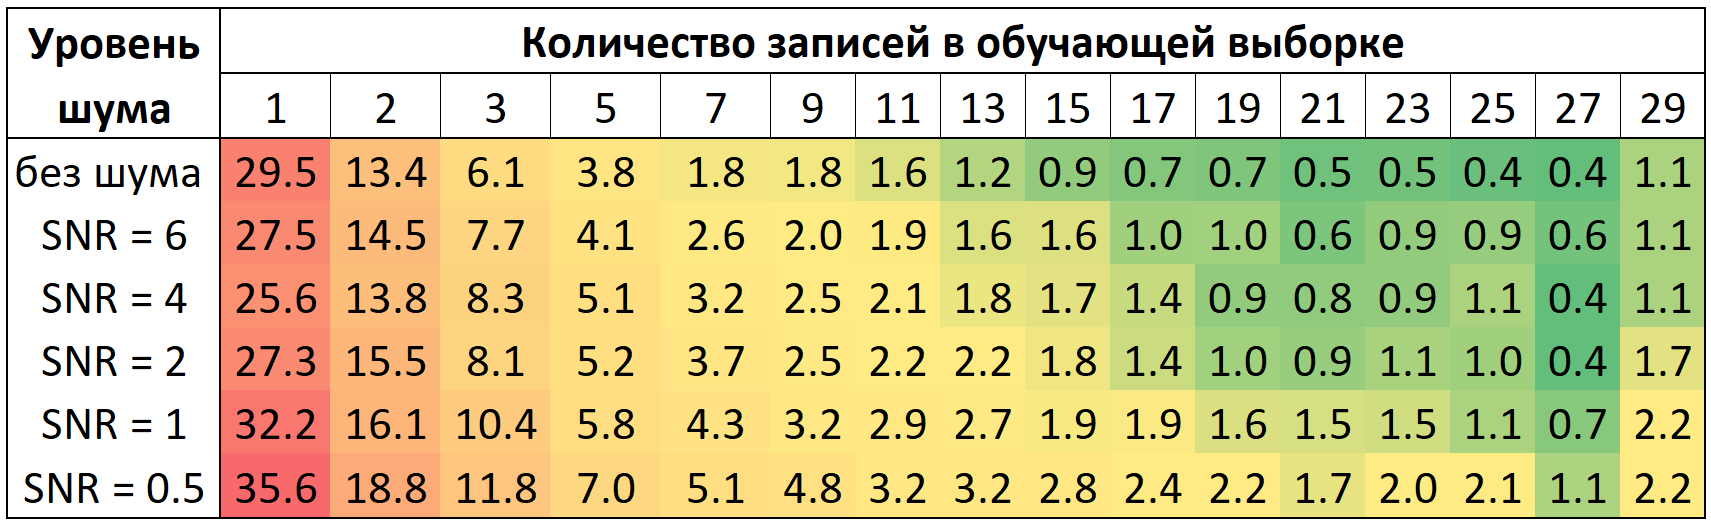
\includegraphics[width=1.0\textwidth]{cnn_words_self_noise.png}
	\caption{Усреднённые результаты распознавания слов свёрточной нейронной сетью в условиях различных уровней шума при обучении на том же дикторе, в таблице указан процент неправильных распознаваний}
	\label{fig:cnn_words_self_noise}
\end{figure}

Видно, что результаты монотонно ухудшаются с увеличением уровня шума, при этом по величине ухудшение оказывается незначительным.
Например, при использовании 15 записей в обучающей выборке при отсутствии шума получается 0.9~\% ошибок, а при отношении сигнал/шум равном 1 получается 1.9~\% ошибок.
Аналогичные значения при обучении на 9 записях равны 1.8 и 3.2~\% соответственно.
Данные результаты показывают, к каким величинам ошибок нужно стремиться при распознавании записей с шумом других дикторов для исключения эффекта дикторозависимости.

После этого было проведено обычное распознавание одним диктором с наложением одного варианта шума.
Здесь и далее громкость шума нормировалась так, чтобы отношение сигнал/шум было равно 4.
Для увеличения обучающей выборки и улучшения процесса обучения на записи могут накладываться различные уникальные варианты шума.
В таблице \ref{tab:cnn_1noise_1dictor} представлено 2 варианта эксперимента.
В первом случае обучение проводилось на записях с шумом, а распознавались записи без шума.

\begin{table}[h]
	\centering
	\caption{Результаты распознавания слов для случая записей с шумом при распознавании на обучающем наборе из одного диктора, в таблице указан процент неправильных распознаваний}
	\label{tab:cnn_1noise_1dictor}
	\begin{tabular}{| l | c | c | c | c | c | c | c | c | c |}
		\hline
		Набор & \multicolumn{9}{c|}{Диктор для распознавания} \\
		\hhline{~---------}
		обучения\phantom{00} & \phantom{0}М1\phantom{0} & \phantom{0}М2\phantom{0} & \phantom{0}М4\phantom{0} & \phantom{0}М5\phantom{0} & \phantom{0}М7\phantom{0} & \phantom{0}М8\phantom{0} & \phantom{0}М9\phantom{0} & \phantom{0}М12\phantom{0} & \phantom{0}РД\phantom{0} \\
		\hline
		\multicolumn{10}{|c|}{обучение с шумом, распознавание без шума} \\
		\hline
		М1		 &  0.0 & 13.8 &  6.3 & 12.2 & 11.7 & 14.8 &  9.3 & 16.7 &  9.0 \\
		М2		 &  7.2 &  0.2 & 15.8 & 12.0 & 27.7 & 10.0 & 18.3 &  9.2 & 11.5 \\
		М4		 &  5.8 &  7.0 &  0.3 & 10.0 &  6.5 & 10.3 &  7.3 & 13.2 &  1.3 \\
		М5		 &  7.0 & 10.0 &  3.8 &  0.0 & 13.0 &  7.5 & 11.8 &  4.8 &  8.0 \\
		М7		 & 14.5 & 13.3 &  7.3 & 15.2 &  0.2 & 18.2 & 14.7 & 24.7 &  5.3 \\
		М8		 &  9.2 &  7.8 &  7.7 &  7.5 & 16.3 &  0.0 & 12.2 &  8.7 &  5.2 \\
		М9		 &  5.0 & 11.2 &  8.5 &  9.2 & 14.2 & 11.3 &  0.0 & 14.3 & 10.3 \\
		М12		 & 12.3 & 11.0 & 16.3 & 14.8 & 16.8 & 14.3 & 18.5 &  0.2 &  9.3 \\
		РД		 & 19.7 & 14.8 & 11.5 & 15.2 &  8.7 & 19.5 & 18.7 & 24.2 &  1.7 \\
		\hline
		\multicolumn{10}{|c|}{обучение с шумом, распознавание с шумом} \\
		\hline
		М1		 &  0.0 & 11.2 &  5.7 & 14.0 & 14.2 & 17.0 &  4.3 & 11.8 &  8.3 \\
		М2		 &  3.3 &  0.0 &  2.2 &  5.0 &  8.3 & 11.5 &  7.2 &  8.2 &  1.2 \\
		М4		 &  5.3 & 10.2 &  0.0 & 11.3 &  5.3 & 16.3 &  7.5 & 12.0 &  2.3 \\
		М5		 &  8.0 & 10.2 &  3.3 &  0.0 & 11.5 & 10.2 &  8.5 &  4.7 &  8.2 \\
		М7		 & 11.7 & 12.2 &  5.3 & 11.8 &  0.0 & 26.8 & 12.3 & 25.7 &  0.8 \\
		М8		 &  7.8 &  8.5 &  5.7 &  4.7 & 10.0 &  0.0 & 11.7 &  8.8 &  6.0 \\
		М9		 &  5.3 &  9.3 &  8.2 &  9.2 & 10.3 & 20.2 &  0.0 & 19.5 & 13.2 \\
		М12		 &  8.8 & 11.2 &  7.7 &  8.0 &  8.7 & 14.5 & 10.0 &  0.0 &  6.2 \\
		РД		 & 10.5 & 11.2 &  5.8 & 11.2 &  4.5 & 14.8 & 15.2 & 19.7 &  0.0 \\
		\hline
	\end{tabular}
\end{table}

Средняя ошибка при распознавании записей диктора, на которых проводилось обучение, равна 0.3~\%, а средняя ошибка для записей других дикторов --- 11.8~\%.
Во втором случае и обучение, и распознавание проводилось на записях с шумом.
На записях, на которых проводилось обучение, ошибок не было, а средняя ошибка для записей других дикторов равна 9.7~\%.
Из этих результатов видно, что для обоих вариантов распознавания ошибка получается выше, чем при использовании записей без шума.
Также проводился эксперимент, в котором обучение проводилось на записях без шума, а распознавания на записях с шумом.
Для этого варианта количество ошибок получалось в несколько раз больше, чем для предыдущих, поэтому в дальнейшем такой вариант использоваться не будет.

Далее был проведён аналогичный эксперимент, но с тем отличием, что для обучения использовались записи с семью различными наложенными вариантами шума.
Для первого эксперимента средняя ошибка при распознавании записей диктора, на которых проводилось обучение, равна 0.0~\%, а средняя ошибка для записей других дикторов --- 8.5~\%.
Для второго эксперимента на записях, на которых проводилось обучение, ошибок не было, а средняя ошибка для записей других дикторов равна 8.2~\%.
Как видно из результатов, использование нескольких вариантов шумов заметно улучшает качество распознавания.
Результаты данных экспериментов приведены в таблице \ref{tab:cnn_7noise_1dictor}.

\begin{table}[h]
	\centering
	\caption{Результаты распознавания слов для случая записей с шумом при распознавании на обучающем наборе из одного диктора с 7 вариантами шума, в таблице указан процент неправильных распознаваний}
	\label{tab:cnn_7noise_1dictor}
	\begin{tabular}{| l | c | c | c | c | c | c | c | c | c |}
		\hline
		Набор & \multicolumn{9}{c|}{Диктор для распознавания} \\
		\hhline{~---------}
		обучения\phantom{00} & \phantom{0}М1\phantom{0} & \phantom{0}М2\phantom{0} & \phantom{0}М4\phantom{0} & \phantom{0}М5\phantom{0} & \phantom{0}М7\phantom{0} & \phantom{0}М8\phantom{0} & \phantom{0}М9\phantom{0} & \phantom{0}М12\phantom{0} & \phantom{0}РД\phantom{0} \\
		\hline
		\multicolumn{10}{|c|}{обучение с шумом, распознавание без шума} \\
		\hline
		М1		 &  0.0 & 10.2 &  5.8 & 10.8 & 10.3 & 13.5 &  7.3 & 11.7 & 10.3 \\
		М2		 &  3.7 &  0.0 &  2.5 &  5.0 &  9.2 &  9.5 &  7.8 &  5.2 &  1.2 \\
		М4		 &  4.5 &  7.3 &  0.2 &  6.3 &  5.8 &  8.5 &  8.7 &  9.8 &  2.3 \\
		М5		 &  6.0 &  8.3 &  2.2 &  0.0 &  7.0 &  4.7 &  7.0 &  4.2 &  5.7 \\
		М7		 & 12.2 & 12.3 &  6.0 & 15.5 &  0.0 & 21.2 &  9.3 & 29.0 &  4.3 \\
		М8		 &  6.0 &  5.7 &  3.7 &  3.3 &  7.8 &  0.0 &  9.2 &  8.8 &  4.2 \\
		М9		 &  4.7 & 10.5 &  7.3 &  7.3 & 12.0 &  7.5 &  0.0 & 10.0 & 11.7 \\
		М12		 &  8.7 &  9.8 & 10.8 & 11.0 &  9.2 & 10.0 &  7.5 &  0.0 &  5.2 \\
		РД		 & 13.3 & 10.8 &  5.7 &  8.2 &  4.3 & 12.3 & 15.2 & 19.3 &  0.0 \\
		\hline
		\multicolumn{10}{|c|}{обучение с шумом, распознавание с шумом} \\
		\hline
		М1		 &  0.0 &  8.5 &  4.0 &  9.5 & 13.7 & 13.3 &  3.8 &  8.3 &  7.2 \\
		М2		 &  2.5 &  0.0 &  2.7 &  5.5 &  5.8 & 12.5 &  5.8 &  5.0 &  1.7 \\
		М4		 &  6.0 &  7.3 &  0.0 &  9.5 &  5.2 & 13.3 &  8.3 & 11.3 &  2.0 \\
		М5		 &  5.7 &  8.2 &  1.5 &  0.0 &  7.8 &  7.8 &  7.3 &  4.7 &  4.8 \\
		М7		 & 10.7 & 12.2 &  5.7 & 13.2 &  0.0 & 24.2 & 10.7 & 20.5 &  1.3 \\
		М8		 &  5.0 &  8.2 &  3.3 &  4.2 &  8.2 &  0.0 &  8.7 & 10.7 &  3.8 \\
		М9		 &  4.3 & 10.5 &  5.7 &  6.7 &  7.2 & 15.7 &  0.0 & 13.0 &  6.8 \\
		М12		 &  7.8 & 11.5 &  7.0 &  6.5 &  7.3 & 12.5 &  5.3 &  0.0 &  5.8 \\
		РД		 & 10.8 & 13.5 &  5.3 & 10.5 &  3.5 & 15.5 & 14.3 & 13.5 &  0.0 \\
		\hline
	\end{tabular}
\end{table}

После этого было проведено обучение нейронной сети на 3 дикторах в условиях шума и последующее распознавания записей.
Первый эксперимент предполагает использование одного варианта шума при обучении, а второй эксперимент --- 3 варианта шума.
В обоих случаях средняя величина ошибки при распознавании записей диктора, на которых проводилось обучение, равна 0.0~\%.
Для случая распознавания записей других дикторов ошибка равна 2.8~\% для первого эксперимента и 2.5~\% для второго.
Подробные результаты экспериментов приведены в таблице \ref{tab:cnn_noise_3dictors}.

\begin{table}[h]
	\centering
	\caption{Результаты распознавания слов для случая записей с шумом при распознавании на обучающем наборе из трёх дикторов с 1 и 3 вариантами шума, в таблице указан процент неправильных распознаваний}
	\label{tab:cnn_noise_3dictors}
	\begin{tabular}{| l | c | c | c | c | c | c | c | c | c |}
		\hline
		Набор & \multicolumn{9}{c|}{Диктор для распознавания} \\
		\hhline{~---------}
		обучения  & \phantom{0}М1\phantom{0} & \phantom{0}М2\phantom{0} & \phantom{0}М4\phantom{0} & \phantom{0}М5\phantom{0} & \phantom{0}М7\phantom{0} & \phantom{0}М8\phantom{0} & \phantom{0}М9\phantom{0} & \phantom{0}М12\phantom{0} & \phantom{0}РД\phantom{0} \\
		\hline
		\multicolumn{10}{|c|}{1 вариант шума} \\
		\hline
		М1,М2,М4  & 0.0 & 0.0 & 0.2 & 4.0 & 2.7 & 7.3 & 3.5 & 2.7 & 0.8 \\
		М2,М4,М5  & 2.5 & 0.0 & 0.2 & 0.0 & 2.7 & 4.5 & 3.8 & 1.3 & 0.5 \\
		М4,М5,М7  & 3.5 & 4.3 & 0.2 & 0.0 & 0.0 & 5.7 & 3.8 & 4.0 & 0.3 \\
		М5,М7,М8  & 2.8 & 3.5 & 1.2 & 0.0 & 0.0 & 0.0 & 4.2 & 2.0 & 0.5 \\
		М7,М8,М9  & 2.7 & 3.7 & 1.2 & 1.0 & 0.0 & 0.0 & 0.0 & 2.0 & 0.2 \\
		М8,М9,М12 & 2.3 & 4.3 & 1.5 & 1.0 & 3.5 & 0.0 & 0.0 & 0.0 & 3.5 \\
		М9,М12,РД & 2.3 & 4.3 & 1.0 & 2.3 & 2.8 & 6.5 & 0.0 & 0.0 & 0.0 \\
		М12,РД,М1 & 0.0 & 4.7 & 1.2 & 2.3 & 2.8 & 6.5 & 2.2 & 0.0 & 0.0 \\
		РД,М1,М2  & 0.0 & 0.0 & 1.5 & 0.8 & 1.8 & 6.7 & 2.5 & 1.8 & 0.0 \\
		\hline
		\multicolumn{10}{|c|}{3 варианта шума} \\
		\hline
		М1,М2,М4  & 0.0 & 0.0 & 0.2 & 2.0 & 2.8 & 7.3 & 2.8 & 2.3 & 1.7 \\
		М2,М4,М5  & 0.8 & 0.0 & 0.2 & 0.0 & 2.3 & 3.7 & 2.7 & 2.2 & 1.3 \\
		М4,М5,М7  & 2.5 & 4.2 & 0.2 & 0.0 & 0.0 & 5.0 & 3.7 & 2.0 & 0.5 \\
		М5,М7,М8  & 2.3 & 3.0 & 1.2 & 0.0 & 0.0 & 0.0 & 3.2 & 2.0 & 0.7 \\
		М7,М8,М9  & 2.5 & 3.5 & 1.0 & 0.5 & 0.0 & 0.0 & 0.0 & 2.5 & 0.2 \\
		М8,М9,М12 & 3.3 & 4.5 & 2.3 & 0.7 & 3.3 & 0.0 & 0.0 & 0.0 & 2.7 \\
		М9,М12,РД & 2.8 & 4.7 & 1.0 & 1.2 & 2.7 & 5.7 & 0.0 & 0.0 & 0.0 \\
		М12,РД,М1 & 0.0 & 2.3 & 1.5 & 1.7 & 2.3 & 4.8 & 1.8 & 0.0 & 0.0 \\
		РД,М1,М2  & 0.0 & 0.0 & 0.7 & 1.7 & 1.8 & 8.2 & 1.8 & 1.8 & 0.0 \\
		\hline
	\end{tabular}
\end{table}

Из полученных в данном и предыдущих экспериментах результатов можно сделать вывод, что использование дополнительных вариантов шума, наложенных на одни и те же исходные записи помогает улучшить обучение нейронной сети и, как следствие, качество распознавания речевых команд.
То есть практика показывает, что чем больше вариантов шума используется, тем лучше получаются результаты.
Единственное ограничение --- это вычислительная мощность компьютера, используемого при обучении нейронной сети.

Результаты эксперимента на записях с наложенным шумом при обучении на 7 дикторах приведены в таблице \ref{tab:cnn_3noise_7dictors}.

\begin{table}[h]
	\centering
	\caption{Результаты распознавания слов для случая записей с шумом при распознавании на обучающем наборе из семи дикторов с 1 и 3 вариантами шума, в таблице указан процент неправильных распознаваний}
	\label{tab:cnn_3noise_7dictors}
	\begin{tabular}{| l | c | c | c | c | c | c | c | c | c |}
		\hline
		Набор & \multicolumn{9}{c|}{Диктор для распознавания} \\
		\hhline{~---------}
		обучения \phantom{0000000000000000000} & М1  & М2  & М4  & М5  & М7  & М8  & М9  & М12 & РД \\
		\hline
		\multicolumn{10}{|c|}{1 вариант шума} \\
		\hline
		М1,М2,М4,М5,М7,М8,М9  & 0.0 & 0.0 & 0.2 & 0.0 & 0.0 & 0.0 & 0.0 & 1.3 & 0.3 \\
		М2,М4,М5,М7,М8,М9,М12 & 1.3 & 0.0 & 0.2 & 0.0 & 0.0 & 0.0 & 0.0 & 0.0 & 0.2 \\
		М4,М5,М7,М8,М9,М12,РД & 1.3 & 2.0 & 0.2 & 0.0 & 0.0 & 0.0 & 0.0 & 0.0 & 0.0 \\
		М5,М7,М8,М9,М12,РД,М1 & 0.0 & 1.8 & 0.3 & 0.0 & 0.0 & 0.0 & 0.0 & 0.0 & 0.0 \\
		М7,М8,М9,М12,РД,М1,М2 & 0.0 & 0.0 & 0.5 & 0.2 & 0.0 & 0.0 & 0.0 & 0.0 & 0.0 \\
		М8,М9,М12,РД,М1,М2,М4 & 0.0 & 0.0 & 0.2 & 0.2 & 1.3 & 0.0 & 0.0 & 0.0 & 0.0 \\
		М9,М12,РД,М1,М2,М4,М5 & 0.0 & 0.0 & 0.2 & 0.0 & 1.0 & 3.0 & 0.0 & 0.0 & 0.0 \\
		М12,РД,М1,М2,М4,М5,М7 & 0.0 & 0.0 & 0.2 & 0.0 & 0.0 & 2.3 & 1.5 & 0.0 & 0.0 \\
		РД,М1,М2,М4,М5,М7,М8  & 0.0 & 0.0 & 0.2 & 0.0 & 0.0 & 0.0 & 1.7 & 0.7 & 0.0 \\	
		\hline
		\multicolumn{10}{|c|}{3 варианта шума} \\
		\hline
		М1,М2,М4,М5,М7,М8,М9  & 0.0 & 0.0 & 0.2 & 0.0 & 0.0 & 0.0 & 0.0 & 0.8 & 0.3 \\
		М2,М4,М5,М7,М8,М9,М12 & 1.0 & 0.0 & 0.2 & 0.0 & 0.0 & 0.0 & 0.0 & 0.0 & 0.2 \\
		М4,М5,М7,М8,М9,М12,РД & 1.7 & 2.0 & 0.2 & 0.0 & 0.0 & 0.0 & 0.0 & 0.0 & 0.0 \\
		М5,М7,М8,М9,М12,РД,М1 & 0.0 & 1.2 & 0.2 & 0.0 & 0.0 & 0.0 & 0.0 & 0.0 & 0.0 \\
		М7,М8,М9,М12,РД,М1,М2 & 0.0 & 0.0 & 0.2 & 0.3 & 0.0 & 0.0 & 0.0 & 0.0 & 0.0 \\
		М8,М9,М12,РД,М1,М2,М4 & 0.0 & 0.0 & 0.2 & 0.2 & 1.5 & 0.0 & 0.0 & 0.0 & 0.0 \\
		М9,М12,РД,М1,М2,М4,М5 & 0.0 & 0.0 & 0.2 & 0.0 & 1.2 & 3.0 & 0.0 & 0.0 & 0.0 \\
		М12,РД,М1,М2,М4,М5,М7 & 0.0 & 0.0 & 0.2 & 0.0 & 0.0 & 2.2 & 1.5 & 0.0 & 0.0 \\
		РД,М1,М2,М4,М5,М7,М8  & 0.0 & 0.0 & 0.2 & 0.0 & 0.0 & 0.0 & 1.5 & 0.7 & 0.0 \\
		\hline
	\end{tabular}
\end{table}

В данном эксперименте при обучении использовалось 3 варианта шума.
При распознавании слов из обучающей выборки средняя ошибка равна 0.0~\%, а для распознавания слов из тестовой выборки получается в среднем 1.1~\% ошибок.

В таблице \ref{tab:cnn_with_noise_summary} приведены суммарные результаты распознавания записей с шумом при обучении на различном числе дикторов и различном количестве наложенных шумов.

\begin{table}[h]
	\centering
	\caption{Суммарные результаты распознавания на обучающей выборке и на тестовой выборке при обучении на различном числе дикторов для случаев записей слов без шума и с шумом, в таблице указан процент неправильных распознаваний}
	\label{tab:cnn_with_noise_summary}
	\begin{tabular}{| l | c | c | c | c |}
		\hline
		Число				& \phantom{0}Наличие\phantom{0} & \phantom{0} Число \phantom{0} 	& \multicolumn{2}{c|}{Процент ошибок}	\\
		\hhline{~~~--}
		дикторов			& шума  			& шумов 	& обучающая выборка & тестовая выборка	\\
		\hline
		\multirow{4}{*}{1 диктор}	& \multirow{2}{*}{без шума}	& 1				& 0.3 		& 11.8 		\\
		\hhline{~~---}
		&    						& 7				& 0.0 		& 8.5  		\\
		\hhline{~----}
		& \multirow{2}{*}{с шумом}	& 1				& 0.3 		& 9.7  		\\
		\hhline{~~---}
		&    						& 7				& 0.0 		& 8.2  		\\
		\hline
		\multirow{2}{*}{3 диктора}	& \multirow{2}{*}{с шумом}	& 1				& 0.0 		& 2.8  		\\
		\hhline{~~---}
		&    						& 3				& 0.0 		& 2.5  		\\
		\hline
		\multirow{2}{*}{7 дикторов}	& \multirow{2}{*}{с шумом}	& 1				& 0.0 		& 1.2  		\\
		\hhline{~~---}
		&    						& 3				& 0.0 		& 1.1  		\\
		\hline
	\end{tabular}
\end{table}

Из результатов можно сделать вывод, аналогичный выводу в предыдущем подразделе, что процент ошибок стабильно снижается по тем же причинам при увеличении количества дикторов в обучающей базе.
Также можно сделать вывод, что увеличение количества накладываемых шумов приводит к уменьшению числа ошибок, но этот эффект от увеличения обучающей базы выражен менее заметно.
Большое количество шумов в обучающей выборке уменьшает эффект переобучения для определённого типа шума, что уменьшает число ошибок при распознавании записей с другим шумом.
Другими словами, <<шумонезависимость>> аналогична дикторонезависимости и достигается путём увеличения количества разных шумов в обучающей выборке.

И результаты экспериментов с шумом, и результаты без шума оказалась самыми лучшими при использовании свёрточных нейронных сетей глубокого обучения.
К недостаткам этого алгоритма можно отнести большую вычислительную сложность обучения сети.
При этом, само распознавания происходит практически мгновенно.

\clearpage

%\newpage
%============================================================================================================================

\section{Исследование возможности применения свёрточной нейронной сети глубокого обучения для распознавания отдельных фраз} \label{sect4_5}

Для распознавания речевых команд в форме фраз использовалась такая же архитектура нейронных сетей, как и для слов, описанная в подразделе \ref{sect4_2}.
При этом, был произведён подбор параметров свёрточной нейронной сети, которые во многом оказались схожими с параметрами, найденными для распознавания слов.
Оптимальный размер пачки равен 330, т.е. в неё включены все записи фраз.
Оптимальное количество итераций --- 10000 и скорость обучения 0.0001.
Подробные результаты подбора приведены ниже в таблице \ref{tab:cnn_phrases_bf_iter_pace}.

\begin{table}[h]
	\centering
	\caption{Подбор количества итераций и скорости обучения для свёрточной нейронной сети при распознавании фраз, в таблице указан процент неправильных распознаваний}
	\label{tab:cnn_phrases_bf_iter_pace}
	\begin{tabular}{| l | c | c | c | c | c |}
		\hline
		Скорость & \multicolumn{5}{c|}{Количество итераций} \\
		\hhline{~-----}
		обучения \phantom{00} & \phantom{000} 100 \phantom{000} & \phantom{000}1000\phantom{000} & \phantom{000}3000\phantom{000} & \phantom{00} 10000 \phantom{00} & \phantom{00} 30000 \phantom{00} \\
		\hline
		0.00001	& 55.60 & 26.90 & 24.40 & 22.50 & 21.20 \\
		0.00003	& 36.50 & 24.30 & 22.40 & 22.30 & 20.40 \\
		0.0001	& 31.80 & 23.10 & 23.00 & \textbf{20.40} & 20.30 \\
		0.0003	& 61.40 & 41.30 & 39.20 & 22.20 & 21.30 \\
		0.001	& 90.90 & 22.60 & 23.40 & 22.80 & 30.00 \\
		0.003	& 90.90 & 75.40 & 45.40 & 44.90 & 63.20 \\
		0.01	& 90.90 & 90.90 & 90.90 & 90.90 & 90.90 \\
		\hline
	\end{tabular}
\end{table}

Вначале проводился эксперимент по распознаванию записей того же диктора, на котором происходило обучение нейронной сети.
Постановка задачи аналогична случаю распознавания слов и описана в начале подраздела \ref{sect4_3}.
Результаты этих распознаваний приведены на рисунке \ref{fig:cnn_phrases_self}.

\begin{figure}[h]
	\centering
	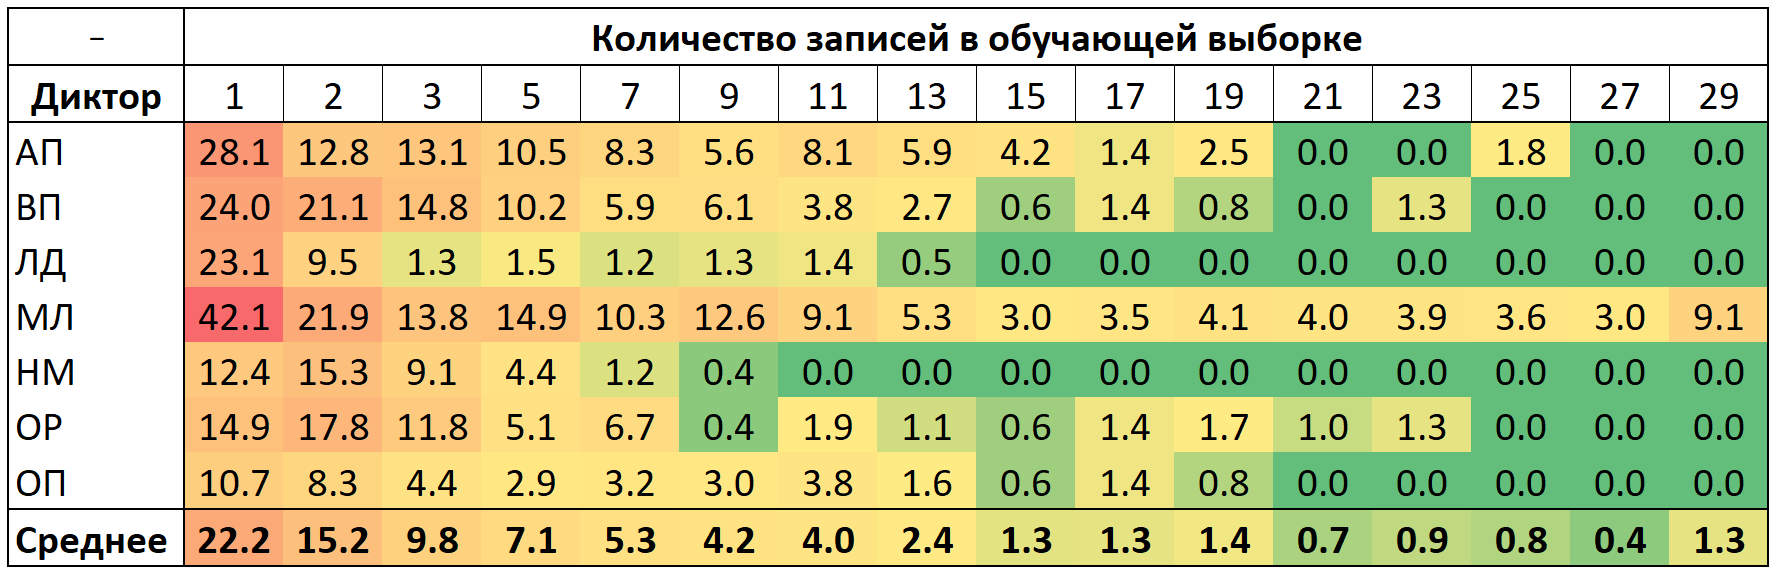
\includegraphics[width=1.0\textwidth]{cnn_phrases_self.png}
	\caption{Результаты распознавания фраз свёрточной нейронной сетью при обучении на других записях соответствующего диктора, в таблице указан процент неправильных распознаваний}
	\label{fig:cnn_phrases_self}
\end{figure}

Видно, что достаточно обучиться на 9 записях, чтобы ошибка стала ниже 5~\%, на 15 записях, чтобы стала ниже 2~\% и на 21 записи для 1~\% ошибок.

Аналогично распознаванию слов проводилось распознавание фраз при обучении нейронной сети на данных одного диктора в условиях без шума.
При распознавании слов из обучающей выборки в среднем получается 0.0~\% ошибок, а для распознавания слов из тестовой выборки --- 18.0~\% ошибок.
Подробные результаты приведены в таблице \ref{tab:cnn_phrases_1dictor}.

\begin{table}[h]
	\centering
	\caption{Результаты распознавания фраз свёрточной нейронной сетью на обучающем наборе из одного диктора в условиях без шума, в таблице указан процент неправильных распознаваний}
	\label{tab:cnn_phrases_1dictor}
	\begin{tabular}{| l | c | c | c | c | c | c | c |}
		\hline
		Набор & \multicolumn{7}{c|}{Диктор для распознавания} \\
		\hhline{~-------}
		обучения \phantom{0000} & \phantom{0} АП \phantom{0} & \phantom{0} ВП \phantom{0} & \phantom{0} ЛД \phantom{0} & \phantom{0} МЛ \phantom{0} & \phantom{0} НМ \phantom{0} & \phantom{0} ОР \phantom{0} & \phantom{0} ОП \phantom{0} \\
		\hline
		АП 		 &  0.0 & 31.2 & 61.2 & 20.3 & 36.4 & 43.6 & 13.9 \\
		ВП 		 & 21.5 &  0.0 & 12.1 & 21.5 &  3.0 &  9.4 &  9.7 \\
		ЛД 		 & 37.6 &  7.9 &  0.0 & 21.8 & 13.0 & 21.2 & 18.8 \\
		МЛ 		 & 10.0 & 10.3 & 13.3 &  0.0 &  5.5 & 15.5 &  2.1 \\
		НМ 		 & 30.0 &  6.4 & 11.2 & 22.1 &  0.0 & 18.2 &  7.3 \\
		ОР 		 & 41.2 &  9.4 & 18.2 & 24.8 &  9.4 &  0.0 & 10.3 \\
		ОП 		 & 16.1 & 10.3 & 23.0 & 11.2 &  9.7 & 17.9 &  0.0 \\
		\hline
	\end{tabular}
\end{table}

Далее было проведено распознавание фраз с помощью трёх дикторов.
При распознавании фраз из обучающей выборки в среднем получается 0.0~\% ошибок, а для распознавания слов из тестовой выборки --- 6.9~\% ошибок.
Подробные результаты приведены в таблице \ref{tab:cnn_phrases_3dictors}.

\begin{table}[h]
	\centering
	\caption{Результаты распознавания фраз свёрточной нейронной сетью на обучающем наборе из трёх дикторов в условиях без шума, в таблице указан процент неправильных распознаваний}
	\label{tab:cnn_phrases_3dictors}
	\begin{tabular}{| l | c | c | c | c | c | c | c |}
		\hline
		Набор & \multicolumn{7}{c|}{Диктор для распознавания} \\
		\hhline{~-------}
		обучения \phantom{0000} & \phantom{0} АП \phantom{0} & \phantom{0} ВП \phantom{0} & \phantom{0} ЛД \phantom{0} & \phantom{0} МЛ \phantom{0} & \phantom{0} НМ \phantom{0} & \phantom{0} ОР \phantom{0} & \phantom{0} ОП \phantom{0} \\
		\hline
		АП,ВП,ЛД &  0.0 &  0.0 &  0.0 &  5.2 &  1.5 & 12.4 &  2.7 \\
		ВП,ЛД,МЛ & 10.0 &  0.0 &  0.0 &  0.0 &  2.4 &  7.9 &  1.2 \\
		ЛД,МЛ,НМ & 12.7 &  5.8 &  0.0 &  0.0 &  0.0 &  8.8 &  3.0 \\
		МЛ,НМ,ОР & 13.6 &  5.8 &  5.5 &  0.0 &  0.0 &  0.0 &  1.5 \\
		НМ,ОР,ОП & 26.4 &  4.8 &  7.0 & 11.8 &  0.0 &  0.0 &  0.0 \\
		ОР,ОП,АП &  0.0 &  3.6 &  9.7 &  6.1 &  4.2 &  0.0 &  0.0 \\
		ОП,АП,ВП &  0.0 &  0.0 &  3.6 &  5.8 &  3.0 &  6.1 &  0.0 \\
		\hline
	\end{tabular}
\end{table}

Для распознавания несколькими дикторами были составлены несколько наборов данных для обучения.
Каждый набор состоит из записей фраз 6 различных дикторов.
Далее на нейронных сетях, обученных на приведённых наборах, производились распознавания на обучающей и тестовой выборках.
Как видно из таблицы \ref{tab:cnn_phrases_6dictors}, для случая фраз без шума средний результат лучше, чем при распознавании одним или тремя дикторами.

\begin{table}[h]
	\centering
	\caption{Результаты распознавания фраз свёрточной нейронной сетью на обучающем наборе из шести дикторов в условиях без шума, в таблице указан процент неправильных распознаваний}
	\label{tab:cnn_phrases_6dictors}
	\begin{tabular}{| l | c | c | c | c | c | c | c |}
		\hline
		Набор & \multicolumn{7}{c|}{Диктор для распознавания} \\
		\hhline{~-------}
		обучения & \phantom{0}АП\phantom{0} & \phantom{0}ВП\phantom{0} & \phantom{0}ЛД\phantom{0} & \phantom{0}МЛ\phantom{0} & \phantom{0}НМ\phantom{0} & \phantom{0}ОР\phantom{0} & \phantom{0}ОП\phantom{0} \\
		\hline
		АП,ВП,ЛД,МЛ,НМ,ОР	 &  0.0 &  0.0 &  0.0 &  0.0 &  0.0 &  0.0 &  1.5 \\
		ВП,ЛД,МЛ,НМ,ОР,ОП	 & 10.0 &  0.0 &  0.0 &  0.0 &  0.0 &  0.0 &  0.0 \\
		ЛД,МЛ,НМ,ОР,ОП,АП	 &  0.0 &  2.4 &  0.0 &  0.0 &  0.0 &  0.0 &  0.0 \\
		МЛ,НМ,ОР,ОП,АП,ВП	 &  0.0 &  0.0 &  3.3 &  0.0 &  0.0 &  0.0 &  0.0 \\
		НМ,ОР,ОП,АП,ВП,ЛД	 &  0.0 &  0.0 &  0.0 &  5.5 &  0.0 &  0.0 &  0.0 \\
		ОР,ОП,АП,ВП,ЛД,МЛ	 &  0.0 &  0.0 &  0.0 &  0.0 &  0.6 &  0.0 &  0.0 \\
		ОП,АП,ВП,ЛД,МЛ,НМ	 &  0.0 &  0.0 &  0.0 &  0.0 &  0.0 &  5.8 &  0.0 \\
		\hline
	\end{tabular}
\end{table}

При распознавании слов из обучающей выборки ошибок нет, а для распознавания слов из тестовой выборки в среднем получается 4.2~\% ошибок.

В таблице \ref{tab:cnn_phrases_without_noise_summary} приведены суммарные результаты распознавания фраз без шума при обучении на различном количестве дикторов.

\begin{table}[h]
	\centering
	\caption{Суммарные результаты распознавания при обучении на наборе из различного числа дикторов для случая фраз без шума}
	\label{tab:cnn_phrases_without_noise_summary}
	\begin{tabular}{| l | c | c | c | c | c | c |}
		\hline
		Количество дикторов \phantom{00} & \phantom{00} 1 \phantom{00} & \phantom{00} 2 \phantom{00} & \phantom{00} 3 \phantom{00} & \phantom{00} 4 \phantom{00} & \phantom{00} 5 \phantom{00} & \phantom{00} 6 \phantom{00} \\
		\hline
		Процент ошибок 		& 18.0 & 11.4 & 6.9 & 5.4 & 4.8 & 4.2 \\
		\hline
	\end{tabular}
\end{table}

Как и при распознавании слов, можно сделать вывод, что процент ошибок стабильно снижается при увеличении количества дикторов в обучающей базе из-за уменьшения дикторозависимости.

После этого производилось обучение и распознавание фраз в условиях шума кабины пилотов.
Шум моделировался аналогично моделированию для случая слов --- для каждой из фраз использовался уникальный шум, обеспечивающий одинаковое отношение сигнал/шум, как и в эксперименте по распознаванию отдельных слов в условиях шума.

В начале проводился эксперимент по распознаванию записей того же диктора, записи которого использовались в качестве обучающей выборки.
Результаты этих распознаваний приведены на рисунке \ref{fig:cnn_phrases_self_noise}.
По столбцам отложено количество записей для каждого слова, содержащихся в обучающей выборке, а в столбцах указан используемый уровень шума.
Приведённые результаты являются усреднёнными значениями по всем использованным дикторам.

\begin{figure}[h]
	\centering
	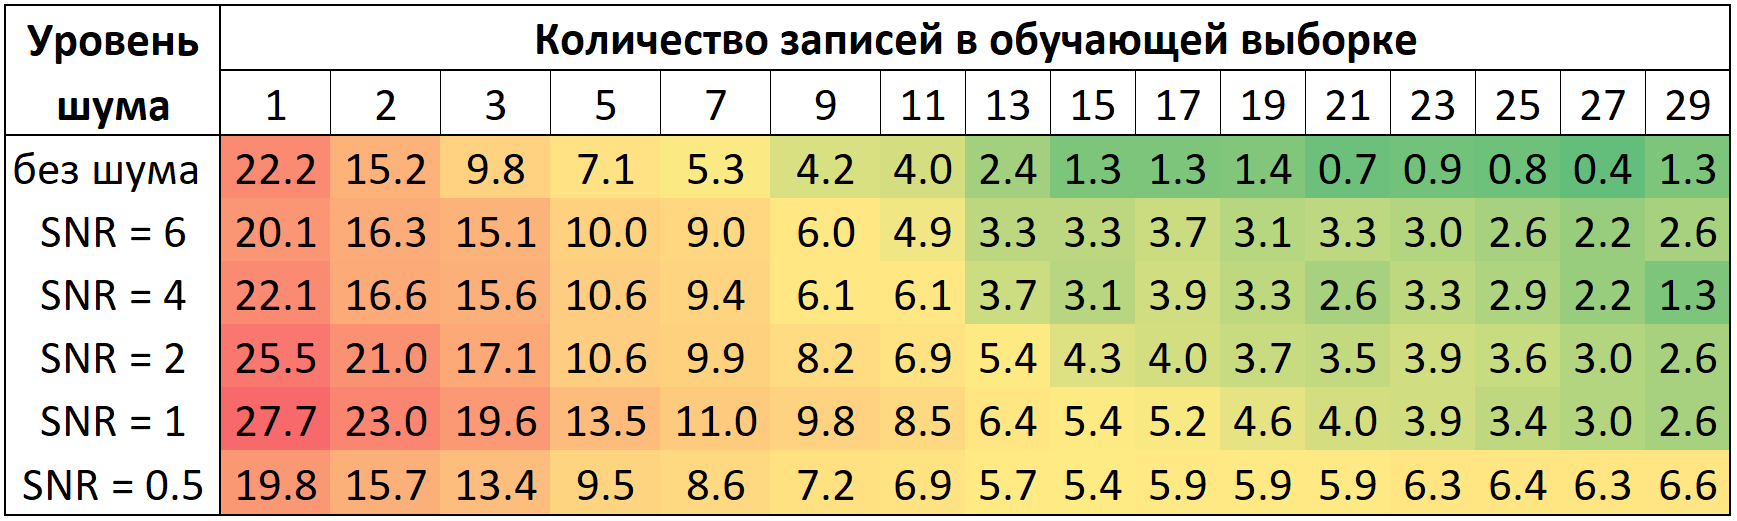
\includegraphics[width=1.0\textwidth]{cnn_phrases_self_noise.png}
	\caption{Усреднённые результаты распознавания фраз свёрточной нейронной сетью в условиях различных уровней шума при обучении на том же дикторе, в таблице указан процент неправильных распознаваний}
	\label{fig:cnn_phrases_self_noise}
\end{figure}

В данных результатах, аналогично результатам распознавания слов, видно плавное повышение процента ошибок при увеличении уровня шума, при этом по величине повышение оказывается не очень большим.
Например, при использовании 13 записей в обучающей выборке при отсутствии шума получается 2.4~\% ошибок, а при отношении сигнал/шум равном 1 получается 6.4~\% ошибок.
Аналогичные значения при обучении на 9 записях равны 4.2 и 9.8~\% соответственно.
Данные результаты показывают, к каким величинам ошибок нужно стремиться при распознавании фраз с шумом других дикторов для исключения эффекта дикторозависимости.

Далее отношение сигнал/шум принималось равным 4.
Также были эксперименты с наложением нескольких различных вариантов шумов на одни и те же записи.
Для начала было проведено обычное распознавание фраз одним диктором с наложением одного варианта шума.
В таблице \ref{tab:cnn_phrases_1dictor_1noise} представлено 2 варианта эксперимента.

\begin{table}[h]
	\centering
	\caption{Результаты распознавания фраз для случая записей с шумом при распознавании на обучающем наборе из одного диктора с 1 вариантом шума, в таблице указан процент неправильных распознаваний}
	\label{tab:cnn_phrases_1dictor_1noise}
	\begin{tabular}{| l | c | c | c | c | c | c | c |}
		\hline
		Набор & \multicolumn{7}{c|}{Диктор для распознавания} \\
		\hhline{~-------}
		обучения \phantom{0000} & \phantom{0} АП \phantom{0} & \phantom{0} ВП \phantom{0} & \phantom{0} ЛД \phantom{0} & \phantom{0} МЛ \phantom{0} & \phantom{0} НМ \phantom{0} & \phantom{0} ОР \phantom{0} & \phantom{0} ОП \phantom{0} \\
		\hline
		\multicolumn{8}{|c|}{обучение с шумом, распознавание без шума} \\
		\hline
		АП		 &  0.0 & 38.5 & 45.5 & 15.2 & 34.8 & 50.0 & 11.8 \\
		ВП		 & 40.3 &  0.6 & 16.7 & 31.2 & 15.8 & 21.2 & 17.3 \\
		ЛД		 & 47.0 & 19.4 &  0.0 & 24.5 & 15.8 & 22.4 & 24.5 \\
		МЛ		 & 20.0 & 17.0 & 22.1 &  0.6 & 19.7 & 15.8 &  1.2 \\
		НМ		 & 41.2 &  7.6 & 15.8 & 25.2 &  0.0 & 12.4 & 10.3 \\
		ОР		 & 48.2 & 14.2 & 23.0 & 36.4 & 17.3 &  0.0 & 18.8 \\
		ОП		 & 22.1 & 16.4 & 33.9 & 17.0 & 18.2 & 26.7 &  0.6 \\
		\hline
		\multicolumn{8}{|c|}{обучение с шумом, распознавание с шумом} \\
		\hline
		АП		 &  0.0 & 36.1 & 46.1 & 21.5 & 37.6 & 49.4 & 17.6 \\
		ВП		 & 33.6 &  0.0 & 12.1 & 24.2 & 10.9 & 20.9 & 11.5 \\
		ЛД		 & 44.8 & 14.8 &  0.0 & 26.1 & 14.8 & 33.9 & 19.1 \\
		МЛ		 & 12.7 & 18.5 & 17.9 &  0.0 & 12.1 & 20.3 &  3.6 \\
		НМ		 & 37.3 &  8.5 & 10.6 & 23.6 &  0.0 & 29.1 & 10.6 \\
		ОР		 & 47.3 & 13.3 & 20.6 & 33.9 & 15.2 &  0.0 & 17.0 \\
		ОП		 & 21.5 & 18.5 & 23.3 & 11.8 & 14.2 & 22.4 &  0.0 \\
		\hline
	\end{tabular}
\end{table}

В первом случае обучение проводилось на фразах с шумом, а распознавались фразы без шума.
Средняя ошибка при распознавании записей диктора, на которых проводилось обучение, равна 0.3~\%, а средняя ошибка для записей других дикторов --- 23.6~\%.
Во втором случае и обучение, и распознавание проводилось на записях с шумом.
На записях, на которых проводилось обучение, ошибок не было, а средняя ошибка для записей других дикторов равна 22.4~\%.
Из этих результатов видно, что для обоих вариантов распознавания ошибка получается выше, чем при использовании записей без шума.
Более того, аналогично распознаванию слов распознавание записей с шумом показало меньшую ошибку, чем распознавание записей без шума.
В дальнейшем будет использоваться только распознавание записей с шумом.

Далее был проведён аналогичный эксперимент, но с тем отличием, что для обучения использовались записи с 5 и 10 наложенными различными вариантами шума.
Для первого эксперимента с 5 вариантами шума средняя ошибка при распознавании записей диктора, на которых проводилось обучение, равна 0.0~\%, а средняя ошибка для записей других дикторов --- 21.1~\%.
Для второго эксперимента с 10 вариантами шума на записях, на которых проводилось обучение, ошибок не было, а средняя ошибка для записей других дикторов равна 20.8~\%.
Как видно из приведённых результатов, использование нескольких вариантов шумов заметно улучшает качество распознавания по сравнению с 1 вариантом шума.
Результаты данных экспериментов приведены в таблице \ref{tab:cnn_phrases_1dictor_noises}.

\begin{table}[h]
	\centering
	\caption{Результаты распознавания фраз для случая записей с шумом при распознавании на обучающем наборе из одного диктора с 5 и 10 вариантами шума, в таблице указан процент неправильных распознаваний}
	\label{tab:cnn_phrases_1dictor_noises}
	\begin{tabular}{| l | c | c | c | c | c | c | c |}
		\hline
		Набор & \multicolumn{7}{c|}{Диктор для распознавания} \\
		\hhline{~-------}
		обучения \phantom{0000} & \phantom{0} АП \phantom{0} & \phantom{0} ВП \phantom{0} & \phantom{0} ЛД \phantom{0} & \phantom{0} МЛ \phantom{0} & \phantom{0} НМ \phantom{0} & \phantom{0} ОР \phantom{0} & \phantom{0} ОП \phantom{0} \\
		\hline
		\multicolumn{8}{|c|}{5 вариантов шума} \\
		\hline
		АП 		 &  0.0 & 35.5 & 43.9 & 17.9 & 40.0 & 42.7 & 15.8 \\
		ВП 		 & 33.0 &  0.0 &  9.4 & 23.3 & 10.9 & 22.7 & 13.0 \\
		ЛД		 & 42.1 & 10.3 &  0.0 & 23.3 & 12.1 & 28.8 & 18.8 \\
		МЛ		 & 11.5 & 14.5 & 13.6 &  0.0 & 13.3 & 17.6 &  3.0 \\
		НМ		 & 42.7 & 10.9 & 13.0 & 23.3 &  0.0 & 27.3 & 10.9 \\
		ОР		 & 47.0 & 11.5 & 19.4 & 33.0 & 11.2 &  0.0 & 13.0 \\
		ОП		 & 23.0 & 14.2 & 21.2 & 12.4 & 12.1 & 23.6 &  0.0 \\
		\hline
		\multicolumn{8}{|c|}{10 вариантов шума} \\
		\hline
		АП		 &  0.0 & 37.0 & 45.8 & 18.5 & 38.5 & 44.5 & 15.2 \\
		ВП		 & 35.2 &  0.0 & 16.7 & 23.9 & 10.9 & 19.7 & 10.9 \\
		ЛД		 & 40.0 & 10.6 &  0.0 & 20.9 & 10.9 & 28.8 & 15.5 \\
		МЛ		 & 11.8 & 13.0 & 12.7 &  0.0 &  9.7 & 16.7 &  2.4 \\
		НМ		 & 44.8 & 10.9 & 10.9 & 23.3 &  0.0 & 27.9 & 10.9 \\
		ОР		 & 48.2 & 15.8 & 22.4 & 29.4 & 14.2 &  0.0 & 12.4 \\
		ОП		 & 23.6 & 13.6 & 19.7 &  9.7 & 10.6 & 17.0 &  0.0 \\
		\hline
	\end{tabular}
\end{table}

После этого было проведено обучение нейронной сети на 3 дикторах в условиях шума и последующее распознавания записей.
Первый эксперимент предполагает использование одного варианта шума при обучении, а второй эксперимент --- 5 вариантов шума.
В обоих случаях средняя величина ошибки при распознавании записей диктора, на которых проводилось обучение, равна 0.0~\%.
Для случая распознавания записей других дикторов ошибка равна 11.5~\% для первого эксперимента и 10.4~\% для второго.
Подробные результаты экспериментов приведены в таблице \ref{tab:cnn_phrases_3dictors_noises}.

\begin{table}[h]
	\centering
	\caption{Результаты распознавания фраз для случая записей с шумом при распознавании на обучающем наборе из трёх дикторов с 1 и 5 вариантами шума, в таблице указан процент неправильных распознаваний}
	\label{tab:cnn_phrases_3dictors_noises}
	\begin{tabular}{| l | c | c | c | c | c | c | c |}
		\hline
		Набор & \multicolumn{7}{c|}{Диктор для распознавания} \\
		\hhline{~-------}
		обучения \phantom{0000} & \phantom{0} АП \phantom{0} & \phantom{0} ВП \phantom{0} & \phantom{0} ЛД \phantom{0} & \phantom{0} МЛ \phantom{0} & \phantom{0} НМ \phantom{0} & \phantom{0} ОР \phantom{0} & \phantom{0} ОП \phantom{0} \\
		\hline
		\multicolumn{8}{|c|}{1 вариант шума} \\
		\hline
		АП,ВП,ЛД &  0.0 & 0.0 &  0.0 &  8.2 &  6.4 & 20.3 & 6.4 \\
		ВП,ЛД,МЛ & 14.5 & 0.0 &  0.0 &  0.0 &  6.1 & 17.3 & 3.9 \\
		ЛД,МЛ,НМ & 16.4 & 7.0 &  0.0 &  0.0 &  0.0 & 17.9 & 1.8 \\
		МЛ,НМ,ОР & 17.6 & 7.0 &  7.9 &  0.0 &  0.0 &  0.0 & 1.5 \\
		НМ,ОР,ОП & 28.2 & 9.7 & 11.2 & 15.8 &  0.0 &  0.0 & 0.0 \\
		ОР,ОП,АП &  0.0 & 9.1 & 20.6 &  7.0 & 12.4 &  0.0 & 0.0 \\
		ОП,АП,ВП &  0.0 & 0.0 & 12.7 &  8.2 &  9.1 & 18.5 & 0.0 \\
		\hline
		\multicolumn{8}{|c|}{5 вариантов шума} \\
		\hline
		АП,ВП,ЛД &  0.0 & 0.0 &  0.0 &  8.2 &  8.2 & 17.3 & 4.5 \\
		ВП,ЛД,МЛ & 13.6 & 0.0 &  0.0 &  0.0 &  7.6 & 14.2 & 0.9 \\
		ЛД,МЛ,НМ & 15.5 & 5.8 &  0.0 &  0.0 &  0.0 & 18.2 & 2.4 \\
		МЛ,НМ,ОР & 17.9 & 8.2 &  5.8 &  0.0 &  0.0 &  0.0 & 1.2 \\
		НМ,ОР,ОП & 27.6 & 6.4 &  9.1 & 13.6 &  0.0 &  0.0 & 0.0 \\
		ОР,ОП,АП &  0.0 & 7.3 & 15.8 &  7.9 & 11.2 &  0.0 & 0.0 \\
		ОП,АП,ВП &  0.0 & 0.0 & 12.1 &  6.7 & 10.6 & 13.3 & 0.0 \\
		\hline
	\end{tabular}
\end{table}

Здесь также видно улучшение при увеличении вариантов шума в обучающей выборке.

Результаты эксперимента на фразах с наложенным шумом при обучении на 7 дикторах приведены в таблице \ref{tab:cnn_phrases_7dictors_noises}.

\begin{table}[h]
	\centering
	\caption{Результаты распознавания фраз для случая записей с шумом при распознавании на обучающем наборе из семи дикторов с 1 и 2 вариантами шума, в таблице указан процент неправильных распознаваний}
	\label{tab:cnn_phrases_7dictors_noises}
	\begin{tabular}{| l | c | c | c | c | c | c | c |}
		\hline
		Набор & \multicolumn{7}{c|}{Диктор для распознавания} \\
		\hhline{~-------}
		обучения & \phantom{0}АП\phantom{0} & \phantom{0}ВП\phantom{0} & \phantom{0}ЛД\phantom{0} & \phantom{0}МЛ\phantom{0} & \phantom{0}НМ\phantom{0} & \phantom{0}ОР\phantom{0} & \phantom{0}ОП\phantom{0} \\
		\hline
		\multicolumn{8}{|c|}{1 вариант шума} \\
		\hline
		АП,ВП,ЛД,МЛ,НМ,ОР &  0.0 & 0.0 & 0.0 & 0.0 & 0.0 &  0.0 & 2.4 \\
		ВП,ЛД,МЛ,НМ,ОР,ОП & 16.7 & 0.0 & 0.0 & 0.0 & 0.0 &  0.0 & 0.0 \\
		ЛД,МЛ,НМ,ОР,ОП,АП &  0.0 & 5.5 & 0.0 & 0.0 & 0.0 &  0.0 & 0.0 \\
		МЛ,НМ,ОР,ОП,АП,ВП &  0.0 & 0.0 & 5.2 & 0.0 & 0.0 &  0.0 & 0.0 \\
		НМ,ОР,ОП,АП,ВП,ЛД &  0.0 & 0.0 & 0.0 & 7.9 & 0.0 &  0.0 & 0.0 \\
		ОР,ОП,АП,ВП,ЛД,МЛ &  0.0 & 0.0 & 0.0 & 0.0 & 5.5 &  0.0 & 0.0 \\
		ОП,АП,ВП,ЛД,МЛ,НМ &  0.0 & 0.0 & 0.0 & 0.0 & 0.0 & 15.8 & 0.0 \\
		\hline
		\multicolumn{8}{|c|}{2 варианта шума} \\
		\hline
		АП,ВП,ЛД,МЛ,НМ,ОР &  0.0 & 0.0 & 0.0 & 0.0 & 0.0 &  0.0 & 1.2 \\
		ВП,ЛД,МЛ,НМ,ОР,ОП & 13.9 & 0.0 & 0.0 & 0.0 & 0.0 &  0.0 & 0.0 \\
		ЛД,МЛ,НМ,ОР,ОП,АП &  0.0 & 6.1 & 0.0 & 0.0 & 0.0 &  0.0 & 0.0 \\
		МЛ,НМ,ОР,ОП,АП,ВП &  0.0 & 0.0 & 6.1 & 0.0 & 0.0 &  0.0 & 0.0 \\
		НМ,ОР,ОП,АП,ВП,ЛД &  0.0 & 0.0 & 0.0 & 7.0 & 0.0 &  0.0 & 0.0 \\
		ОР,ОП,АП,ВП,ЛД,МЛ &  0.0 & 0.0 & 0.0 & 0.0 & 3.6 &  0.0 & 0.0 \\
		ОП,АП,ВП,ЛД,МЛ,НМ &  0.0 & 0.0 & 0.0 & 0.0 & 0.0 & 10.9 & 0.0 \\
		\hline
	\end{tabular}
\end{table}

В данном эксперименте при обучении использовались один и два варианта шума.
Большее количество шумов не удалось использовать из-за ограничений вычислительной мощности компьютера.
Для обоих вариантов обучения, при распознавании фраз из обучающей выборки ошибок нет.
При использовании одного варианта шума, для распознавания фраз из тестовой выборки получается в среднем 8.4~\% ошибок, а при использовании двух вариантов шума --- 7.0~\% ошибок.

В таблице \ref{tab:cnn_phrases_with_noise_summary} приведены итоговые результаты распознавания фраз в условиях шума при обучении на различном числе дикторов и различном количестве наложенных шумов.

\begin{table}[h]
	\centering
	\caption{Суммарные результаты распознавания по <<своему>> и <<чужому>> диктору при обучении на различном числе дикторов для случаев записей фраз без шума и с шумом, в таблице указан процент неправильных распознаваний}
	\label{tab:cnn_phrases_with_noise_summary}
	\begin{tabular}{| l | c | c | c | c |}
		\hline
		Число				& \phantom{0}Наличие\phantom{0} & \phantom{0} Число \phantom{0} 	& \multicolumn{2}{c|}{Процент ошибок}	\\
		\hhline{~~~--}
		дикторов			& шума  			& шумов 	& обучающая выборка & тестовая выборка	\\
		\hline
		\multirow{4}{*}{1 диктор}	& без шума					& 1				& 0.3 		& 23.6 		\\
		\hhline{~----}
									& \multirow{3}{*}{с шумом}	& 1				& 0.0 		& 22.4  	\\
		\hhline{~~---}
									&							& 5				& 0.0 		& 21.1  	\\
		\hhline{~~---}
									&    						& 10			& 0.0 		& 20.8  	\\
		\hline
		\multirow{2}{*}{3 диктора}	& \multirow{2}{*}{с шумом}	& 1				& 0.0 		& 11.5  	\\
		\hhline{~~---}
									&    						& 5				& 0.0 		& 10.4  	\\
		\hline
		\multirow{2}{*}{6 дикторов}	& \multirow{2}{*}{с шумом}	& 1				& 0.0 		& 8.4  		\\
		\hhline{~~---}
									&    						& 2				& 0.0 		& 7.0  		\\
		\hline
	\end{tabular}
\end{table}

Здесь получается вывод, полностью аналогичный выводу, полученному в экспериментах распознавания слов в условиях шума: процент ошибок стабильно снижается при увеличении количества дикторов в обучающей базе и увеличение числа накладываемых шумов приводит к уменьшению числа ошибок, но уменьшение меньше, чем при увеличении количества дикторов.

В целом, результаты распознавания фраз очень похожи на результаты распознавания слов, как в условиях без шума, так и в условиях с шумом.
Единственное отличие --- это заметно большее количество ошибок.
Это можно объяснить тем, что при произношении фраз большую роль играет длительность паузы между словами, в то время как при распознавании слов такой проблемы не возникает.
Но, в любом случае, свёрточные нейронные сети показали лучшие результаты для задачи распознавания фраз.

\clearpage

%\newpage
%============================================================================================================================

\section{Улучшение качества распознавания отдельных фраз при дополнительном обучении} \label{sect4_6}

В конце был проведён эксперимент по расширению обучающей выборки и исследованию изменения качества распознавания.
Эксперимент заключался в следующем.
Предположим, что у нас есть обучающая выборка из записей одного или нескольких дикторов.
Нейронная сеть обучается на данной выборке.
После этого с помощью нейронной сети распознаются записи другого диктора, не входящего в обучающую выборку.
Таким образом, реализуется вариант распознавания по <<чужому>> диктору.

После этого было проверено изменение качества распознавания команд при обучении по записям чужого диктора с добавлением небольшого числа записей своего диктора, то есть того, чьи записи будут потом распознаваться.
При этом, несмотря на то, что записи из обучающей выборки и записи для распознавания будут принадлежать одному диктору, это будут разные реализации команд, то есть добавленные к обучающей выборке записи исключаются из тестовой выборки.
В обучающую выборку добавлялось 1, 2, 3, 5, 10 и 15 записей своего диктора.
Таким образом, можно учесть некоторые индивидуальные особенности распознаваемого диктора при добавлении лишь небольшого числа записей, что достаточно несложно реализуется на практике.

В таблице \ref{tab:cnn_phrases_addition} приведены результаты распознавания в эксперименте для различных наборов параметров.
В строках указано количество использованных в обучающей выборке <<чужих>> дикторов.
По столбцам отложено количество записей каждого слова <<своего>> диктора, добавленных в обучающую выборку.

\begin{table}[h]
	\centering
	\caption{Процент ошибок распознавания фраз при добавлении различного количества записей к обучающей выборке, состоящей из записей одного или нескольких дикторов}
	\label{tab:cnn_phrases_addition}
	\begin{tabular}{| l | c | c | c | c | c | c | c |}
		\hline
		Число & \multicolumn{7}{c|}{Число добавленных записей} \\
		\hhline{~-------}
		дикторов \phantom{000} & \phantom{00} 0 \phantom{00} & \phantom{00} 1 \phantom{00} & \phantom{00} 2 \phantom{00} & \phantom{00} 3 \phantom{00} & \phantom{00} 5 \phantom{00} & \phantom{00} 10 \phantom{00} & \phantom{00} 15 \phantom{00} \\
		\hline
		1 		 & 18.0 & 8.8 & 7.2 & 6.4 & 5.2 & 3.7 & 1.9 \\
		2 		 & 11.4 & 7.1 & 6.1 & 5.2 & 4.8 & 3.6 & 1.6 \\
		3 		 &  6.9 & 5.2 & 4.8 & 4.3 & 3.8 & 3.1 & 1.2 \\
		4 		 &  5.4 & 4.6 & 3.7 & 3.7 & 3.2 & 2.7 & 1.1 \\
		5 		 &  4.8 & 4.3 & 4.1 & 3.9 & 3.5 & 2.7 & 1.2 \\
		6 		 &  4.2 & 3.9 & 3.8 & 3.7 & 3.2 & 2.9 & 1.2 \\
		\hline
	\end{tabular}
\end{table}

Как видно из результатов, при добавлении всего по одной реализации каждой из речевых команд <<своего>> диктора в обучающую выборку ошибка распознавания уменьшается более чем в 2 раза с 18.6 до 8.8~\%.
Дальнейшее добавление записей снижает ошибку, но величина снижения уже не такая большая.
Также, эффект от добавленных записей тем больше, чем меньше дикторов использовано в обучающей выборке.
Это объясняется тем, что при маленьком числе дикторов в обучающей выборке высока степень переобучения для конкретного диктора, поэтому добавление записей другого диктора хорошо снижает степень такого переобучения.
Для обучающих выборок из нескольких дикторов переобучение меньше, поэтому меньше и улучшение.
При добавлении нескольких реализаций слов процент ошибок продолжает снижаться, но меньшими темпами.
Практический результат данного эксперимента состоит в том, что добавление небольшого числа записей к большой обучающей выборке заметно влияет на точность распознавания.

%\newpage
%============================================================================================================================

\section{Выводы по разработке алгоритмов на основе свёрточных нейронных сетей} \label{sect4_7}

В данном разделе описаны предложенные алгоритмы распознавания речевых команд на основе свёрточных нейронных сетей.
В начале описана используемая среда разработки и применённая параметризация обучающей выборки и распознаваемых речевых записей.
После этого проведён анализ работоспособности традиционных нейронных сетей типа одно- и двухслойных персептронов.
Средняя полученная доля неправильно распознанных слов на тестовой выборке получилась высокой и составила 20--25~\%.

Далее была предложена архитектура свёрточной нейронной сети и проведён подбор параметров данной сети.
Затем для нескольких поставленных задач производилось обучение и проверка результатов работы алгоритма.
Первой задачей было распознавание записей <<своего>> диктора.
Результаты показали, что можно добиться ошибки распознавания в 2~\% при использовании 7 записей каждого слова в обучающей выборке и ошибки в 0.5~\% для 20 записей.

Вторая задача заключалась в обучении на записях одного или нескольких дикторов и распознавании записей <<чужого>> диктора.
Здесь удалось получить долю ошибок равную 5.9~\% для обучающей выборки из одного диктора, 1.7~\% для выборки из 3 дикторов и 0.6~\% для 7 дикторов.
Последний результат является очень хорошим, так как результат распознавания <<чужого>> диктора вплотную приближается к результату распознавания по <<своему>> диктору.

Третья задача подразумевала проверку работоспособности свёрточных нейронных сетей при обучении и распознавании записей с шумом.
Для этого уникальные части шума кабины пилота добавлялись ко всем записям.
При распознавании записей <<своего>> диктора количество ошибок увеличилось примерно в 2 раза при использовании отношения сигнал/шум равного 1.
Также было показано стабильное, но не очень большое по величине повышение числа ошибок при увеличении уровня шума.
При распознавании записей <<чужого>> диктора были получены ошибки равные 9.7~\% при обучении на записях одного диктора с одним добавленным шумом, а если добавлялось 7 различных вариантов шума в обучающую выборку, то ошибка снижалась до 8.2~\%.
Для 3 дикторов процент ошибок был 2.8~\% для одно варианта шума и 2.5~\% для 3 вариантов.
Для 7 дикторов эти значения были соответственно 1.2 и 1.1~\%, что является крайне низким значением при распознавании в условиях шума.

После этого были проведены аналогичные эксперименты для речевых команд в форме фраз.
Для распознавания по <<своему>> диктору было получено около 1~\% ошибок при размере обучающей выборки в 20 записей каждого слова.
Распознавание по <<чужому>> диктору показало 18~\% ошибок при обучении по записям одного диктора, 6.9~\% ошибок при 3 дикторах и 4.2~\% для 6 дикторов.
При распознавании записей <<своего>> диктора в условиях шума получены результаты аналогичные случаю распознавания слов.
При распознавании записей <<чужих>> дикторов с шумом для 1 диктора получилось от 20.8 до 23.6~\% ошибок и от 7.0 до 8.4~\% ошибок для обучающей выборки из записей 6 дикторов.

В конце был рассмотрен способ улучшения качества распознавания за счёт добавлению к обучающей выборке небольшого количества записей <<своего>> диктора.
Получилось, что при добавлении всего 1 реализации каждого слова в обучающую выборку, состоящую из записей одного диктора, доля ошибок снижалась с 18 до 8.8~\%, а при добавлении 3 записей до 6.4~\%.
Для обучающей выборки из 3 дикторов при добавлении одной записи было зафиксировано снижение числа неправильных распознаваний с 6.9 до 5.2~\%, а при добавлении 3 записей до 4.3~\%.
По результатам видно, что добавление всего лишь 1 записи каждого слова <<своего>> диктора приводит к сильному снижению процента ошибок распознавания, особенно при обучении на выборках с записями малого количества дикторов.

%\newpage
%============================================================================================================================

\clearpage           % Глава 4
\chapter*{Заключение}                       % Заголовок
\addcontentsline{toc}{chapter}{Заключение}  % Добавляем его в оглавление

%% Согласно ГОСТ Р 7.0.11-2011:
%% 5.3.3 В заключении диссертации излагают итоги выполненного исследования, рекомендации, перспективы дальнейшей разработки темы.
%% 9.2.3 В заключении автореферата диссертации излагают итоги данного исследования, рекомендации и перспективы дальнейшей разработки темы.
%% Поэтому имеет смысл сделать эту часть общей и загрузить из одного файла в автореферат и в диссертацию:

Основные результаты работы заключаются в следующем.
%% Согласно ГОСТ Р 7.0.11-2011:
%% 5.3.3 В заключении диссертации излагают итоги выполненного исследования, рекомендации, перспективы дальнейшей разработки темы.
%% 9.2.3 В заключении автореферата диссертации излагают итоги данного исследования, рекомендации и перспективы дальнейшей разработки темы.

\begin{enumerate}[label={\arabic*)}]
	\item Разработан автоматический алгоритм разбиения слов на однородные части, в основе которого нахождение положения границ частей производится с помощью многопараметрической оптимизации.
	Сформулированы критерии, реализующие принцип максимизации меры сходства фонетического материала внутри части и меры различия между соседними частями. 
	Для численного решения задачи с высоким быстродействием предложены алгоритмы, основанные на методе динамического программирования.
	Эксперименты, проведённые на примерах нескольких слов русского языка, подтвердили работоспособность предложенного подхода и правомерность принятых допущений.
	\item Разработан алгоритм улучшения качества эталона, основанный на выделении и оптимизации главных компонент.
	Эталон, полученный с помощью оптимизации коэффициентов при главных компонентах, показал значительно меньшее число ошибок при распознавании большинства записей.
	Общее количество ошибок для записей слов с шумом в наушниках до оптимизации равнялось 5~\%, а после оптимизации уменьшилось до 1.25~\%.
	Также был сделан вывод о том, что для получения приемлемых результатов достаточно использовать только одну реализацию слова и проводить всего 10 итераций при получении оптимального эталона, что заметно сокращает время работы программы.
	\item Изучены способы и разработаны алгоритмы сжатия информации о параметрическом портрете с помощью применения полиномов Чебышёва.
	Эксперименты показали, что сжатие может происходить как отдельно по частотам и по времени, так и по обоим измерениям одновременно.
	В последнем случае можно сократить место для хранения параметрического портрета в 5--10 раз практически без ухудшения качества распознавания.	
	\item Разработаны алгоритмы на основе формулы Байеса и метода комитетов, позволяющие заметно уменьшить количество ошибок распознавания при использовании нескольких эталонов.
	Первый алгоритм использует оценки априорных вероятностей, определяемые по обучающей выборке, и рассчитывает апостериорные вероятности формулы Байеса, а второй является модификацией известного метода комитетов.
	Выявленная в ходе тестирования возможность локализации распознаваемого слова с точностью до малой группы позволяет повышать быстродействие систем распознавания на основе иерархических процедур, в которых последовательно применяются алгоритмы распознавания разных видов.
	Работоспособность обоих разработанных алгоритмов подтверждается результатами тестирования.
	При использовании 7 эталонов, полученных по записям различных дикторов, достигается заметное снижение процента ошибок в 1.5--2 раза --- средняя ошибка для алгоритма на основе формулы Байеса снизилась с 8.42 до 5.62~\%, а для алгоритма на основе метода комитетов до 5.3 и до 3.13~\% при использовании подстройки по времени.
	\item Изучены и модифицированы алгоритмы распознавания речевых команд на основе искусственных нейронных сетей глубокого обучения.
	Наилучшие результаты показала архитектура нейронных сетей CNN с двумя слоями свёртки и тремя полностью связанными слоями.
	При обучении на словаре из 20 слов без шума на 7 дикторах средняя величина ошибки при распознавании <<чужих>> дикторов равна 0.6~\%.
	При обучении в той же конфигурации, но на записях с добавленным шумом, величина ошибки достигает для <<чужого>> диктора 1.1~\%.
	Эксперименты по распознаванию фраз при использовании обучающей выборки из записей 6 дикторов показали 4.2~\% ошибок для случая без шума и 7.0~\% для записей с шумом.
	Получены положительные результаты в дикторозависимом варианте распознавания без шума и в условиях шума при использовании небольшого числа записей каждой команды в обучающей выборке.
	Также получено значительное улучшение качества распознавания при добавлении всего нескольких реализаций каждой из речевых команд <<своего>> диктора в обучающую выборку, состоящую из записей <<чужих>> дикторов.
	При использовании нейронных сетей CNN количество ошибок является заметно более низким, чем для других алгоритмов, единственный замеченный недостаток --- это длительное время обучения нейронной сети.
\end{enumerate}


В заключение автор выражает благодарность и большую признательность научному руководителю Корсуну Олегу Николаевичу за поддержку, помощь, обсуждение результатов и научное руководство.

      % Заключение
%\include{Dissertation/acronyms}	   % Список сокращений и условных обозначений
%\include{Dissertation/dictionary}	   % Словарь терминов
\include{Dissertation/references}      % Список литературы
%\include{Dissertation/lists}          % Списки таблиц и изображений (иллюстративный материал)

%%% Настройки для приложений
%\appendix
% Оформление заголовков приложений ближе к ГОСТ:
\setlength{\midchapskip}{20pt}
\renewcommand*{\afterchapternum}{\par\nobreak\vskip \midchapskip}
\renewcommand\thechapter{\Asbuk{chapter}} % Чтобы приложения русскими буквами нумеровались

%\include{Dissertation/appendix}        % Приложения

\end{document}
